\documentclass[12pt,twoside,letterpaper,titlepage]{report}

\usepackage{amssymb,amsmath}
\usepackage{mathspec}
\defaultfontfeatures{Ligatures=TeX,Scale=MatchLowercase}
\usepackage[margin=1.0in]{geometry}
% fixltx2e has been merged into LaTeX2e proper
% see: https://latex-project.org/ltnews/ltnews22.pdf
% \usepackage{fixltx2e}
\usepackage{graphicx,grffile}
\makeatletter
\def\maxwidth{\ifdim\Gin@nat@width>\linewidth\linewidth\else\Gin@nat@width\fi}
\def\maxheight{\ifdim\Gin@nat@height>\textheight\textheight\else\Gin@nat@height\fi}
\makeatother
% Scale images if necessary, so that they will not overflow the page
% margins by default, and it is still possible to overwrite the defaults
% using explicit options in \includegraphics[width, height, ...]{}
\setkeys{Gin}{width=\maxwidth,height=\maxheight,keepaspectratio}
\usepackage[table,svgnames]{xcolor}
\usepackage{framed}
\usepackage{longtable,booktabs}
\usepackage{listings}
\PassOptionsToPackage{hyphens}{url}\usepackage[breaklinks=true]{hyperref}

% Background Color for Note/Admonition Boxes
\definecolor{shadecolor}{rgb}{0.9,0.9,0.9}

% Band the Color of Rows in Tables
% unfortunately, doesn't seem to work across the board. Turning off for now
%\rowcolors{1}{white}{lightgray!25!white}

\newenvironment{callout}{\begin{shaded*}\small}{\end{shaded*}}
\newcommand{\warning}[1]{\small{\textbf{\textcolor[rgb]{0.8,0.2,0.2}{#1}}}}

% Font Settings
%\setmainfont[]{Calibri}
%\setmonofont[Mapping=tex-ansi]{Inconsolata}
%\usepackage{newtxtext,newtxmath}

% The depth of numbering for sections
\setcounter{secnumdepth}{4}

% Listing Settings
\lstset{
  backgroundcolor=\color{BlanchedAlmond!20!white},
  basicstyle=\ttfamily\scriptsize,
  breakatwhitespace=false,
  breaklines=true,
  frame=bottomline,
  keepspaces=true,
}

% Provide better table spacing
% From https://www.inf.ethz.ch/personal/markusp/teaching/guides/guide-tables.pdf
\renewcommand{\arraystretch}{1.2} 

\graphicspath{{media/}}

\pagestyle{headings}

% Define custom commands from Pandoc
\setlength{\emergencystretch}{3em}  % prevent overfull lines
\providecommand{\tightlist}{%
  \setlength{\itemsep}{0pt}\setlength{\parskip}{0pt}}

% Redefine (sub)paragraphs to behave more like sections
\ifx\paragraph\undefined\else
\let\oldparagraph\paragraph
\renewcommand{\paragraph}[1]{\oldparagraph{#1}\mbox{}}
\fi
\ifx\subparagraph\undefined\else
\let\oldsubparagraph\subparagraph
\renewcommand{\subparagraph}[1]{\oldsubparagraph{#1}\mbox{}}
\fi

% this is a great package for printing units in a standard way, we should move this way
\usepackage{siunitx}

% some additional macros
\newcommand{\PB}[1]{\left(#1\right)}
\newcommand{\RB}[1]{\left[#1\right]}
\newcommand{\CB}[1]{\left\{#1\right\}}

\author{U.S. Department of Energy}
\date{September 30, 2016}


\title{Tips and Tricks for Using EnergyPlus}

\hypersetup{unicode=true,
            pdftitle={Tips and Tricks for Using EnergyPlus},
            pdfauthor={U.S. Department of Energy},
            colorlinks=true,
            linkcolor=Maroon,
            citecolor=Blue,
            urlcolor=Blue,
            breaklinks=true}
\urlstyle{same}  % don't use monospace font for urls

\begin{document}


% Reference for making your own Title Page: 
% http://tex.stackexchange.com/questions/10130/use-the-values-of-title-author-and-date-on-a-custom-title-page
\makeatletter
\begin{titlepage}
  \begin{center}
    {\scshape\LARGE EnergyPlus\texttrademark{} Version 8.6 Documentation \par}
    \vspace{1.5cm}
    {\bfseries\huge \@title \par}
    \vspace{1.5cm}
    {\Large\itshape \@author \par}
    \vspace{2.5cm}
    
\includegraphics[width=0.2\textwidth]{media/ep.png}\par\vspace{1cm}
    \vfill

    % Bottom of the page
    {\large \@date \par}
    \vspace{1.5cm}
  \end{center}
  {\small
COPYRIGHT (c) 1996-2016 THE BOARD OF TRUSTEES OF THE UNIVERSITY OF ILLINOIS AND THE REGENTS OF THE UNIVERSITY OF CALIFORNIA THROUGH THE ERNEST ORLANDO LAWRENCE BERKELEY NATIONAL LABORATORY. ALL RIGHTS RESERVED. NO PART OF THIS MATERIAL MAY BE REPRODUCED OR TRANSMITTED IN ANY FORM OR BY ANY MEANS WITHOUT THE PRIOR WRITTEN PERMISSION OF THE UNIVERSITY OF ILLINOIS OR THE ERNEST ORLANDO LAWRENCE BERKELEY NATIONAL LABORATORY. ENERGYPLUS IS A TRADEMARK OF THE US DEPARTMENT OF ENERGY.
  }
\end{titlepage}
\makeatother

{
\setcounter{tocdepth}{2}
\tableofcontents
}

\hypertarget{generated-toc}{}



\chapter{Introduction \& Support}\label{introduction-support}

This is a quick guide for using and troubleshooting EnergyPlus simulation software. The information here is taken from the knowledge base and from EnergyPlus users looking for answers.

\textbf{Note that these articles are taken from actual user questions and may not be applicable to your model.}

For more detailed information about using EnergyPlus, refer to the user guides and manuals that are installed in the Documentation folder and are also available from \href{http://www.energyplus.gov}{www.energyplus.gov}.

This is a short guide

\ldots{} meant to save time and energy!


\section{Organization}\label{organization}

This document begins with some general information to introduce users to the syntax used in EnergyPlus as well as this guide. Then some basic conversion methods needed to take a real system and format it to simplify the input process are provided. The bulk of this Application Guide is devoted to modeling example systems. The example systems are intended to demonstrate the input process for various types of plant systems, such as systems that use thermal energy storage tanks and those that have a primary/secondary pumping configurations.

The example systems are defined by breaking the system into its constituent loops. The loops are then separated into supply and demand sides. These half-loops are then defined by branches, connectors, and components. The controls for each loop are set after the loop has been completed. Figures and flowcharts are used to display the definition process. The flow charts should be read from top to bottom and each branched level should be read from left to right.

The Object Class Names and Object Names used in the flow charts match those used in the input file provided for the example. One thing that is not specified in the flow charts or figures is the node names used. The various object class names and object names used in the examples refer to the entries in the example input files.


\section{EnergyPlus Support}\label{energyplus-support}

The primary EnergyPlus support site is supplied at: \url{http://energyplus.helpserve.com}

The site is monitored by EnergyPlus developers and questions are attempted to be answered in a timely manner. Standard EnergyPlus support is provided free of charge by the U.S. Deparment of Energy, as part of a continuing effort to improve the EnergyPlus building simulation tool. Expedited, priority support may be available from other sources. The helpdesk has a files area where important (after release) files may be put as well as the storage for the Transition file set that are prior to the current release.

\url{http://simulationresearch.lbl.gov/EP/ep_consult.html} is a list of EnergyPlus consultants.

Yahoo™ Groups is also used as a peer to peer discussion group. To join the group (which now has about 2,600 participants), visit \href{http://groups.yahoo.com/EnergyPlus_Support}{http://groups.yahoo.com/group/EnergyPlus\_Support} The Yahoo group has some file storage capabilities and that is also where the Meteonorm™ files that supplement the primary EnergyPlus weather data are housed. The Yahoo group may not be monitored by EnergyPlus developers.

A similar Yahoo group has been set up for collaborative developers.


\chapter{General}\label{general}


\section{What EnergyPlus Is}\label{what-energyplus-is}

The primary website for EnergyPlus is \url{http://www.energyplus.gov}

EnergyPlus is an energy analysis and thermal load simulation program. Based on a user's description of a building from the perspective of the building's physical make-up, associated mechanical systems, etc., EnergyPlus will calculate the heating and cooling loads necessary to maintain thermal control set points, conditions throughout a secondary HVAC system and coil loads, and the energy consumption of primary plant equipment as well as many other simulation details that are necessary to verify that the simulation is performing as the actual building would. More details on what EnergyPlus is can be found in the \emph{GettingStarted Document}.

No program is able to handle every simulation situation. However, it is the intent of EnergyPlus to handle as many building and HVAC design options either directly or indirectly through links to other programs in order to calculate thermal loads and/or energy consumption on for a design day or an extended period of time (up to, including, and beyond a year).


\section{What EnergyPlus Isn't}\label{what-energyplus-isnt}

\begin{itemize}
\tightlist
\item
  a user interface. It is intended to be the simulation engine around which a third-party interface can be wrapped. Inputs and outputs are simple ASCII text that is decipherable but may be best left to a GUI (graphical user interface). The current known third-party interfaces/tools can be found at
\end{itemize}

\url{http://apps1.eere.energy.gov/buildings/energyplus/interfaces_tools.cfm}

\begin{itemize}
\item
  a life cycle cost analysis tool. It produces results that can then be fed into an LCC program.
\item
  an architect or design engineer replacement. It does not check input, verify the acceptability or range of various parameters (expect for a limited number of very basic checks), or attempt to interpret the results. However, it does have several reporting features to help you do exactly that.
\end{itemize}


\documentclass[12pt,twoside,letterpaper,titlepage]{report}

\usepackage{amssymb,amsmath}
\usepackage{mathspec}
\defaultfontfeatures{Ligatures=TeX,Scale=MatchLowercase}
\usepackage[margin=1.0in]{geometry}
% fixltx2e has been merged into LaTeX2e proper
% see: https://latex-project.org/ltnews/ltnews22.pdf
% \usepackage{fixltx2e}
\usepackage{graphicx,grffile}
\makeatletter
\def\maxwidth{\ifdim\Gin@nat@width>\linewidth\linewidth\else\Gin@nat@width\fi}
\def\maxheight{\ifdim\Gin@nat@height>\textheight\textheight\else\Gin@nat@height\fi}
\makeatother
% Scale images if necessary, so that they will not overflow the page
% margins by default, and it is still possible to overwrite the defaults
% using explicit options in \includegraphics[width, height, ...]{}
\setkeys{Gin}{width=\maxwidth,height=\maxheight,keepaspectratio}
\usepackage[table,svgnames]{xcolor}
\usepackage{framed}
\usepackage{longtable,booktabs}
\usepackage{listings}
\PassOptionsToPackage{hyphens}{url}\usepackage[breaklinks=true]{hyperref}

% Background Color for Note/Admonition Boxes
\definecolor{shadecolor}{rgb}{0.9,0.9,0.9}

% Band the Color of Rows in Tables
% unfortunately, doesn't seem to work across the board. Turning off for now
%\rowcolors{1}{white}{lightgray!25!white}

\newenvironment{callout}{\begin{shaded*}\small}{\end{shaded*}}
\newcommand{\warning}[1]{\small{\textbf{\textcolor[rgb]{0.8,0.2,0.2}{#1}}}}

% Font Settings
%\setmainfont[]{Calibri}
%\setmonofont[Mapping=tex-ansi]{Inconsolata}
%\usepackage{newtxtext,newtxmath}

% The depth of numbering for sections
\setcounter{secnumdepth}{4}

% Listing Settings
\lstset{
  backgroundcolor=\color{BlanchedAlmond!20!white},
  basicstyle=\ttfamily\scriptsize,
  breakatwhitespace=false,
  breaklines=true,
  frame=bottomline,
  keepspaces=true,
}

% Provide better table spacing
% From https://www.inf.ethz.ch/personal/markusp/teaching/guides/guide-tables.pdf
\renewcommand{\arraystretch}{1.2} 

\graphicspath{{media/}}

\pagestyle{headings}

% Define custom commands from Pandoc
\setlength{\emergencystretch}{3em}  % prevent overfull lines
\providecommand{\tightlist}{%
  \setlength{\itemsep}{0pt}\setlength{\parskip}{0pt}}

% Redefine (sub)paragraphs to behave more like sections
\ifx\paragraph\undefined\else
\let\oldparagraph\paragraph
\renewcommand{\paragraph}[1]{\oldparagraph{#1}\mbox{}}
\fi
\ifx\subparagraph\undefined\else
\let\oldsubparagraph\subparagraph
\renewcommand{\subparagraph}[1]{\oldsubparagraph{#1}\mbox{}}
\fi

% this is a great package for printing units in a standard way, we should move this way
\usepackage{siunitx}

% some additional macros
\newcommand{\PB}[1]{\left(#1\right)}
\newcommand{\RB}[1]{\left[#1\right]}
\newcommand{\CB}[1]{\left\{#1\right\}}

\author{U.S. Department of Energy}
\date{September 30, 2016}


\title{Getting Started}

\hypersetup{unicode=true,
            pdftitle={Getting Started},
            pdfauthor={U.S. Department of Energy},
            colorlinks=true,
            linkcolor=Maroon,
            citecolor=Blue,
            urlcolor=Blue,
            breaklinks=true}
\urlstyle{same}  % don't use monospace font for urls

\begin{document}


% Reference for making your own Title Page: 
% http://tex.stackexchange.com/questions/10130/use-the-values-of-title-author-and-date-on-a-custom-title-page
\makeatletter
\begin{titlepage}
  \begin{center}
    {\scshape\LARGE EnergyPlus\texttrademark{} Version 8.6 Documentation \par}
    \vspace{1.5cm}
    {\bfseries\huge \@title \par}
    \vspace{1.5cm}
    {\Large\itshape \@author \par}
    \vspace{2.5cm}
    
\includegraphics[width=0.2\textwidth]{media/ep.png}\par\vspace{1cm}
    \vfill

    % Bottom of the page
    {\large \@date \par}
    \vspace{1.5cm}
  \end{center}
  {\small
COPYRIGHT (c) 1996-2016 THE BOARD OF TRUSTEES OF THE UNIVERSITY OF ILLINOIS AND THE REGENTS OF THE UNIVERSITY OF CALIFORNIA THROUGH THE ERNEST ORLANDO LAWRENCE BERKELEY NATIONAL LABORATORY. ALL RIGHTS RESERVED. NO PART OF THIS MATERIAL MAY BE REPRODUCED OR TRANSMITTED IN ANY FORM OR BY ANY MEANS WITHOUT THE PRIOR WRITTEN PERMISSION OF THE UNIVERSITY OF ILLINOIS OR THE ERNEST ORLANDO LAWRENCE BERKELEY NATIONAL LABORATORY. ENERGYPLUS IS A TRADEMARK OF THE US DEPARTMENT OF ENERGY.
  }
\end{titlepage}
\makeatother

{
\setcounter{tocdepth}{2}
\tableofcontents
}

\hypertarget{generated-toc}{}


\chapter{EnergyPlus Overview}\label{energyplus-overview}

Welcome to EnergyPlus! This section offers a big picture view of what EnergyPlus is, what it does, why it exists, and what its goals are AND provides an overview to the \textbf{EnergyPlus documentation library}. While this document does not provide every detail on the program, it does give the reader a macroscopic view of EnergyPlus and how it is intended to fit into the energy analysis and thermal load simulation software continuum.


\section{What is EnergyPlus?}\label{what-is-energyplus}

EnergyPlus has its roots in both the BLAST and DOE--2 programs. BLAST (Building Loads Analysis and System Thermodynamics) and DOE--2 were both developed and released in the late 1970s and early 1980s as energy and load simulation tools. Their intended audience is a design engineer or architect that wishes to size appropriate HVAC equipment, develop retrofit studies for life cycling cost analyses, optimize energy performance, etc. Born out of concerns driven by the energy crisis of the early 1970s and recognition that building energy consumption is a major component of the American energy usage statistics, the two programs attempted to solve the same problem from two slightly different perspectives. Both programs had their merits and shortcomings, their supporters and detractors, and solid user bases both nationally and internationally.

Like its parent programs, EnergyPlus is an energy analysis and thermal load simulation program. Based on a user's description of a building from the perspective of the building's physical make-up, associated mechanical systems, etc., EnergyPlus will calculate the heating and cooling loads necessary to maintain thermal control setpoints, conditions throughout an secondary HVAC system and coil loads, and the energy consumption of primary plant equipment as well as many other simulation details that are necessary to verify that the simulation is performing as the actual building would. Many of the simulation characteristics have been inherited from the legacy programs of BLAST and DOE--2. Below is list of some of the features of the first release of EnergyPlus. While this list is not exhaustive, it is intended to give the reader and idea of the rigor and applicability of EnergyPlus to various simulation situations.

\begin{itemize}
\item
  \textbf{Integrated, simultaneous solution} where the building response and the primary and secondary systems are tightly coupled (iteration performed when necessary)
\item
  \textbf{Sub-hourly, user-definable time steps} for the interaction between the thermal zones and the environment; variable time steps for interactions between the thermal zones and the HVAC systems (automatically varied to ensure solution stability)
\item
  \textbf{ASCII text based weather, input, and output files} that include hourly or sub-hourly environmental conditions, and standard and user definable reports, respectively
\item
  \textbf{Heat balance based solution} technique for building thermal loads that allows for simultaneous calculation of radiant and convective effects at both in the interior and exterior surface during each time step
\item
  \textbf{Transient heat conduction} through building elements such as walls, roofs, floors, etc. using conduction transfer functions
\item
  \textbf{Improved ground heat transfer modeling} through links to three-dimensional finite difference ground models and simplified analytical techniques
\item
  \textbf{Combined heat and mass transfer} model that accounts for moisture adsorption/desorption either as a layer-by-layer integration into the conduction transfer functions or as an effective moisture penetration depth model (EMPD)
\item
  \textbf{Thermal comfort models} based on activity, inside dry bulb, humidity, etc.
\item
  \textbf{Anisotropic sky model} for improved calculation of diffuse solar on tilted surfaces
\item
  \textbf{Advanced fenestration calculations} including controllable window blinds, electrochromic glazings, layer-by-layer heat balances that allow proper assignment of solar energy absorbed by window panes, and a performance library for numerous commercially available windows
\item
  \textbf{Daylighting controls} including interior illuminance calculations, glare simulation and control, luminaire controls, and the effect of reduced artificial lighting on heating and cooling
\item
  \textbf{Loop} \textbf{based configurable HVAC systems} (conventional and radiant) that allow users to model typical systems and slightly modified systems without recompiling the program source code
\item
  \textbf{Atmospheric pollution calculations} that predict CO\(_{2}\), SO\(_{x}\), NO\(_{x}\), CO, particulate matter, and hydrocarbon production for both on site and remote energy conversion
\item
  \textbf{Links to other popular simulation environments/components} such as WINDOW5, WINDOW6 and DElight to allow more detailed analysis of building components
\end{itemize}

More details on each of these features can be found in the various parts of the EnergyPlus documentation library.

No program is able to handle every simulation situation. However, it is the intent of EnergyPlus to handle as many building and HVAC design options either directly or indirectly through links to other programs in order to calculate thermal loads and/or energy consumption on for a design day or an extended period of time (up to, including, and beyond a year). While the first version of the program contained mainly features directly linked to the thermal aspects of buildings, later versions of the program also included other issues that are important to the built environment: water, electrical systems, etc.

\emph{Although it is important to note what EnergyPlus is, it is also important to remember what it is not.}

\begin{itemize}
\item
  EnergyPlus is not a user interface. It is intended to be the simulation engine around which a third-party interface can be wrapped. Inputs and outputs are simple ASCII text that is decipherable but best left to a GUI (graphical user interface). This approach allows interface designers to do what they do best---produce quality tools specifically targeted toward individual markets and concerns. The availability of EnergyPlus frees up resources previously devoted to algorithm production and allows them to be redirected interface feature development in order to keep pace with the demands and expectations of building professionals.
\item
  EnergyPlus is currently not a life cycle cost analysis tool. It produces results that can then be fed into an LCC program. In general, calculations of this nature are better left to smaller ``utility'' programs which can respond more quickly to changes in escalation rates and changes to methodologies as prescribed by state, federal, and defense agencies.
\item
  EnergyPlus is not an architect or design engineer replacement. It does not check input, verify the acceptability or range of various parameters (expect for a limited number of very basic checks), or attempt to interpret the results. While many GUI programs assist the user in fine-tuning and correcting input mistakes, EnergyPlus still operates under the ``garbage in, garbage out'' standard. Engineers and architects will always be a vital part of the design and thermal engineering process.
\end{itemize}


\section{Why does EnergyPlus exist and what were its original goals?}\label{why-does-energyplus-exist-and-what-were-its-original-goals}

The existence of EnergyPlus is directly related to some of the increasingly obvious shortcomings of its predecessor programs---BLAST and DOE--2. Both programs, though still valid tools that will continue to have utility in various environments, have begun to show their age in a variety of ways. Both BLAST and DOE--2 were written in older version of FORTRAN and used features that will eventually be obsolete in new compilers. Both programs consisted of a significant amount of ``spaghetti code'' and outdated structures that made it difficult to maintain, support, and enhance. Neither BLAST nor DOE--2 is able to correctly handle feedback from the HVAC system to the zone conditions.

Finally, the speed with which new technology in the HVAC field is developed has far outpaced the ability of the support and development groups of both programs to keep the programs current and viable. This is really the key issue in the existence of EnergyPlus: there simply are not enough researchers worldwide who have enough experience with the complex code of the programs to keep pace with new technology. In addition, due to the years of experience necessary to make modifications to either BLAST or DOE--2, it is extremely expensive and time consuming to produce models or train someone to become proficient in either program's code. The following paragraphs address how the goals of EnergyPlus have been carefully selected to solve the problems of the legacy programs and to make EnergyPlus an international repository for algorithms that can be made available to all interested parties.

\textbf{\emph{Structure and Simulation Management:}} The ``spaghetti code'' nature of the parent programs resulted in great confusion as to how information flowed within the program, when data was modified or should be modified, and what was happening when. Thus, one of the goals of EnergyPlus development was to eliminate the interconnections between various program sections and the need to understand all parts of the code just to make an addition to a very limited part of the program. This goal was achieved through a program structure that implemented a ``manager'' philosophy. In effect, the program consists of many pieces (i.e., modules---see next paragraph) which when viewed graphically resemble an inverted tree. Instead of allowing lower level pieces of the program and calls to those sections of the code to infiltrate up to the highest level of the simulation, each branch exercises control over when its sub-branches are called. Thus, this is much like an organization chart where management over employees proceeds up a chain of command until it reaches the ``CEO'' of the simulation. In EnergyPlus, a subroutine called ManageSimulation serves the ``CEO'' role. This single subroutine controls four of the five main simulation loops (environment, day, hour, sub-hour time step; the system time step is controlled by the HVAC manager). In addition, this subroutine also sets global flags that are used by other subroutines and modules to determine the state of the simulation so that each part of the program knows whether to read input, initialize, simulate, report, etc. The manager philosophy makes the links between program modules simple and explicit. Typically, each module is accessible only through a call to its manager routine. Developers no longer have to worry about hidden and unexpected connections between and among program subroutines.

\textbf{\emph{Modularity:}} One of the benefits of the structural improvements over the legacy programs is that the code can now be much more object-oriented and modular in nature. A result of the goal for improved structure in EnergyPlus was the definition of a well-organized, module concept that would facilitate adding features and links to other programs. It was decided that FORTRAN90 would be used for the initial release of EnergyPlus due to the fact that it:

\begin{itemize}
\item
  is a modern, modular language with good compilers on many platforms
\item
  allows C-like data structures and mixed language modules
\item
  provides structure that begins to be object-based
\item
  allows long variable names (up to 32 characters)
\item
  provides backward compatibility with legacy code during the development process
\end{itemize}

The key benefit of modularity is that researchers can develop modules concurrently without interfering with other modules under development and with only a limited knowledge of the entire program structure. This feature is critical to promoting both widespread use and broad development of program models. EnergyPlus can only be successful if the pool of potential model developers increases significantly so that interest and economics drives what models are added to the program rather than have its extensions limited by a lack of intellectual resources. Thus, modularity and structure improvements in EnergyPlus solve the problems of not having enough experts to keep up with technology and the large start-up time and expense previously needed to bring someone up to speed on program additions.

Since the original version (2001), EnergyPlus code and structure continued to evolve and adopt the ever changing Fortran Standard. However, in 2014, a full conversion of the simulation code to C++ was completed. The development team also adapted workflows and open sourced the code and posted it on \href{https://github.com/NREL/EnergyPlus}{Github}. Just like how the Fortran simulation code utilized modern Fortran standard capabilities, the C++ code utilizes modern (C++11\ldots{}) C++ standard capabilities.

\textbf{\emph{Established Links:}} The modularity of EnergyPlus makes it easier for other developers to quickly add other component simulation modules. This means that it will be significantly easier to establish links to other programming elements. Since initially the EnergyPlus code will contain a significant number of existing modules, there will be many places within the HVAC code where natural links to new programming elements can be established. These are fully documented to assist other developers in a swift integration of their research into EnergyPlus. In addition to these more natural links in the HVAC section of the code, EnergyPlus will also have other more fluid links in areas such as the heat balance that will allow for interaction where the modules might be more complex or less component based. Again, the goal of this feature of EnergyPlus is maximize the number of developers who can quickly integrate their work into EnergyPlus for the minimum investment of resources. The following diagram depicts how other programs have already been linked to EnergyPlus and a big picture view of how future work can impact the program.

\begin{figure}[hbtp] % fig 1
\centering
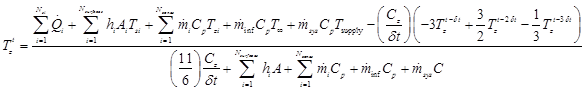
\includegraphics[width=0.9\textwidth, height=0.9\textheight, keepaspectratio=true]{media/image001.png}
\caption{EnergyPlus -- the big picture \protect \label{fig:energyplus-the-big-picture}}
\end{figure}

\textbf{\emph{Integration of Loads, Systems, and Plants:}} One of the strong points of EnergyPlus is the integration of all aspects of the simulation---loads, systems, and plants. Based on a research version of the BLAST program called IBLAST, system and plant output is allowed to directly impact the building thermal response rather than calculating all loads first, then simulating systems and plants. The simulation is coupled allowing the designer to more accurately investigate the effect of undersizing fans and equipment and what impact that might have on the thermal comfort of occupants within the building. The diagram below shows a basic overview of the integration of these important elements of a building energy simulation.

\begin{figure}[hbtp] % fig 2
\centering
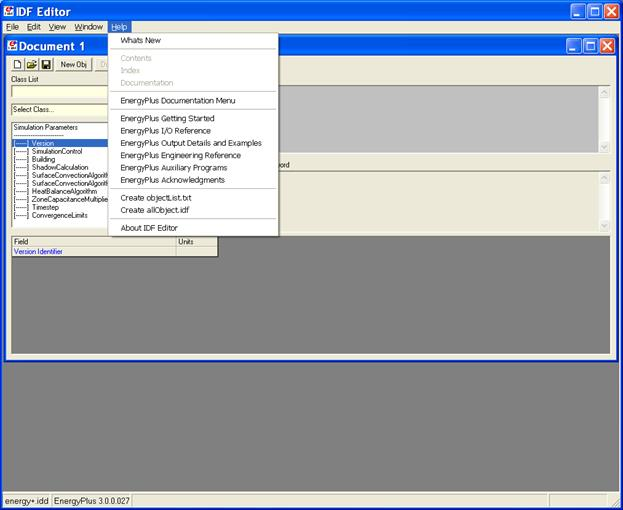
\includegraphics[width=0.9\textwidth, height=0.9\textheight, keepaspectratio=true]{media/image002.jpg}
\caption{EnergyPlus -- Internal elements \protect \label{fig:energyplus-internal-elements}}
\end{figure}

\textbf{\emph{``Open'' Source Code:}} Another advantage of EnergyPlus that it shares with both BLAST and DOE--2 is that the source code of the program will be available and open for public inspection, revision, etc. The program is not intended to be a black box that is unintelligible to the users and developers around the world. While there are many conflicting ideas on what is meant by ``open'', EnergyPlus is certainly not closed since this would be counter to the goals that have already been stated. The hope is that this access to source code will improve the accuracy and usability of the program over the long term and allow many developers to work on the program simultaneously. This ``developer friendly'' stance is critical to keeping EnergyPlus current and in step with technological advances.

In summary, the goals of EnergyPlus are ambitious but achievable via the path described above. EnergyPlus aims to be a program that is relatively simple to work with from the perspective of both the users and the developer. The development team made tremendous efforts to keep simulation code and algorithms as separate as possible and as modular as possible to minimize the overall knowledge that someone would need to have to add models to the program. This will minimize the resource investment and maximize the impact of current research in the field of building energy analysis and thermal load calculations. Finally, the full coupling of building envelopes, systems, and plants will provide a better understanding of how a building responds not only to the environmental factors that impact the building but also the HVAC system as it attempts to meet the thermal loads on the building.

It is also important to note that testing and verification are key issues in the development of any new program such as EnergyPlus. While there are large sections of EnergyPlus that consist of brand new code, the majority of the heat balance code can be traced back to the original parent programs. It should be noted that while this code has been significantly reengineered the team used what has been termed an ``evolutionary reengineering'' (ER) process. In ER, program code is modified stepwise in an effort to restructure it, modularize it, replace old obsolete data structures, etc. The ultimate goal is to bring it up to current programming standards without starting over with new code. At each step along the way, the program is exercised over a variety of input files and parameters to insure that what were intended to be algorithm neutral changes in the program have not resulted in changes to the output. This process was very successful and bolstered confidence in the program. In addition, comparisons could be made back to legacy programs to show that the new program is at a minimum as accurate as its predecessors. Beyond this, EnergyPlus has also been subjected to a lengthy and rigorous testing plan by an outside agency as well as numerous beta testers. This level of effort and collaboration is unprecedented in the history of energy analysis and thermal load calculation programs and has resulted in a much higher level of confidence in the results produced by EnergyPlus.


\section{EnergyPlus Documentation Library}\label{energyplus-documentation-library}

The documentation library for EnergyPlus has historically been provided in the form of pdf's packaged with the release. As of the 8.3.0 release, a major conversion was completed where the source of the docs was changed to Markdown. This allows for numerous improvements:

\begin{itemize}
\tightlist
\item
  Easy to automatically translate in between other markup languages, including html, thus making it easy to host as a web page.
\item
  Merging can be done automatically so the documentation source can stay alongside the source code, idd, and idfs, and all be merged at once. With the ever-increasing visibility of EnergyPlus development, it is becoming key that documentation is directly in sync with the rest of the program files.
\item
  Since Markdown is clear text, it is platform-independent and maximizes the possibility for outside contributions to EnergyPlus.
\end{itemize}

The Markdown source for the latest major release is converted to html which is then available at \url{http://energyplus.net/documentation}. The current, or ``daily'' documentation is available at \url{http://nrel.github.io/EnergyPlus}, but since this is a moving target within a release cycle, it is recommended that users view the .net documentation page.

Two key aspects of the documentation that are currently in development and should be completed soon are:

\begin{itemize}
\tightlist
\item
  Search: the ability to search the online html docs easily
\item
  Download as pdf: the ability to download pdfs for local/offline access
\end{itemize}

The Markdown based documentation is structured similarly to the pdfs, though the larger files are broken into smaller pieces for faster load times due to the dynamic nature of the math, especially in the engineering reference. Each of the main documentation pieces are described here.

\subsection{User Information Documents}\label{user-information-documents}

The following documents relate to using EnergyPlus, the engine. These documents cover a full range of questions and should be the first place a beginning or even experienced user would go to find out how the program works, what it expects as input, what it produces as output, etc. In general, the information in these documents is not highly technical, but it is detailed enough to use the basic capabilities of the program.

\textbf{\emph{Getting Started with EnergyPlus -- the Basics Manual:}} You are currently reading the Overview section of this document. The overview contains a ``big picture'' description of the EnergyPlus program as well as background of its development and the goals to which it ascribes. The remainder of the Getting Started document provides beginning users with an introduction into how to run EnergyPlus, what files are needed for EnergyPlus to execute, and what files are produced when EnergyPlus runs successfully. It also provides some guidance as to how to determine what potential sources of errors are when EnergyPlus runs into problems and how serious those problems might be.

\textbf{\emph{Input and Output Reference:}} This document is a thorough description of the various input and output files related to EnergyPlus, the format of these files, and how the files interact and interrelate.

\textbf{\emph{Output Details, Examples and Data Sets:}} While the Input and Output Reference document touch on some of the outputs from EnergyPlus, this document has more details and specific examples. It also addresses the reference data sets that are included.

\textbf{\emph{Auxiliary Programs}:}~This document contains information for the auxiliary programs that are part of the EnergyPlus package. For example, this document contains the user manual for the Weather Converter program, descriptions on using Ground Heat Transfer auxiliary programs with EnergyPlus, Compact HVAC descriptions, the Transition program/package and other assorted documents.

\subsection{Engineering Reference Document}\label{engineering-reference-document}

The Engineering Reference provides more in-depth knowledge into the theoretical basis behind the various calculations contained in the program. This reference includes more information on modeling equations, limitations, literature references, etc. The document contains the following information and is structured along the lines of the above illustration (Figure~\ref{fig:energyplus-internal-elements}. EnergyPlus -- Internal elements).

\textbf{\emph{Heat Balance Overview and Reference:}}~ This section describes the heat balance calculations that form the basis of the EnergyPlus building model. It includes descriptions of shadowing calculations and other pieces of the model.

\textbf{\emph{HVAC Overview and Reference:}}This section contains a description of the loop-based approach used by EnergyPlus to model the HVAC systems: air loops, water loops, etc. It includes a description of the higher-level managers that control the simulation flow as well as some information on the various components that can be linked together to comprise an HVAC system.

\textbf{\emph{HVAC Branch Based Input Description:}}This section is a special extension of both the input document and the HVAC overview document. It contains more detail on the various HVAC input objects and how these different object link together to form an HVAC description. It contains vital information mainly for the interface developer but also provides users with an in-depth look at the inner workings of the loop approach adopted by EnergyPlus.

\textbf{\emph{Encyclopedic Reference:}}If the information did not fit in the above categories, then the last part of the Engineering Reference is a detailed description of the various models.

\subsection{Application Guides}\label{application-guides}

The application guides are intended to address specific applications using EnergyPlus where the other documents may not provide cohesive examples of intended usage; that is, the techniques for doing certain things may be spread throughout other documents but warrant a more ``how to'' approach that will be present in these documents. The application guides are intended to become more prolific over time, specifically targeted to questions users have sent to the helpdesk support site.

\textbf{\emph{Current Application Guides:}}

\textbf{\emph{EMS Application Guide:}} This guide contains information useful to use the advanced feature of EnergyPlus: Energy Management System tweaks. The Erl language is described and examples for use are given.

\textbf{\emph{External Interface Application Guide:}} This guide contains information specific to using the external interface feature of EnergyPlus to connect other simulation systems.

\textbf{\emph{Plant Application Guide:}} This guide details the methods for simulating real chilled and hot water plant systems within EnergyPlus.

\textbf{\emph{Using EnergyPlus for Compliance Guide:}} This guide contains information specific to using EnergyPlus in Compliance and Standard Rating systems.

\textbf{\emph{External Interface(s) Application Guide:}} This guide contains information about external interfaces (through the Building Controls Virtual Test Bed link) to EnergyPlus.

\textbf{\emph{Tips \& Tricks for Using EnergyPlus:}} This guide contains short tips and tricks for using various parts of EnergyPlus.

\subsection{Developer Menu and Developer Information Documents}\label{developer-menu-and-developer-information-documents}

The following documents will be most useful to potential developers of EnergyPlus, both Interface Developers and Module Developers. Interface Developers will be creating input and output wraps on EnergyPlus so that is it is usable to the architect, design engineers, and others. Module developers will be creating new modules within the EnergyPlus structure and framework.

\textbf{\emph{Interface Developer's Guide:}} This document is critically important to persons interested in developing an interface that provides input to and read output from EnergyPlus. It is a comprehensive guide to the input data dictionary and the input data files that contain a user's building data. Each piece of input syntax is described in detail. In addition, the mechanism for obtaining output and the format in which output will be produced are discussed. This document also contains sections on weather files and units. Numerous samples and examples are given throughout the document with a full file length example provided in the appendix.

\textbf{\emph{Module Developer's Guide:}} This document contains a wealth of information that is intended to provide as much assistance as possible to persons interested in adding modules to the EnergyPlus program. It reviews the module concept as outlined in the programming standard and how they have been implemented in EnergyPlus. It provides a description of how the various modules work together and how the program is structured from a module tree (inverted tree) perspective. One of the most important features of this document is a list of standard EnergyPlus service subroutines and modules that greatly simplify the developers' task of integrating their work into the program. Input and output issues are also addressed from the perspective of how modules actually obtain data from the input file and how each section of the code sends data to the output files.


\chapter{Getting Started with EnergyPlus}\label{getting-started-with-energyplus}

The remainder of this document is intended to give you a start on using the program with a few simple tools (EP-Launch to help run the simulation; IDFEditor to help create or look at input files) as well as some of the features (such as energy meters, simulation results) of using the program.

For learning about a specific input file, or a specific input object, the install includes two documents in the ExampleFiles folder:

\begin{itemize}
\item
  Example Files Summary (highlights of each example file)
\item
  Example Files Links to Objects (for any object, up to 3 files using that object are shown)
\end{itemize}

The standard Windows install procedure has put the following information on your computer, in the directories/folders shown.

The main EnergyPlus folder contains: * Energy+.idd * EnergyPlus.exe and dependent shared libraries (dll files) * RunEPlus.bat and other batch files for running EnergyPlus * readme file(s), license, etc. * EP-Macro.exe and other support binaries * bugreprt.txt~

The general layout of folders from the install looks like:

\begin{lstlisting}
. EnergyPlus main folder
+-- Documentation
|   +-- A link to find the documentation online, and any additional docs packaged with the installation
+-- DataSets
|   +-- Reference Data Sets (libraries)
+-- MacroDataSets
|   +-- Macroized Reference Data Sets (libraries)
+-- PreProcess
|   +-- FMUParser              Tool for external interface specific applications
|   +-- IDFEditor              Program files for the IDFEditor
|   +-- GrndTempCalc           Special program to calculate ground temperatures.
|   +-- DOE2Translator         Simple translator for DOE-2 files
|   +-- WeatherConverter       Tool for performing weather file creation and conversion
|   +-- ParametricPreprocessor Parametric simulation tool
|   +-- IDFVersionUpdater      Graphical tool for updating old EnergyPlus files to the latest version
+-- PostProcess
|   +-- ReadVarsEso            The simple post processor exe.
|   +-- EPCompare              A graphical tool for comparing two EnergyPlus output sets
+-- ExampleFiles               Sample input, output, results files shipped with the program.
+-- WeatherData                Sample weather files shipped with the program.
\end{lstlisting}


\chapter{Running EnergyPlus}\label{running-energyplus}

EnergyPlus is written in C++ and runs as a console application. More explicit details on running EnergyPlus are available in a separate document (Running EnergyPlus in Auxiliary Programs document). Optional command-line arguments are available (energyplus --help, or man energyplus on Linux systems). The following files are used to run EnergyPlus:

\begin{itemize}
\item
  EnergyPlus.exe (the executable file)
\item
  Energy+.ini (described below)
\item
  Energy+.idd (the input data dictionary file)
\item
  In.idf (the input file)
\item
  In.epw -- optional (weather data file)
\end{itemize}

The input data dictionary and input data file have been discussed in the previous sections of this document.

For weather simulations, EnergyPlus accepts EnergyPlus weather files. Previous versions accepted BLAST formatted weather files and now a BLASTWeatherConverter program is provided.~ The actual file name is \textbf{in.epw}.

The Energy+.ini file is a ``standard'' Windows™ ini file and can be manipulated using the Windows API calls though EnergyPlus uses standard Fortran to manipulate it.~ It is a very simple ini file and is fully described in the \href{file:///E:/Docs4PDFs/AuxiliaryPrograms.pdf}{Auxiliary Programs} document. Energy+.ini and in.idf file should be in the directory from which you are running EnergyPlus.exe.

For the advanced user, there is also the ``EPMacro'' program, described in the Auxiliary Programs Document.~ You run it as a separate program before EnergyPlus (the batch file included in the install and shown in the GettingStarted document contains the commands).

EnergyPlus creates the following files (plus more):

% table 2
\begin{longtable}[c]{@{}ll@{}}
\caption{EnergyPlus Output Files \label{table:energyplus-output-files}} \tabularnewline
\toprule 
FileName & Description \tabularnewline
\midrule
\endfirsthead

\caption[]{EnergyPlus Output Files} \tabularnewline
\toprule 
FileName & Description \tabularnewline
\midrule
\endhead

Audit.out & Echo of input \tabularnewline
Eplusout.err & Error file \tabularnewline
Eplusout.eso & Standard Output File \tabularnewline
Eplusout.eio & One time output file \tabularnewline
Eplusout.rdd & Report Variable Data Dictionary \tabularnewline
Eplusout.dxf & DXF (from Report,Surfaces,DXF;) \tabularnewline
Eplusout.end & A one line summary of success or failure \tabularnewline
\bottomrule
\end{longtable}

The eplusout.err file may contain three levels of errors (Warning, Severe, Fatal) as well as the possibility of just message lines.~ These errors may be duplicated in other files (such as the standard output file).

% table 3
\begin{longtable}[c]{@{}ll@{}}
\caption{EnergyPlus Errors \label{table:energyplus-errors}} \tabularnewline
\toprule 
Error Level & Action \tabularnewline
\midrule
\endfirsthead

\caption[]{EnergyPlus Errors} \tabularnewline
\toprule 
Error Level & Action \tabularnewline
\midrule
\endhead

Warning & Take note \tabularnewline
Severe & Should Fix \tabularnewline
Fatal & Program will abort \tabularnewline
\bottomrule
\end{longtable}

EnergyPlus produces several messages as it is executing, as a guide to its progress.~ For example, the run of the 1ZoneUncontrolled input file from Appendix A produces:

\begin{lstlisting}

EnergyPlus Starting
   EnergyPlus 1.3.0.011, 4/5/2006 2:59 PM
   Initializing New Environment Parameters
   Warming up {1}
   Initializing Response Factors
   Initializing Window Optical Properties
   Initializing Solar Calculations
   Initializing HVAC
   Warming up {2}
   Warming up {3}
   Warming up {4}
   Starting Simulation at 12/21 for DENVER_STAPLETON ANN HTG 99% CONDNS DB
   Initializing New Environment Parameters
   Warming up {1}
   Warming up {2}
   Warming up {3}
   Starting Simulation at 07/21 for DENVER_STAPLETON ANN CLG 1% CONDNS DB = >MWB
   EnergyPlus Run Time = 00hr 00min  1.00sec
\end{lstlisting}

Extensive timing studies and fine-tuning of EnergyPlus is NOT complete.~ To give you an idea of comparable run times, we present the following (does not include HVAC) with an early version of EnergyPlus running on a 450MHZ machine.~ Remember, BLAST would be 1 calculation per hour, EnergyPlus (in this case) was 4 calculations per hour.~ Obviously, these are quite out of date.~ However, a recent change in a developer's test machine illustrates the importance of maximum memory.~ A 5 zone full year run on a 1.8GHZ, 1GB machine was running about 8 minutes -- with a new 2.1GHZ, 2GB machine the same file takes about 2 minutes.

% table 4
\begin{longtable}[c]{p{3.0in}p{1.5in}p{1.5in}}
\caption{Timings Comparison (EnergyPlus vs. BLAST) \label{table:timings-comparison-energyplus-vs.-blast}} \tabularnewline
\toprule 
File & BLAST Per Zone & EnergyPlus Per Zone \tabularnewline
\midrule
\endfirsthead

\caption[]{Timings Comparison (EnergyPlus vs. BLAST)} \tabularnewline
\toprule 
File & BLAST Per Zone & EnergyPlus Per Zone \tabularnewline
\midrule
\endhead

GeometryTest (5 Zones, 2 Design Day, Full Weather Year) & 13 sec & 33 sec \tabularnewline
SolarShadingTest (9 Zones, Full Weather Year) & 7 sec & 25 sec \tabularnewline
\bottomrule
\end{longtable}


\chapter{Introduction}\label{introduction}

EnergyPlus is a modular simulation program designed to model the performance, energy consumption and pollutant production of a building. EnergyPlus models energy transport through the building envelope, heat gains within the building, and all the HVAC equipment used to heat and cool the building. The program is designed for ease of development. The concept is that many people will contribute to EnergyPlus and the program structure has been designed to make this possible.

EnergyPlus is written entirely in Fortran 90 with updates to Fortran 95 -- all of EnergyPlus code should be at minimum Fortran 90 compliant and can accept the newer features of Fortran 95 as well. Fortran 90/95 is a powerful modern programming language with many features. Using Fortran 90/95 it is possible to program in many different styles. The EnergyPlus team has chosen a particular style that emphasizes code extensibility (ease of development), understandability, maintainability, and robustness. Less emphasis was placed on program speed and size. Fortran 90/95 has all the features that permit the creation of readable, maintainable, and extensible code. In particular, the ability to create data and program modules with various levels of data hiding allows EnergyPlus to be built out of semi-independent modules. This allows a new EnergyPlus developer to concentrate on programming a single component without having to learn the entire program and data structure.

The EnergyPlus programming style is described in the \emph{EnergyPlus Programming Standard.} The \emph{Programming Standard} should be consulted for details such as variable and subroutine naming conventions. In this document, we will describe the steps a developer must follow to create a new EnergyPlus component model. In particular, we will assume the developer wishes to simulate an HVAC component that cannot yet be modeled by EnergyPlus.


\section{EP-Launch Program}\label{ep-launch-program}

EP-Launch is an optional component of the EnergyPlus Windows installation (it is not available for Linux and Mac platforms). For users that want a simple way of selecting files and running EnergyPlus, EP-Launch provides this and more. In addition, EP-Launch can help open a text editor for the input and output files, open a spreadsheet for the postprocessor results files, a web browser for the tabular results file, and start up a viewer for the selected drawing file.

\begin{figure}[hbtp] % fig 4
\centering
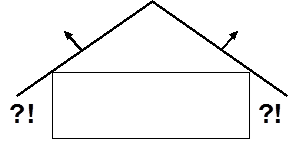
\includegraphics[width=0.9\textwidth, height=0.9\textheight, keepaspectratio=true]{media/image004.png}
\caption{EP-Launch Screen \protect \label{fig:ep-launch-screen}}
\end{figure}

\subsection{Start EP-Launch}\label{start-ep-launch}

EP-Launch is located in the main directory/folder for EnergyPlus. In addition, it is available on the shortcut menu for EnergyPlus.~ By double clicking on the EP-Launch icon you get the screen shown above (Figure~\ref{fig:ep-launch-screen}) for running a single input file. The EP-Launch program simply starts other programs and allows you to avoid having to use the DOS command line prompt to run EnergyPlus. More help is provided for the program under the ``Help'' menu.

\subsection{Selecting Input and Weather Files}\label{selecting-input-and-weather-files}

The input file and weather files can be selected on the Single Input File tab from the two pull down lists which show recently used files or you can press the ``Browse\ldots{}'' buttons to locate an input or weather file that you have created yourself. If this is your first time using EP-Launch, the pull down lists will show some files from the ExampleFiles subdirectory. These are not the only examples, use browse to open other example files from the ExampleFiles subdirectory or other EnergyPlus input files.

\subsection{Running a Single Input File}\label{running-a-single-input-file}

On the Single Input File tab, after you select the weather and input files simply push the ``Simulate\ldots{}'' button to start the EnergyPlus building energy simulation engine. At this point a black DOS window should pop up on your screen and show the progress of your simulation. The simulation is complete when the black DOS box closes. The EnergyPlus program black DOS window will show scrolling text as the simulation procedure progresses. If you would like to see these messages more slowly you have two options:

1)~~~Press the ``Control-S'' key combination to try to stop the progress and any key to continue.

2)~~~Under the ``View'' menu on the EP-Launch program, select ``Options'' then ``Command Window'' then check ``Pause During Simulation'' and this will pause the process immediately after EnergyPlus executes. To continue after the pause, press any key.

If the file contains Parametric objects, the single input file may cause multiple simulations to be performed. If multiple simulations are performed, the output files will be listed on the History tab and will be named with either the file suffixes defined in the input file or with a serial number.

Multiple single input file and group simulations can be started at the same time. On a computer with multiple-processors or multiple-cores, this will enable the simulations to complete more quickly than starting one after another.

\subsection{Looking at the Results}\label{looking-at-the-results}

After you have run a simulation and the black DOS window closes, EnergyPlus has completed, and a status message is displayed see Figure~\ref{fig:ep-launch-finish-status}:

\begin{figure}[hbtp] % fig 5
\centering
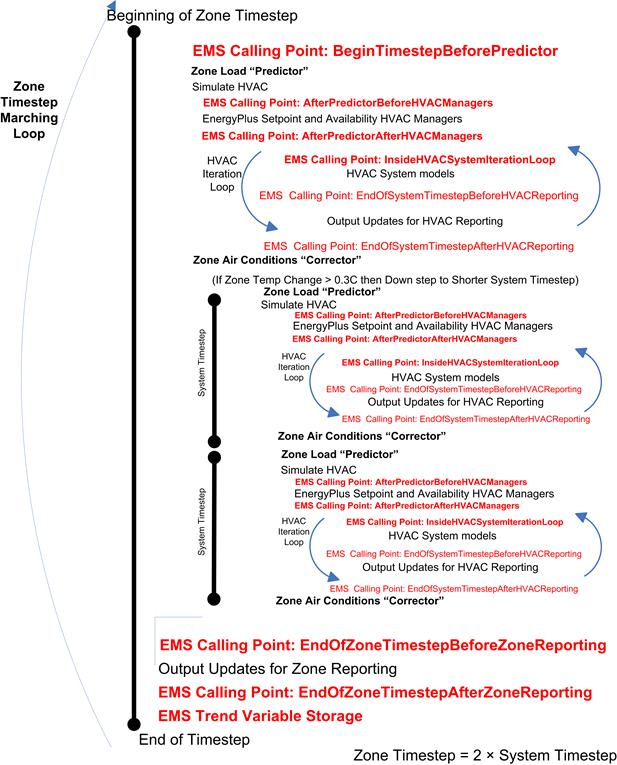
\includegraphics[width=0.9\textwidth, height=0.9\textheight, keepaspectratio=true]{media/image005.jpg}
\caption{EP-Launch Finish Status \protect \label{fig:ep-launch-finish-status}}
\end{figure}

This status gives you a quick overview of whether there were warning (\textbf{should look at}), severe (\textbf{should probably fix}) or fatal (\textbf{must fix}) errors in the run as well as the time it took for the simulation to complete.~ After pressing ``OK'' from this box, selecting ``ERR/EIO/BND Output Files Only'' from the ``View'' menu will display the ERR, EIO, and BND files -- useful when errors may have occurred. Alternatively, pressing the F2 function key will display the same three files.

Another way to open files easily is by using the View Results buttons shown in Figure~\ref{fig:ep-launch-with-the-sets-tab-of-view-results}. Two different panels of buttons can be used under View Results, one shown by using the ``All'' tab on the left edge and by using the ``Sets'' tab on the left edge. The ``All'' tab shows all the various files by file extension that can be viewed individually.~ Files available for view~ based on the current input file name are ``enabled'' (extension names clearly readable). The contents of each file extension is listed below.

\begin{figure}[hbtp] % fig 6
\centering
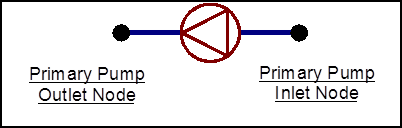
\includegraphics[width=0.9\textwidth, height=0.9\textheight, keepaspectratio=true]{media/image006.png}
\caption{EP-Launch with the Sets tab of View Results \protect \label{fig:ep-launch-with-the-sets-tab-of-view-results}}
\end{figure}

The figure above shows the same main screen of EP-Launch but with the ``Sets'' tab selected on the left edge of the View Results section. The buttons on this tab can open many files at the same time and are a shortcut to opening the files that may be commonly used. The Text Output Files, Drawing Files, and Spreadsheets buttons cause several different results files to open at once based on the currently selected Input File. The HTML file opens just the tabular results file if that file was produced (see \emph{OutputContol:Table:Style}).

The contents (along with examples) are discussed in the \href{file:///E:/Docs4PDFs/OutputDetailsAndExamples.pdf}{Output Details} document.

You can also view the results using one of the three buttons (``Text Output Files,'' ``Drawing File'' and ``Spreadsheets'') in the ``View Results'' area of the main EP-Launch screen.

By pressing the ``Text Output Files'' button, a text editor will open each of the text output files. Up to 29 files will open, if they exist. Selecting ``Single File'' from the `View `` menu displays a menu of all available output files from which any file can be opened individually. Each file may also be opened with an associated function key. The output files and function key shortcuts are listed below:

1.~Variable -- tabulated results in comma, tab or space delimited format (generated by the ReadVarsESO postprocessor) (F4)

2.~ESO -- raw report variable output (F5),

3.~RDD -- list of output variables available from the run (F6).

4.~MDD -- list of output meters available from the run (Shift-Ctrl-F3)

5.~EIO -- additional EnergyPlus results (F7),

6.~ERR -- list of errors and warnings (F8),

7.~BND -- HVAC system node and component connection details (F9),

8.~MTR -- raw report meter output (F11),

9.~MTD -- list of meter component variables (F12)

10.~METER File -- tabulated meter report in comma, tab or space delimited format (generated by the ReadVarsESO postprocessor) (Ctrl-F4)

11.~ZSZ -- zone sizing details in comma, tab or space delimited format (Ctrl+F5)

12.~SSZ -- system sizing details in comma, tab or space delimited format (Ctrl+F6)

13.~AUDIT -- input file echo with input processor errors and warnings (Ctrl+F8)

14.~SLN -- output from ``report, surfaces, lines'' (Ctrl+F9)

15.~DBG -- output from the debug command (Ctrl+F11)

16.~SHD -- output related to shading (Ctrl+F12)

17.~SVG - HVAC Diagram (Shift+ F4)

18.~EPMIDF -- clean idf file after EP-Macro processing (Shift+F5)

19.~EPMDET -- EP-Macro detailed output with errors and warnings (Shift+F6)

20.~MAP -- daylighting illuminance map (Shift+F7)

21.~TABLE -- tabulated report of bin and monthly data in comma, tab or space delimited or HTML format~ (Shift+F8)

22.~VMRL -- drawing file in VRML (Virtual Reality Markup Language) format (Shift F+F11)

23.~DXF -- drawing file in AutoCAD DXF format (Shift+F12)

24.~Delight IN - DElight input generated from EnergyPlus processed input (Shift+Ctrl+F4)

25.~Delight OUT -- Detailed DElight output (Shift+Ctrl+F5)

26.~Delight ELDMP -- DElight reference point illuminance per time step (Shift+Ctrl+F6)

27.~Delight DFDMP -- DElight warning and error messages (Shift+Ctrl+F7)

28.~EXPIDF -- Expanded IDF when using HVACTemplate objects (Shift+Ctrl+F8)

29.~Group Error -- combined error files for a group run. (Shift+Ctrl+F9)

30.~VCpErr -- Transition program error file (Shift+Ctrl+F11)

31.~Screen (Shift+Ctrl+f12)

32.~Proc CSV -- Simple statistiscs generated from CSVProc (also see Create Statistics File option under View-Options).

33.~EDD -- Energy Management System details.

Clicking on the ``Drawing File'' button will open the generated DXF file if an appropriate viewer has been configured (see \emph{Selecting Viewers and Editors} below). The DXF file is a CAD format that displays the physical shape of the building being modeled in three dimensions. The ``Drawing File'' button also opens the HVAC diagram generated with the HVAC-Diagram utility (see Auxiliary Programs).

Clicking on the ``Spreadsheets'' buttons will open any generated CSV files if an appropriate viewer has been configured (see \emph{Selecting Viewers and Editors} below).

\subsection{Viewing the Drawing File without Running a Simulation}\label{viewing-the-drawing-file-without-running-a-simulation}

The ``Drawing'' button (or the View menu Drawing File option) will automatically run EPDrawGUI if the DXF file does not exist or it is older than the input file. This allows the building geometry to be viewed without running a full simulation. For more information about EPDrawGUI, see the \href{file:///E:/Docs4PDFs/AuxiliaryPrograms.pdf}{\emph{Auxiliary Programs}} document.

\subsection{Editing the Input Files}\label{editing-the-input-files}

The input file, called IDF file that is selected from the top pull-down list, can be edited by pressing one of two buttons in the ``Input File'' area. The ``Edit - Text Editor'' button will start a text editor and the ``Edit - IDF Editor'' will start the separate program called the IDF Editor. Remember to save any changes you make in either editor before returning to EP-Launch to run the simulations again.

\subsection{File Menu}\label{file-menu}

The File menu can be used for selecting input and weather files just like the ``Browse\ldots{}'' buttons (see the \emph{Selecting Input and Weather Files} section above).

If you are upgrading from the previous version of EnergyPlus you can use the ``File'', ``Transition'' menu option to upgrade your EnergyPlus input files (IDF and IMF) to the most recent version (see the \href{file:///E:/Docs4PDFs/AuxiliaryPrograms.pdf}{AuxiliaryPrograms} document for more information about the Transition program). This EP-Launch option only works for upgrading input files one version.

\subsection{Edit Menu}\label{edit-menu}

No cutting or pasting is used in this program so the edit menu shows options that duplicate the functions of the ``Edit -- Text Editor'' and ``Edit -- IDF Editor'' buttons. In addition, the weather file and the postprocessor command file (rvi) may be opened in the text editor.

\subsection{View Menu}\label{view-menu}

The View menu (Figure~\ref{fig:ep-launch-view-menu}) duplicates the options in the ``View Results'' area of the main screen (see the \emph{Looking at the Results} section above) and allows opening of selected output files. You can also open the folders that contain the active input and weather files. Opening a single file is under a submenu and is very similar to the Quick Open Panel for Single Simulation described above. Selecting ``HTML File'' from the ``View'' menu will open any user created files saved in the format: \textless{}filename\textgreater{}table.html (see \emph{OutputControl:Table:Style}).

\begin{figure}[hbtp] % fig 7
\centering
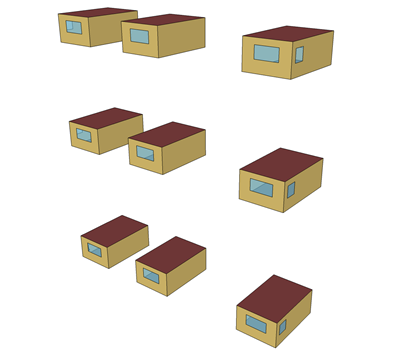
\includegraphics[width=0.9\textwidth, height=0.9\textheight, keepaspectratio=true]{media/image007.png}
\caption{EP-Launch View Menu \protect \label{fig:ep-launch-view-menu}}
\end{figure}

\begin{figure}[hbtp] % fig 8
\centering
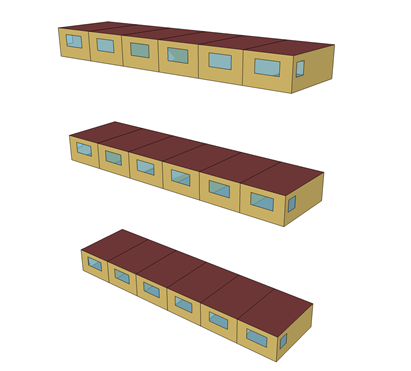
\includegraphics[width=0.9\textwidth, height=0.9\textheight, keepaspectratio=true]{media/image008.png}
\caption{EP-Launch Options Screen. \protect \label{fig:ep-launch-options-screen.}}
\end{figure}

The ``View'' menu also accesses the ``Options'' menu item shown in Figure~\ref{fig:ep-launch-options-screen.} that is used to control many of the optional features of EP-Launch. These optional features are described below:

\subsubsection{Command Window Options}\label{command-window-options}

\textbf{Pause During Simulation (Unless Minimized)} -- Stops the progress of the EnergyPlus run at different points. This does not stop the simulation itself but pauses before or after important events as files are copied or utility programs are run. It is usually used only for diagnosing problems with the EPL-RUN batch file. The feature is also described in the \emph{Running a Single Input File} section above.

\textbf{Minimize Single Simulation Command Window} -- For a single input file, minimizes the Command Window that EP-Launch uses to run EnergyPlus. The command window will appear only in the Windows taskbar and the command window will not be visible. You can restore the command window be clicking on the taskbar item labeled ``EnergyPlus Process''. This option should be used with caution since you will not see any indication of the simulation being complete other than the ``EnergyPlus Process'' taskbar item will disappear.

\textbf{Minimize Group Simulation Command Window} -- For a group of input files, minimizes the Command Window that EP-Launch uses to run EnergyPlus. This is a good option when working on something else on your computer at the same time as the group of simulations is running since the command window normally becomes the front window each time a new simulation starts. This option prevents the command window coming to the front for each simulation. The command window will appear only in the Windows taskbar and the command window will not be visible. You can restore the command window be clicking on the taskbar item labeled ``EnergyPlus Process''. This option should be used with caution since you will not see any indication of the simulation being complete other than the ``EnergyPlus Process'' taskbar item will not be present.

\textbf{Number of Simultaneous Processes} -- Select the maximum number of simulations that should be able to be run at the same time. For a computer with multiple processors or multiple cores, this will allow better utilization of the computers power. The value selected should correspond to the number of processors/cores but higher or lower number can be used as well.

\subsubsection{Interface Options}\label{interface-options}

\textbf{Extra Wide Window} -- Select this option to make the main EP-Launch window wider. This is useful when files are used with very long file path names.

\textbf{Alternative layout} -- Changes the layout of the EP-Launch window to an alternative arrangement of buttons.

\subsubsection{Miscellaneous Options}\label{miscellaneous-options}

\textbf{Tab Delimited Open with Spreadsheet} -- Selecting ''Single File'' and then ``Main Results File'' from the ``View'' menu or pressing the F4 function key will open TAB files with the default spreadsheet application rather than the text editor. Comma-separated variable (CSV) is the default setting for viewing tabulated results set in the RVI file. If the user changes the setting for viewing tabulated results to TAB or TXT format, selecting ''Single File'' and then ``Main Results File'' from the ``View'' menu or pressing the F4 function key will open the files in the default text editor.~ TAB files, when selected, will also be opened by the text editor when the ``Text Output Files'' button is pressed after a successful run.

\textbf{Allow More Than 250 Columns} -- Tabulated data that exceeds 250 columns, the MS Excel maximum, will be truncated to that limit unless ``Allow \textgreater{}250 Columns'' is selected. Excel versions prior to 2007 were limited to 255 columns in a sheet; later versions allow unlimited number of columns. This limitation may not be true for other spreadsheet programs.

\textbf{Check VERSION Prior to Simulation} -- Automatically check the VERSION object in the selected EnergyPlus input file prior to simulation and if it is an older version than the current version will run the Transition program to update the file.

\textbf{Convert ESO/MTR to IP Units} -- Runs the convertESOMTR utility program (see AuxiliaryPrograms documentation for more information). This utility will convert the ESO and MTR files into Inch-Pound units. The CSV file created from these files will also be in Inch-Pound units.

\textbf{Create Statistics File} -- Runs the CSVProc utility program (see the AuxiliaryPrograms documentation for more information) and creates the --Proc.csv file. This file contains some simple statistics on each variable in the normal CSV file.

\textbf{Create Batch File to Run EnergyPlus} -- Traditionally EP-Launch has created a batch file in order to execute EnergyPlus with the various options chosen. This can cause problems with some operating systems, such as Windows Vista, when set to a higher security setting.~ This option can be unchecked and a batch file is not created when running EnergyPlus instead parameters are passed to an existing batch file.

\textbf{Run ParametricPreprocessor} -- When this option is checked, if Parametric objects are present in the file, the ParametricPreprocessor will be run prior to the first simulation and if multiple simulations are needed they will all be executed. See the Auxiliary Programs documentation for details.

\textbf{Check for Updates to EnergyPlus} -- When this option is checked, EP-Launch will check every seven days if an update to EnergyPlus or any of the files distributed with EnergyPlus are available to download. If they are available a message will be shown upon start up.~ You can also manually check by going to HELP .. CHECK FOR UPDATES.

\subsubsection{Text Editor Options}\label{text-editor-options}

EP-Launch will start a text editor when editing a IDF file or when viewing many of the results files.~ The text editor that will be used is shown but can be changed by either pressing the Select button or by pressing the Auto Find button. The Select button allows you to find the text editor of your choice. The Auto Find button will automatically find the program that is associated with the TXT file extension and use that program. Auto Find is invoked the first time EP-Launch is started so that a text editor is available immediately. The most common text editor is NOTEPAD.EXE and is built into Windows but many other text editors are also available.

\subsubsection{Drawing Viewer Options}\label{drawing-viewer-options}

The default drawing viewer is the application associated with DXF files. This can be changed to your favorite drawing program by using the Select button then locating the executable file for your favorite drawing software capable of reading a DXF file. The Auto Find button will automatically find the program that is associated with the DXF file extension and use that program. A variety of programs (free of charge) can render DXF files for viewing.~ The \href{file:///E:/Docs4PDFs/OutputDetailsAndExamples.pdf}{Output Details} document lists some of these programs as well as displaying what a DXF rendered file looks like on the screen.

\subsubsection{VRML Viewer Options}\label{vrml-viewer-options}

EP-Launch will start a VRML Viewer when a building drawing is created using the Report, Surfaces, VRML option in your IDF file.~ The VRML Viewer that will be used is shown but can be changed by either pressing the Select button or by pressing the Auto Find button. The Select button allows you to find the VRML Viewer of your choice. The Auto Find button will automatically find the program that is associated with the WRL file extension and use that program. Auto Find is invoked the first time EP-Launch is started so that a VRML Viewer is available immediately. Many other VRML Viewers are available.

\subsubsection{Spreadsheet Options}\label{spreadsheet-options}

EP-Launch will start a spreadsheet program when viewing many of the results files.~ The spreadsheet that will be used is shown but can be changed by either pressing the Select button or by pressing the Auto Find button. The Select button allows you to find the spreadsheet program of your choice. The Auto Find button will automatically find the program that is associated with the CSV file extension and use that program. Auto Find is invoked the first time EP-Launch is started so that a spreadsheet program is available immediately.

\subsubsection{Diagramming Options}\label{diagramming-options}

EP-Launch will start a diagramming program to view SVG files from HVAC Diagram.~ The diagramming program that will be used is shown but can be changed by either pressing the Select button, the Auto Find button, the Use Firefox button or the Use Opera button. The Select button allows you to find the diagramming program of your choice but make sure it is capable of opening SVG files. The Auto Find button will automatically find the program that is associated with the SVG file extension and use that program. Auto Find is invoked the first time EP-Launch is started so that a spreadsheet program is available immediately.~ Since both Firefox and Opera web browsers can view SVG files, those buttons will select those respective browsers if available.

\subsubsection{HTML Browser Options}\label{html-browser-options}

EP-Launch will start a HTML browser program when viewing the tabular results file when HTML is chosen in OutputControl:Table:Style object. The HTML browser that will be used is shown but can be changed by either pressing the Select button or by pressing the Auto Find button. The Select button allows you to find the HTML browser of your choice. The Auto Find button will automatically find the program that is associated with the HTML file extension and use that program. Auto Find is invoked the first time EP-Launch is started so that a HTML browser is available immediately.

\subsubsection{ESO Viewer Options}\label{eso-viewer-options}

By default, ESO files are opened with a text editor. ESO files are the raw output file containing results from EnergyPlus for Output:Variable objects. They are often processed into CSV files to make it easier to view them. At least one utility program has been developed to view ESO files directly (see the EnergyPlus.gov web site under ``Interfaces \& Other Tools'', ``Third-party EnergyPlus Tools).~ The Auto Find and Select buttons work the same way as other viewer selectors. If no special ESO viewer is selected the box will be shown as empty. It can also be emptied by using the Clear button.

\subsubsection{PDF Viewer Options}\label{pdf-viewer-options}

EP-Launch will start a PDF viewer program when opening the EnergyPlus documentation under the Help menu.~ The PDF Viewer that will be used is shown but can be changed by either pressing the Select button or by pressing the Auto Find button. The Select button allows you to find the PDF Viewer of your choice. The Auto Find button will automatically find the program that is associated with the PDF file extension and use that program. Auto Find is invoked the first time EP-Launch is started so that a PDF Viewer is available immediately.

\subsubsection{File Association Options}\label{file-association-options}

When installing EnergyPlus, you are given an option if you want IDF, IMF, and EPG files associated with EP-Launch. This allows double clicking on files with those extensions and having EP-Launch start automatically with those files. If during the install that option is not selected or if you have changed the program that opens IDF, IMF and EPG files and want to change it back to EP-Launch, the button for this option will do that.

\subsubsection{Reset Options}\label{reset-options}

Two reset options are available here.

The \textbf{Auto Find All File Viewers} button will autofind all the file viewers in one step. This is equivalent to pressing the Auto Find button for each viewer program.

The \textbf{Reset All Options and Exit} button will clear all options and restore the default values used when first invoking EP-Launch for the first time. This also clears the list of recently used IDF and weather files.~ This option will exit EP-Launch and you will have to start EP-Launch again.

\subsection{Help Menu}\label{help-menu}

The Help menu can be used to open the EnergyPlus documentation files and the EP-Launch help file. In addition, you can check for updates to the EnergyPlus program and other files in the EnergyPlus distribution.

\subsection{Recently Used Files}\label{recently-used-files}

The recently used input, weather and group file pull down lists can hold a maximum of twenty items. These lists, like the viewers selected, are saved between times you use the EP-Launch program.

\subsection{Utilities Tab}\label{utilities-tab}

The utilities tab shown in the following figure allows several utility programs that come with EnergyPlus to be used directly. More information on each utility is also available in the AuxiliaryPrograms documentation.

\begin{figure}[hbtp] % fig 9
\centering
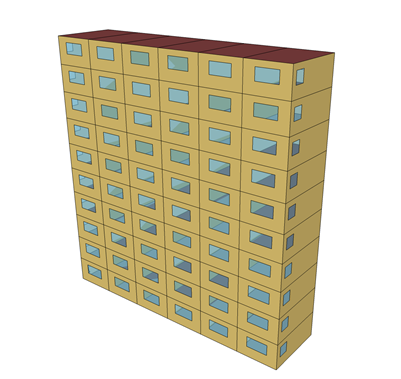
\includegraphics[width=0.9\textwidth, height=0.9\textheight, keepaspectratio=true]{media/image009.png}
\caption{EP-Launch Utilities Tab. \protect \label{fig:ep-launch-utilities-tab.}}
\end{figure}

For each utility, input files can be selected by using the Browse Button. The input file can be opened using a text editor and, for certain utilities, the IDF Editor. If a weather file is needed for a utility it can also be selected. For other utilities, no weather file is needed and that portion of the screen is not shown. The appropriate output files can be opened by the ``Open'' button near the bottom of the screen. To run the utility, use the ``Run'' button in the lower left corner of the screen above the ``Exit'' button.

In addition, for each utility, a brief description of the function of the utility is shown in the about box but much more information is available in the AuxiliaryPrograms documentation.

\subsection{Caveats}\label{caveats}

Remember to save changes made in the editor before you run another simulation.

The simulation cannot write new results to open files which are locked by another application.

You will need to close the spreadsheet program that views the resulting CSV files prior to another simulation and you may need to close the text editor windows also (depending on your editor).

The EPL-RUN.BAT batch file is used to run EnergyPlus from the EP-Launch program. It can be edited with care if other postprocessors or preprocessors are to be used.

\subsection{When things go wrong}\label{when-things-go-wrong}

Though EnergyPlus has had several releases (including beta releases prior to initial release), there still may be problems when input files meet with EnergyPlus. If you are using EP-Launch when this happens, you will see a window appear as in the figure below (Figure~\ref{fig:energyplus-crash-within-ep-launch.}). Follow the instructions listed on the screen.

\begin{figure}[hbtp] % fig 10
\centering
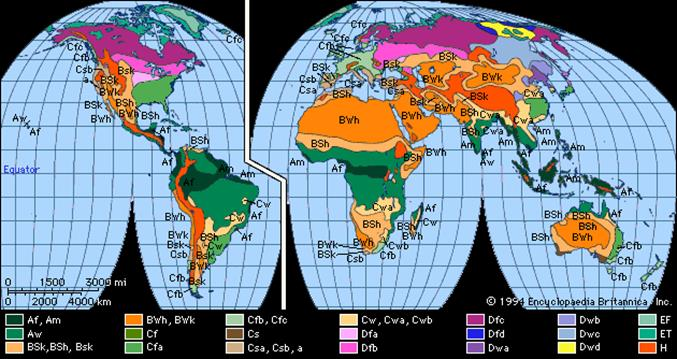
\includegraphics[width=0.9\textwidth, height=0.9\textheight, keepaspectratio=true]{media/image010.jpg}
\caption{EnergyPlus crash within EP-Launch. \protect \label{fig:energyplus-crash-within-ep-launch.}}
\end{figure}

\subsection{Bugs}\label{bugs}

The EP-Launch program has been through several ``releases'' but there is still a chance you will find bugs. Please report them to the energyplus-support@gard.com address so that we can fix them prior to the release.

If the pull-down lists ever are shown as blank the ``reset'' button may be used. This unlabeled button is very small in the lower left-hand corner of the main screen. It removes the items shown in the recently used file list and causes the program to forget the selected viewers and text editors; and exits the program. When you start EP-Launch again, you will need to make these selections (viewers and text editors) again.


\section{EnergyPlus File Extensions}\label{energyplus-file-extensions}

This section will present a list (perhaps not complete) of EnergyPlus file extensions and what they mean. This will help you after the EP-Launch program finishes.

\subsection{Input Files}\label{input-files}

The following files are input to the EnergyPlus program.

\subsubsection{IDD}\label{idd}

The \emph{input data dictionary} (IDD) is an ascii (text) file containing a list of all possible EnergyPlus objects and a specification of the data each object requires. This file is analogous to the DOE-2 keyword file. The \emph{Guide for Interface Developers} contains a full description of the input data dictionary.

\subsubsection{idf}\label{idf}

The \emph{input data file} (IDF) is an ascii file containing the data describing the building and HVAC system to be simulated. Many example files are installed as part of the EnergyPlus installation. Additionally, a spreadsheet file ``ExampleFiles.xls'' contains columnar descriptions of each file's features.

\subsubsection{imf}\label{imf}

The \emph{input macro file} (IMF) is an ascii file containing the data describing the building and HVAC system to be simulated and will have some contents of ``macro'' commands. The Auxiliary programs document describes use of the macro commands and the program that processes them - EP-Macro. Many example files are installed as part of the EnergyPlus installation.

\subsubsection{ini}\label{ini}

This is the EnergyPlus initialization file. It is an optional ascii input file that allows the user to specify the path for the directory containing Energy+.idd. This file, using the actual directories of the install, will be created during the install. Unless you change where the EnergyPlus.exe file resides, you will not need to change this file.

\subsubsection{epw}\label{epw}

The \emph{EnergyPlus weather} file is an ascii file containing the hourly or sub-hourly weather data needed by the simulation program. The data format is described in detail in the Auxiliary Programs Document. It is also described succinctly in the Input Output Reference document.

\subsection{Output Files}\label{output-files}

More information (and more up-to-date) about output files is shown in the \href{file:///E:/Docs4PDFs/OutputDetailsAndExamples.pdf}{Output Details and Examples} Document.

\subsubsection{err}\label{err}

A text file containing the error messages issued by EnergyPlus. \textbf{This is the first output that should be examined after a simulation.}Error messages may be issued by EnergyPlus during its input phase or during the simulation. There are three levels of error severity: \emph{fatal}, \emph{severe}, and \emph{warning} as well as simple \emph{``message''} lines. A fatal error causes the program to terminate immediately. The following table illustrates the necessary actions.

% table 33
\begin{longtable}[c]{p{1.5in}p{4.5in}}
\caption{Error Message Levels - Required Actions \label{table:error-message-levels-required-actions}} \tabularnewline
\toprule 
Error Level & Action \tabularnewline
\midrule
\endfirsthead

\caption[]{Error Message Levels - Required Actions} \tabularnewline
\toprule 
Error Level & Action \tabularnewline
\midrule
\endhead

Information & Informative, usually a follow-on to one of the others. No action required. \tabularnewline
Warning & Take note. Fix as applicable. \tabularnewline
Severe & Should Fix \tabularnewline
Fatal & Program will abort \tabularnewline
\bottomrule
\end{longtable}

An example of an error message due to an input syntax error is:

\begin{lstlisting}
** Severe  ** Did not find " DessignDay" in list of Objects
   **  Fatal  ** Errors occurred on processing IDF file -
       probable incorrect IDD file. View "audit.out" for details.
   ************* EnergyPlus Terminated--Error(s) Detected.
\end{lstlisting}

\subsubsection{audit}\label{audit}

This is an text file which echoes the IDD and IDF files, flagging syntax errors in either file. Note that both \emph{err} and \emph{audit} will show most of the error messages caused by input syntax errors; however only \emph{err} will show errors issued during the actual simulation. The \emph{audit} can be used when you need to see the context of the error message to fully ascertain the cause. The \emph{audit} file also contains potentially extra information that may be useful from the input scan.

\subsubsection{eso}\label{eso}

The \emph{EnergyPlus Standard Output} (ESO) is a text file containing the time varying simulation output. The format of the file is discussed in the \emph{Guide for Interface Developers} and the \emph{InputOutputReference}. The contents of the file are controlled by \emph{Output:Variable} commands in the IDF file. Although the ESO is a text file, it is not easily interpretable by a human. Usually postprocessing will be done on this file in order to put it in a format that can be read by a spreadsheet; however a quick visual inspection of the file does show whether the expected variables are output at the desired time step.

\subsubsection{mtr}\label{mtr}

The \emph{EnergyPlus Meter Output} (MTR) is a text file containing the time varying simulation output. The format of the file is similar to the ESO file. As described in the Getting Started document, meters are a powerful reporting tool in EnergyPlus. Values are grouped onto logical meters and can be viewed the same way that the ESO variables are used. The contents of the file are controlled by \emph{Output:Meter} commands in the IDF file. Although the MTR is a text file, it is not easily interpretable by a human. Usually postprocessing will be done on this file in order to put it in a format that can be read by a spreadsheet; however a quick visual inspection of the file does show whether the expected variables are output at the desired time step.

\subsubsection{mtd}\label{mtd}

This file contains all the details (i.e., which report variables are on a meter and, conversely, what meters contain) about meters.

\subsubsection{eio}\label{eio}

The \emph{EnergyPlus Invariant Output} (EIO) is a text file containing output that does not vary with time. For instance, location information (latitude, longitude, time zone, altitude) appears on this file.

\subsubsection{rdd}\label{rdd}

\subsubsection{mdd}\label{mdd}

The \emph{Report (variable) Data Dictionary} (RDD) is a text file listing those variables available for reporting (on the ESO) for this particular simulation. Which variables are available for output depends on the actual simulation problem described in the IDF. The \emph{Report (meter) Data Dictionary} (MDD) is a text file listing those variables available for reporting (on the MTR) for this particular simulation. Which meters are available for output depends on the actual simulation problem described in the IDF. A simulation with no chiller would not permit the output of any chiller report variables. The user may need to examine the RDD or MDD to find out which report variables are available in a particular simulation. The RDD and MDD are written only if the following is included in the IDF file.

\begin{lstlisting}
Output:VariableDictionary, Regular;
\end{lstlisting}

A variant produces the same files in a IDF ``ready'' format.

\begin{lstlisting}
Output:VariableDictionary, IDF;
\end{lstlisting}

\subsubsection{dbg}\label{dbg}

This is a text file containing \emph{debug} output for use by EnergyPlus developers. Generally developers will add debug print statements wherever in the code that that they wish. There is a ``standard'' debug output that prints out conditions at all the HVAC nodes. This output is triggered by placing

\begin{lstlisting}
Output:DebuggingData,1;
\end{lstlisting}

in the IDF file. If Output:DebuggingData, 0 is entered, you will get an empty eplusout.dbg file.

\subsubsection{dxf}\label{dxf}

This is a file in AutoCad DXF format showing all the surfaces defined in the IDF file. It provides a means of viewing the building geometry. The DXF file from EnergyPlus highlights different building elements (shading, walls, subsurfaces) in differing colors. A number of programs can read and display DXF files. Output of this file is triggered by

\begin{lstlisting}
Output:Reports, Surfaces, DXF;
\end{lstlisting}

in the IDF.

\subsubsection{sln}\label{sln}

A text file containing the coordinates of the vertices of the surfaces in the IDF.

Output of this file is triggered by

Output:Reports, Surfaces, Lines;

in the IDF.

\subsection{Postprocessing Program/Files}\label{postprocessing-programfiles}

A postprocessing program \emph{ReadVarsESO.exe} is available that will read an ESO or MTR file and produce a file that can be read by Excel™. It can use an input file or not. In batch mode it is run by the little batch file \emph{RunReadESO.bat}: Further information on this program is provided in the \href{file:///E:/Docs4PDFs/InputOutputReference.pdf}{Input Output Reference} under a section heading called ``Using ReadVarsESO''.


\chapter{Tutorial Example for running EnergyPlus}\label{tutorial-example-for-running-energyplus}

The following example is taken directly from the training course ``Introduction to EnergyPlus'', Exercise 1.~ Of course, it is presented here without the benefit of classroom presentation and discussion but when followed step by step, should provide an introduction of actually using EnergyPlus.


\section{Running EnergyPlus, Building Envelope, Internal Loads, Reports}\label{running-energyplus-building-envelope-internal-loads-reports}

\subsection{Overview}\label{overview}

\begin{itemize}
\item
  Rectangular single story building
\item
  Windows in east and west walls
\item
  Single zone with no interior partitions
\item
  Lightweight construction
\end{itemize}

\begin{figure}[hbtp] % fig 11
\centering
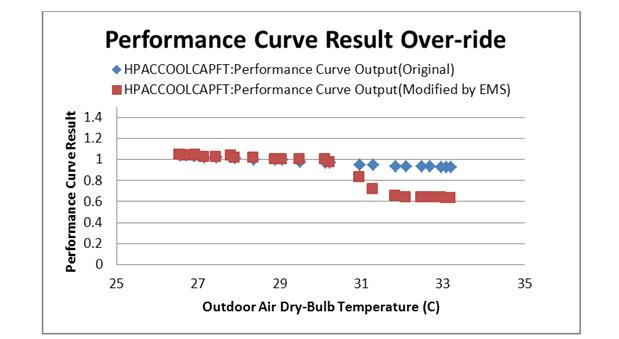
\includegraphics[width=0.9\textwidth, height=0.9\textheight, keepaspectratio=true]{media/image011.jpg}
\caption{Schematic for Exercise 1 \protect \label{fig:schematic-for-exercise-1}}
\end{figure}

The details of the building construction and operation are shown in the following tables and description. For tutorial purposes, the building is located in Chicago Illinois, one of the weather files supplied with EnergyPlus. These details are listed in a fashion to make for easy entry into EnergyPlus.

\subsection{Details of the exercise}\label{details-of-the-exercise}

\subsubsection{Surface Constructions}\label{surface-constructions}

{\scriptsize
\begin{longtable}[c]{>{\raggedright}p{0.85in}>{\raggedright}p{0.85in}>{\raggedright}p{0.85in}>{\raggedright}p{0.85in}>{\raggedright}p{0.85in}>{\raggedright}p{0.85in}>{\raggedright}p{0.85in}}
\toprule 
Material (listed from outside to inside) & Conductivity (W/m-K) & Thickness (m) & U (W/m-K) & R (m-K/W) & Density (kg/m) & C (J/kg-K) \tabularnewline
\midrule
\endfirsthead

\toprule 
Material (listed from outside to inside) & Conductivity (W/m-K) & Thickness (m) & U (W/m-K) & R (m-K/W) & Density (kg/m) & C (J/kg-K) \tabularnewline
\midrule
\endhead

Walls & ~ & ~ & ~ & ~ & ~ & ~ \tabularnewline
WOOD SIDING\--1 & 0.140 & 0.009 & 15.556 & 0.064 & 530 & 900 \tabularnewline
FIBERGLASS QUILT\--1 & 0.040 & 0.066 & 0.606 & 1.650 & 12 & 840 \tabularnewline
PLASTER\-BOARD\--1 & 0.160 & 0.012 & 13.333 & 0.075 & 950 & 840 \tabularnewline
Roof & ~ & ~ & ~ & ~ & ~ & ~ \tabularnewline
ROOF DECK & 0.140 & 0.019 & 7.368 & 0.136 & 530 & 900 \tabularnewline
FIBERGLASS QUILT-2 & 0.040 & 0.066 & 0.606 & 1.650 & 12 & 840 \tabularnewline
PLASTER\-BOARD-2 & 0.160 & 0.010 & 1.60 & 0.625 & 950 & 840 \tabularnewline
Floor & ~ & ~ & ~ & ~ & ~ & ~ \tabularnewline
C5 CONCRETE & 1.73 & 0.1015 & 17.04 & 0.059 & 2243 & 837 \tabularnewline
\bottomrule
\end{longtable}}

\subsubsection{Window Properties}\label{window-properties}

\begin{longtable}[c]{@{}ll@{}}
\toprule 
Type * & Clear \tabularnewline
\midrule
\endfirsthead

\toprule 
Type * & Clear \tabularnewline
\midrule
\endhead

Number of panes & 2 \tabularnewline
Pane thickness & 0.006 m \tabularnewline
Air-gap thickness & 0.0032 m \tabularnewline
Conductivity of glass & 0.9 W/m-K \tabularnewline
\bottomrule
\end{longtable}

Refers to specific glass type included in the EnergyPlus datasets directory

(\textbf{WindowGlassMaterials.idf})

\begin{longtable}[c]{>{\raggedright}p{1.5in}>{\raggedright}p{4.5in}}
\caption{Additional Model Details \label{table:additional-model-details}} \tabularnewline
\toprule 
Type & Details \tabularnewline
\midrule
\endfirsthead

\caption[]{Additional Model Details} \tabularnewline
\toprule 
Type & Details \tabularnewline
\midrule
\endhead

Internal Loads & Lights (1000 W), Office Lighting schedule, surface mount fluorescent \tabularnewline
Space Conditioning & Heating setpoint 20C, cooling setpoint 24C, no setback \tabularnewline
Location & Chicago, Illinois, USA; Summer and Winter design days \tabularnewline
Simulation Period & Annual, Jan 1 - Dec 31 \tabularnewline
Ground Temperatures & 18.2 C to 22.5 C (from Slab preprocessor, vary monthly) \tabularnewline
\bottomrule
\end{longtable}


\section{Instructions}\label{instructions-000}

\subsection{Exercise 1A. Run Pre-Defined Building with no Windows}\label{exercise-1a.-run-pre-defined-building-with-no-windows}

Objective:~ Learn to use EP-Launch to run an EnergyPlus input file and view output files.

1.~Open EP-Launch.

2.~Under ``Input File'', browse for input file Exercise1A.idf.~ This input file contains the 1-zone model described above without the windows and lights. This is located under the install folder \textless{}root\textgreater{}\textbackslash{}ExampleFiles\textbackslash{}BasicsFiles,

3.~Under ``Weather File'', select ``No Weather File'' (at the top of the pull-down list).

4.~Press ``Simulate''.

5.~When the simulation is complete, review output files:

\begin{itemize}
\item
  Press ``Text Output Files'' to see all text output.~ Look especially at the eio and err output files.
\item
  Press ``Drawing Files'' to see a dxf drawing of the building envelope.~ (If using Voloview Express, right-click to switch between wireframe and shaded orbit view.~ In DWG True View, use ``View'' -\textgreater{} ``Visual Styles'' to switch between wireframe and solid views. In both programs, use ``View'' à``Named Views'' to select isometric views.)
\item
  An empty svg drawing file will also open (this will show HVAC system components in later exercises).~ Note that the Adobe SVG viewer is a ``plug-in'' for Internet Explorer (IE), so IE will open when viewing an SVG file.~ Depending on the security settings in IE, you may be prompted with a warning about ``active'' content.
\item
  Press ``Spreadsheets'' to open the numeric csv output files.~ In Exercise1a.csv, review the pattern of outdoor conditions and loads.~ (To make it easier to read the column headings, select Row 1, format cells, and turn on wrap text; then select cell B2 and select ``freeze panes''.) ~In Exercise1aMeter.csv, review the facility district heating and cooling meters.
\item
  Zone/Sys Air Temperature -- the zone air temperatures are already being reported.
\item
  Outdoor Dry Bulb -- is being reported (so you can compare to outside temperature)
\item
  The meter for the heating in the facility - DistrictHeating:Facility -- is being reported. Facility is the entire building.
\item
  The meter for the cooling in the facility - DistrictCooling:Facility -- is being reported.
\end{itemize}

\subsection{Exercise 1B. Add Windows}\label{exercise-1b.-add-windows}

Objective:~ Learn how to add materials, constructions, and a surface using 3-D coordinates.

1.~In EP-Launch, with input file Exercise1A.idf still selected, press ``Edit -- IDF Editor''.~ This will open Exercise1A.idf in the IDF Editor, a tool that assists in editing EnergyPlus input files (idf).

2.~In IDF Editor, select File -\textgreater{} Save Options . . . and set ``Saved Order'' to ``Original with New at Top'', and ``Special Format for Some Objects'' to ``Yes.''~ Check the ``Set as Default'' box.

3.~In IDF Editor, Select File -\textgreater{} Save As . . . and save this file as Exercise1B.idf.

4.~Create the construction definition for the windows which are double-pane clear gas with an air space:

\begin{itemize}
\item
  Using File -\textgreater{} Open Dataset, open the window glass materials dataset file, WindowGlassMaterials.idf
\item
  Scroll down the Class list and select ``\textbf{WindowMaterial:Glazing}''.
\end{itemize}

\begin{lstlisting}
-Hint:  In IDF Editor, View -> Show Classes with Objects Only (or ctl-L) will hide all empty object types from the class list.
\end{lstlisting}

\begin{itemize}
\item
  Locate the object which defines the material properties for ``CLEAR 6MM''.~ Select this object (by clicking on the column heading).
\item
  Using Edit -\textgreater{} Copy Object (or the toolbar button, or ctl-C), copy this object.
\item
  Switch windows to file Exercise1B.idf and paste the window material into this file.~ (Verify that is had been added by going to \textbf{WindowMaterial:Glazing} to view the object.)
\item
  Open dataset file WindowGasMaterials.idf.
\item
  Locate ``AIR 3MM'', copy it and paste it into Exercise1B.idf.
\item
  In Exercise1B.idf, select the ``\textbf{Construction}'' class.~ There are three constructions pre-defined for the walls, roof, and floor.
\item
  Press ``New Obj'' to create a new blank \textbf{Construction} object.
\item
  Name this new construction ``DOUBLE PANE WINDOW''.
\item
  Use the pulldown list to select ``CLEAR 6MM'' for the outside layer, then press ``Enter'' or ``Return'' to save this entry and move to the next field.
\item
  Select ``AIR 3MM'' for Layer 2, and ``CLEAR 6MM'' for Layer 3.
\end{itemize}

5.~Add the east window (3m wide by 2m high, centered on wall, \emph{see the drawing in} \emph{Figure~\ref{fig:schematic-for-exercise-1}} \emph{to determine coordinates):}

\begin{itemize}
\item
  Select ``\textbf{FenestrationSurface:Detailed}'' class.
\item
  Add a new object named ``EAST WINDOW''.
\item
  Set the remaining fields as listed:
\item
  Surface Type \ldots{}\ldots{}\ldots{}\ldots{}\ldots{}\ldots{}\ldots{}\ldots{}\ldots{}\ldots{}\ldots{}\ldots{}\ldots{}\ldots{}\ldots{}\ldots{} = Window
\item
  Construction Name \ldots{}\ldots{}\ldots{}\ldots{} = DOUBLE PANE WINDOW
\item
  Base Surface Name \ldots{}\ldots{}\ldots{}\ldots{}\ldots{} = ZONE SURFACE EAST
\item
  OutsideFaceEnvironment Object \ldots{}\ldots{}\ldots{}\ldots{}\ldots{}\ldots{}. = \textless{}blank\textgreater{}
\item
  View Factor to Ground \ldots{}\ldots{}\ldots{}\ldots{}\ldots{}\ldots{}\ldots{}\ldots{}.. = autocalculate
\item
  Name of shading control \ldots{}\ldots{}\ldots{}\ldots{}\ldots{}\ldots{}\ldots{}\ldots{}\ldots{}\ldots{} = \textless{}blank\textgreater{}
\item
  WindowFrameAndDivider Name \ldots{}\ldots{}\ldots{}\ldots{}\ldots{}\ldots{}.. = \textless{}blank\textgreater{}
\item
  Multiplier \ldots{}\ldots{}\ldots{}\ldots{}\ldots{}\ldots{}\ldots{}\ldots{}\ldots{}\ldots{}\ldots{}\ldots{}\ldots{}\ldots{}\ldots{}\ldots{}\ldots{}\ldots{}\ldots{}\ldots{}\ldots{}. = 1
\item
  Number of Surface Vertex Groups \ldots{}\ldots{}\ldots{}\ldots{}\ldots{}\ldots{}\ldots{}\ldots{}\ldots{} = 4
\item
  Vertex coordinates = \emph{as determined from the drawing} \emph{Figure~\ref{fig:schematic-for-exercise-1}}.~ Coordinates in this input are in World Coordinates (all relative to the global origin of 0,0,0).~ Coordinates are specified as viewed from the outside of the surface, using the rules specified in the SurfaceGeometry object.
\end{itemize}

6.~Add the west window, similar to the east window.

7.~Add a new \textbf{Output:Surfaces:List} object, type = Details.~ This report produces a list of all surfaces in the eio output summarizing area, azimuth, tilt, etc.

8.~Save and close the IDF file, select Exercise1B.idf in EP-Launch, run the simulation and view outputs.

\begin{itemize}
\item
  Always review the err file for errors and warnings.~ Fix problems if needed and re-run.
\item
  Are the windows in the right place in the dxf drawing file. (Use the Drawing File button or select the DXF file from View -\textgreater{} Single File or from the Quick-Open panel).
\item
  Review the surface details report in the eio file, search for ``Zone/Shading Surfaces'' to find this report. (Use the Text Output button, Quick Open ``eio'' button, or select from the single file menu, or use F7).~ This report is easier to read by pasting this section into a spreadsheet and using the text to columns function with comma as a delimiter).
\item
  Open the csv output file and compare the heating and cooling loads with the results from Exercise1A.csv.
\end{itemize}

\subsection{Exercise 1C. Add Internal Loads}\label{exercise-1c.-add-internal-loads}

Objective:~ Learn how to add schedules, internal loads, and report variables.

1.~Save Exercise1B.idf as Exercise1C.idf.

2.~Open the dataset file Schedules.idf:

\begin{itemize}
\item
  Copy the \textbf{Schedule:Compact} object named ``Office Lighting'', and paste it into Exercise1C.idf.
\item
  Copy the \textbf{ScheduleTypeLimits} object named ``Fraction'', and paste it into Exercise1C.idf.
\end{itemize}

3.~In Exercise1C.idf, add a LIGHTS object named ZONE ONE Lights, using the Office Lighting schedule, peak input is 1000W.~ Consult the EnergyPlus Input Output Reference section on \textbf{Lights} for values for the return, radiant, and visible fractions.~ Assume the lights are surface mounted fluorescents.

4.~Save and close the IDF file, select Exercise1C.idf in EP-Launch, run the simulation and review outputs.

5.~Open the rdd file (the report variable data dictionary) and find report variable names related to \textbf{Lights}.~ Add a new \textbf{Output:Variable} object to report the lighting electric consumption.

6.~Run the simulation and review outputs.

\begin{itemize}
\item
  Check the err file.
\item
  Find the lighting electric consumption in the csv output file.
\end{itemize}

7.~Compare heating and cooling loads with Exercise1A and Exercise1B.

8.~Add more \textbf{Output:Variable} objects as desired.

\subsection{Exercise 1D. Annual Simulation and Predefined Reports}\label{exercise-1d.-annual-simulation-and-predefined-reports}

Objective:~ Learn how to run an annual simulation using a weather data file and add table reports.

1.~Save Exercise1C.idf as Exercise1D.idf.

2.~Edit the \textbf{SimulationControl} object to turn off the design day simulations by setting ``Run Simulation for Sizing Periods'' to \textbf{No} and turn on the weather file (annual) simulation by setting ``Run Simulation for Weather File Run Periods'' to \textbf{Yes}..

3.~Add a RunPeriod object to run a full annual simulation, let other fields default or remain blank.

4.~Add a \textbf{Output:Table:SummaryReports} object, and select the following reports:~ ``Annual Building Performance Summary'' (ABUPS), ``Input Verification and Results Summary'' (IVRS), ``Climate Summary'', and ``Envelope Summary''.

5.~Add a \textbf{OutputControl:Table:Style} object, and select HTML format (ColumnSeparator).

6.~Edit existing \textbf{Output:Variable} and \textbf{Output:Meter} objects and change the reporting frequency from Hourly to Monthly.

7.~Save and close the IDF file, select Exercise1D.idf in EP-Launch.

8.~Select Chicago TMY2 weather file (or the weather file of your choice) and run the simulation.

9.~Review outputs.

\begin{itemize}
\item
  Check the err file.
\item
  Look at the monthly results in the csv output.
\item
  Press the Table output button to view the predefined reports.
\end{itemize}

\subsection{Solution: Exercise 1}\label{solution-exercise-1}

\emph{Try not to look at this section until you have completed the Exercise.}

\subsubsection{List of New Objects}\label{list-of-new-objects}

This is a listing of new and modified objects created in this Exercise.

\begin{lstlisting}
WindowMaterial:Glazing,
    CLEAR 6MM,               !- Name
    SpectralAverage,         !- Optical Data Type
    ,                        !- Name of Window Glass Spectral Data Set
    0.006,                   !- Thickness {m}
    0.775,                   !- Solar Transmittance at Normal Incidence
    0.071,                   !- Solar Reflectance at Normal Incidence: Front Side
    0.071,                   !- Solar Reflectance at Normal Incidence: Back Side
    0.881,                   !- Visible Transmittance at Normal Incidence
    0.080,                   !- Visible Reflectance at Normal Incidence: Front Side
    0.080,                   !- Visible Reflectance at Normal Incidence: Back Side
    0.0,                     !- IR Transmittance at Normal Incidence
    0.84,                    !- IR Hemispherical Emissivity: Front Side
    0.84,                    !- IR Hemispherical Emissivity: Back Side
    0.9;                     !- Conductivity {W/m-K}
\end{lstlisting}

\begin{lstlisting}
WindowMaterial:Gas,
    AIR 3MM,                 !- Name
    Air    ,                 !- Gas Type
    0.0032;                  !- Thickness {m}
\end{lstlisting}

\begin{lstlisting}
Construction,
    DOUBLE PANE WINDOW,      !- Name
    CLEAR 6MM,               !- Outside Layer
    AIR 3MM,                 !- Layer #2
    CLEAR 6MM;               !- Layer #3
\end{lstlisting}

\begin{lstlisting}
FenestrationSurface:Detailed,
    EAST WINDOW,             !- User Supplied Surface Name
    WINDOW,                  !- Surface Type
    DOUBLE PANE WINDOW,      !- Construction Name of the Surface
    ZONE SURFACE EAST,       !- Base Surface Name
    ,                        !- OutsideFaceEnvironment Object
    autocalculate,           !- View Factor to Ground
    ,                        !- Name of shading control
    ,                        !- WindowFrameAndDivider Name
    1,                       !- Multiplier
    4,                       !- Number of vertices
    8, 1.5, 2.35,            !- X,Y,Z  1 {m}
    8, 1.5, 0.35,            !- X,Y,Z  2 {m}
    8, 4.5, 0.35,            !- X,Y,Z  3 {m}
    8, 4.5, 2.35;            !- X,Y,Z  4 {m}
\end{lstlisting}

\begin{lstlisting}
FenestrationSurface:Detailed,
    WEST WINDOW,             !- User Supplied Surface Name
    WINDOW,                  !- Surface Type
    DOUBLE PANE WINDOW,      !- Construction Name of the Surface
    ZONE SURFACE WEST,       !- Base Surface Name
    ,                        !- OutsideFaceEnvironment Object
    autocalculate,           !- View Factor to Ground
    ,                        !- Name of shading control
    ,                        !- WindowFrameAndDivider Name
    1,                       !- Multiplier
    4,                       !- Number of Vertices
    0, 4.5, 2.35,            !- X,Y,Z  1 {m}
    0, 4.5, 0.35,            !- X,Y,Z  2 {m}
    0, 1.5, 0.35,            !- X,Y,Z  3 {m}
    0, 1.5, 2.35;            !- X,Y,Z  4 {m}
\end{lstlisting}

\begin{lstlisting}
Output:Surfaces:List,Details;
\end{lstlisting}

\begin{lstlisting}
Schedule:Compact,
    Office Lighting,         !- Name
    Fraction,                !- ScheduleType
    Through: 12/31,          !- Complex Field #1
    For: Weekdays SummerDesignDay,  !- Complex Field #2
    Until: 05:00, 0.05,      !- Complex Field #4
    Until: 07:00, 0.1,       !- Complex Field #6
    Until: 08:00, 0.3,       !- Complex Field #8
    Until: 17:00, 0.9,       !- Complex Field #10
    Until: 18:00, 0.5,       !- Complex Field #12
    Until: 20:00, 0.3,       !- Complex Field #14
    Until: 22:00, 0.2,       !- Complex Field #16
    Until: 23:00, 0.1,       !- Complex Field #18
    Until: 24:00, 0.05,      !- Complex Field #20
    For: Saturday WinterDesignDay,  !- Complex Field #21
    Until: 06:00, 0.05,      !- Complex Field #23
    Until: 08:00, 0.1,       !- Complex Field #25
    Until: 12:00, 0.3,       !- Complex Field #27
    Until: 17:00, 0.15,      !- Complex Field #29
    Until: 24:00, 0.05,      !- Complex Field #31
    For: Sunday Holidays AllOtherDays,  !- Complex Field #32
    Until: 24:00, 0.05;      !- Complex Field #34
\end{lstlisting}

\begin{lstlisting}
ScheduleTypeLimits,
    Fraction,                !- ScheduleType Name
    0.0,                     !- Lower Limit Value
    1.0,                     !- Upper Limit Value
    CONTINUOUS;              !- Numeric Type
\end{lstlisting}

\begin{lstlisting}
Lights,
    ZONE ONE Lights,         !- Name
    ZONE ONE,                !- Zone Name
    Office Lighting,         !- Schedule Name
    LightingLevel,           !- Design Level Calculation Method
    1000,                    !- Lighting Level {W}
    ,                        !- Watts per Zone Floor Area {W/m2}
    ,                        !- Watts per Person {W/person}
    0,                       !- Return Air Fraction
    0.72,                    !- Fraction Radiant
    0.18,                    !- Fraction Visible
    1,                       !- Fraction Replaceable
    General,                 !- End-Use Subcategory
    No;                      !- Return Air Fraction Calculated from Plenum Temperature
\end{lstlisting}

\begin{lstlisting}
Output:Variable,*,Lights Electric Consumption ,hourly;
\end{lstlisting}

\begin{lstlisting}
RunPeriod,
    1,                       !- Begin Month
    1,                       !- Begin Day Of Month
    12,                      !- End Month
    31,                      !- End Day Of Month
    UseWeatherFile,          !- Day Of Week For Start Day
    Yes,                     !- Use WeatherFile Holidays/Special Days
    Yes,                     !- Use WeatherFile DaylightSavingPeriod
    No,                      !- Apply Weekend Holiday Rule
    Yes,                     !- Use WeatherFile Rain Indicators
    Yes,                     !- Use WeatherFile Snow Indicators
    1;                       !- Number of years of simulation
\end{lstlisting}

\begin{lstlisting}
Output:Table:SummaryReports,
    Annual Building Utility Performance Summary,  !- ReportName1
    Input Verification and Results Summary,  !- ReportName2
    Climate Summary,         !- ReportName3
    Envelope Summary;        !- ReportName4
\end{lstlisting}

\begin{lstlisting}
OutputControl:Table,
    HTML;                    !- ColumnSeparator
\end{lstlisting}

\begin{lstlisting}
SimulationControl,
    No,                      !- Do the zone sizing calculation
    No,                      !- Do the system sizing calculation
    No,                      !- Do the plant sizing calculation
    No,                      !- Do the design day simulations
    Yes;                     !- Do the weather file simulation
\end{lstlisting}


\chapter{Overall scheme/methodology for running EnergyPlus}\label{overall-schememethodology-for-running-energyplus}


\section{Building Simulation}\label{building-simulation}

If you are already familiar with modeling buildings, particularly modeling buildings for energy consumption, you may wish to skip to ``IDF Editor -- Brief Introduction''. The following steps are general guidelines for using any building simulation program.


\section{A Methodology for Using Energyplus}\label{a-methodology-for-using-energyplus}

This section provides a step by step outline that will help you streamline creating your building models for using EnergyPlus.

\subsection{\emph{Step 1}: Plan Ahead}\label{step-1-plan-ahead}

Some preliminary steps will facilitate the construction of your input file. EnergyPlus requires some information in specified, externally available formats; other information may require some lead time to obtain. The following checklist should be completed before you start to construct your input file.

\begin{itemize}
\item
  Obtain location and design climate information for the city in which your building is located. If possible, use one of the weather files available for your weather period run.
\item
  Obtain sufficient \emph{building} \emph{construction} information to allow specification of overall building geometry and surface constructions (including exterior walls, interior walls, partitions, floors, ceilings, roofs, windows and doors).
\item
  Obtain sufficient \emph{building} \emph{use} information to allow specification of the lighting and other equipment (e.g.~electric, gas, etc.) and the number of people in each area of the building.
\item
  Obtain sufficient \emph{building} \emph{thermostatic} \emph{control} information to allow specification of the temperature control strategy for each area of the building.
\item
  Obtain sufficient \emph{HVAC} \emph{operation} information to allow specification and scheduling of the fan systems.
\item
  Obtain sufficient \emph{central plant} information to allow specification and scheduling of the boilers, chillers and other plant equipment.
\end{itemize}

\subsection{*Step 2: ``*Zone" the Building}\label{step-2-zone-the-building}

A building ``surface'' is the fundamental element in the building model. In the general sense, there are two types of ``surfaces'' in EnergyPlus. These are:

1.~~ heat transfer surfaces~ and

2.~~ heat storage surfaces

The first rule of building modeling is, ``\emph{Always define a surface as a heat storage surface unless it must be defined as a heat transfer surface}''. Any surface, which is expected to separate spaces of significantly different temperatures, must be defined as a \emph{heat transfer surface.} Thus, exterior surfaces, such as outside walls, roofs and floors, are \emph{heat transfer surfaces}. Interior surfaces (partitions) are \emph{heat storage surfaces} if they separate spaces maintained at the same temperature and \emph{heat transfer surfaces} if they separate spaces maintained at different temperatures. A discussion of how to define heat transfer and heat storage surfaces will occur in later steps. In order to correctly ``zone'' the building it is necessary only to distinguish between the two.

A ``zone'' is a \emph{thermal,} not a \emph{geometric,} concept. A ``zone'' is an air volume at a uniform temperature plus all the heat transfer and heat storage surfaces bounding or inside of that air volume. EnergyPlus calculates the energy required to maintain each zone at a specified temperature for each hour of the day. Since EnergyPlus performs a zone heat balance, the first step in preparing a building description is to break the building into zones. The objective of this exercise is to define as \emph{few} zones as possible without significantly compromising the integrity of the simulation.

Although defining building zones is somewhat of an art, a few general rules will keep the new simulation user out of trouble. Consider the following figure, which shows the floor plan of an Adult Education Center.

\begin{figure}[hbtp] % fig 12
\centering
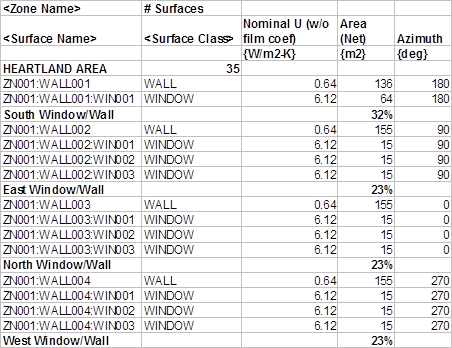
\includegraphics[width=0.9\textwidth, height=0.9\textheight, keepaspectratio=true]{media/image012.png}
\caption{Adult Education Center \protect \label{fig:adult-education-center}}
\end{figure}

The question is, ``How many \emph{thermal} zones should be used to model this building?''~ The inexperienced building modeler may be tempted to define each room in the building as a zone, but the thermal zone is defined as a volume of air at a uniform temperature. The general rule then is to \emph{use the number of fan systems (and radiant systems) not the number of rooms to determine the number of zones in the building.} The minimum number of zones in a general simulation model will usually be equal to the number of systems serving the building. The collection of heat transfer and heat storage surfaces defined within each zone will include all surfaces bounding or inside of the space conditioned by the system.

\subsection{Zoning -- Concept 1 - Simple}\label{zoning-concept-1---simple}

Complete estimates of the total building load (magnitude only) may be obtained with very simple models. For example the total building load calculated using a one-zone model of the Education Center (Figure~\ref{fig:single-zone-model-of-the-adult-education}) will \textbf{NOT} be significantly different from the total building load calculated using a more detailed model. The \emph{distribution} of the load within the building cannot be estimated with the simplified building model, but its \emph{magnitude} (such as would be used in sizing the central plant equipment) can be quickly estimated using a very simple model. For simplicity, assume there is no ground heat transfer; if you want to simulate ground heat transfer, you should use the slab and/or basement programs as described in the Auxiliary Programs document.

\begin{figure}[hbtp] % fig 13
\centering
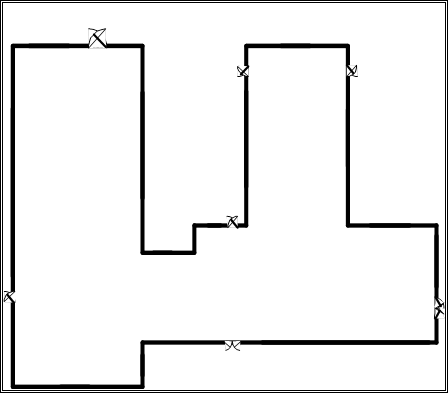
\includegraphics[width=0.9\textwidth, height=0.9\textheight, keepaspectratio=true]{media/image013.png}
\caption{Single Zone Model of the Adult Education Center. \protect \label{fig:single-zone-model-of-the-adult-education}}
\end{figure}

\subsection{Zoning -- Concept 2 - Detailed}\label{zoning-concept-2---detailed}

A more detailed model will allow you to determine more accurately the actual distribution of loads/energy within the building. In a more detailed model of the education center, five systems were designed to serve the Adult Education Center. These systems with the thermal zones they serve are shown in the table below. The location of each zone is shown in accompanying figure.

% table 2
\begin{longtable}[c]{@{}lllll@{}}
\caption{Zoning the Building by System Type. \label{table:zoning-the-building-by-system-type.}} \tabularnewline
\toprule 
System Number & System Name & CFM & m/s & Zone Served \tabularnewline
\midrule
\endfirsthead

\caption[]{Zoning the Building by System Type.} \tabularnewline
\toprule 
System Number & System Name & CFM & m/s & Zone Served \tabularnewline
\midrule
\endhead

1 & Four Pipe Fan Coil & 3900 & 19.812 & Zone 1 \tabularnewline
1 & Four Pipe Fan Coil & 2500 & 12.7 & Zone 2 \tabularnewline
2 & Single Zone Draw Through & 1400 & 7.112 & Zone 3 \tabularnewline
3 & Single Zone Draw Through & 2250 & 11.43 & Zone 5 \tabularnewline
4 & Single Zone Draw Through & 2450 & 12.446 & Zone 6 \tabularnewline
5 & Unit Heater & 185 & .9398 & Zone 4 \tabularnewline
5 & Unit Heater & 41 & .20828 & Zone 7 \tabularnewline
\bottomrule
\end{longtable}

\begin{figure}[hbtp] % fig 14
\centering
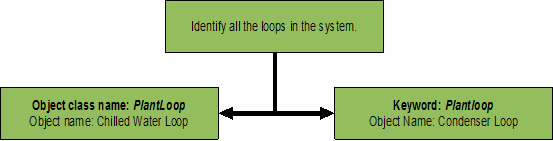
\includegraphics[width=0.9\textwidth, height=0.9\textheight, keepaspectratio=true]{media/image014.png}
\caption{Thermal Zones in the Education Center \protect \label{fig:thermal-zones-in-the-education-center}}
\end{figure}

Take note of Zone 1, Zone 2, Zone 4, and Zone 7. The two important zoning concepts can be demonstrated with the zoning to reinforce the idea of a thermal zone and encourage the use of simplified models.

1.~~ Notice that Zones 4 and 7 include two rooms that are not adjacent to one another but are served by the same system. Because the air temperature in the two spaces is maintained at the same uniform temperature, the two spaces, though separated spatially, may be defined as a single zone. For our purposes, we will define them as separate zones.

2.~~ Notice that Zone 1 and Zone 2 are served by the same fan system and could be defined as a single zone with 7650 cfm of conditioned air supplied to the space. The space was split into two zones because the designer expected higher solar loads on the South and West sides of the wing and wanted to examine the \emph{distribution} as well as the \emph{magnitude} of the load in the space.

\subsection{\emph{Step 3:} Prepare to Construct the Building Model}\label{step-3-prepare-to-construct-the-building-model}

Working from blueprints or sketches and following the guidelines in Step 2, the building zones were determined. It is recommended that the engineer sketch the building with its zones. Surface dimensions should be included in the sketch. Additional geometric and surface information is required before an input file describing the building can be constructed. Specifically the building model must:

1.~~ Determine \emph{heat transfer} and \emph{heat storage} surfaces.

2.~~ Define equivalent surfaces.

3.~~ Specify surfaces and subsurfaces (windows, doors, etc.) construction and materials.

4.~~ Compile surface and subsurface information.

By the way, the file for this example, the 1 zone model are contained in your EnergyPlus installation ExampleFiles\textbackslash{}BasicFiles folder.

\subsubsection{Step 3.1.~~~~~ Determine heat transfer and heat storage surfaces.}\label{step-3.1.-determine-heat-transfer-and-heat-storage-surfaces.}

The surfaces of the building can be described in any order; grouping surfaces by zone may help you read the input file. Specifics of the describing surfaces help categorize the surface's heat transfer/storage as well as identify the surface construction information.

The details of inputting surfaces are described in the Input/Output Reference document. The allowable surface types are shown in the following table:

% table 3
\begin{longtable}[c]{p{1.61in}p{4.38in}}
\caption{Surface types and categorization \label{table:surface-types-and-categorization}} \tabularnewline
\toprule 
Surface Type & Applicability \tabularnewline
\midrule
\endfirsthead

\caption[]{Surface types and categorization} \tabularnewline
\toprule 
Surface Type & Applicability \tabularnewline
\midrule
\endhead

BuildingSurface:Detailed & Wall, Roof, Ceiling, Floor \tabularnewline
FenestrationSurface:Detailed & Window, Door, Glassdoor \tabularnewline
InternalMass & Areas internal to a zone \tabularnewline
Shading:Site:Detailed & Shading devices external to the building face (other buildings, trees, etc.) \tabularnewline
Shading:Zone:Detailed & Shading devices attached to the building (overhang, fin) \tabularnewline
\bottomrule
\end{longtable}

The pieces of the definition that designate BuildingSurface:Detailed surfaces as either \emph{heat transfer} or \emph{heat storage} surfaces are:

\begin{lstlisting}

  A5 , \field Outside Boundary Condition
         \required-field
         \type choice
         \key Surface
         \key Zone
         \key Outdoors
         \key Ground
         \key OtherSideCoefficients
         \key OtherSideConditionsModel
    A6,  \field Outside Boundary Condition Object
         \type object-list
         \object-list OutFaceEnvNames
         \note Non-blank only if the field Outside Boundary Condition is Surface, Zone, OtherSideCoefficients,
         \note or OtherSideConditionsModel
         \note If Surface, specify name of corresponding surface in adjacent zone or
         \note specify current surface name for internal partition separating like zones
         \note If Zone, specify the name of the corresponding zone and
         \note the program will generate the corresponding interzone surface
         \note If OtherSideCoefficients, specify name of SurfaceProperty:OtherSideCoefficients
         \note If OtherSideConditionsModel, specify name of SurfaceProperty:OtherSideConditionsModel
    A7 , \field Sun Exposure
         \required-field
         \type choice
         \key SunExposed
         \key NoSun
         \default SunExposed
    A8,  \field Wind Exposure
         \required-field
         \type choice
         \key WindExposed
         \key NoWind
         \default WindExposed
\end{lstlisting}

Note that subsurfaces (windows, doors) on these base surfaces will inherit the base surface properties listed above. The following examples will use a bit more of the Surface definition to give context.

Surfaces that specify ``themselves'' as the outside boundary condition are ceilings, floors and partitions that divide temperature-controlled spaces. The program assumes that the surface temperatures on both sides of the surface are the same. This means that even though heat may be stored in a partition, ceiling, or floor, no heat flows \emph{through} it.

Heat Storage Surfaces (Use current Surface name for ExteriorEnvironment), e.g.:

\begin{lstlisting}

BuildingSurface:Detailed,Zn005:Wall006,  !- Base Surface Name
    Wall,INTERIOR,  !- Class and Construction Name
    MAINE WING,  !- Zone
    Surface, Zn005:Wall006,  !- Exterior Conditions and Target
     NoSun,  !- Solar Exposure
     NoWind,  !- Wind Exposure
    0.5000000    ,  !- VF to Ground
             4, !-Rectangle
     57.90000    ,   57.79000    ,   10.00000    ,
     57.90000    ,   57.79000    ,  0.0000000E+00,
     57.90000    ,   47.79000    ,  0.0000000E+00,
     57.90000    ,   47.79000    ,   10.00000    ;
\end{lstlisting}

Some surfaces divide the temperature controlled space from the outside environment. Surfaces that are both sun and wind exposed (e.g.~exterior walls, exposed floors, roofs) feel the full effect of both solar radiation and outside temperature, and the outside air film resistance for these surfaces changes with wind speed and wind direction. Surfaces that are not sun or wind exposed (a wall to an ``uncontrolled'' space) are not affected by solar radiation, wind speed or direction and have a constant outside convective air film resistance.

Heat Transfer Surfaces Exposed to the Outside Environment, such as Exterior Walls, Roofs, Exposed Floors:

\begin{lstlisting}

BuildingSurface:Detailed,Zn005:Wall002,  !- Base Surface Name
    Wall,EXTERIOR,  !- Class and Construction Name
    MAINE WING,  !- Zone
    Outdoors,,  !- Exterior Conditions and Target (if applicable)
     SunExposed,  !- Solar Exposure
     WindExposed,  !- Wind Exposure
    0.5000000    ,  !- VF to Ground
             4, !-Rectangle
     77.90000    ,   47.79000    ,   10.00000    ,
     77.90000    ,   47.79000    ,  0.0000000E+00,
     77.90000    ,   67.79000    ,  0.0000000E+00,
     77.90000    ,   67.79000    ,   10.00000    ;
\end{lstlisting}

Surfaces such as basement walls and slab floors separate the space from the earth surrounding the surfaces. Therefore, the outside surface temperatures become the ground temperatures.

Heat Transfer Surfaces in Contact with the Ground, such as Basement Walls or Slab Floors:

\begin{lstlisting}

BuildingSurface:Detailed,Zn004:Flr001,  !- Base Surface Name
    Floor,SLAB FLOOR,  !- Class and Construction Name
    ARIZONA WING,  !- Zone
    Ground,,  !- Exterior Conditions and Target (if applicable)
     NoSun,  !- Solar Exposure
     NoWind,  !- Wind Exposure
     1.000000    ,  !- VF to Ground
             4, !-Rectangle
     38.01000    ,   8.510000    ,  0.0000000E+00,
     18.01000    ,   8.510000    ,  0.0000000E+00,
     18.01000    ,   28.51000    ,  0.0000000E+00,
     38.01000    ,   28.51000    ,  0.0000000E+00;
\end{lstlisting}

Other surfaces separate zones that may be at different temperatures. These surface types allow heat transfer (by conduction through the walls) from a zone at a higher temperature to a zone at a lower temperature. The location of the heat storage surface in the zone is not important except in specialized solar studies. The surface above (wall to uncontrolled space) would be more correctly modeled as an interzone surface.

Heat Transfer Surfaces Exposed to Another Zone, such as Interzone walls, ceilings or floors:

\begin{lstlisting}

BuildingSurface:Detailed,Zn005:Wall005,  !- Base Surface Name
    Wall,INTERIOR,  !- Class and Construction Name
    MAINE WING,  !- Zone
    Surface,Zn001:Wall009,  !- Exterior Conditions and Target
     NoSun,  !- Solar Exposure
     NoWind,  !- Wind Exposure
    0.5000000    ,  !- VF to Ground
             4, !-Rectangle
     57.90000    ,   47.79000    ,   10.00000    ,
     57.90000    ,   47.79000    ,  0.0000000E+00,
     67.90000    ,   47.79000    ,  0.0000000E+00,
     67.90000    ,   47.79000    ,   10.00000    ;
   
\end{lstlisting}

\subsubsection{Step 3.2.~~~~ Define equivalent surfaces as desired.}\label{step-3.2.-define-equivalent-surfaces-as-desired.}

When the building was zoned, our objective was to define as \emph{few} zones as possible. Now we would like to extend this objective to include defining as \emph{few} surfaces as possible without significantly compromising the integrity of the simulation. We reduce the number and complexity of surfaces in our input file by defining \emph{equivalent} surfaces.

Before dealing with equivalent surfaces, it is appropriate to take the concept of a thermal zone one step further. EnergyPlus performs heat balances on individual zone surfaces and on the zone air. For purposes of the heat transfer calculations, a \emph{geometrically} correct rendering of the zone surfaces is not required. The surfaces do not even have to be connected. As long as the program knows to which thermal zone (mass of air) each surface transfers heat, it will calculate all heat balances correctly. For example, all heat storage surfaces of the same construction within a zone may be defined as a single rectangular surface. The size of this \emph{equivalent} surface will equal the sum of all the areas of all the heat storage surfaces in the zone. A few simple rules will further explain what we mean by \emph{equivalent} surfaces and how these surfaces may be used. Remember that these are guidelines for optional simplification of input. Each simplification must be evaluated to determine if it would significantly impact certain shading, interior solar gains, or daylighting features. The goal is to seek an adequate level of detail to capture the key features of the building envelope without spending excess time describing and computing results for details that are insignificant.

1.~~ \emph{Define all roofs and floors as rectangles regardless of the shape of the zone.} Each zone may have one rectangular roof and one rectangular floor of a given construction.

2.~~ \emph{Define all heat storage surfaces of the same construction within a zone as a single surface}. The size of the single surface is obtained by summing the individual surface areas exposed to the zone. Thus, if a partition is completely within a zone (both sides of the partition are exposed to the zone), the area of each side must be added to the area of the equivalent surface. On the other hand, if the partition separates two zones, the area of only one side should be added to the equivalent surface.

3.~~ \emph{Combine all windows on a given exterior surface into a single window}. Usually each exterior surface should have only one window of each type. Overhangs or other shading devices may require that more windows be specified or combined together. By using the WindowMaterial:Glazing construction for your glass door, they will be correctly modeled in EnergyPlus with sunlight transferring into the zone.

The following figure shows the surfaces and subsurfaces required for a one-zone model, i.e., the education center. Since there were two types of partitions in the building, two heat storage surfaces (``internal mass'') of different constructions were defined.

\begin{figure}[hbtp] % fig 15
\centering
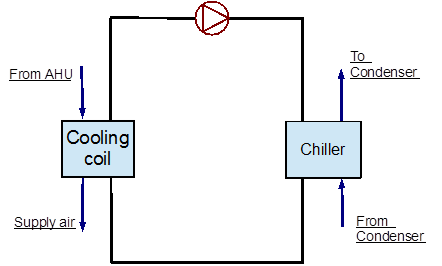
\includegraphics[width=0.9\textwidth, height=0.9\textheight, keepaspectratio=true]{media/image015.png}
\caption{Simplifications Using Equivalent Surfaces \protect \label{fig:simplifications-using-equivalent-surfaces}}
\end{figure}

\subsubsection{Step 3.3. Specify construction elements}\label{step-3.3.-specify-construction-elements}

BLAST, DOE-2 and other programs often have ``libraries'' of constructions, schedules, and other aspects of simulating the building. In EnergyPlus, we have a special set of files in the DataSets folder that represent many facets of building simulation. Data sets are usually IDF snippets or macro files. For constructions, using the guidelines in the ASHRAE Handbook of Fundamentals (2005), the file ASHRAE\_2005\_HOF\_Materials.idf contains materials and constructions from Chapters 30 and 25. Since Chapter 30 discusses heating and cooling loads, it includes constructions for light, medium and heavy weight buildings -- these constructions are represented in the dataset file. For the education center, ``medium'' constructions are used. For the windows, we will use the Double Pane Window from the previous exercise.

% table 4
\begin{longtable}[c]{@{}lll@{}}
\caption{Building Elements \label{table:building-elements}} \tabularnewline
\toprule 
Type (1) & Name (2) & Material (3) \tabularnewline
\midrule
\endfirsthead

\caption[]{Building Elements} \tabularnewline
\toprule 
Type (1) & Name (2) & Material (3) \tabularnewline
\midrule
\endhead

Wall & Medium Exterior Wall & M01 100mm brick \tabularnewline
~ & ~ & I02 50mm insulation board \tabularnewline
~ & ~ & F04 Wall air space resistance \tabularnewline
~ & ~ & G01a 19mm gypsum board \tabularnewline
Window & Double Pane Window & Clear 6MM \tabularnewline
~ & ~ & Air 3MM \tabularnewline
~ & ~ & Clear 6MM \tabularnewline
Partition & Medium/Heavy Partitions & G01a 19mm gypsum board \tabularnewline
~ & ~ & M01 100mm brick \tabularnewline
~ & ~ & M05 200mm concrete block \tabularnewline
~ & ~ & G01a 19mm gypsum board \tabularnewline
Partition & Medium Partitions & G01a 19mm gypsum board \tabularnewline
~ & ~ & F04 Wall air space resistance \tabularnewline
~ & ~ & G01a 19mm gypsum board \tabularnewline
Wall & Heavy/Medium Partitions & G01a 19mm gypsum board \tabularnewline
~ & ~ & M05 200mm concrete block \tabularnewline
~ & ~ & M01 100mm brick \tabularnewline
~ & ~ & G01a 19mm gypsum board \tabularnewline
Roof & Medium Roof/Ceiling & M14a 100mm heavyweight concrete \tabularnewline
~ & ~ & F05 Ceiling air space resistance \tabularnewline
~ & ~ & F16 Acoustic tile \tabularnewline
Floor & Medium Floor & F16 Acoustic tile \tabularnewline
~ & ~ & F05 Ceiling air space resistance \tabularnewline
~ & ~ & M14a 100mm heavyweight concrete \tabularnewline
\bottomrule
\end{longtable}

Notes:

(1)~ The surface type is a wall, floor, roof, window or door.

\begin{enumerate}
\def\labelenumi{(\arabic{enumi})}
\setcounter{enumi}{1}
\item
  User supplies name for the element. For this example use name from the DataSet: \textbf{ASHRAE\_2005\_HOF\_Materials.idf}. Similarly, the window was constructed from the \textbf{Windows.idf} dataset.
\item
  Material's full name is as found in the ASHRAE\_2005\_HOF\_Materials.idf dataset.
\end{enumerate}

\subsubsection{Step 3.4.~~~~ Compile surface and subsurface information.}\label{step-3.4.-compile-surface-and-subsurface-information.}

\emph{Building information:}

\emph{Building North Axis:} This syntax simplifies building geometry specification by designating one wall of the building as the building's north pointing axis. The building model North axis is measured from true (compass) North. Surface facing angles (see surface information below) are then specified relative to the building north axis. The \emph{North Axis} entry in the Input Output Reference (duplicated here) illustrates specification of the building north axis.

\begin{figure}[hbtp] % fig 16
\centering
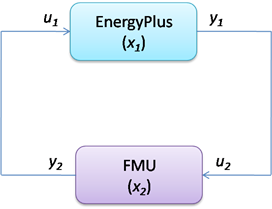
\includegraphics[width=0.9\textwidth, height=0.9\textheight, keepaspectratio=true]{media/image016.png}
\caption{Illustration of Building North Axis \protect \label{fig:illustration-of-building-north-axis}}
\end{figure}

\emph{Zone information:}

\begin{enumerate}
\def\labelenumi{\arabic{enumi}.}
\tightlist
\item
  \emph{Wall height}: In a simple model, one should make all the walls the same height. Then, the simple, 1 zone model can entirely enclose the space. In more complex models, you may resize each wall accordingly.
\end{enumerate}

\emph{Surface information:}

1.~~ \emph{Base} \emph{Surface Type:} Heat Transfer/Heat Storage Surfaces may be of the following types: wall, floor, roof, internal mass, or subsurface

2.~~ \emph{Construction:} The type of construction of the surface (see previous table).

\emph{Subsurface information:}

1.~~~~\emph{Subsurfaces} are Windows, Doors or GlassDoors

2.~~ \emph{Area:} Area of the subsurface.

3.~~ \emph{Reveal:} For windows only, the distance it is inset from the outside surface of a wall. For simplicity, put all the windows in the same physical plane as the wall they are on.

For the single zone model, the following figure is a schematic representation of a one zone representation. The figure shows the length of all ``base'' surfaces and the areas of all ``subsurfaces'' (windows). Doors are shown and may be entered, if desired. In the table (Table~\ref{table:compilation-of-surface-information-for}), the surfaces are numbered counter-clockwise around the zone beginning at the lower left corner of the figure. ~This table is the minimum required zone information compiled by the user. A few simple conventions should be followed to facilitate the construction of zone information tables:

1.~~ Number all surfaces in order counter-clockwise around the zone.

2.~~ Keep the subsurfaces with the base surface on which they are located.

3.~~ Specify \emph{lengths} for base surfaces and areas for subsurfaces and internal mass.

4.~~~~Specify the roof and floor as rectangles of the correct size.

\begin{figure}[hbtp] % fig 17
\centering
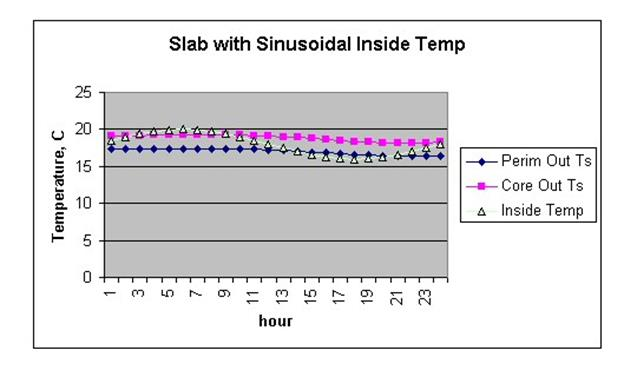
\includegraphics[width=0.9\textwidth, height=0.9\textheight, keepaspectratio=true]{media/image017.jpg}
\caption{Schematic of One Zone Model with Exterior Wall length and Window Areas. \protect \label{fig:schematic-of-one-zone-model-with-exterior}}
\end{figure}

\textbf{Full Building -- 1 Zone model}

% table 5
\begin{longtable}[c]{p{1.2in}p{1.2in}p{1.2in}p{1.2in}p{1.2in}}
\caption{Compilation of Surface Information for the One Zone Model \label{table:compilation-of-surface-information-for}} \tabularnewline
\toprule 
Surface & type & construction & Length \{m\} & Area \{m  \} \tabularnewline
\midrule
\endfirsthead

\caption[]{Compilation of Surface Information for the One Zone Model} \tabularnewline
\toprule 
Surface & type & construction & Length \{m\} & Area \{m  \} \tabularnewline
\midrule
\endhead

1 & exterior wall & Medium Exterior Wall & 15.25 & ~ \tabularnewline
2 & window & Double Pane Window & ~ & 5.62 \tabularnewline
3 & exterior wall & Medium Exterior Wall & 4.9 & ~ \tabularnewline
4 & window & Double Pane Window & ~ & 3.9 \tabularnewline
5 & exterior wall & Medium Exterior Wall & 34.44 & ~ \tabularnewline
6 & window & Double Pane Window & ~ & 33.7 \tabularnewline
7 & exterior wall & Medium Exterior Wall & 13.2 & ~ \tabularnewline
8 & window & Double Pane Window & ~ & 9.44 \tabularnewline
9 & exterior wall & Medium Exterior Wall & 10.4 & ~ \tabularnewline
10 & window & Double Pane Window & ~ & 7.58 \tabularnewline
11 & exterior wall & Medium Exterior Wall & 20 & ~ \tabularnewline
12 & window & Double Pane Window & ~ & 10.5 \tabularnewline
13 & exterior wall & Medium Exterior Wall & 12 & ~ \tabularnewline
14 & window & Double Pane Window & ~ & 7.58 \tabularnewline
15 & exterior wall & Medium Exterior Wall & 20 & ~ \tabularnewline
16 & window & Double Pane Window & ~ & 17.66 \tabularnewline
17 & exterior wall & Medium Exterior Wall & 6.1 & ~ \tabularnewline
18 & window & Double Pane Window & ~ & 4.7 \tabularnewline
19 & exterior wall & Medium Exterior Wall & 3.1 & ~ \tabularnewline
20 & exterior wall & Medium Exterior Wall & 6.1 & ~ \tabularnewline
21 & window & Double Pane Window & ~ & 3.71 \tabularnewline
22 & exterior wall & Medium Exterior Wall & 23 & ~ \tabularnewline
23 & window & Double Pane Window & ~ & 19.39 \tabularnewline
24 & exterior wall & Medium Exterior Wall & 15.24 & ~ \tabularnewline
25 & window & Double Pane Window & ~ & 7.8 \tabularnewline
26 & exterior wall & Medium Exterior Wall & 38 & ~ \tabularnewline
27 & window & Double Pane Window & ~ & 31 \tabularnewline
28 & roof & Medium Roof/Ceiling & Equivalent area (square) & 1250.1 \tabularnewline
29 & floor & Medium Floor & Equivalent area (square) & 1250.1 \tabularnewline
30 & internal mass & Medium Partitions & ~ & 956.9 \tabularnewline
31 & internal mass & Medium/Heavy Partitions & ~ & 1757.7 \tabularnewline
\bottomrule
\end{longtable}

The column headings in the previous table have the following meanings:

\textbf{Type:}~ A shortened notation for the surface type in EnergyPlus to differentiate between heat storage surfaces and various types of heat transfer surfaces.

\textbf{Construction:}~ A name for the surface construction types.

\textbf{Length:}~ The length of base surfaces (i.e.~Exterior Walls).

\textbf{Area:}~ The area of subsurfaces (windows), roofs, floors.

\subsection{Step 4: Compile Internal Space Gain Data}\label{step-4-compile-internal-space-gain-data}

People, lights, equipment, outside air infiltration and ventilation all constitute ``internal gains'' for the thermal zone. These gains are described to EnergyPlus as a \emph{design or} \emph{peak} level with a \emph{schedule} that specifies a fraction of the peak for each hour. The peak level is calculated by the user. Table~\ref{table:internal-gain-data}. Internal Gain Data shows the internal loads for a single zone model of Ft. Monmouth and the schedule named to specify the hourly load.

% table 6
\begin{longtable}[c]{@{}llll@{}}
\caption{Internal Gain Data \label{table:internal-gain-data}} \tabularnewline
\toprule 
Zone & Gain Type & Size & Schedule \tabularnewline
\midrule
\endfirsthead

\caption[]{Internal Gain Data} \tabularnewline
\toprule 
Zone & Gain Type & Size & Schedule \tabularnewline
\midrule
\endhead

1 & People & 205 & Office occupancy \tabularnewline
~ & Lights & 26360 W & Office lighting \tabularnewline
~ & ZoneInfiltration & .75 m  /sec & Constant \tabularnewline
\bottomrule
\end{longtable}

The column headings in the table have the following meanings:

\textbf{Gain Type:}~ The code used to differentiate between various types of internal gains.

\textbf{Size:}~ The peak load. This is the actual size of the load for every hour that the schedule specifies ``100\%''.

\textbf{Schedule:}~ The hourly schedule that specifies the percentage of peak load for each hour of the day.

\textbf{HVAC:} Using the Compact HVAC models, purchased air can be used to calculate the energy needs of the building.

As the following figure shows, the equivalent area floor/roof does not fit in the building perimeter. As an exercise, you might reconfigure both floor and roof to be a polygonal shape and compare results.

\begin{figure}[hbtp] % fig 18
\centering
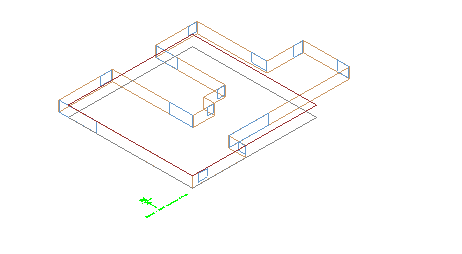
\includegraphics[width=0.9\textwidth, height=0.9\textheight, keepaspectratio=true]{media/image018.png}
\caption{Full Building - Adult Education Center \protect \label{fig:full-building-adult-education-center}}
\end{figure}

As an adjunct to the previous schematic layout for the one zone approach, the following figure shows the same building but with IP units:

\begin{figure}[hbtp] % fig 19
\centering
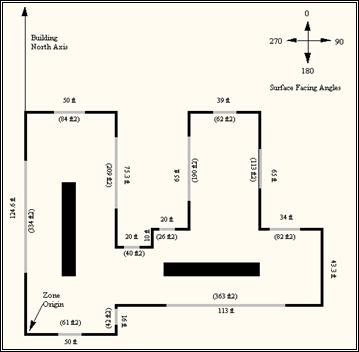
\includegraphics[width=0.9\textwidth, height=0.9\textheight, keepaspectratio=true]{media/image019.jpg}
\caption{Schematic for One Zone Building - IP Units \protect \label{fig:schematic-for-one-zone-building-ip-units}}
\end{figure}


\chapter{Tutorial Exercise 2}\label{tutorial-exercise-2}

The following example is taken directly from the training course ``Introduction to EnergyPlus'', Exercise 2.~ Of course, it is presented here without the benefit of classroom presentation and discussion but when followed step by step, should provide an introduction of actually using EnergyPlus.


\section{Unitary System and VAV using HVACTemplate Inputs}\label{unitary-system-and-vav-using-hvactemplate-inputs}

\subsection{Overview}\label{overview-000}

\begin{itemize}
\item
  Rectangular single story building with 5 occupied zones and a ceiling plenum
\item
  Packaged DX cooling with gas heat serving one zone
\item
  VAV with reheat and return plenum serving the other 4 zones
\item
  All equipment autosized using summer and winter design days
\end{itemize}

\begin{figure}[hbtp] % fig 20
\centering
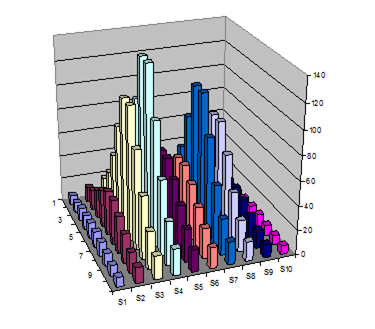
\includegraphics[width=0.9\textwidth, height=0.9\textheight, keepaspectratio=true]{media/image020.png}
\caption{Schematic for Exercise 2. \protect \label{fig:schematic-for-exercise-2.}}
\end{figure}

\subsection{Details of the Exercise}\label{details-of-the-exercise-000}

\subsubsection{Building Description}\label{building-description}

\begin{itemize}
\item
  Single floor rectangular building 30.5 m (100 ft) by 15.2 m (50 ft) by 3m (10 ft) high.
\item
  Building is oriented with the long axis running east-west.
\item
  Floor Area 463.6 m2 (5000 ft2).
\item
  5 occupied zones - 4 exterior, 1 interior, zone height 2.4 m (8 ft). Exterior zone depth is 3.7 m (12 ft).
\item
  1 plenum zone 0.6 m (2 ft) high.
\item
  Windows on all 4 facades
\item
  South and north facades have glass doors.
\item
  South facing glass is shaded by overhangs.
\item
  Walls are wood shingle over plywood, insulation, and gypsum board.
\item
  Roof is gravel built up roof with mineral board insulation and plywood sheathing.
\item
  Floor slab is 0.1 m (4 in) heavy concrete.
\item
  Windows and glass doors are double pane Low-e clear glass with argon gap.
\item
  Window to wall ratio is approximately 0.3.
\item
  Lighting is 16 W/m2 (1.5 W/ft2).
\item
  Office electric equipment is 10.8 W/m2 (1.0 W/ft2).
\item
  1 occupant per 9.3 m2 (100 ft2) of floor area.
\item
  Infiltration is 0.25 air changes per hour (always on, proportional to wind speed).
\item
  * Refers to specific glass type included in the EnergyPlus datasets directory
\item
  ~~~~~~~~~~~ (WindowGlassMaterials.idf)
\end{itemize}

\subsubsection{Space Conditioning}\label{space-conditioning}

\begin{itemize}
\item
  Heating setpoints:~~ 21.1C (70F) occupied, 12.8C (55F) unoccupied
\item
  Cooling setpoints:~~ 23.9C (75F) occupied, 40.0C (104F, system off) unoccupied
\item
  Plenum zone not controlled
\end{itemize}

\subsubsection{Environment}\label{environment}

\begin{itemize}
\item
  Location:~~~~~~~~~~~~~~~~~~ Chicago, Illinois, USA
\item
  Design Days:~~~~~~~~~~~~ Summer, Winter
\item
  Annual Simulation Period:~~~ Jan 1 -- Dec 31
\item
  Ground Temperatures:~~~~~~~~ from Slab preprocessor (20.4 to 23.0 C)
\end{itemize}


\section{Instructions}\label{instructions}

\subsection{Exercise 2A. Add Unitary System with DX Cooling and Gas Heating (Furnace) Serving a Single Zone}\label{exercise-2a.-add-unitary-system-with-dx-cooling-and-gas-heating-furnace-serving-a-single-zone}

Objective:~ Learn how to describe a thermostat and unitary equipment using HVACTemplate objects.

1)~~~Open Exercise2.idf and save it as Exercise2A.idf.~ (Exercise2.idf contains the building envelope, internal loads, and some extra schedules to support the HVAC system descriptions which will be added in this Exercise.)

2)~~~Add a \textbf{HVACTemplate:Thermostat} object to define the thermostat setpoints for this simulation.

\begin{itemize}
\item
  Choose a name for the thermostat.~ This name will be referenced in the next step.
\item
  For heating setpoints, use pre-defined schedule named ``Office Heating Setpoints''.
\item
  For cooling setpoints, use pre-defined schedule named ``Office Cooling Setpoints''.
\end{itemize}

3)~~~Add a \textbf{HVACTemplate:Zone:Unitary} object serving the ``NORTH PERIMETER'' zone.~ Choose a name for the air handling system which will be added in Step 4. Use the thermostat name from step 2 for the thermostat field. Retain the defaults for the remaining fields.

4)~~~Add a \textbf{HVACTemplate:System:Unitary} object.~ The name of this system object must be the same name used in the zone object for ``Air Handling System Name'' field (See Step 3).~ Retain the defaults for all fields except the following:

\begin{itemize}
\item
  Availability Schedule = Office HVAC (predefined)
\item
  Control Zone Name or Thermostat Location = NORTH PERIMETER
\item
  Supply Fan Operating Mode Schedule Name = Continuous
\item
  Heating Coil Type = Gas
\item
  Minimum Outdoor Air Schedule Name = Office Minimum OA (predefined)
\end{itemize}

5)~~~Add a \textbf{Sizing:Parameters} object and set the sizing factor to 1.2 (for 20\% oversizing).

6)~~~Edit the \textbf{SimulationControl} object and set the Zone and System sizing flags to ``Yes''.

7)~~~Run the simulation and review output files, especially:

\begin{itemize}
\item
  err, there will be some warnings about meters that do no exist and the ABUPS report not being a full year.~ These will go away as more features are added and an annual run is simulated.
\item
  DXF , drawing of building surfaces.~ (Try selecting the Southwest Isometric named view, then see how each zone is a separate drawing layer.~ In Voloview open the View -\textgreater{} Layers dialog.~ Click on the light bulbs to toggle display of each zone.~ In TrueView click on the Layer Properties Manager toolbar button.~ To toggle display of a layer, single-click a layer light bulb, then click apply.)
\item
  SVG, block diagram of the HVAC system components. (HINT: right-click in the drawing and read the Help to learn how to navigate in the SVG viewer.)
\item
  Main Results File (csv) and Meter File (Meter.csv).
\item
  eio, zone and system sizing results
\item
  Add output variables to report operation of the system (furnace) fan, heating coil, and cooling coil.~ Reference the RDD output file for variable names.
\end{itemize}

8)~~~Re-run the simulation and review results again.

\begin{itemize}
\tightlist
\item
  Note during hour 7 of the summer design day that ``NORTH PERIMETER:Zone/Sys Sensible Heating Rate\href{Hourly}{W}'' is nonzero, but the heating coil is off and the DX cooling coil shows a load.~ Why?~ This report variable reports the impact of the system on the zone (not the zone's demand for heating or cooling), averaged over the hour.~ The system fan is scheduled on at 6 a.m., but the outside air dampers are closed.~ The zone is not warm enough from the night to require cooling, so the circulating fan heat warms the zone slightly for a portion of the hour until the zone temperature exceeds the cooling setpoint and the DX coil comes on for the remainder of the hour.~ If the economizer were active, this would not occur.
\end{itemize}

\subsection{Exercise 2B. Add VAV System with Reheat Serving Four Zones with Chiller and Boiler Plant}\label{exercise-2b.-add-vav-system-with-reheat-serving-four-zones-with-chiller-and-boiler-plant}

Objective:~ Learn how to describe a VAV system with central plant using HVACTemplate objects.

1)~~~Save Exercise2A.idf as Exercise2B.idf.

2)~~~Add a \textbf{HVACTemplate:System:VAV} object.~ Retain the defaults for all fields except the following:

\begin{itemize}
\item
  Air Handling System Name = \textless{}assign a name\textgreater{}
\item
  System Availability Schedule = Office HVAC (predefined)
\item
  Cooling Coil Design Setpoint = 13C (55.4F)
\item
  Minimum Outdoor Air Schedule Name = Office Minimum OA (predefined)
\item
  Economizer Type = FixedDryBulb
\item
  Return Plenum Name = PLENUM
\end{itemize}

3)~~~Add four \textbf{HVACTemplate:Zone:VAV} objects serving the four remaining zones (South Perimeter, East Perimeter, West Perimeter, and Core).~ Retain the defaults for all fields except the following:

\begin{itemize}
\item
  Specify the same air handler name added in Step 2 (use the dropdown list)
\item
  Specify the same thermostat control added in Exercise 2A Step 2 (again, use the dropdown list).
\item
  Supply Air Minimum Flow Fraction = 0.2
\item
  Reheat Coil Type = Hot Water
\item
  Heating Damper Action = Reverse
\item
  HINT:~ Define one \textbf{HVACTemplate:Zone:VAV} object, make the above changes to defaults, then press ``Dup Obj'' three times to duplicate the object, then edit the remaining three zone names.
\end{itemize}

4)~~~Add a \textbf{HVACTemplate:Plant:ChilledWaterLoop} object and assign a name.~~~ Retain the defaults for all fields except the following:

\begin{itemize}
\tightlist
\item
  Condenser Water Temperature Control Type = Specified Setpoint
\end{itemize}

5)~~~Add a \textbf{HVACTemplate:Plant:Chiller} object, type Electric Reciprocating Chiller with a nominal COP of 3.6, water cooled.

6)~~~Add a \textbf{HVACTemplate:Plant:Tower} object, type Two Speed.

7)~~~Add a \textbf{HVACTemplate:Plant:HotWaterLoop} object and assign a name.~ Retain the defaults for all fields.

8)~~~Add a natural gas fired hot water boiler using \textbf{HVACTemplate:Plant:Boiler}.

9)~~~Run the simulation, add desired report variables, and re-run the simulation.~ Review results and compare with results from Exercise 2A:

\begin{itemize}
\item
  Note how the heating and cooling rates for the NORTH PERIMETER zone are smaller than before.~ Why?
\item
  Review the SVG drawing to see the components of the VAV system and water loops.
\item
  Browse the expidf file in a text editor (or open in IDF Editor from File, Open, setting file type to expidf) to see the full detailed description of the HVAC systems using native EnergyPlus objects (the expanded result of the HVACTemplate preprocessor).
\end{itemize}

\subsection{Exercise 2C. Annual Simulation}\label{exercise-2c.-annual-simulation}

Objective:~ Learn how to schedule report variables and create a monthly table report.

1)~~~Save Exercise2B.idf as Exercise2C.idf.

2)~~~Edit the \textbf{SimulationControl} object to turn off the design day simulations by setting ``Run Simulation for Sizing Periods'' to \textbf{No} and turn on the weather file (annual) simulation by setting ``Run Simulation for Weather File Run Periods'' to \textbf{Yes}..

3)~~~Edit existing \textbf{Output:Variable} and \textbf{Output:Meter} objects and change the reporting frequency from Hourly to Monthly.

4)~~~Locate the \textbf{Output:Variable} object for ``Zone/Sys Air Temp'' and duplicate it.~ Edit the new object and add a schedule ``Office Occupancy 2''.~ This object will report zone temperatures averaged only during occupied periods (when ``Office Occupancy 2'' is greater than zero).~ The original instance of this report variable will average the zone temperatures over all hours.

5)~~~Add a new \textbf{Output:Table:Monthly} object:

\begin{itemize}
\item
  Name = Zone Temperature Report
\item
  Open the rdd output file for Exercise2B in the text editor and find the following report variable names to copy and paste into the fields of the Report:Table:Monthly object in IDF Editor.~ Variable name and aggregation type are listed in pairs.
\item
  Zone Mean Air Temperature, SumOrAverage
\item
  Zone Mean Air Temperature, Maximum
\item
  Zone Mean Air Temperature, Minimum
\item
  Zone People Number of Occupants, HoursPositive
\item
  Zone Mean Air Temperature, SumOrAverageDuringHoursShown
\item
  Zone Mean Air Temperature, MaximumDuringHoursShown
\item
  Zone Mean Air Temperature, MinimumDuringHoursShown
\end{itemize}

6)~~~Edit \textbf{Output:Table:SummaryReports} to add the ``Equipment Summary'' report.

7)~~~Select Chicago TMY2 weather file and run the simulation.

8)~~~Review outputs.~ (Note the ABUPS report in the HTML file will now show a full year of results.)~ Especially review the Zone Temperatures table report in the HTML file.~ There will be a warning regarding \textbf{Output:Table:Monthly}, because there are no people in the PLENUM zone; this is normal.

\subsection{Solution: Exercise 2}\label{solution-exercise-2}

This is a listing of new objects added in this Exercise.

\textbf{\emph{Try not to look at this section until you have completed the Exercise.}}

\subsubsection{Solution: Exercise 2A}\label{solution-exercise-2a}

\begin{lstlisting}

HVACTemplate:Thermostat,
      Office Thermostat,       !- Thermostat Name
      Office Heating Setpoints,!- Thermostat Heating Setpoint Schedule
      ,                        !- Thermostat Constant Heating Setpoint {C}
      Office Cooling Setpoints,!- Thermostat Cooling Setpoint Schedule
      ;                        !- Thermostat Constant Cooling Setpoint {C}


  HVACTemplate:Zone:Unitary,
      NORTH PERIMETER,         !- Zone Name
      North Zone Unitary,      !- Air Handling System Name
      Office Thermostat,       !- Thermostat Name
      autosize,                !- Zone Supply Air Max Flow Rate {m3/s}
      ,                        !- Zone Supply Air Sizing Factor
      Flow/Person,             !- Zone Outside Air Method
      0.00944,                 !- Zone Outside Air Flow Rate per Person {m3/s}
      0.0,                     !- Zone Outside Air Flow per Zone Area {m3/s-m2}
      0.0,                     !- Zone Outside Air Flow per Zone {m3/s}
      ,                        !- Zone Supply Plenum Name
      ,                        !- Zone Return Plenum Name
      None,                    !- Baseboard Heating Type
      ,                        !- Baseboard Heating Availability Schedule
      autosize;                !- Baseboard Heating Capacity {W}


  HVACTemplate:System:Unitary,
      North Zone Unitary,      !- Air Handling System Name
      Office HVAC,             !- System Availability Schedule
      NORTH PERIMETER,         !- Control Zone Name or Thermostat Location
      autosize,                !- Supply Fan Max Flow Rate {m3/s}
      Continuous,              !- Supply Fan Operating Mode Schedule Name
      0.7,                     !- Supply Fan Total Efficiency
      600,                     !- Supply Fan Delta Pressure {Pa}
      0.9,                     !- Supply Fan Motor Efficiency
      1,                       !- Supply Fan Motor in Air Stream Fraction
      Single-speed DX,         !- Cooling Coil Type
      ,                        !- Cooling Coil Availability Schedule
      autosize,                !- Cooling Coil Capacity {W}
      autosize,                !- Cooling Coil Rated SHR
      3,                       !- Cooling Coil Rated COP
      Gas,                     !- Heating Coil Type
      ,                        !- Heating Coil Availability Schedule
      autosize,                !- Heating Coil Capacity {W}
      0.8,                     !- Gas Heating Coil Efficiency
      ,                        !- Gas Heating Coil Parasitic Electric Load {W}
      autosize,                !- Maximum Outside Air Flow Rate {m3/s}
      autosize,                !- Minimum Outside Air Flow Rate {m3/s}
      Office Minimum OA,       !- Minimum Outside Air Schedule Name
      NoEconomizer,            !- Economizer Type
      NoLockout,               !- Economizer Lockout
      ,                        !- Economizer Upper Temperature Limit {C}
      ,                        !- Economizer Lower Temperature Limit {C}
      ,                        !- Economizer Upper Enthalpy Limit {J/kg}
      ,                        !- Supply Plenum Name
      ,                        !- Return Plenum Name
      BlowThrough,             !- Supply Fan Placement
      StayOff,                 !- Night Cycle Control
      ,                        !- Night Cycle Control Zone Name
      None,                    !- Heat Recovery Type
      0.7,                     !- Sensible Heat Recovery Effectiveness
      0.65,                    !- Latent Heat Recovery Effectiveness
      ,                        !- Dehumidification Control Type
      ,                        !- Dehumidification Setpoint {percent}
      ,                        !- Humidifier Type
      ,                        !- Humidifier Availability Schedule
      ,                        !- Humidifier Rated Capacity {m3/s}
      ,                        !- Humidifier Rated Electric Power {W}
      ,                        !- Humidifier Control Zone Name
      ;                        !- Humidifier Setpoint {percent}


  Sizing:Parameters,
      1.2;                     !- sizing factor


  Output:Variable,*,Furnace Fan Part-Load Ratio,hourly;
  Output:Variable,*,DX Cooling Coil Runtime Fraction,hourly;
  Output:Variable,*,Heating Coil Runtime Fraction,hourly;
\end{lstlisting}

\subsubsection{Solution: Exercise 2B}\label{solution-exercise-2b}

\begin{lstlisting}

HVACTemplate:System:VAV,
     VAV with Reheat,         !- Air Handling System Name
      Office HVAC,             !- System Availability Schedule
      autosize,                !- Supply Fan Max Flow Rate {m3/s}
      autosize,                !- Supply Fan Min Flow Rate {m3/s}
      0.7,                     !- Supply Fan Total Efficiency
      1000,                    !- Supply Fan Delta Pressure {Pa}
      0.9,                     !- Supply Fan Motor Efficiency
      1,                       !- Supply Fan Motor in Air Stream Fraction
      ChilledWater,            !- Cooling Coil Type
      ,                        !- Cooling Coil Availability Schedule
      ,                        !- Cooling Coil Setpoint Schedule
      13,                      !- Cooling Coil Design Setpoint {C}
      None,                    !- Heating Coil Type
      ,                        !- Heating Coil Availability Schedule
      ,                        !- Heating Coil Setpoint Schedule
      10.0,                    !- Heating Coil Design Setpoint {C}
      0.8,                     !- Gas Heating Coil Efficiency
      ,                        !- Gas Heating Coil Parasitic Electric Load {W}
      None,                    !- Preheat Coil Type
      ,                        !- Preheat Coil Availability Schedule
      ,                        !- Preheat Coil Setpoint Schedule
      7.2,                     !- Preheat Coil Design Setpoint {C}
      0.8,                     !- Gas Preheat Coil Efficiency
      ,                        !- Gas Preheat Coil Parasitic Electric Load {W}
      autosize,                !- Maximum Outside Air Flow Rate {m3/s}
      autosize,                !- Minimum Outside Air Flow Rate {m3/s}
      ProportionalMinimum,     !- Minimum Outside Air Control Type
      Office Minimum OA,       !- Minimum Outside Air Schedule Name
      FixedDryBulb,            !- Economizer Type
      NoLockout,               !- Economizer Lockout
      ,                        !- Economizer Upper Temperature Limit {C}
      ,                        !- Economizer Lower Temperature Limit {C}
      ,                        !- Economizer Upper Enthalpy Limit {J/kg}
      ,                        !- Supply Plenum Name
      PLENUM,                  !- Return Plenum Name
      DrawThrough,             !- Supply Fan Placement
      InletVaneDampers,        !- Supply Fan Part-Load Power Coefficients
      StayOff,                 !- Night Cycle Control
      ,                        !- Night Cycle Control Zone Name
      None,                    !- Heat Recovery Type
      0.7,                     !- Sensible Heat Recovery Effectiveness
      0.65,                    !- Latent Heat Recovery Effectiveness
      None,                    !- Cooling Coil Setpoint Reset Type
      None,                    !- Heating Coil Setpoint Reset Type
      ,                        !- Dehumidification Control Type
      ,                        !- Dehumidification Control Zone Name
      ,                        !- Dehumidification Setpoint {percent}
      ,                        !- Humidifier Type
      ,                        !- Humidifier Availability Schedule
      ,                        !- Humidifier Rated Capacity {m3/s}
      ,                        !- Humidifier Rated Electric Power {W}
      ,                        !- Humidifier Control Zone Name
      ;                        !- Humidifier Setpoint {percent}


  HVACTemplate:Zone:VAV,
      SOUTH PERIMETER,         !- Zone Name
      VAV with Reheat,         !- Air Handling System Name
      Office Thermostat,       !- Thermostat Name
      autosize,                !- Zone Supply Air Max Flow Rate {m3/s}
      ,                        !- Zone Supply Air Sizing Factor
      0.2,                     !- Zone Supply Air Min Flow Fraction
      Flow/Person,             !- Zone Outside Air Method
      0.00944,                 !- Zone Outside Air Flow Rate per Person {m3/s}
      0.0,                     !- Zone Outside Air Flow per Zone Area {m3/s-m2}
      0.0,                     !- Zone Outside Air Flow per Zone {m3/s}
      HotWater,                !- Reheat Coil Type
      ,                        !- Reheat Coil Availability Schedule
      Reverse,                 !- Zone Damper Heating Action
      ,                        !- Zone Supply Plenum Name
      ,                        !- Zone Return Plenum Name
      None,                    !- Baseboard Heating Type
      ,                        !- Baseboard Heating Availability Schedule
      autosize;                !- Baseboard Heating Capacity {W}


  HVACTemplate:Zone:VAV,
      EAST PERIMETER,          !- Zone Name
      VAV with Reheat,         !- Air Handling System Name
      Office Thermostat,       !- Thermostat Name
      autosize,                !- Zone Supply Air Max Flow Rate {m3/s}
      ,                        !- Zone Supply Air Sizing Factor
      0.2,                     !- Zone Supply Air Min Flow Fraction
      Flow/Person,             !- Zone Outside Air Method
      0.00944,                 !- Zone Outside Air Flow Rate per Person {m3/s}
      0.0,                     !- Zone Outside Air Flow per Zone Area {m3/s-m2}
      0.0,                     !- Zone Outside Air Flow per Zone {m3/s}
      HotWater,                !- Reheat Coil Type
      ,                        !- Reheat Coil Availability Schedule
      Reverse,                 !- Zone Damper Heating Action
      ,                        !- Zone Supply Plenum Name
      ,                        !- Zone Return Plenum Name
      None,                    !- Baseboard Heating Type
      ,                        !- Baseboard Heating Availability Schedule
      autosize;                !- Baseboard Heating Capacity {W}


  HVACTemplate:Zone:VAV,
      WEST PERIMETER,          !- Zone Name
      VAV with Reheat,         !- Air Handling System Name
      Office Thermostat,       !- Thermostat Name
      autosize,                !- Zone Supply Air Max Flow Rate {m3/s}
      ,                        !- Zone Supply Air Sizing Factor
      0.2,                     !- Zone Supply Air Min Flow Fraction
      Flow/Person,             !- Zone Outside Air Method
      0.00944,                 !- Zone Outside Air Flow Rate per Person {m3/s}
      0.0,                     !- Zone Outside Air Flow per Zone Area {m3/s-m2}
      0.0,                     !- Zone Outside Air Flow per Zone {m3/s}
      HotWater,                !- Reheat Coil Type
      ,                        !- Reheat Coil Availability Schedule
      Reverse,                 !- Zone Damper Heating Action
      ,                        !- Zone Supply Plenum Name
      ,                        !- Zone Return Plenum Name
      None,                    !- Baseboard Heating Type
      ,                        !- Baseboard Heating Availability Schedule
      autosize;                !- Baseboard Heating Capacity {W}


  HVACTemplate:Zone:VAV,
      CORE,                    !- Zone Name
      VAV with Reheat,         !- Air Handling System Name
      Office Thermostat,       !- Thermostat Name
      autosize,                !- Zone Supply Air Max Flow Rate {m3/s}
      ,                        !- Zone Supply Air Sizing Factor
      0.2,                     !- Zone Supply Air Min Flow Fraction
      Flow/Person,             !- Zone Outside Air Method
      0.00944,                 !- Zone Outside Air Flow Rate per Person {m3/s}
      0.0,                     !- Zone Outside Air Flow per Zone Area {m3/s-m2}
      0.0,                     !- Zone Outside Air Flow per Zone {m3/s}
      HotWater,                !- Reheat Coil Type
      ,                        !- Reheat Coil Availability Schedule
      Reverse,                 !- Zone Damper Heating Action
      ,                        !- Zone Supply Plenum Name
      ,                        !- Zone Return Plenum Name
      None,                    !- Baseboard Heating Type
      ,                        !- Baseboard Heating Availability Schedule
      autosize;                !- Baseboard Heating Capacity {W}


  HVACTemplate:Plant:ChilledWaterLoop,
    Chilled Water Plant,     !- Plant Loop Name
    ,                        !- Pump Schedule
    Intermittent,            !- Pump Control Type
    Default,                 !- Chiller Plant Operation Scheme Type
    ,                        !- Chiller Plant Operation Scheme Name
    ,                        !- Chilled Water Setpoint Schedule
    7.22,                    !- Chilled Water Design Setpoint {C}
    ConstantPrimaryNoSecondary,  !- Chilled Water Pump Configuration
    179352,                  !- Primary Chilled Water Pump Rated Head {Pa}
    179352,                  !- Secondary Chilled Water Pump Rated Head {Pa}
    Default,                 !- Condenser Plant Operation Scheme Type
    ,                        !- Condenser Plant Operation Scheme List Name
    SpecifiedSetpoint,       !- Condenser Water Temperature Control Type
    ,                        !- Condenser Water Setpoint Schedule
    29.4,                    !- Condenser Water Design Setpoint {C}
    179352,                  !- Condenser Water Pump Rated Head {Pa}
    None,                    !- Chilled Water Setpoint Reset Type
    12.2,                    !- Chilled Water Setpoint at Outdoor Dry Bulb Low {C}
    15.6,                    !- Chilled Water Reset Outdoor Dry Bulb Low {C}
    6.7,                     !- Chilled Water Setpoint at Outdoor Dry Bulb High {C}
    26.7;                    !- Chilled Water Reset Outdoor Dry Bulb High {C}


  HVACTemplate:Plant:Chiller,
      Chiller 1,               !- Chiller Name
      ElectricReciprocatingChiller,  !- Chiller Type
      autosize,                !- Capacity {W}
      3.6,                     !- COP {W/W}
      WaterCooled,             !- Condenser Type
      ;                        !- Priority


  HVACTemplate:Plant:Tower,
      Tower 1,                 !- Tower Name
      TwoSpeed,                !- Tower Type
      autosize,                !- High-Speed Nominal Capacity {W}
      autosize,                !- High-Speed Fan Power {W}
      autosize,                !- Low-Speed Nominal Capacity {W}
      autosize,                !- Low-Speed Fan Power {W}
      autosize,                !- Free Convection Capacity {W}
      ;                        !- Priority


  HVACTemplate:Plant:HotWaterLoop,
    Hot Water Plant,         !- Plant Loop Name
    ,                        !- Pump Schedule
    Intermittent,            !- Pump Control Type
    Default,                 !- Hot Water Plant Operation Scheme Type
    ,                        !- Hot Water Plant Operation Scheme List Name
    ,                        !- Hot Water Setpoint Schedule
    82,                      !- Hot Water Design Setpoint {C}
    ConstantFlow,            !- Hot Water Pump Configuration
    179352,                  !- Hot Water Pump Rated Head {Pa}
    None,                    !- Hot Water Setpoint Reset Type
    82.2,                    !- Hot Water Setpoint at Outdoor Dry Bulb Low {C}
    -6.7,                    !- Hot Water Reset Outdoor Dry Bulb Low {C}
    65.6,                    !- Hot Water Setpoint at Outdoor Dry Bulb High {C}
    10;                      !- Hot Water Reset Outdoor Dry Bulb High {C}


  HVACTemplate:Plant:Boiler,
    Boiler 1,                !- Boiler Name
    HotWaterBoiler,          !- Boiler Type
    autosize,                !- Capacity {W}
    0.8,                     !- Efficiency
    NaturalGas,              !- Fuel Type
    ;                        !- Priority


  Output:Variable,*,Damper Position,hourly;
  Output:Variable,*,Chiller Evap Heat Trans Rate,hourly;
  Output:Variable,*,Chiller COP,hourly;
  Output:Variable,*,Boiler Heating Output Rate,hourly;
  Output:Variable,*,Tower Heat Transfer,hourly;
\end{lstlisting}

\subsubsection{Exercise 2C}\label{exercise-2c}

\begin{lstlisting}

Output:Variable,*,Zone/Sys Air Temperature,monthly,Office Occupancy 2;


  Output:Table:Monthly,
      Zone Temperature Report, !- Name
      2,                       !- DigitsAfterDecimal
      Zone Mean Air Temperature,  !- VariableOrMeterName01
      SumOrAverage,            !- AggregationType01
      Zone Mean Air Temperature,  !- VariableOrMeterName02
      Maximum,                 !- AggregationType02
      Zone Mean Air Temperature,  !- VariableOrMeterName03
      Minimum,                 !- AggregationType03
      Zone People Number of Occupants,  !- VariableOrMeterName04
      HoursPositive,           !- AggregationType04
      Zone Mean Air Temperature,  !- VariableOrMeterName05
      SumOrAverageDuringHoursShown,  !- AggregationType05
      Zone Mean Air Temperature,  !- VariableOrMeterName06
      MaximumDuringHoursShown, !- AggregationType06
      Zone Mean Air Temperature,  !- VariableOrMeterName07
      MinimumDuringHoursShown; !- AggregationType07
\end{lstlisting}


\chapter{IDF Editor -- Brief Introduction}\label{idf-editor-brief-introduction}

EnergyPlus has several options for the user to create input files. For the purposes of this document, we will describe briefly the workings of the IDF Editor that is supplied with the EnergyPlus Installation.~ The IDF Editor is a simple, ``intelligent'' editor that reads the EnergyPlus Data Dictionary (IDD) and allows creation/revision of EnergyPlus Input Files (IDF). It can be run from a shortcut in the main EnergyPlus directory (created as part of the install) or directly from EP-Launch.

Full details of the IDF Editor can be found in the Auxiliary Programs document.~ IDD Conventions (to be able to read the IDD) are found in the Input Output Reference document. EnergyPlus standard units are described in several places, including later in this document.

IDF Editor is an optional component of the EnergyPlus installation. For users who want a simple way of creating or editing EnergyPlus input data files (IDF), IDF Editor provides this service.~ The IDF Editor does not check inputs for validity, although some numeric fields are highlighted if out of range and some text fields are highlighted if they contain an invalid reference. For instructions and rules that must be followed when creating an IDF file the user should refer to the \href{../../EnergyPlusFromStarTeam/EnergyPlusFromStarTeam/Documentation/sources/InputOutputReference.pdf}{\emph{Input/Output Reference}} document.

\begin{figure}[hbtp] % fig 21
\centering
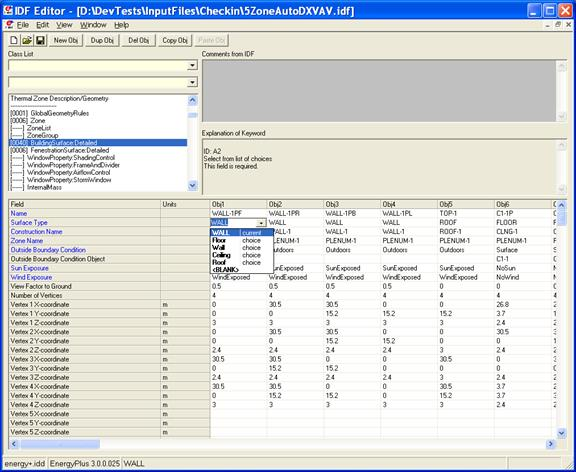
\includegraphics[width=0.9\textwidth, height=0.9\textheight, keepaspectratio=true]{media/image021.jpg}
\caption{IDF Editor Screen. \protect \label{fig:idf-editor-screen.}}
\end{figure}

\subsection{Start IDF Editor}\label{start-idf-editor}

IDF Editor should be located in the EnergyPlus\textbackslash{}PreProcessor\textbackslash{}IDFEditor directory where you installed EnergyPlus. By double clicking on the IDF Editor icon you will get a screen similar to the one shown above. IDF Editor works in conjunction with the current EnergyPlus Input Data Directory (IDD) file that resides in the directory where EnergyPlus is installed. Another way to start the IDF Editor is from EP-Launch. Multiple IDF files can be opened at once.

\subsection{Creating or Selecting an Input Data File}\label{creating-or-selecting-an-input-data-file}

Creating a new input data file or selecting an existing input data file can be accomplished either through use of the File menu on the menu bar at the top of the screen or through use of the New File icon button or Open File icon button on the tool bar.

\subsection{Class List}\label{class-list}

The class list shows how the items for the IDF are grouped.~ This class list follows the Data Dictionary (IDD) description. Select a class from the list by clicking on and highlighting the class. The field to the left of the selected class in the `Class List' will either contain {[}------{]} to indicate that this class has no objects in the IDF file or it will contain a number like {[}0003{]} to indicate the number of times the object currently appears in the IDF file. For example, for the BuildingSurface:Detailed class selected in the screen above under the Thermal Zone Description/Geometry group, there are 40 objects in the IDF file. The details for these 40 objects or any new object that is defined are displayed in columns within the grid. Each object is made up of fields and can be used to further define the object. Any units attached to each field are shown in the second column. You may need to scroll down the `field' list or maximize the application to see all of the fields. Likewise, you may need to scroll to the right of the main grid to see other objects.

Options under the view menu can change how you use the Class List. To display only classes that contain objects select the ``show classes with objects only'' option on the ``View'' menu. You can also toggle this feature on and off with CTRL+L. If the file is empty and has no objects, this toggle does not impact the display.

The ``Show Quick Select Dropdowns'' view menu option adds two new input fields to the main screen. The input fields can be used to go quickly to different classes in the main list of classes. By typing in the top input field, the group that start with those letters are displayed. After selecting one and pressing the tab button, classes in that group are shown and by typing the first few letters, you can easily select a specific class. Pressing tab again displays that class and it objects. This method allow for quick selection of classes if you remember the group name and class name.

\subsection{Changing Values}\label{changing-values}

By clicking and highlighting a value within an object, several things happen:

1)~~~Any user comments from the IDF file will be displayed in the `Comments from IDF' portion of the screen

2)~~~Any notes contained in the IDD for this input field will be displayed in the `Explanation of Keyword' portion of the screen

3)~~~The value can be edited. Depending on the field, a drop down list may display the default value, maximum and minimum, or other keywords that can be used with the field.

4)~~~Numeric fields that can be autosized will include ``autosize'' as a selection in the drop down list.

5)~~~Some numeric fields have a maximum and/or minimum value specified in the IDD. If the value entered is outside this range, the cell will be highlighted in pale orange.

6)~~~For values that are names of nodes, a new dialog box titled ``Edit or Select Node Name'' can be shown when the small button is pressed that is on the right side in each node name cell.

\subsection{Working with Objects}\label{working-with-objects}

To delete an object, first click on any value for the object and then click on the ``Del Obj'' button. To add a new object, click on the ``New Obj'' button and a new object column with fields set to blanks, zeros, or default values will be added to the far right of the grid. The ``Dup Obj'' button is similar to ``New Obj'', but copies the values of the fields of the currently selected object. Copying and pasting an object or groups of objects is also possible using the ``Copy Obj'' and ``Paste Obj'' buttons.~ These allow objects to be copied between files are also good for copying from files in the DataSets subdirectory. (Also see the Edit menu to perform these functions.)

\subsection{File Menu}\label{file-menu-000}

The File menu can be used for creating or selecting input files just like the buttons on the IDF Editor screen (see the \emph{Creating or Selecting an Input File} section above). In addition, the File menu is used to save a file or exit the IDF Editor. More than one file can be opened at a time.

The ``File'', ``Save Options'' screen is shown below.

~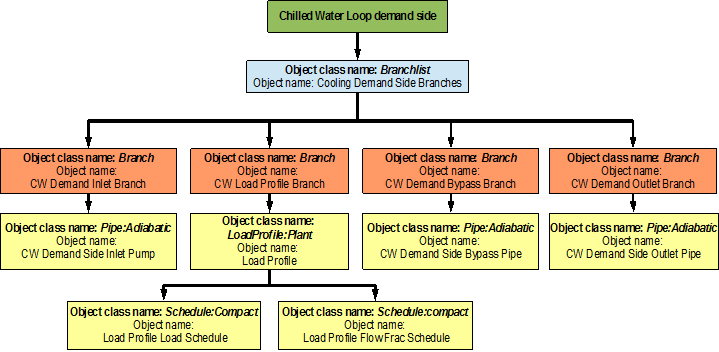
\includegraphics{media/image022.png}

Figure 22. IDF Editor Save Options Screen.

The save options allow the order of the objects in the file to be sorted by type of object or to keep the original order of the objects (for an existing file). The placement of new objects when the original order is specified can be either at the top or bottom of the file.

In addition, the Save Options also allow certain objects to be written to the file using a specific format that some users prefer. Selecting this option will format the following objects on a single line: Report, Report Meter, Report Variable, Version, Timestep in Hour, Inside Convection Algorithm, Outside Convection Algorithm, Solution Algorithm, Shadowing Calculations, Ground Reflectances, and GroundTemperatures:Deep. In addition, Schedule:Compact objects will be formatted to have two field for some lines. With this option, objects with geometric vertices are formatted to have the X, Y, and Z values on the same line. Those objects include: Surface:HeatTransfer, Surface:HeatTransfer:Sub, Surface:Shading:Detached:Fixed, Surface:Shading:Detached:Building and Surface:Shading:Attached.

The settings for the save options are kept for each file saved from the IDF Editor.

Also on the File menu is the Open DataSet menu and submenu. This allows you to open any input file that appears in the DataSet subdirectory and copy objects from them into another file. This is required because EnergyPlus does not read the DataSet files, it is up to you to include objects from them.

\subsection{Edit Menu}\label{edit-menu-000}

The Edit Menu offers options to create a new object, duplicate an object, and delete an object as well as finding and searching. The object options are the same operations as can be accomplished by using the `New Obj', `Dup Obj' and `Del Obj' buttons (see the \emph{Working with Objects} section above). In addition, the ``Next Row after Enter'' option can be toggled. When this option is on, the selection moves down one row after pressing Enter. The copy and paste object commands allow a single object to be copied within a file or between files. The pasted object appears as the last object in the class. This capability makes it easier to utilize the data in the DataSets directory. The Find Class and Search and Replace options can be used to search through the list of classes or the values of a file quickly. If renaming objects, the recommended approach is to rename the object and select the cell again and open the Search and Replace dialog. This will show other places in the file that use that object name that also may need to be changed.

\subsection{View Menu}\label{view-menu-000}

The View menu offers options for units and column widths. The Narrow/Medium/Wide Column options set the standard column width for items in the object grid. Individual columns can also be resized by dragging the column separator. The displayed value is rounded and/or expressed in scientific notation to fit within the column width.

EnergyPlus input files must always be in SI units. Selecting ``Inch-Pound'' (IP) units in the View menu displays and edits values in IP units.

1)~~~The IP unit will be displayed in the units column of the object grid. Some SI units convert to multiple IP units. For example, W becomes Btu/hr for heating and cooling capacity but remains as W for lighting and electrical equipment.

2)~~~All conversion factors used in the IDF editor are documented in a block of comments near the top of the Energy+.IDD file.

3)~~~Schedules, fluid properties and curves now support IP unit conversions. For curves, the minimum and maximum values are converted but the coefficients are not.

To display only classes that contain objects select the ``show classes with objects only'' option on the ``View'' menu. You can also toggle this feature on and off with CTRL+L. If the file is empty and has no objects, this toggle does not impact the display.

The ``Show Quick Select Dropdowns'' view menu option adds two new input fields to the main screen. The input fields can be used to go quickly to different classes in the main list of classes.

The ``Validity Check'' function has replaced and expanded upon the old~ ``Check Out-of-Range'' function. It can also be started by using CTRL-R. The ``Validity Check'' function performs three kinds of validity checks. It displays the values and locations for objects with values that are either above the maximum or below the minimum values.~ It also displays fields that contain invalid references. The ``Validity Check'' dialog also shows when an entry for a field is not one of the possible lists of choices. The Perform Validity Check When Saving File can be turned on and off and automatically performs the check whenever the file is saved.

\subsection{Help Menu}\label{help-menu-000}

The Help menu offers options to open the EnergyPlus documentation files.


\chapter{Other Useful programs/information}\label{other-useful-programsinformation}


\section{HVACTemplate Objects}\label{hvactemplate-objects}

HVAC Template objects are available. These are intended to allow for several ``usual'' HVAC types to be expanded into EnergyPlus HVAC inputs with minimal user entries. These are described in the ``Input/Output Reference'' document under the Group ``HVACTemplates'' and the expansion process is described in the Auxiliary Programs document under ``ExpandObjects''.


\chapter{Data Sets}\label{data-sets}

Data sets are the EnergyPlus answer to ``libraries''. Data sets come in two flavors -- a simple list and a ``macroized'' list. Macroized lists are files that could have the elements extracted using a simple macro name.

\section{Simple List Data Sets}\label{simple-list-data-sets}

\subsection{AirCooledChillers.idf}\label{aircooledchillers.idf}

This dataset includes performance curves for air cooled electric EIR chiller (object type: Chiller:Electric:EIR). Knowing the type of chiller that you want to simulate, you can find it and the associated performance curves in the dataset file. A brief synopsis of AirCooledChiller.idf is shown below:

\begin{lstlisting}

! AirCooledChillers.idf
  !
  ! This dataset includes performance curves for object type Chiller:Electric:EIR
  !
  ! Summary Table for Electric EIR Chiller reference data sets.
  ! Chillers are listed in order of reference capacity. Reference capacity and COP do not necessarily
  ! indicate rated capacity and COP at standard rating conditions (e.g. ARI Standard 550/590).
  !
  ! Performance curves developed from information collected from manufacturer's catalog data
  ! The nomenclature used for the chiller is as follows:
  ! ElectricEIRChiller - Manufacturer's Name - Model - Reference Capacity in kW - Reference COP
  !
  !                                                      Compressor   Reference    Reference
  ! Chiller Name                                            Type       Capacity      COP
  !                                                                    kW (tons)
  ! ElectricEIRChiller McQuay AGZ010BS 34.5kW/2.67COP      Scroll     34.5 (9.8)      2.67
  ! ElectricEIRChiller McQuay AGZ013BS 47.1kW/2.67COP      Scroll     47.1 (13.4)     2.67
  ! ElectricEIRChiller York YCAL0019EE 54.2kW/2.9COP       Scroll     54.2 (15.4)     2.9
  ! ElectricEIRChiller McQuay AGZ017BS 54.5kW/2.67COP      Scroll     54.5 (15.5)     2.67
\end{lstlisting}

\subsection{ASHRAE\_2005\_HOF\_Materials.idf}\label{ashraeux5f2005ux5fhofux5fmaterials.idf}

This reference data set contains content from two chapters in the ASHRAE 2005 Handbook of Fundamentals, Chapter 30 - the Cooling and Heating Loads calculations chapter has both materials with thermal properties and constructions for Light, Medium, and Heavy buildings. Chapter 25 contains details thermal properties of many materials -- no constructions are created from that data.

The following materials and constructions are created from ASHRAE Handbook of Fundamentals, 2005, Chapter 30, Table 19 and Table 22. These are representative of materials and constructions used in Cooling and Heating Load Calculations.

\subsection{Boilers.idf}\label{boilers.idf}

This dataset includes performance curves for non-electric boilers. Reference: Condensing Technology, Technical Series, Viessmann, 9446 803 - 1 GB Nov. 2004.

\subsection{California\_Title\_24-2008.idf}\label{californiaux5ftitleux5f24-2008.idf}

This dataset includes occupancy data and non-residential schedules for California Title 24-2008 compliance calculations when lighting plans are submitted for the Entire Building or when lighting compliance is not performed. Data is based on Table N2-5 of the 2008 Non-residential ACM Manual.

\subsection{Chillers.idf}\label{chillers.idf}

This dataset includes object types for specific (by manufacturer and type) Chiller:Electric:EIR and Chiller: Electric:ReformulatedEIR and associated performance curves.

Knowing the type of chiller that you want to simulate, you can find it and the associated performance curves in the dataset file. By example, here is part of the comments in the Chiller.idf file:

\begin{lstlisting}

! Summary Table for Electric EIR Chiller reference data sets (Ref. CoolTools project).
  ! Chillers are listed in order of compressor type and reference capacity (model calibration
  ! point). Reference capacity and COP do not necessarily indicate rated capacity and COP at
  ! standard rating conditions (e.g. ARI Standard 550/590).
  !
  ! Performance curves developed from information collected over a 10-year period from 1991 to 2001.
  !
  !                                                      Compressor   Reference  Reference Unloading
  ! Chiller Name                                            Type       Capacity    COP     Mechanism
  !                                                                    kW (tons)
  !-------------------------------------------------------------------------------------------------
  ! ElectricEIRChiller McQuay WSC 471kW/5.89COP/Vanes    Centrifugal   471 (134)   5.89   Inlet Vanes
  ! ElectricEIRChiller York YT 563kW/10.61COP/Vanes      Centrifugal   563 (160)   10.61  Inlet Vanes
  ! ElectricEIRChiller McQuay PEH 703kW/7.03COP/Vanes    Centrifugal   703 (200)   7.03   Inlet Vanes
  ! ElectricEIRChiller Carrier 23XL 724kW/6.04COP/Vanes  Centrifugal   724 (206)   6.04   Inlet Vanes
\end{lstlisting}

\subsection{CompositeWallConstructions.idf}\label{compositewallconstructions.idf}

The Reference Data Set CompositeWallConstructions.idf contains constructions and associated materials for a set of \textbf{composite} walls. These are walls---such as stud walls---that have complicated heat-flow paths so that the conduction is two- or three-dimensional.

An example entry in this data set--for an insulated 2''x4'' steel-stud wall--looks like:

\begin{lstlisting}

CONSTRUCTION,Composite 2x4 Steel Stud R11,
  ! ASHRAE 1145-RP Wall Assembly 10
  ! 2"x4" steel studs at 24" on center with between-stud R11 fibreglass insulation.
  ! Studs are 3.5", 16 gauge, 15 flange.
  ! Layers are 1/2" wood siding, 1/2" plywood, 2x4 steel studs and R11 insulation, 1/2" gypsum board.
  ! Area-average R-Value = 8.796 ft2-F-h/Btu (1.548 m2-K/W).
  ! Total wall thickness = 5.00in (0.127m)
  ! Material layer names follow:
    Composite 2x4 Steel Stud R11 \#3,
    Composite 2x4 Steel Stud R11 \#2,
    Composite 2x4 Steel Stud R11 \#1;
  MATERIAL,Composite 2x4 Steel Stud R11 \#1,
    Smooth,  !- Roughness
    0.013,   !- Thickness (m)
    0.720,   !- Conductivity (W/m-K)
    640.0,   !- Density (kg/m3)
    1048,    !- Specific Heat (J/kg-K)
    0.9,     !- Absorptance:Thermal
    0.7,     !- Absorptance:Solar
    0.7;     !- Absorptance:Visible
  MATERIAL,Composite 2x4 Steel Stud R11 \#2,
    Smooth,  !- Roughness
    0.089,   !- Thickness (m)
    0.060,   !- Conductivity (W/m-K)
    118.223, !- Density (kg/m3)
    1048,    !- Specific Heat (J/kg-K)
    0.9,     !- Absorptance:Thermal
    0.7,     !- Absorptance:Solar
    0.7;     !- Absorptance:Visible
  MATERIAL,Composite 2x4 Steel Stud R11 \#3,
    Smooth,  !- Roughness
    0.025,   !- Thickness (m)
    0.452,   !- Conductivity (W/m-K)
    413.782, !- Density (kg/m3)
    1048,    !- Specific Heat (J/kg-K)
    0.9,     !- Absorptance:Thermal
    0.7,     !- Absorptance:Solar
    0.7;     !- Absorptance:Visible
\end{lstlisting}

The materials here are \textbf{not} real materials but are ``equivalent'' materials obtained from finite-difference modeling. The thickness, conductivity, density and specific heat values of the material layers for the different constructions have been taken from the ASHRAE report ``Modeling Two- and Three-Dimensional Heat Transfer through Composite Wall and Roof Assemblies in Hourly Energy Simulation Programs (1145-TRP),'' by Enermodal Engineering Limited, Oak Ridge National Laboratory, and the Polish Academy of Sciences, January 2001. EnergyPlus will calculate conduction transfer functions using these materials. The heat transfer based on these conduction transfer functions will then be very close to what would be calculated with a two- or three-dimensional heat transfer calculation.

For stud walls, using these composite constructions will give more accurate heat flow than you would get by manually dividing the wall into a stud section and a non-stud section.

If your wall's exterior or interior roughness or thermal, solar or visible absorptances are different from those in the data set, you can make the appropriate changes to the first material (the outside layer) or the third material (the inside layer). \textbf{None of the other values should be changed.}

Following is a summary of the constructions in the composite wall data set:

\begin{lstlisting}

CONSTRUCTION,Composite 2x4 Wood Stud R11,
  ! ASHRAE 1145-RP Wall Assembly 1
  ! 2"x4" wood studs at 24" on center with between-stud R11 fibreglass insulation.
  ! Layers are 1/2" wood siding, 1/2" plywood, 2x4 wood studs and R11 insulation, 1/2" gypsum board.
  ! Area-average R-Value = 11.391 ft2-F-h/Btu (2.005 m2-K/W).

  CONSTRUCTION,Composite 2x6 Wood Stud R19,
  ! ASHRAE 1145-RP Wall Assembly 2
  ! 2"x6" wood studs at 24" on center with between-stud R19 fibreglass insulation.
  ! Layers are 1/2" wood siding, 1/2" plywood, 2x6 wood studs and R19 insulation, 1/2" gypsum board.
  ! Area-average R-Value = 17.487 ft2-F-h/Btu (3.078 m2-K/W).

  CONSTRUCTION,Composite Insulated Concrete Form Wall With Steel Ties,
  ! ASHRAE 1145-RP Wall Assembly 7
  ! Wall system is made of two rigid insulation sides held together with wire mesh.
  ! The two sides come together to create the formwork for the concrete.
  ! Layers are 3/4" concrete stucco, outer polystyrene shell, concrete core, inner polystyrene shell.
  ! Area-average R-Value = 11.230 ft2-F-h/Btu (1.977 m2-K/W).

  CONSTRUCTION,Composite Concrete/Foam/Concrete With Steel Connectors,
  ! ASHRAE 1145-RP Wall Assembly 8
  ! Wall system is made of two 3" concrete slabs separated by 2" rigid insulation.
  ! The slab connectors are steel ties with a 0.15"x0.15" cross section.
  ! Layers are 3" concrete, 2" polystyrene, 3" concrete.
  ! Area-average R-Value = 7.659 ft2-F-h/Btu (1.348 m2-K/W).

  CONSTRUCTION,Composite Concrete/Foam/Concrete With Plastic Connectors,
  ! ASHRAE 1145-RP Wall Assembly 9
  ! Wall system is made of two 3" concrete slabs separated by 2" rigid insulation.
  ! The slab connectors are plasic ties with a 0.25"x0.25" cross section.
  ! Layers are 3" concrete, 2" polystyrene, 3" concrete.
  ! Area-average R-Value = 10.582 ft2-F-h/Btu (1.862 m2-K/W).

  CONSTRUCTION,Composite 2x4 Steel Stud R11,
  ! ASHRAE 1145-RP Wall Assembly 10
  ! 2"x4" steel studs at 24" on center with between-stud R11 fibreglass insulation.
  ! Studs are 3.5", 16 gauge, 15 flange.
  ! Layers are 1/2" wood siding, 1/2" plywood, 2x4 steel studs and R11 insulation, 1/2" gypsum board.
  ! Area-average R-Value = 8.796 ft2-F-h/Btu (1.548 m2-K/W).

  CONSTRUCTION,Composite Brick Foam 2x4 Steel Stud R11,
  ! ASHRAE 1145-RP Wall Assembly 15
  ! Brick veneer, polystyrene, 2"x4" steel studs at 24" on center with
  !  between-stud R11 fibreglass insulation.
  ! Studs are 3.5", 16 gauge, 15 flange.
  ! Layers are 3.25" brick,1" polystyrene insulation, 1/2" plywood, 2x4 steel studs and R11 insulation,
  !  1/2" gypsum board.
  ! Area-average R-Value = 12.792 ft2-F-h/Btu (2.251 m2-K/W).

  CONSTRUCTION,Composite 2x6 Steel Stud R19,
  ! ASHRAE 1145-RP Wall Assembly 16
  ! 2"x6" steel studs at 24" on center with between-stud R19 fibreglass insulation.
  ! Studs are 5.5", 16 gauge, 15 flange.
  ! Layers are 1/2" wood siding, 1/2" plywood, 2x6 steel studs and R19 insulation, 1/2" gypsum board.
  ! Area-average R-Value = 12.792 ft2-F-h/Btu (1.991 m2-K/W).

  CONSTRUCTION,Composite Foam 2x6 Steel Stud R19,
  ! ASHRAE 1145-RP Wall Assembly 17
  ! Polystyrene, 2"x6" steel studs at 24" on center with between-stud R19 fibreglass insulation.
  ! Studs are 5.5", 16 gauge, 15 flange.
  ! Layers are 3/4" concrete stucco,1" polystyrene insulation, 1/2" plywood, 2x6 steel studs and R19 insulation,
  !  1/2" gypsum board.
  ! Area-average R-Value = 15.157 ft2-F-h/Btu (2.668 m2-K/W).

  CONSTRUCTION,Composite Brick Foam 2x6 Steel Stud R19,
  ! ASHRAE 1145-RP Wall Assembly 18
  ! Brick veneer, polystyrene, 2"x6" steel studs at 24" on center with
  !  between-stud R19 fibreglass insulation.
  ! Studs are 5.5", 16 gauge, 15 flange.
  ! Layers are 3.25" brick,1" polystyrene insulation, 1/2" plywood, 2x6 steel studs and R19 insulation,
  !  1/2" gypsum board.
  ! Area-average R-Value = 15.465 ft2-F-h/Btu (2.722 m2-K/W).

  CONSTRUCTION,Composite 2-Core Filled Concrete Block Uninsulated,
  ! ASHRAE 1145-RP Wall Assembly 19
  ! Wall system is made of 12" 2-core concrete blocks without insulation.
  ! The core area is filled with rebar and poured concrete.
  ! Area-average R-Value = 1.326 ft2-F-h/Btu (0.239 m2-K/W).

  CONSTRUCTION,Composite 2-Core Filled Concrete Block Insulated,
  ! ASHRAE 1145-RP Wall Assembly 20
  ! Wall system is made of 12" 2-core concrete blocks with 1.875"-thick
  !  foam inserts in the block cores.
  ! The remaining core area is filled with poured concrete.
  ! Area-average R-Value = 2.291 ft2-F-h/Btu (0.403 m2-K/W).
\end{lstlisting}

\subsection{DXCoolingCoil.idf}\label{dxcoolingcoil.idf}

This dataset includes performance curves for the object types Coil:Cooling:DX:SingleSpeed and Coil:Cooling:DX:TwoStageWithHumidityControlMode. This data set is developed by using catalog data published by different manufacturers which are listed in the file.

Here is a synopsis of the DXCoolingCoil.idf:

\begin{lstlisting}

! DXCoolingCoil.idf
  !
  ! This dataset includes performance curves for the object types Coil:Cooling:DX:SingleSpeed and
  ! Coil:Cooling:DX:TwoStageWithHumidityControlMode
  !
  ! Reference capacity at standard rating conditions (ARI 95F OAT, 67F EWBT and air flow rate
  ! around 400 cfm/Ton).
  !
  ! In the objects Coil:Cooling:DX:SingleSpeed and Coil:Cooling:DX:TwoStageWithHumidityControlMode
  ! below, input fields 'Availability Schedule Name', 'Air Inlet Node Name' and 'Air Outlet Node
  ! Name' need to be defined by the user.
  !
  !------------------------------------------------------------------------------------------------!                             Compressor  Nominal    Reference      Reference   Refrig  Expansion
  !                                                                                         Valve
  ! Name                           Type     Capacity   Capacity          COP       Type      Type
  !                                         (tons)     kW (tons)
  !------------------------------------------------------------------------------------------------! Carrier Centurion 50PG06      Scroll      5        18.28(5.2)        4.15     R-410A    TXV
  ! Carrier Centurion 50PG12      Scroll      10       36.79(10.47)      4.05     R-410A    TXV
  ! Carrier Centurion 50PG24      Scroll      20       73.81(21)         3.95     R-410A    TXV

    Coil:Cooling:DX:SingleSpeed,
      Carrier Centurion 50PG06,     !- Name
      CoolingCoilAvailSched,        !- Availability Schedule Name
      18276.96,                     !- Rated Total Cooling Capacity {W}
      0.74,                         !- Rated Sensible Heat Ratio
      4.15,                         !- Rated COP
      0.944,                        !- Rated Air Flow Rate {m3/s}
      ,                             !- Rated Evaporator Fan Power Per Volume Flow Rate {W/(m3/s)}
      DXCoilAirInletNode,           !- Air Inlet Node Name
      DXCoilAirOutletNode,          !- Air Outlet Node Name
      CarrierCenturion50PG06CapFT,  !- Total Cooling Capacity Function of Temperature Curve Name
      CarrierCenturion50PG06CapFFF, !- Total Cooling Capacity Function of Flow Fraction Curve Name
      CarrierCenturion50PG06EIRFT,       !- Energy Input Ratio Function of Temperature Curve Name
      CarrierCenturion50PG06EIRFFF,      !- Energy Input Ratio Function of Flow Fraction Curve Name
      Carrier Centurion 50PG06 PLFFPLR;  !- Part Load Fraction Correlation Curve Name

  ! Curve set (5 Curves):

  ! Cooling Capacity Function of Temperature Curve
  ! x = Entering Wet-bulb Temp and y = Outdoor Dry-bulb Temp

    Curve:Biquadratic,
      CarrierCenturion50PG06CapFT,  !- Name
      0.9953455,               !- Coefficient1 Constant
      -0.0118418,              !- Coefficient2 x
      0.0012277,               !- Coefficient3 x**2
      0.0030246,               !- Coefficient4 y
      -0.0000702,              !- Coefficient5 y**2
      -0.0003685,              !- Coefficient6 x*y
      12.22,                   !- Minimum Value of x
      26.67,                   !- Maximum Value of x
      15.56,                   !- Minimum Value of y
      51.67,                   !- Maximum Value of y
      ,                        !- Minimum Curve Output
      ,                        !- Maximum Curve Output
      Temperature,             !- Input Unit Type for X
      Temperature,             !- Input Unit Type for Y
      Dimensionless;           !- Output Unit Type

  ! EIR Function of Temperature Curve
  ! x = Entering Wet-bulb Temp and y = Outdoor Dry-bulb Temp

    Curve:Biquadratic,
      CarrierCenturion50PG06EIRFT,  !- Name
      0.3802131,               !- Coefficient1 Constant
      0.0199468,               !- Coefficient2 x
      -0.0006682,              !- Coefficient3 x**2
      0.0058933,               !- Coefficient4 y
      0.0004646,               !- Coefficient5 y**2
      -0.0004072,              !- Coefficient6 x*y
      12.22,                   !- Minimum Value of x
      26.67,                   !- Maximum Value of x
      15.56,                   !- Minimum Value of y
      51.67,                   !- Maximum Value of y
      ,                        !- Minimum Curve Output
      ,                        !- Maximum Curve Output
      Temperature,             !- Input Unit Type for X
      Temperature,             !- Input Unit Type for Y
      Dimensionless;           !- Output Unit Type

  ! Cooling Capacity Function of Flow Fraction Curve
  ! x = Flow Fraction

    Curve:Quadratic,
      CarrierCenturion50PG06CapFFF,  !- Name
      0.7705358,               !- Coefficient1 Constant
      0.2848007,               !- Coefficient2 x
      -0.0580891,              !- Coefficient3 x**2
      0.75,                    !- Minimum Value of x
      1.25;                    !- Maximum Value of x

  ! EIR Function of Flow Fraction Curve
  ! x = Flow Fraction

    Curve:Quadratic,
      CarrierCenturion50PG06EIRFFF,   !- Name
      1.3439758,               !- Coefficient1 Constant
      -0.5111244,              !- Coefficient2 x
      0.1732549,               !- Coefficient3 x**2
      0.75,                    !- Minimum Value of x
      1.25;                    !- Maximum Value of x

  ! Part Load Fraction Function of Part Load Ratio Curve
  ! x = Part Load Ratio

    Curve:Quadratic,
      CarrierCenturion50PG06PLFFPLR,   !- Name
      0.85,                    !- Coefficient1 Constant
      0.15,                    !- Coefficient2 x
      0.0,                     !- Coefficient3 x**2
      0.0,                     !- Minimum Value of x
      1.0;                     !- Maximum Value of x
\end{lstlisting}

\subsection{ElectricGenerators.idf}\label{electricgenerators.idf}

This dataset includes inputs for the GENERATOR:MICROTURBINE object and associated performance curves. The performance curves were developed from manufacturer data collected in Summer 2007.

Includes data for generators: Capstone C65, Elliott TA100,~ Ingersoll Rand MT70, Ingersoll Rand MT250.

Further documentation is contained in the dataset file.

\subsection{Electricity USA Environmental Impact Factors.idf}\label{electricity-usa-environmental-impact-factors.idf}

United States 1999 national average electricity emissions factors based on eGRID, 1605, AirData. United States Water Emission Fuel Factors are the combined thermoelectric and hydroelectric weighted averages from:

Torcellini, Paul; Long, Nicholas; Judkoff, Ron; ``Consumptive Water Use for U.S. Power Production'';NREL Report No. TP-550-33905. Golden, CO; 2003; \url{http://www.nrel.gov/docs/fy04osti/33905.pdf};

or

Torcellini, Paul; Long, Nicholas; Judkoff, Ron; ``Consumptive Water Use for U.S. Power Production''; ASHRAE Transactions 2003, Vol 110, Part 1. Atlanta, GA; January 2004;

\subsection{ElectronicEnthalpyEconomizerCurves.idf}\label{electronicenthalpyeconomizercurves.idf}

These curves approximate the electronic (variable) enthalpy curves used to simulate humidity biased economizer control. This control scheme adjusts the upper outdoor air humidity ratio based on outdoor air dry-bulb temperature as shown in the figure below. California Title 24 ACM 2005 lists the optional economizer control strategies. One of these control strategies is referred to as variable enthalpy control curve A. This control strategy is also cited in ASHRAE Standard 90.1-2004, using the term ``electronic enthalpy''. Electronic enthalpy curves A-D are included in this dataset.

\begin{figure}[hbtp] % fig 12
\centering
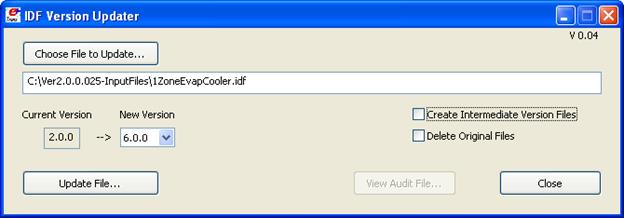
\includegraphics[width=0.9\textwidth, height=0.9\textheight, keepaspectratio=true]{media/image027.jpg}
\caption{Psychrometric Chart Illustration of the Electronic (Variable) Enthalpy Economizer Limit Example Curve Objects \protect \label{fig:psychrometric-chart-illustration-of}}
\end{figure}

For the curves provided, curve A has the highest limit and curve D has the lowest limit. These curve objects represent a single-point electronic enthalpy control curve with the curve object's minimum value of x (temperature) crossing the psychrometric chart's saturation line and the curve object's maximum value of x crossing the psychrometric chart's dry-bulb temperature axis. The curve object's minimum (maximum) value of x should be just low (high) enough to ensure that the curve crosses the psychrometric chart's saturation line (temperature axis). The curves are evaluated at an outdoor dry-bulb temperature to provide a maximum operating outdoor humidity ratio for economizer operation. If the outdoor humidity ratio is greater than this maximum value, economizer operation is terminated. These curves may be used with other economizer limits to create multi-point economizer control (Temperature Limit, Temperature Low Limit, Enthalpy Limit, and Dewpoint Temperature Limit).

\subsubsection{Form of the Electronic Enthalpy Curve Equation:}\label{form-of-the-electronic-enthalpy-curve-equation}

The electronic enthalpy curve equation represents a unique curve and is a function of both temperature and relative humidity. The equation is set equal to a constant which provides a unique temperature for each relative humidity entered into the equation. Each control curve has a unique constant as shown in the table below. Other constants may be used to develop specialized electronic enthalpy curves.

\begin{equation}
K = 45.672192 - 1.1559942 \cdot T - 0.144599 \cdot RH
\end{equation}

where:

\begin{itemize}
\tightlist
\item
  K~ = Constant value to represent specific curve
\item
  T~ = Outdoor Dry-Bulb Temperature (C)
\item
  RH = Outdoor Relative Humidity (\%)
\end{itemize}

NOTE:~ modifying the RH multiplier (-0.144599) tends to ``wag'' the curvature at the upper relative humidities. Decreasing the multiplier ``wags'' the upper portion of the curve downward, increasing ``wags'' it upwards. Modifying the constant (K) moves the intersection of the curve with the Dry-Bulb Temperature ~axis. Increasing the constant moves the intersection to the left as shown in the figure, decreasing moves to the right. The minimum and/or maximum x boundaries in the curve objects may have to be adjusted when modifying the equation.

% table 43
\begin{longtable}[c]{p{1.5in}p{1.5in}p{3.0in}}
\caption{Electronic Enthalpy Curve Constants and approximate control point at 50\% RH \label{table:electronic-enthalpy-curve-constants}} \tabularnewline
\toprule 
Control Curve & Curve Constant K & Approximate Control Point at 50\% RH (ºC) \tabularnewline
\midrule
\endfirsthead

\caption[]{Electronic Enthalpy Curve Constants and approximate control point at 50\% RH} \tabularnewline
\toprule 
Control Curve & Curve Constant K & Approximate Control Point at 50\% RH (ºC) \tabularnewline
\midrule
\endhead

A & 12 & 22.9 \tabularnewline
B & 14 & 21.1 \tabularnewline
C & 16 & 19.4 \tabularnewline
D & 18 & 17.7 \tabularnewline
\bottomrule
\end{longtable}

\subsubsection{Example Curve A:}\label{example-curve-a}

The method described here was used to create each of the four ``cubic'' curve objects provided in the electronic enthalpy economizer control data set.

\textbf{Step 1:} Substitute the curve constant K for curve A (12) into the electronic enthalpy curve equation and solve for temperature. Then identify the outdoor air dry-bulb temperatures at known values of relative humidity (e.g., columns 1 and 2 in the table below). Psychrometric routines are helpful for this step.

\begin{equation}
\text{Temperature} = \frac{12 - 45.672192 + 0.144599 \cdot \text{RelativeHumidity}}{-1.1559942}
\end{equation}

\textbf{Step 2:} Identify humidity ratio at each point (e.g.~column 3 in the following table). Psychrometric routines are helpful for this step.

\begin{longtable}[c]{p{1.78in}p{1.5in}p{2.71in}}
\toprule 
Relative Humidity (\%) & Temperature (ºC) & Calculated Humidity Ratio (kg/kg) \tabularnewline
\midrule
\endfirsthead

\toprule 
Relative Humidity (\%) & Temperature (ºC) & Calculated Humidity Ratio (kg/kg) \tabularnewline
\midrule
\endhead

0 & 29.128 & 0.00000 \tabularnewline
10 & 27.877 & 0.00232 \tabularnewline
20 & 26.627 & 0.00433 \tabularnewline
30 & 25.376 & 0.00605 \tabularnewline
40 & 24.125 & 0.00750 \tabularnewline
50 & 22.874 & 0.00872 \tabularnewline
60 & 21.623 & 0.00971 \tabularnewline
70 & 20.372 & 0.01051 \tabularnewline
80 & 19.121 & 0.01112 \tabularnewline
90 & 17.871 & 0.01158 \tabularnewline
100 & 16.620 & 0.01189 \tabularnewline
\bottomrule
\end{longtable}

\textbf{~}

\textbf{Step 3:} Use multiple linear regression to solve one of the following equations:

\emph{Quadratic~ Curve}: Humidity Ratio = A0 + A1*Temperature + A2*Temperature\(^{2}\)

\emph{Cubic~ Curve}: Humidity Ratio = A0 + A1*Temperature + A2*Temperature\(^{2}\) + A3*Temperature\(^{3}\)

\textbf{Step 4:} Use the coefficients calculated in the multiple linear regression to create a cubic (or quadratic) curve object.

\subsection{Exhaust Fired Chiller.idf}\label{exhaust-fired-chiller.idf}

This dataset includes the curves for exhaust fired absorption chiller.

1)~~~Cooling Capacity Function of Temperature Curve

2)~~~Thermal Energy Input to Cooling Output Ratio Function of Temperature Curve

3)~~~Thermal Energy Input to Cooling Output Ratio Function of Part Load Ratio Curve

\subsection{Fossil Fuel Environmental Impact Factors.idf}\label{fossil-fuel-environmental-impact-factors.idf}

Impact factors for environmental reporting. References for each fuel are given in the dataset.

\subsection{FluidPropertiesRefData.idf}\label{fluidpropertiesrefdata.idf}

This data set includes fluid properties reference data. Fluid properties for R404a, R407a, R410a, R505a, R744, were developed using the NIST Standard Reference Database 23, NIST Reference Thermodynamic and Transport Properties -- REFPROP, April 2007 Version 8.0, National Institute of Standards and Technology, 2007. The other refrigerants were developed using older versions of the NIST Standard Reference Database. The entire data set includes:

\begin{longtable}[c]{@{}l@{}}
\toprule 
Refrigerants \tabularnewline
\midrule
\endfirsthead

\toprule 
Refrigerants \tabularnewline
\midrule
\endhead

R11 \tabularnewline
R12 \tabularnewline
R22 \tabularnewline
R123 \tabularnewline
R134a \tabularnewline
R404a \tabularnewline
R410a \tabularnewline
R507a \tabularnewline
NH3 \tabularnewline
Steam \tabularnewline
R744 \tabularnewline
\bottomrule
\end{longtable}

To use the data, copy the appropriate data for the refrigerant you desire into your input file.

\subsection{GlycolPropertiesRefData.idf}\label{glycolpropertiesrefdata.idf}

This data set includes fluid properties (glycol) reference data. Reference for the data is the ASHRAE Handbook of Fundamentals. Included are:

\begin{longtable}[c]{@{}l@{}}
\toprule 
Glycols \tabularnewline
\midrule
\endfirsthead

\toprule 
Glycols \tabularnewline
\midrule
\endhead

EthyleneGlycol \tabularnewline
PropyleneGlycol \tabularnewline
Water \tabularnewline
\bottomrule
\end{longtable}

To use the data, copy the appropriate data for the glycol you desire into your input file.

\subsection{GHLERefData.idf}\label{ghlerefdata.idf}

This file contains sample input for the ground loop heat exchanger model. The response of the borehole/ground is found from the `G-function' that is~ defined in the input as series of `n' pairs of values (LNTTSn, GNFCn). It is important to note that the G-functions have to be calculated for specific GHE configurations and borehole resitance, length and borehole/ length ratio. That is, the parameters for the units vary with each design. The data in this file are intended as examples/samples and may not represent actual designs.

The sample data has been calculated for a number of configurations:

\begin{itemize}
\tightlist
\item
  1 x 2 boreholes
\item
  4 x 4 boreholes
\item
  8 x 8 boreholes
\end{itemize}

Data is given for both `standard' grout (k = 0.744 W/m.K) and `thermally enhanced' grout (k = 1.471 W/m.K). The flow rate per borehole is .1514 kg/s. The pipe given is 0.75in. Dia. SDR11 HDPE. The fluid is water. The borehole/length ratio is 0.06~ (76.2m/4.572m {[}300ft/15ft{]})

\subsection{MoistureMaterials.idf}\label{moisturematerials.idf}

This data set includes the special moisture materials that can be used with the Moisture Penetration Depth Conduction Transfer Function (EMPD) and Combined Heat and Moisture Finite Element (HAMT) calculation procedures.

\subsection{PerfCurves.idf}\label{perfcurves.idf}

This file contains performance curves for various EnergyPlus equipment objects.

\begin{itemize}
\item
  Variable speed DX cooling:~ These curves are appropriate for small DX cooling units with variable speed compressors. These curves would be referenced by the EnergyPlus object Coil:Cooling:DX:TwoSpeed. See the example input file 5ZoneAutoDXVAV for an example of their use.
\item
  Variable Speed Cooling Tower: These model coefficient objects are appropriate for use with the variable speed cooling tower object and represent the coefficients used in the YorkCalc and CoolTools empirical models. These model coefficient objects would be referenced by the EnergyPlus object Cooling Tower:Variable Speed. See the example input file CoolingTower\_VariableSpeed.idf for an example of where these curves could be used (these model coefficient objects are not specifically used in this idf but could be used by the Cooling Tower:Variable Speed object). Additional information on variable speed cooling tower model coefficients can be found in the Input Output Reference and Engineering Reference documents.
\item
  Note that performance curves for the Electric EIR chiller and the Electric Reformulated EIR chiller are contained in the Chillers.idf dataset.
\end{itemize}

\subsection{PrecipitationSchedulesUSA.idf}\label{precipitationschedulesusa.idf}

This file contains schedules (for an entire year) of precipitation for use with the SitePrecipitation object. Use these schedules for adding rain water to the simulation. The values are in meters per hour and are scaled to match the average monthly precipitation. They also coincide with the EPW rain/snow flags from the original source files.

\subsection{RefrigerationCasesDataSet.idf}\label{refrigerationcasesdataset.idf}

All the refrigerated cases included in this database are listed in the following list. Comments before each refrigeration:case object include the manufacturer's model number and assumptions about the fan, lights, defrost etc. The user must ensure that the case names used in the idf file are UNIQUE and must supply the correct zone name.~ The user must also supply any required correction curves or schedules. The defrost and drip-down schedule names included here indicate the frequency and duration required. The user must ensure that schedules are provided that meet these needs and that are diversified so that all the cases don't start their defrost cycles at the same time. Please see the example cases for supermarkets to see how these case objects are included with the rest of a supermarket refrigeration system.

\begin{itemize}
\item
  Multi-Deck Dairy/Deli Merchandiser with Synergy-E
\item
  Multi-Deck Rear Dairy/Deli Merchandiser with Synergy-E
\item
  Multi-Deck Deli back
\item
  Single Deck Club Case Merchandiser
\item
  Single Deck Club Case Merchandiser
\item
  Single Deck Club Merchandiser
\item
  Single Deck Club Case Merchandiser
\item
  Multi-Deck Produce/Dairy/Deli/Meat/Seafood Merchandiser
\item
  Multi-Deck Dairy/Deli Merchandiser with Synergy-E
\item
  Multi Deck Frozen Food Merchandiser
\item
  Multi Deck Frozen Food Merchandiser
\item
  Multi-Deck Produce/Dairy/Deli/Meat/Seafood Merchandiser
\item
  Wide Island Multi-Deck Deli/Meat Merchandiser
\item
  Wide Island Multi-Deck Deli/Meat Merchandiser
\item
  International Style Service Deli/Meat/Seafood Merchandiser
\item
  International Style Flat Glass Service Deli/Meat/Seafood Merchandiser
\item
  Multi-Deck Produce/Dairy/Deli/Meat/Seafood Merchandiser
\item
  Multi-Deck Deli/Meat End Cap Merchandiser
\item
  Multi-Deck Produce/Dairy/Deli Merchandiser
\item
  Multi-Deck Produce/Dairy/Deli/Meat/Seafood Merchandiser
\item
  Multi-Deck Dairy/Deli/Produce/Meat Merchandiser with Synergy-E
\item
  Multi-Deck Dairy/Deli/Produce/Meat Merchandiser with Synergy-E
\item
  Multi-Deck Produce/Dairy/Deli/Meat Merchandiser
\item
  Multi-Deck Deli/Meat End Cap Merchandiser
\item
  Multi-Deck Bulk Produce End Cap Merchandiser
\item
  Wide Island Multi-Deck Deli/Meat Merchandiser
\item
  Wide Island Multi-Deck Deli/Meat Merchandiser
\item
  Wide Island Multi-Deck Deli/Meat Merchandiser
\item
  Wide Island Multi-Deck Deli/Meat Merchandiser
\item
  Wide Island Multi-Deck Deli/Meat Merchandiser
\item
  Wide Island Multi-Deck Deli/Meat Merchandiser
\item
  Wide Island Multi-Deck Produce Merchandiser
\item
  Wide Island Multi-Deck Produce Merchandiser
\item
  Multi-Deck Produce/Dairy/Deli Merchandiser
\item
  Multi-Deck Dairy/Deli/Produce Merchandiser
\item
  Multi-Deck Dairy/Deli/Produce Merchandiser
\item
  Multi-Deck Produce/Dairy/Deli Merchandiser
\item
  Wide Island Multi-Deck Deli/Meat Merchandiser
\item
  Wide Island Multi-Deck Deli/Meat Merchandiser
\item
  Wide Island Multi-Deck Deli/Meat Merchandiser
\item
  Wide Island Multi-Deck Deli/Meat Merchandiser
\item
  Wide Island Multi-Deck Deli/Meat Merchandiser
\item
  Wide Island Multi-Deck Deli/Meat Merchandiser
\item
  Multi-Deck Dairy/Deli/Produce Merchandiser
\item
  Multi-Deck Dairy/Deli/Produce Merchandiser
\item
  Multi-Deck Produce/Dairy/Deli Merchandiser
\item
  Multi-Deck Merchandiser with Synergy-E
\item
  Multi-Deck Merchandiser with Synergy-E
\item
  Multi-Deck Produce/Dairy/Deli Merchandiser
\item
  Multi-Deck Produce/Dairy/Deli Merchandiser
\item
  Multi-Deck Produce/Dairy/Deli Merchandiser
\item
  High Multi-Deck Merchandiser with Synergy-E
\item
  High Multi-Deck Merchandiser with Synergy-E
\item
  High Multi-Deck Produce/Dairy/Deli Merchandiser
\item
  High Multi-Deck Produce/Dairy/Deli Merchandiser
\item
  High Multi-Deck Produce/Dairy/Deli Merchandiser
\item
  Multi-Deck Read Load Merchandiser with Synergy-E
\item
  Multi-Deck Rear Load Dairy Merchandiser
\item
  Multi-Deck Rear Load Dairy Merchandiser
\item
  High Multi-Deck Rear Load Dairy Merchandiser
\item
  High Multi-Deck Rear Load Dairy Merchandiser
\item
  Multi Deck Merchandiser with Synergy-E
\item
  Multi-Deck Deli/Meat Merchandiser
\item
  High Multi-Deck~ Merchandiser with Synergy-E
\item
  Multi-Deck Rear Load Deli/Meat Merchandiser
\item
  Multi-Deck Produce/Dairy/Deli Merchandiser
\item
  Multi-Deck Frozen Food Merchandiser
\item
  Multi-Deck Frozen Food Merchandiser
\item
  Multi-Deck Dairy/Deli/Produce Merchandiser with Synergy E
\item
  Multi-Deck Dairy/Deli/Produce Merchandiser with Synergy E
\item
  Multi-Deck Produce/Dairy/Deli Merchandiser
\item
  Full Service Bakery Merchandiser
\item
  Full Service Flat Glass Bakery Merchandiser
\item
  Self Service Bakery/Deli Merchandiser
\item
  Self Service Bakery/Deli Merchandiser
\item
  Self Service Bakery/Deli Merchandiser
\item
  Self Service Deli/Cheese Merchandiser
\item
  Self Service Deli/Cheese Merchandiser
\item
  Single Deck Deli/Meat End Cap Merchandiser
\item
  Single Deck Buck Produce End Cap Merchandiser
\item
  American Style Vertical Glass Service Deli/Meat/Seafood Gravity Coil Merchandiser
\item
  Multi-Deck Deli/Meat Merchandiser
\item
  Multi-Deck Deli/Meat Merchandiser
\item
  Multi-Deck Merchandiser with Synergy-E
\item
  Multi-Deck Merchandiser with Synergy-E
\item
  High Multi-Deck Deli/Meat Merchandiser
\item
  High Multi-Deck Deli/Meat Merchandiser
\item
  Multi-Deck Produce Merchandiser
\item
  Multi-Deck Produce Merchandiser
\item
  High Multi-Deck Merchandiser with Synergy-E
\item
  High Multi-Deck Merchandiser with Synergy-E
\item
  High Multi-Deck Merchandiser with Synergy-E
\item
  High Multi-Deck Merchandiser with Synergy-E
\item
  Wide Island Deli/Meat Merchandiser
\item
  Wide Island Deli/Meat Merchandiser
\item
  Wide Island Deli/Meat Merchandiser
\item
  Wide Island Deli/Meat Merchandiser
\item
  Wide Island Deli/Meat Merchandiser
\item
  Wide Island Deli/Meat Merchandiser
\item
  Wide Island Bulk Produce Merchandiser
\item
  Wide Island Bulk Produce Merchandiser
\item
  Wide Island Bulk Produce Merchandiser
\item
  Island Frozen Food Merchandiser
\item
  Island Frozen Food Merchandiser
\item
  Flat Glass Service Deli Merchandiser
\item
  Flat Glass Service Deli Gravity Coil Merchandiser
\item
  Single-Deck Deli/Meat/Seafood Merchandiser with Synergy -E
\item
  Single-Deck Deli/Meat/Seafood Merchandiser
\item
  Single-Deck Deli/Meat/Seafood Merchandiser
\item
  Single Deck Frozen Meat Merchandiser
\item
  Single Deck Frozen Food/Ice Cream Merchandiser
\item
  Single Deck Frozen Food/Ice Cream Merchandiser
\item
  Narrow Mulit Deck Produce/Dairy/Deli/Meat/Seafood Merchandiser
\item
  Narrow Multi-Deck Produce/Dairy/Deli/Meat/Seafood Merchandiser
\item
  Narrow Multi Deck Deli Meat End Cap Merchandiser
\item
  Narrow Multi Deck Produce/Dairy/Deli/Meat/Seafood Merchandiser
\item
  Narrow Multi-Deck Deli/Meat End Cap Merchandiser
\item
  Narrow Multi Deck Bulk Produce End Cap Merchandiser
\item
  Narrow Island Multi Deck Deli/Meat Merchandiser
\item
  Narrow Island Multi Deck Deli/Meat Merchandiser
\item
  Narrow Multi Deck Produce/Dairy/Deli/Meat/Seafood Merchandiser
\item
  Multi-Deck Self Service Hot Foods Merchandiser
\item
  Narrow Multi Deck Produce/Dairy/Deli Merchandiser
\item
  Narrow Multi Deck Produce/Dairy/Deli Merchandiser
\item
  Narrow Multi Deck Produce/Dairy/Deli Merchandiser
\item
  High Narrow Multi-Deck Merchandiser with Synergy-E
\item
  High Narrow Multi-Deck Merchandiser with Synergy-E
\item
  High Narrow Multi-Deck Produce/Dairy Merchandiser
\item
  High Narrow Multi-Deck Produce/Dairy Merchandiser
\item
  Narrow Multi-Deck Deli End Cap Merchandiser
\item
  Narrow Multi-Deck Produce Merchandiser
\item
  Narrow Multi-Deck Produce/Dairy/Deli Merchandiser
\item
  Narrow Single Deck Frozen Meat End Cap Merchandiser
\item
  Narrow Multi-Deck Deli/Meat Merchandiser
\item
  Narrow Multi-Deck Deli/Meat Merchandiser
\item
  High Narrow Multi-Deck Deli/Meat Merchandiser
\item
  High Narrow Multi-Deck Deli/Meat Merchandiser
\item
  Narrow Multi-Deck Produce Merchandiser
\item
  Narrow Multi-Deck Produce Merchandiser
\item
  High Narrow Multi-Deck Produce Merchandiser
\item
  High Narrow Multi-Deck Produce Merchandiser
\item
  Narrow Island Deli/Meat Merchandiser double Wraparound end
\item
  Narrow Island Deli/Meat Merchandiser double Wraparound end
\item
  Narrow Island Bulk Produce Merchandiser
\item
  Narrow Island Bulk Produce Merchandiser
\item
  Narrow Island Bulk Produce Merchandiser
\item
  Narrow Island Frozen Food/Ice Cream Merchandiser
\item
  Narrow Island Frozen Food/Ice Cream Merchandiser
\item
  Narrow Island Frozen Food/Ice Cream Merchandiser
\item
  Narrow Island Frozen Food Merchandiser
\item
  Narrow Single Deck Frozen Meat Merchandiser
\item
  Multi Deck Dairy Merchandiser
\item
  Narrow Multi Deck Deli Merchandiser
\item
  Multi Deck Utility Merchandiser
\item
  Narrow Single Deck Produce Merchandiser
\item
  Narrow Glass Door Reach In Beverage Merchandiser
\item
  Narrow Glass Door Reach In Beverage Merchandiser
\item
  High Narrow Glass Door Reach-in Beverage Merchandiser
\item
  High Narrow Glass Door Reach-in Beverage Merchandiser
\item
  Narrow Glass Door Reach in Frozen Food/Ice Cream Merchandiser: Frozen food
\item
  Narrow Glass Door Reach in~ Back-toBack Frozen Food/Ice Cream Merchandiser: Ice Cream
\item
  High Narrow Glass Door Reach-in Back-to-Back Frozen Food/Ice Cream: Frozen food
\item
  High Narrow Glass Door Reach-in Back-to-Back Frozen Food/Ice Cream: Ice cream
\item
  Narrow Glass Door Reach in Frozen Food/Ice Cream Merchandiser: Frozen food
\item
  Narrow Glass Door Reach in Frozen Food/Ice Cream Merchandiser: Ice Cream
\item
  High Narrow Glass Door Reach in Frozen Food/Ice Cream Merchandiser
\item
  High Narrow Glass Door Reach in Frozen Food/Ice Cream Merchandiser
\item
  High Narrow Glass Door Reach in Back to back Frozen Food/Ice Cream Merchandiser
\item
  Narrow Multi-Deck Produce/Dairy/Deli/Meat Merchandiser
\item
  Narrow Multi-Deck Produce/Dairy/Deli/Meat/Seafood Merchandiser
\item
  Narrow Multi-Deck Dome Deli Merchandiser
\item
  Narrow Single-Deck Frozen Food/Ice Cream Merchandiser
\item
  Narrow Single-Deck Frozen Food/Ice Cream Merchandiser
\item
  Narrow Single-Deck Frozen Food/Ice Cream Merchandiser
\item
  Single Deck Produce Merchandiser
\item
  Single Deck Produce Merchandiser
\item
  Single Deck Produce Merchandiser
\item
  Single Deck Produce Merchandiser
\item
  Glass Door Reach-in Beverage Merchandiser
\item
  Glass Door Reach-in Beverage Merchandiser
\item
  High Glass Door Reach-in Beverage Merchandiser
\item
  High Glass Door Reach-in Beverage Merchandiser
\item
  Glass Door Reach-in Rear Load Beverage Merchandiser
\item
  Roll in Rear Load Merchandiser with Synergy-E
\item
  Roll in Rear Load Dairy Merchandiser
\item
  Glass Door Reach-in Back too Back Frozen Food/Ice Cream Merchandiser
\item
  Glass Door Reach-in Back too Back Frozen Food/Ice Cream Merchandiser
\item
  Glass Door Reach-in Back too Back Frozen Food/Ice Cream Merchandiser
\item
  Glass Door Reach-in Back too Back Frozen Food/Ice Cream Merchandiser
\item
  Glass Door Reach-in Back too Back Frozen Food/Ice Cream Merchandiser
\item
  Glass Door Reach-in Back too Back Frozen Food/Ice Cream Merchandiser
\item
  High Glass Door Reach-in Frozen Food/Ice Cream Merchandiser
\item
  High Glass Door Reach-in Frozen Food/Ice Cream Merchandiser
\item
  American Style Curved Glass Service Deli Merchandiser
\item
  American Style Curved Glass Service Deli/Meat/Seafood Gravity Merchandiser
\item
  American Style Curved Glass Service Deli/Meat/Seafood Gravity Merchandiser
\item
  American Style Glass Service Deli Merchandiser
\item
  American Style Glass Service Deli Merchandiser
\item
  American Style Flat Glass Service Deli/Meat/Seafood Gravity Coil Merchandiser
\item
  International Style Service Deli/Seafood Merchandiser
\item
  International Style Flat Glass Service Deli/Meat/Seafood Merchandiser
\item
  International Style Single Deck Deli Seafood Merchandiser
\item
  American Style Vertical Glass Service Deli Merchandiser
\item
  American Style Flat Glass Service Frozen Food Merchandiser
\item
  Multi-Deck Produce/Dairy/Meat/Seafood Merchandiser
\item
  Wide Multi-Deck Produce/Dairy/Deli Merchandiser
\item
  Wide Multi-Deck Produce/Dairy/Deli Merchandiser
\item
  Wide Island End Cap Frozen Food/Ice Cream Merchandiser
\item
  Wide Island End Cap Frozen Food/Ice Cream Merchandiser
\item
  Wide Island End Cap Frozen Food/Ice Cream Merchandiser
\item
  Wide High Multi-Deck Produce Merchandiser
\item
  Wide High Multi-Deck Produce Merchandiser
\item
  Wide Island Frozen Food/Ice Cream Merchandiser
\item
  Wide Island Frozen Food/Ice Cream Merchandiser
\item
  Wide Island Frozen Food/Ice Cream Merchandiser
\item
  Wide Single Deck Produce Merchandiser
\item
  Wide Single Deck Produce Merchandiser
\item
  Wide Single Deck Produce Merchandiser
\item
  Wide Single Deck Produce Merchandiser
\item
  Wide International Style Service Deli/Seafood Merchandiser
\item
  Wide International Style Single Deck Deli/Seafood Merchandiser
\item
  Single Deck Frozen Food Merchandiser
\item
  Single Deck Frozen Food Merchandiser
\item
  Wide Single Deck Frozen Food Merchandiser
\item
  Full Service Flat Glass Deli Merchandiser
\item
  Multi-Deck Curved Glass Dome Deli/Meat/Seafood Merchandiser
\item
  Multi-Deck Curved Glass Dome Deli/Meat/Seafood Merchandiser
\item
  Glass Door Reach-in Beverage Merchandiser
\item
  Narrow Glass Door Reach in Frozen Food/Ice Cream Merchandiser: Frozen food
\item
  Narrow Glass Door Reach in~ Back-toBack Frozen Food/Ice Cream Merchandiser: Ice Cream
\item
  High Glass Door Reach-in Frozen Food/Ice Cream Merchandiser
\item
  High Glass Door Reach-in Frozen Food/Ice Cream Merchandiser
\item
  Single Deck Wood Clad Merchandiser for Medium Temp Application
\item
  Single Deck Wood Clad Merchandiser for Medium Temp Application
\item
  55'' Tall Convertible With Extended Canopy. Medium Temperature Merchandiser
\item
  C2LGE MultiDeck 3 display levels
\item
  Convertible Island End. Low Profile Multi-Deck
\item
  Unitized Convertible Island. Low Profile Multi-Deck
\item
  Convertible Island. Low Profile Multi-Deck
\item
  Unitized Convertible Island. Low Profile Multi-Deck
\item
  Unitized Convertible Island. Low Profile Multi-Deck
\item
  Unitized Convertible Island. Low Profile Multi-Deck
\item
  Unitized Convertible Island. Low Profile Multi-Deck
\item
  Convertible Island. Low Profile Multi-Deck
\item
  Self-Serve Three-Level Display With Extended Canopy
\item
  Self-Serve Four-Level Display With Extended Canopy
\item
  Self-Serve Four-Level Display With Extended Canopy
\item
  ED1 Impact Service Merchandiser with curved hinged glass 1 display level
\item
  ED1 Impact Service Merchandiser with curved hinged glass 1 display level
\item
  EDS1 Impact self service glass 1 display level
\item
  E1 Self Service Single Deck Display for Deli Cheese and Salads
\item
  E1S Self Service Single Deck Display for Deli Cheese and Salads
\item
  E2 Self-Serve Multi-Deck Display For Deli Cheese Pizza Floral Fresh Juice
\item
  E2 Self-Serve Multi-Deck Display For Deli Cheese Pizza Floral Fresh Juice
\item
  E2S Self-Serve Three Level Display For Deli Cheese Pizza
\item
  E2S Self-Serve Three Level Display For Deli Cheese Pizza
\item
  E2S Self-Serve Three Level Display For Deli Cheese Pizza
\item
  E2S Self-Serve Three Level Display For Deli Cheese Pizza
\item
  E3 Self-Serve Multi-Deck Display For Deli Cheese Pizza Floral Fresh Juice
\item
  Self Serve Multi-Deck Display Merchandiser
\item
  Self Serve Multi-Deck Display Merchandiser
\item
  ES1 Single-Deck Curved Glass Service Case with 1 display level
\item
  ES1S Single-Deck Straight glass Service Case with one display level
\item
  ESBD Curved glass case for deli with blower coil and one display level with optional shelves
\item
  ESBDHV High Volume Curved Glass Blower Coil Service Case for Deli with 3 display levels
\item
  ESBDS Straight glass service case for deli with blower coil and one display level with optional 2 shelves
\item
  ESGM Curved Glass Gravity Coil Service Case for Meat and Seafood
\item
  ESGMS Straight Glass Gravity Coil Service Case for Meat and Seafood
\item
  ESGMVS Vertical hinged glass service case for Deli with Gravity Coil\_single display level
\item
  ESGS Curved Glass Gravity Coil Service Case for Meat and Seafood
\item
  ESGSS Straight Glass Gravity Coil Service Case for Meat and Seafood
\item
  ESBDVS Straight hinged glass service case for Deli with Blower Coil\_1 display level with optional shelves
\item
  B1X BulkSinlge Decked Extended Depth Glass Front
\item
  B3XC Bulk Multi-Deck Convertible Merchandiser
\item
  B3XC Bulk Multi-Deck Convertible Merchandiser
\item
  B4-XE Four-Deck High Volume Bulk Convertible Merchandiser
\item
  C2X Low-Profile Multi-Deck Convertible Merchandiser
\item
  C2X Low-Profile Multi-Deck Convertible Merchandiser
\item
  C2X Low-Profile Multi-Deck Convertible Merchandiser
\item
  C2X Low-Profile Multi-Deck Convertible Merchandiser
\item
  C2X Low-Profile Multi-Deck Convertible Merchandiser
\item
  C2X Low-Profile Multi-Deck Convertible Merchandiser
\item
  C2X Low-Profile Multi-Deck Convertible Merchandiser
\item
  C2X Low-Profile Multi-Deck Convertible Merchandiser
\item
  C2X Low-Profile Multi-Deck Convertible Merchandiser
\item
  C2XX Extra-Height C2XX Multi-Deck Convertible Merchandiser
\item
  C2XX Extra-Height C2XX Multi-Deck Convertible Merchandiser
\item
  C2XX Extra-Height C2XX Multi-Deck Convertible Merchandiser
\item
  C2XX Extra-Height C2XX Multi-Deck Convertible Merchandiser
\item
  C2XX Extra-Height C2XX Multi-Deck Convertible Merchandiser
\item
  C2XX Extra-Height C2XX Multi-Deck Convertible Merchandiser
\item
  C2XX Extra-Height C2XX Multi-Deck Convertible Merchandiser
\item
  C2XX Extra-Height C2XX Multi-Deck Convertible Merchandiser
\item
  C2XX Extra-Height C2XX Multi-Deck Convertible Merchandiser
\item
  C2XX Extra-Height C2XX Multi-Deck Convertible Merchandiser
\item
  C3X Multi-Deck Convertible Merchandiser with four display levels
\item
  C3X Multi-Deck Convertible Merchandiser with four display levels
\item
  C4X Multi-Deck Convertible Merchandiser
\item
  C4X Multi-Deck Convertible Merchandiser
\item
  C4X Multi-Deck Convertible Merchandiser
\item
  C5X Multi-Deck Convertible Merchandiser
\item
  C5X Multi-Deck Convertible Merchandiser
\item
  C5X Multi-Deck Convertible Merchandiser
\item
  C5X Multi-Deck Convertible Merchandiser
\item
  C5X Multi-Deck Convertible Merchandiser
\item
  C5X Multi-Deck Convertible Merchandiser
\item
  C5X Multi-Deck Convertible Merchandiser
\item
  C5X Multi-Deck Convertible Merchandiser
\item
  C5X Multi-Deck Convertible Merchandiser
\item
  C5X Multi-Deck Convertible Merchandiser
\item
  C5X Multi-Deck Convertible Merchandiser
\item
  C6X High Capacity Multi-Deck Convertible Merchandiser
\item
  C6X High Capacity Multi-Deck Convertible Merchandiser
\item
  C6X High Capacity Multi-Deck Convertible Merchandiser
\item
  C6X High Capacity Multi-Deck Convertible Merchandiser
\item
  C6X High Capacity Multi-Deck Convertible Merchandiser
\item
  C6X High Capacity Multi-Deck Convertible Merchandiser
\item
  C6X High Capacity Multi-Deck Convertible Merchandiser
\item
  C6X High Capacity Multi-Deck Convertible Merchandiser
\item
  C6XLRE High Capacity Multi-Deck Convertible Merchandiser with Rear Load-In for Dairy and Deli
\item
  D5X-ULEP Ultra Low Front Multi-Deck Dairy/Deli Merchandiser
\item
  D5X-E Multi-Deck Dairy/Deli Merchandiser
\item
  D5X-EP Multi-Deck Dairy/Deli Merchandiser
\item
  D5X-EP Multi-Deck Dairy/Deli Merchandiser
\item
  D5X-HE Multi-Deck Dairy/Deli Merchandiser
\item
  D5X Multi-Deck Dairy/Deli Merchandiser
\item
  D5X-LE Multi-Deck Dairy/Deli Merchandiser
\item
  D5X-LEP Multi-Deck Dairy/Deli Merchandiser
\item
  D5X-LEP Multi-Deck Dairy/Deli Merchandiser
\item
  D5XLRE Multi-Deck Dairy/Deli Merchandiser With Rear Sliding Doors and low front
\item
  D5XRRI Rear Roll-IN Dairy Merchandiser
\item
  D5XRRIS Rear Roll-IN Dairy Merchandiser
\item
  D6NX Narrow Footprint Extra Tall Multi-Deck Dairy/Deli Merchandiser
\item
  D6NX Narrow Footprint Extra Tall Multi-Deck Dairy/Deli Merchandiser
\item
  D6NX Narrow Footprint Extra Tall Multi-Deck Dairy/Deli Merchandiser
\item
  D6NX Narrow Footprint Extra Tall Multi-Deck Dairy/Deli Merchandiser
\item
  D6X-ULEP Ultra Low Front Dairy Merchandiser
\item
  F Single Deck Wall Model Merchandiser~ with solid front for Frozen Food
\item
  F Single Deck Wall Model Merchandiser~ with solid front for Ice Cream
\item
  F Single Deck Wall Model Merchandiser~ with solid front for Medium Temp Products
\item
  FI Intermediate Island Merchandiser with solid walls for Frozen Food
\item
  F2XLG Low Temperature Multi-Deck Merchandiser for Frozen Seafood and Meat
\item
  F6 Low Temperature Multi-Deck Open Merchandiser
\item
  F6L Low Temperature Multi-Deck Open Merchandiser
\item
  FG Single Deck Wall Model Merchandiser with glass front for Frozen Food
\item
  FG Single Deck Wall Model Merchandiser r with glass front for Ice Cream
\item
  FG Single Deck Wall Model Merchandiser r with glass front for Medium Temp Products
\item
  FIG Intermediate Island Merchandiser with glass walls for Frozen Food
\item
  FL5NX Excel Multi-Deck Narrow Footprint Floral Merchandiser
\item
  FN Narrow Island display with solid walls for Frozen Food
\item
  FN Narrow Island display with solid walls for Ice Cream
\item
  FN Narrow Island display with solid walls for medium temperature
\item
  FNG Narrow Glass Sided Island Merchandiser for Frozen
\item
  FNG Narrow Glass Sided Island Merchandiser for Ice Cream
\item
  FNG Narrow Glass Sided Island Merchandiser for Medium Temperature
\item
  FW Wide Island Display with Solid Walls for Frozen Food
\item
  FW Wide Island Display with Solid Walls for Ice Cream
\item
  FW Wide Island Display with Solid Walls for Medium Temperature;
\end{itemize}

\subsection{RefrigerationCompressorCurves.idf}\label{refrigerationcompressorcurves.idf}

This dataset includes object types for specific (by manufacturer and type) Refrigeration:Compressor and associated performance curves. Knowing the nominal refrigerating capacity, power, and refrigerant for the compressor(s) that you want to simulate, you can find it and the associated performance curves in the dataset file. By example, here is part of the RefrigerationCompressorCurves.idf file:

! Capacity Curve for Carlyle\_R-22\_Low\_06CC016,~~ !nominal MBtu/h = 18561.0

! Results in Watts, Inputs:~ Sat Suction Temp (C), Sat Discharge Temp (C)

\begin{lstlisting}

Curve:Bicubic,
      06CC016_R-22_Low_qcurv,  !- Name
      2.350e+004,              !- Coefficient1 Constant
      816.7,                   !- Coefficient2 x
      10.70,                   !- Coefficient3 x**2
      -28.24,                  !- Coefficient4 y
      0.1131,                  !- Coefficient5 y**2
      -0.4553,                 !- Coefficient6 x*y
      0.05604,                 !- Coefficient7 x**3
      -0.004120,               !- Coefficient8 y**3
      -0.006728,               !- Coefficient9 x**2*y
      0.006782,                !- Coefficient10 x*y**2
      -40.0,                   !- Minimum Value of x
      -17.8,                   !- Maximum Value of x
      10.0,                    !- Minimum Value of y
      48.9;                    !- Maximum Value of y

  ! Power Curve for Carlyle_R-22_Low_06CC016,   !nominal kW = 3.1
  ! Results in Watts, Inputs:  Sat Suction Temp (C), Sat Discharge Temp (C)
  Curve:Bicubic,
      06CC016_R-22_Low_pwrcurv,!- Name
      4018.,                   !- Coefficient1 Constant
      95.00,                   !- Coefficient2 x
      1.507,                   !- Coefficient3 x**2
      5.705,                   !- Coefficient4 y
      1.247,                   !- Coefficient5 y**2
      -1.381,                  !- Coefficient6 x*y
      0.01277,                 !- Coefficient7 x**3
      -0.007518,               !- Coefficient8 y**3
      -0.02424,                !- Coefficient9 x**2*y
      0.02917,                 !- Coefficient10 x*y**2
      -40.0,                   !- Minimum Value of x
      -17.8,                   !- Maximum Value of x
      10.0,                    !- Minimum Value of y
      48.9;                    !- Maximum Value of y

  !Detailed Compressor: Carlyle_R-22_Low_06CC016,   !nominal MBtu/h = 18561.0, !nominal kW = 3.1
  Refrigeration:Compressor,
      Carlyle_R-22_Low_06CC016,!- Name
      06CC016_R-22_Low_pwrcurv,!- Refrigeration Compressor Power Curve Name
      06CC016_R-22_Low_qcurv,  !- Refrigeration Compressor Capacity Curve Name
      ,                        !- Rated Superheat {deltaC}
      18.3,                    !- Compressor Rated Suction Temperature {C}
      4.4,                     !- Rated Liquid Temperature {C}
      ;                        !- Compressor Rated Subcooling {C}
\end{lstlisting}

\subsection{RooftopPackagedHeatPump.idf}\label{rooftoppackagedheatpump.idf}

This dataset includes performance curves for the object types Coil:Cooling:DX:SingleSpeed, Coil:Cooling:DX:TwoStageWithHumidityControlMode and Coil:Heating:DX:SingleSpeed required to model rooftop packaged heat pumps in EnergyPlus. Manufacturer's data used to develop the data set is also listed in the file. The part of RooftopPackagedHeatPump.idf is shown below.

\subsection{SandiaPVData.idf}\label{sandiapvdata.idf-000}

Use these PV statements for implementing PV modules in an EnergyPlus input file when using the Sandia model.

\subsection{Schedules.idf}\label{schedules.idf}

This data set contains the schedule information for various common (e.g.~Office Occupancy) scheduling instances. Derived from the Schedules Library issued with the BLAST program. Includes the building types schedules from ASHRAE 90.1-1989, Section 13. Schedules are listed alphabetically, with general schedules first, followed by the ten 90.1 building type schedules.

\subsection{SolarCollectors.idf}\label{solarcollectors.idf-000}

Use these SOLAR COLLECTOR PARAMETERS objects for implementing solar collector modules in an EnergyPlus input file.

Data has been reproduced with permission from: ``Directory of SRCC Certified Solar Collector Ratings''~ Copyright (c) 2004 by the Solar Rating and Certification Corporation. For more information, contact: Solar Rating and Certification Corporation, c/o FSEC, 1679 Clearlake Road, Cocoa, FL 32922-5703 USA~ Tel: (321) 638-1537~ Fax: (321) 638-1010~ ,~~ www.solar-rating.org

\subsection{StandardReports.idf}\label{standardreports.idf}

This file contains the Report Table:Monthly command for some commonly used/desired monthly reports.

\subsection{SurfaceColorSchemes.idf}\label{surfacecolorschemes.idf}

This file offers examples for using custom color schemes for DXF output.

\subsection{USHolidays-DST.idf}\label{usholidays-dst.idf}

This is the set of US national holidays as well as daylight saving period defaults.

\subsection{Window5DataFile.dat}\label{window5datafile.dat}

This is an example data file from the Window5 program that can be used with EnergyPlus windows.

\subsection{WindowBlindMaterials.idf}\label{windowblindmaterials.idf}

This is a data set of Window Blind materials.

\subsection{WindowConstructs.idf}\label{windowconstructs.idf}

This is a data set of Window constructions. It does not include the required pieces of the Window construction (glass materials, gas materials).

\subsection{WindowGasMaterials.idf}\label{windowgasmaterials.idf}

This is a data set of Window Gas materials.

\subsection{WindowGlassMaterials.idf}\label{windowglassmaterials.idf}

This is a data set of Window Glass materials.

\subsection{WindowShadeMaterials.idf}\label{windowshadematerials.idf}

This is a data set of Window Shade materials.

\subsection{WindowScreenMaterials.idf}\label{windowscreenmaterials.idf}

This is a data set of Window Screen materials.


\section{Macro Data Sets}\label{macro-data-sets}

\subsection{Locations-DesignDays.xls}\label{locations-designdays.xls}

Strictly speaking, the locations-designdays.xls file is not a macro enabled input file. Rather, it is the ``pointer'' to other files and can be searched by city name, country, etc. All the Design Conditions from the ASHRAE Handbook of Fundamentals (2005) have been encoded into Design Day definitions and are stored on the EnergyPlus web site by WMO Region (similarly to how the weather data is stored). The spreadsheet contains a ``readme'' page as well as cities, countries, and links to the proper web pages.

\subsection{SandiaPVData.idf}\label{sandiapvdata.idf}

Use these PV statements for implementing PV modules in an EnergyPlus input file when using the Sandia model.

\subsection{SolarCollectors.idf}\label{solarcollectors.idf}

Use these SOLAR COLLECTOR PARAMETERS objects for implementing solar collector modules in an EnergyPlus input file.

Data has been reproduced with permission from: ``Directory of SRCC Certified Solar Collector Ratings'' Copyright (c) 2004 by the Solar Rating and Certification Corporation. For more information, contact: Solar Rating and Certification Corporation, c/o FSEC, 1679 Clearlake Road, Cocoa, FL 32922-5703 USA~ Tel: (321) 638-1537~ Fax: (321) 638-1010~ ,~~ www.solar-rating.org

\subsection{UtilityTariffObjects.imf}\label{utilitytariffobjects.imf}

Use the large collections of input objects to model the costs of energy supplied by utility companies. This file is ready for use in macro processing but the input objects can readily be copied out of the macro file and used in a regular input file. The data were assembled by NREL researcher Brent Griffith and represent a best effort at putting together a comprehensive set of utility tariffs for commercial buildings for the USA as of Spring 2005. Use the data at your own risk and note that utility tariffs need to be continually updated to reflect current conditions.



\section{Slab and Basement Programs}\label{slab-and-basement-programs}

The Slab and Basement programs can be used to create accurate Ground Temperature profiles for your runs using minimal input about your building. These are used prior to an actual simulation. The programs are described in the Auxiliary Programs document.


\section{Coefficient Curve Generation}\label{coefficient-curve-generation}

The CoeffConv and CoeffConv utility programs can be used to convert DOE-2 temperature dependent curves (Fahrenheit) to EnergyPlus temperature curves (Centigrade/Celsius). These programs are described in the Auxiliary Programs document.


\section{Useful Programs}\label{useful-programs}

Several useful programs, not described fully here can be found in the Auxiliary Programs document.


\section{WeatherData}\label{weatherdata}

The E/E+ format is very flexible (as well as being ASCII and somewhat readable). In addition to the usual weather data (temperatures, solar radiation data), the format embodies other information from the location and weather data (e.g.~design conditions, calculated ground temperatures, typical and extreme weather periods). The EPW (weather data format)~ is described in \emph{Auxiliary Programs} Document. Other details including statistical reports, backgrounds on data sources and formats, use of the Weather Converter program (used both for processing data and reporting) are also provided in the Auxiliary Programs document.

The web site for EnergyPlus (\url{http://www.energyplus.gov}) provides downloadable weather data for many sites throughout the world from several different formats. In addition, we are amenable to posting more weather data from users.


\section{Results Processing}\label{results-processing}

Results from EnergyPlus (using EP-Launch) appear in several possible formats.~ The most basic are the csv files for the time oriented output and the meter output.~ These will appear as \textless{}filename\textgreater{}.csv and \textless{}filename\textgreater{}Meter.csv.~ These can be quite detailed files (ref: Output:Variable, Output:Meter commands).~ Other formats (such as Tabular outputs) can yield more summarized results.~ These files and contents are described in more detail in the ``\href{file:///E:/Docs4PDFs/OutputDetailsAndExamples.pdf}{Output Details and Examples}'' document.

As an example, here is what the normal ``csv'' file might look like in Excel™:

\begin{figure}[hbtp] % fig 23
\centering
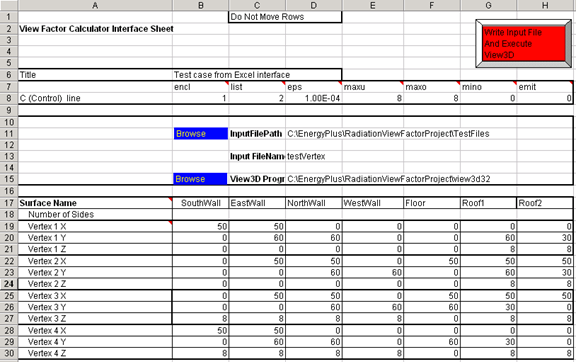
\includegraphics[width=0.9\textwidth, height=0.9\textheight, keepaspectratio=true]{media/image023.png}
\caption{Results in Spreadsheet format \protect \label{fig:results-in-spreadsheet-format}}
\end{figure}

Likewise, a tabular output (usually in HTML format -- which can be read by any web browser) might look like:

\textbf{End Uses}

\begin{longtable}[c]{p{0.85in}p{0.85in}p{0.85in}p{0.85in}p{0.85in}p{0.85in}p{0.85in}}
\toprule 
~ & Electricity (GJ) & Natural Gas (GJ) & Other Fuel (GJ) & Purchaseh Cooling (GJ) & Purchaseh Heating (GJ) & Water (m3) \tabularnewline
\midrule
\endfirsthead

\toprule 
~ & Electricity (GJ) & Natural Gas (GJ) & Other Fuel (GJ) & Purchaseh Cooling (GJ) & Purchaseh Heating (GJ) & Water (m3) \tabularnewline
\midrule
\endhead

Heating & 0.00 & 95.17 & 0.00 & 0.00 & 0.00 & 0.00 \tabularnewline
Cooling & 56.78 & 0.00 & 0.00 & 0.00 & 0.00 & 0.00 \tabularnewline
Interior Lighting & 124.39 & 0.00 & 0.00 & 0.00 & 0.00 & 0.00 \tabularnewline
Exterior Lighting & 0.00 & 0.00 & 0.00 & 0.00 & 0.00 & 0.00 \tabularnewline
Interior Equipment & 28.27 & 0.00 & 0.00 & 0.00 & 0.00 & 0.00 \tabularnewline
Exterior Equipment & 0.00 & 0.00 & 0.00 & 0.00 & 0.00 & 0.00 \tabularnewline
Fans & 73.52 & 0.00 & 0.00 & 0.00 & 0.00 & 0.00 \tabularnewline
Pumps & 0.00 & 0.00 & 0.00 & 0.00 & 0.00 & 0.00 \tabularnewline
Heat Rejection & 0.00 & 0.00 & 0.00 & 0.00 & 0.00 & 0.00 \tabularnewline
Humidification & 0.00 & 0.00 & 0.00 & 0.00 & 0.00 & 0.00 \tabularnewline
Heat Recovery & 0.00 & 0.00 & 0.00 & 0.00 & 0.00 & 0.00 \tabularnewline
Water Systems & 0.08 & 85.39 & 0.00 & 0.00 & 0.00 & 363.07 \tabularnewline
Refrigeration & 0.00 & 0.00 & 0.00 & 0.00 & 0.00 & 0.00 \tabularnewline
Generators & 0.00 & 0.00 & 0.00 & 0.00 & 0.00 & 0.00 \tabularnewline
~ & ~ & ~ & ~ & ~ & ~ & ~ \tabularnewline
Total End Uses & 283.03 & 180.56 & 0.00 & 0.00 & 0.00 & 363.07 \tabularnewline
\bottomrule
\end{longtable}


\chapter{HVAC Diagram}\label{hvac-diagram}


\section{CSVProc}\label{csvproc}

This simple post processing program uses .csv files (such as created by ReadVarsESO) and performs some simple statistics on the contents. This program is described more fully in the Auxiliary Programs document.


\chapter{convertESOMTR}\label{convertesomtr}

This simple post processing utility will convert the raw data ``ESO'' and ``MTR'' files to IP (Inch-Pound) units before later processing into CSV files. EP-Launch has an option to automatically convert to IP units that invokes convertESOMTR, see VIEW - Options - Miscellaneous dialog box. The ReadVarsESO program will take these converted files and make them into normal CSV files but will have IP units. The RunEPlus batch file does not include this option but could be edited to perform the same functions if desired.

Technically speaking, the convertESOMTR program uses the ``convert.txt'' file which contains the conversion factors. It creates files ``ip.eso'' and ``ip.mtr'' as appropriate. The batch examples then renames the old eplusout.eso to eplusout.esoold, old eplusout.mtr to eplusout.mtrold and the ip files to the default eplusout.eso, eplusout.mtr.

The convert.txt file contains the conversion factors using three different commands.

conv,\textless{}si-unit\textgreater{},\textless{}ip-unit\textgreater{},\textless{}multiplier\textgreater{},\textless{}offset\textgreater{}

wild,\textless{}match-string\textgreater{},\textless{}si-unit\textgreater{},\textless{}ip-unit\textgreater{}

vari,\textless{}variable-name-no-units\textgreater{},\textless{}si-unit\textgreater{},\textless{}ip-unit\textgreater{}

If a specific variable needs to be converted, the `vari' line may be used to convert the units on that specific variable only. To convert a class of variables that contains a specific string of characters in the names of the variables, the `wild' line may be used. The `conv' lines are the lines that actually create the conversion factors. If no `vari' or `wild' match a variable, then it is converted used the first `conv' line that matches. The default convert.txt file contains some conversions for Inch-Pound units but any set of units may be used by editing the convert.txt file. Note that the convert.txt file uses the standard EnergyPlus comment character (!).

A snippet of the convert.txt file:

\begin{lstlisting}
! Power
!------------------------------
!    (1 kW / 1000 W)
conv,W,kW,0.001,0
!    (1 Btuh/ 0.2928751 W) * (1 kBtuh/1000 Btuh)
conv,W,kBtuh,3.41442E-03,0
\end{lstlisting}


\section{DataFiles}\label{datafiles}

Some example files are installed during installation (Sample Files option). Each sample input file should contain comments about its purpose at the start of the file. Other example files are made available from the website (\url{http://www.energyplus.gov/}).


\section{Library Files}\label{library-files}

Library files for EnergyPlus are embodied in the DataSets and MacroDataSets folders. DataSets are IDF excerpts -- you must cut and paste from them in order to use them. Items in MacroDataSets can be used in conjunction with the EPMacro preprocessor program. All files are in the necessary form for processing with EnergyPlus.

The files in the DataSets and MacroDataSets folders are described in more detail in the ``\href{file:///E:/Docs4PDFs/OutputDetailsAndExamples.pdf}{Output Details and Examples}'' document.


\chapter{Energy Meters}\label{energy-meters}


\section{Standard Energy Meters}\label{standard-energy-meters}

Meters provide one way for EnergyPlus to report energy use in a form that is pallatable to the users. The primary implemented method for output gives very fine detail (down to the variable level) for results from EnergyPlus. However, to get the required energy use, there may be several variables that need to be polled and accumulated. The meter implementation for EnergyPlus accomplishes this reporting.

\begin{figure}[hbtp] % fig 24
\centering
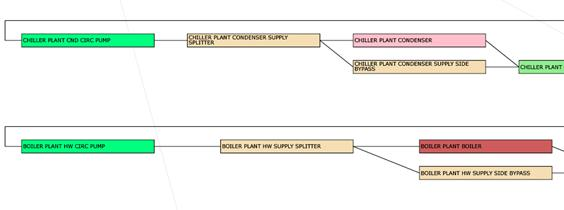
\includegraphics[width=0.9\textwidth, height=0.9\textheight, keepaspectratio=true]{media/image024.jpg}
\caption{Illustration of Energy Metering \protect \label{fig:illustration-of-energy-metering}}
\end{figure}

Meters can be used to typify energy use by type and by component. The diagrams and tables illustrate how the meters have been incorporated into EnergyPlus.

As shown in the figure above, energy use for the facility is grouped according to fuel type (see Table~\ref{table:table-of-metered-fuel-types}. Table of Metered Fuel Types), by meter type (see Table~\ref{table:overall-meter-types}. Overall Meter Types) and by end use category type (see Table~\ref{table:end-use-category-types}. End Use Category Types).

% table 7
\begin{longtable}[c]{@{}l@{}}
\caption{Overall Meter Types \label{table:overall-meter-types}} \tabularnewline
\toprule 
Meters \tabularnewline
\midrule
\endfirsthead

\caption[]{Overall Meter Types} \tabularnewline
\toprule 
Meters \tabularnewline
\midrule
\endhead

Facility \tabularnewline
Building \tabularnewline
Zone \tabularnewline
System \tabularnewline
Plant \tabularnewline
\bottomrule
\end{longtable}

Both the fuel types and enduse types are set within the program by the developers. Current Fuel types are shown in the table below. There is also a special category called ``EnergyTranser''.

% table 8
\begin{longtable}[c]{@{}l@{}}
\caption{Table of Metered Fuel Types \label{table:table-of-metered-fuel-types}} \tabularnewline
\toprule 
Utility/Fuel Types \tabularnewline
\midrule
\endfirsthead

\caption[]{Table of Metered Fuel Types} \tabularnewline
\toprule 
Utility/Fuel Types \tabularnewline
\midrule
\endhead

Electricity \tabularnewline
Gas \tabularnewline
Gasoline \tabularnewline
Diesel \tabularnewline
Coal \tabularnewline
FuelOil\#1 \tabularnewline
FuelOil\#2 \tabularnewline
Propane \tabularnewline
Water \tabularnewline
Steam \tabularnewline
DistrictCooling \tabularnewline
DistrictHeating \tabularnewline
\bottomrule
\end{longtable}

\begin{longtable}[c]{@{}l@{}}
\toprule 
AdditionalTypes \tabularnewline
\midrule
\endfirsthead

\toprule 
AdditionalTypes \tabularnewline
\midrule
\endhead

HeatingCoils \tabularnewline
CoolingCoils \tabularnewline
Chillers \tabularnewline
Boilers \tabularnewline
Baseboard \tabularnewline
HeatRecoveryForCooling \tabularnewline
HeatRecoveryForHeating \tabularnewline
\bottomrule
\end{longtable}

The end use types are shown in the following table:

% table 9
\begin{longtable}[c]{@{}l@{}}
\caption{End Use Category Types \label{table:end-use-category-types}} \tabularnewline
\toprule 
End Use Types \tabularnewline
\midrule
\endfirsthead

\caption[]{End Use Category Types} \tabularnewline
\toprule 
End Use Types \tabularnewline
\midrule
\endhead

InteriorLights \tabularnewline
ExteriorLights \tabularnewline
InteriorEquipment \tabularnewline
ExteriorEquipment \tabularnewline
Fans \tabularnewline
Pumps \tabularnewline
Heating \tabularnewline
Cooling \tabularnewline
HeatRejection \tabularnewline
Humidifier \tabularnewline
HeatRecovery \tabularnewline
DHW \tabularnewline
Cogeneration \tabularnewline
Refrigeration \tabularnewline
Miscellaneous \tabularnewline
\bottomrule
\end{longtable}

Additional End Use Types Only Used for EnergyTransfer:

\begin{longtable}[c]{@{}l@{}}
\toprule 
AdditionalTypes \tabularnewline
\midrule
\endfirsthead

\toprule 
AdditionalTypes \tabularnewline
\midrule
\endhead

HeatingCoils \tabularnewline
CoolingCoils \tabularnewline
Chillers \tabularnewline
Boilers \tabularnewline
Baseboard \tabularnewline
HeatRecoveryForCooling \tabularnewline
HeatRecoveryForHeating \tabularnewline
\bottomrule
\end{longtable}


\section{Custom Meters}\label{custom-meters}

You can also define your own ``custom meters'' from variable names that are summed during the simulation.~ You assign the proper fuel type during the definition (review Input Output Reference, objects: \textbf{Meter:Custom} and \textbf{Meter:CustomDecrement}) for further requirements.


\section{Standard EnergyPlus Units}\label{standard-energyplus-units}

EnergyPlus expects information in a single unit system (SI). This requires interface developers to convert user inputs from those preferred by architects and engineers into the standard metric units of EnergyPlus. EnergyPlus will not perform any units conversions and will not have any unit conversion routines.

ASCII with no spaces is used for abbreviations. Note that exponents appear without any indication of exponentiation: i.e., kg/m3 not kg/m\^{}3 or kg/m**3. Also note the use of dashes. We have W/m2-K not W/m2*K or W/(m2*K).

At the end we note the ``problem'' variables -- the inputs that have non-standard units. Inputs using these units will have to be changed and the code checked to see how the quantities are used internally.

\begin{longtable}[c]{p{1.59in}p{2.9in}p{1.5in}}
\caption{Standard EnergyPlus Units \label{table:standard-energyplus-units}} \tabularnewline
\toprule 
Quantity & unit & abbreviation \tabularnewline
\midrule
\endfirsthead

\caption[]{Standard EnergyPlus Units} \tabularnewline
\toprule 
Quantity & unit & abbreviation \tabularnewline
\midrule
\endhead

angular degrees & degree & deg \tabularnewline
Length & meter & m \tabularnewline
Area & square meter & m2 \tabularnewline
Volume & cubic meter & m3 \tabularnewline
Time & seconds & s \tabularnewline
Frequency & Hertz & Hz \tabularnewline
Temperature & Celsius & C \tabularnewline
absolute temperature & Kelvin & K \tabularnewline
temperature difference & Kelvin & deltaC \tabularnewline
speed & meters per second & m/s \tabularnewline
energy (or work) & Joules & J \tabularnewline
power & Watts & W \tabularnewline
mass & kilograms & kg \tabularnewline
force & Newton & N \tabularnewline
mass flow & kilograms per second & kg/s \tabularnewline
volume flow & cubic meters per second & m3/s \tabularnewline
pressure & Pascals & Pa \tabularnewline
pressure difference & Pascals & Pa \tabularnewline
specific enthalpy & Joules per kilogram & J/kg \tabularnewline
density & kilograms per cubic meter & kg/m3 \tabularnewline
heat flux & watts per square meter & W/m2 \tabularnewline
specific heat & ------- & J/kg-K \tabularnewline
conductivity & ------- & W/m-K \tabularnewline
diffusivity & ------- & m2/s \tabularnewline
heat transfer coefficient & ------- & W/m2-K \tabularnewline
R-value & ------- & m2-K/W \tabularnewline
heating or cooling capacity & Watts & W \tabularnewline
electric potential & volts & V \tabularnewline
electric current & Amperes & A \tabularnewline
illuminace & lux & lx \tabularnewline
luminous flux & lumen & lm \tabularnewline
luminous intensity & candelas & cd \tabularnewline
luminance & candelas per square meter & cd/m2 \tabularnewline
vapor diffusivity & meters squared per second & m2/s \tabularnewline
viscosity & ------- & kg/m-s \tabularnewline
dynamic Viscosity & ------- & N-s/m2 \tabularnewline
thermal gradient coeff for moisture capacity & ------- & kg/kg-K \tabularnewline
isothermal moisture capacity & ------- & m3/kg \tabularnewline
\bottomrule
\end{longtable}


\end{document}


\section{Comparing EnergyPlus to Other Programs}\label{comparing-energyplus-to-other-programs}

A paper comparing and contrasting Energy Simulation Programs can be found here:

\url{http://www.eere.energy.gov/buildings/tools_directory/pdfs/contrasting_the_capabilities_of_building_energy_performance_simulation_programs_v1.0.pdf}

As this paper was published in 2005, it is out of date (at least with current EnergyPlus capabilities).

The feature highlights from EnergyPlus releases can be seen here:

\url{http://apps1.eere.energy.gov/buildings/energyplus/pdfs/featurehighlights.pdf}

In addition you can see how EnergyPlus compares to other programs (which have submitted their models) in our testing reports:

\url{http://apps1.eere.energy.gov/buildings/energyplus/testing.cfm}


\section{DataSets}\label{datasets}

Akin to the libraries of other programs, EnergyPlus uses data sets.~ Data sets are similar to libraries but many items are contained in a single file (usually input file format or sometimes macro format).~ Developers are encouraged, as appropriate, to submit data sets along with new features.~ Some of the existing data sets include:

\begin{itemize}
\item
  Materials properties
\item
  Construction elements (layers of materials)
\item
  Composite construction definitions (equivalent constructions for complex elements)
\item
  Solar Collector parameters
\item
  Economic Tariffs
\item
  Design Day definitions
\item
  Location definitions
\item
  Standard report definitions
\end{itemize}


\section{Datasets aka Libraries}\label{datasets-aka-libraries}

EnergyPlus uses the term DataSets for what many would call libraries. These files are included, for the most part, in the instalation package but may be available from other sites (such as the helpdesk or Yahoo Groups).

There are two flavors of DataSets: \textbf{simple} and \textbf{Macro}. Some sets have files in both camps (for example, Solar Collectors). Both flavors contain IDF objects ready to be put into EnergyPlus input files. With the simple datasets, you may need to use a text editor or the IDF Editor to search the file for the one you want to use.~ With the macro datsets and a simply structured imf (input macro file), you can name the item you want to include. (The macro program is described in the \href{file:///E:/Docs4PDFs/AuxiliaryPrograms.pdf}{Auxiliary Programs document}).

Primary documentation for each dataset is found in the \href{file:///E:/Docs4PDFs/OutputDetailsAndExamples.pdf}{Output Details and Examples document}. Highlights of some datasets are given here.


\section{Locations-DesignDays}\label{locations-designdays}

This file (Locations-DesignDays.xls) can be found in the MacroDataSets folder. While not strictly a macro file, it leads one to be able to download the ASHRAE design day definitions from the EnergyPlus website. The spreadsheet format contains a sheet for each of the WMO regions as well as the California Climate Zones, specifically sheets included are:

\begin{itemize}
\item
  Readme -- an upfront readme page
\item
  WMO1 Africa
\item
  WMO2 Asia
\item
  WMO3 South America
\item
  WMO4 North \& Central America
\item
  CZ Files -- California Climate Zones
\item
  WMO5 Southwest Pacific
\item
  WMO6 Europe
\item
  WMO7 Antarctica
\end{itemize}

Each WMO (World Meteorological Organization) page contains the countries represented, specific cities that have design conditions data from ASHRAE, a link to the full imf file with location, daylighting saving and design day definitions as well as a link to that region's weather page on the EnergyPlus website. Pressing the links here will allow you to download the files.


\chapter{Design Day / Weather Data}\label{design-day-weather-data}


\section{Design Day Creation}\label{design-day-creation}

\emph{How do I create the profile used in the SizingPeriod:DesignDay object?}

Typically, the EnergyPlus Development Team uses the data from the most recent ASHRAE Handbook of Fundamentals to create a set of design day profiles that can be used. Description of ASHRAE's data is contained in Chapter 14 of the 2009 Handbook of Fundamentals. Table~\ref{table:multistory-vs-multistory-2-and-multistory-3} shows the kind of data that is embodied in the design day definitions shown earlier (ref. Locations-DesignDays).

Design Days (aka Design Conditions) are very important for use in HVAC Sizing calculations -- refer to the ASHRAE Handbook of Fundamentals for further information.

From this, you can determine if you should use one of these profiles and modify it or determine how to create your own profile.

The Weather Converter program accesses this file when it processes (even for statistics) a weather file. Design Day definitions are also included with the zips on the EnergyPlus weather data site. For locations that don't have ASHRAE design conditions, the Weather Converter uses the data within the weather file to generate pseudo conditions in the statistics file.


\section{EPW Weather Files}\label{epw-weather-files}

The WeatherConverter converts from other source formats to EPW and EnergyPlus CSV formats. The WeatherConverter also produces a statistics file that provides a quick synopsis of the converted data and is used by the tabular reports (ref: Climatic Data Summary report). For Ecotect users, the Weather Converter can also save as .wea format. We do not support conversion of EPWs to other formats, including to TMY2. The Weather Converter is described in detail in the \href{file:///E:/Docs4PDFs/AuxiliaryPrograms.pdf}{Auxiliary Programs document}.


\section{Meteonorm Weather Files}\label{meteonorm-weather-files}

For locations that aren't on the regular EnergyPlus weather site (\url{http://apps1.eere.energy.gov/buildings/energyplus/cfm/weather_data.cfm}), the team has created weather data using the Meteonorm™ software. Meteonorm extrapolates hourly data from statistical data for a location. Where statistical data aren't available, Meteonorm interpolates from other nearby sites. Generally, a statistical approach is a last resort---weather files generated from statistics will not demonstrate the normal hour-to-hour and day-to-day variability seen in measured data. Each .ZIP includes a .STAT (EnergyPlus weather data statistics), .EPW (EnergyPlus weather file), and .INFO (Information about the source data and limitations from Meteonorm).

In all cases, review the .STAT file for the location before using any of these files to ensure that it represents the climate of the locations as you understand it. In many cases, a nearby location with measured data may be more appropriate than one derived from statistics. These files, once created, are published on the EnergyPlus Yahoo Group site.

As always, if you know of sources of weather data that we might be able to share with the EnergyPlus community, please contact us.


\section{Weather Data for Simulations}\label{weather-data-for-simulations}

Weather data can be used for various purposes by simulation program such as EnergyPlus. For some purposes, such as validating a model to actual energy use, you may wish to match the weather data to the simulation period. However, for most purposes, you will wish to have a more typical weather data profile. Information on selecting weather data is described in this paper:

Drury B. Crawley. 1998. ``Which Weather Data Should You Use for Energy Simulations of Commercial Buildings?'' in ASHRAE Transactions, pp.~498-515, Vol. 104, Pt. 2. Atlanta: ASHRAE. (PDF 197 KB)

PDF: \url{http://energyplus.gov/pdfs/bibliography/whichweatherdatashouldyouuseforenergysimulations.pdf}


\section{Weather File Sources}\label{weather-file-sources}

The description of sources for the EnergyPlus weather data that is on the website are available here: \url{http://apps1.eere.energy.gov/buildings/energyplus/weatherdata_sources.cfm}


\section{Measuring Solar Data}\label{measuring-solar-data}

\emph{Can the following weather file metrics be directly measured by some inexpensive devices?}

Extraterrestrial Horizontal Radiation \{Wh/m2\} Extraterrestrial Direct Normal Radiation \{Wh/m2\} Horizontal Infrared Radiation Intensity from Sky \{Wh/m2\} Global Horizontal Radiation \{Wh/m2\} Direct Normal Radiation \{Wh/m2\} Diffuse Horizontal Radiation \{Wh/m2\} Global Horizontal Illuminance \{lux\} Direct Normal Illuminance \{lux\} Diffuse Horizontal Illuminance \{lux\}*

You can't measure extraterrestrial unless you're in outer space, but then it's assumed to be constant anyway. For the various radiation and illuminance values, they can measured by various instrumentation ranging from the very cheap to the very expensive. Properly, radiation needs to be measured with a pyranometer (Eppley), which is pricy, but I'm also seen people use simpler apparatus (Lycors) that are really photometers. Direct beam is generally not measured, but derived by subtracting the diffuse from the global. Diffuse is measured by adding a shadow band over a pyranometer to block out the direct beam. Pyranometers measure heat, photometers measure light. All the illuminance on the weather files are derived from the radiation and sky conditions.

Do not forget that the quantities you list are the inputs to the models that are used to derive the variables you really need in practice: irradiance and illuminance on the facets of the building (windows especially). These facets are usually NOT horizontal. Measuring all the components for all tilts and azimuths can be a costly proposition, and that's why it is rarely done (hence the need for models), but that's what should be done in serious experiments to remove the (large) uncertainties in modeled radiation.

Illuminance is measured with photometers (from, e.g., Licor), which resemble silicon-based pyranometers. Both are less costly than thermopile radiometers, which are normally the best in terms of accuracy. Measurements obtained with silicon-based pyranometers need various corrections to account for their limited spectral range. No correction is needed for photometers, though. So you have this issue of accuracy vs cost to consider.

Direct irradiance is measured with a pyrheliometer, which tracks the sun and is therefore costly, but also the most accurate of all radiometers. Obtaining direct irradiance by subtracting diffuse from global is convenient, but not accurate, as shown in recent publications.


\chapter{Input}\label{input}


\section{Creating Files for EnergyPlus}\label{creating-files-for-energyplus}

The install package includes the IDF Editor (Windows platform) for creating EnergyPlus Input Files (aka IDFs). Likewise, text editors such as NotePad or WordPad can be used to create flat ASCII files for use with EnergyPlus.

\subsection{dxf or dwg CAD Files}\label{dxf-or-dwg-cad-files}

\emph{How can I convert dxf or dwg CAD files to EnergyPlus?}

Several EnergyPlus interfaces, including DesignBuilder and OpenStudio (plug in for Google SketchUp), allow you to import the dxf drawings and trace over them to create EnergyPlus geometry. If you have the full AutoCAD 3-D dwg model (more than just dxf), then you might be able to export to EnergyPlus using one of the available utilities that work with AutoCAD, but only if the model was created in the correct way to support these tools. As of February 2009, Green Building Studio and EnergyPlugged (a plug in to AutoCAD) support export to EnergyPlus.

For more information about current tools which support EnergyPlus, see \url{http://www.energyplus.gov/interfaces_tools.cfm}.

\subsection{OpenStudio for Google Sketchup}\label{openstudio-for-google-sketchup}

\href{http://apps1.eere.energy.gov/buildings/energyplus/openstudio.cfm}{OpenStudio} is a free plugin for the Google SketchUp 3D drawing program. The plugin makes it easy to create and edit the building geometry in your EnergyPlus input files. The plugin also allows you to launch EnergyPlus simulations and view the results without leaving SketchUp.

\subsection{EnergyPlus Example File Generator}\label{energyplus-example-file-generator}

A Web-based service is available that creates and runs EnergyPlus input files for simple models of commercial buildings. The input files (and annual results summary files) are sent to your e-mail address as attachments. You can access the service and customize the characteristics of the building you want to model on the \href{http://apps1.eere.energy.gov/buildings/energyplus/cfm/inputs/}{EnergyPlus Example File Generator Application} (pop-ups must be enabled). Learn more by viewing the \href{http://apps1.eere.energy.gov/buildings/energyplus/cfm/inputs/help.cfm}{EnergyPlus Building Data Input Forms Help} File.


\section{Converting Older Version EnergyPlus Files}\label{converting-older-version-energyplus-files}

\emph{Can I convert an older file to a newer version of EnergyPlus?}

If the older version is from the previous release, then yes. Use the pull-down File menu and select Transition. This will update the older file to the newer version.

If the older version is older than the previous release, then you must use the multiple transition program. You can download the transition programs from this site.

(That is \url{http://energyplus.helpserve.com} and go to the ``downloads'' area).

The Multiple Transition folder is set up on the EnergyPlus install.

Unzip the file into the MultipleTransition folder and use the IDF Converter GUI program to transition your older files. The IDF converter can also save the transitioned file for each intermediate version, if desired.


\section{Using Macros and Editing Inputs in IDF Editor}\label{using-macros-and-editing-inputs-in-idf-editor}

\emph{How can I use macros, and continue to edit my input in IDF editor?}

\emph{(Using or ignoring macros in the IDF editor is a potential Enhancement List item.)}

1)~~~Separate files into ``IDF editable'' and ``macro'' (actually, the AbsorptionChiller\_Macro.imf example file shows a little of this but it doesn't really use macros). For the pieces you think you'd like to manipulate in the IDF editor, call them with extension IDF. For the others, they would be IMF and the master file would be IMF with ``includes'' of your IDF pieces.

2)~~~Use the expanded IDF (extension epmidf) file for your IDF editor changes and then run it from there.


\section{Getting data from WINDOW program}\label{getting-data-from-window-program}

The WINDOW program is published from LBNL at \url{http://windows.lbl.gov/software}. More specifics on the program and its details are shown in the Input Output Reference under ``Importing Windows from WINDOW program'' topic.

\subsection{EnergyPlus IDF Excerpt Data}\label{energyplus-idf-excerpt-data}

The preferred method of using WINDOW data in EnergyPlus is to excerpt or ``report'' a specific Window from the Window library screen (see below):

\begin{figure}[hbtp] % fig 1
\centering
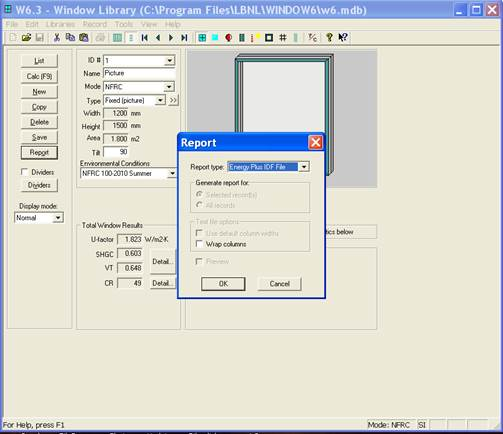
\includegraphics[width=0.9\textwidth, height=0.9\textheight, keepaspectratio=true]{media/image001.jpg}
\caption{WINDOW screen for exporting IDF Window specifications \protect \label{fig:window-screen-for-exporting-idf-window}}
\end{figure}

The file can then be saved at a location of your choice and added into your overall simulation IDF file.

\subsection{WINDOW Data File}\label{window-data-file}

The other ``older'' option for creating data for EnergyPlus is to use the ``EnergyPlus'' option above and create a WindowDataFile. The general format of this data is described in the following paragraphs and must use the Construction:WindowDataFile object and an external file to be used in EnergyPlus. While this is a convenient small file (that can contain multiple windows), there is no way to import this file back into WINDOW and obtain the above, more preferred method.

Please note that there is a bug in WINDOW 5 that causes two of the lines in the EnergyPlus data file to be joined. This bug is fixed in versions of Window 5.02 (and above). To be sure, you can check the data file for a line that looks like:

GLAZING SYSTEM OPTICAL DATAAngle~~~~ 0~~~ 10~~~ 20~~~ 30~~~ 40~~~ 50~~~ 60~~~ 70~~~ 80~~~ 90 Hemis

The fixed version of the program will not show the above line; rather, there will be two lines such as shown below. If you have the above condition, with an editor you would break this into two lines:

GLAZING SYSTEM OPTICAL DATA

Angle~~~~ 0~~~ 10~~~ 20~~~ 30~~~ 40~~~ 50~~~ 60~~~ 70~~~ 80~~~ 90 Hemis

In EnergyPlus, the Window data file is searched for each ``Construction:WindowDataFile'' object in the EnergyPlus input. This object has a very simple form:

Construction:WindowDataFile,

ConstructionName,

FileName; ! Default is Window5DataFile.dat in the ``run'' folder.

If there is a window called ConstructionName on the Window data file, the data for that window is read from the file and the following EnergyPlus objects and their names are created. The ``W5'' prefixed to these names indicates that the object originated in the Window5 data file.

\begin{itemize}
\item
  \textbf{WindowMaterial:Glazing} for each of the glass layers. They will be named \textbf{W5:ConstructionName:GLASS1}, \textbf{W5:ConstructionName:GLASS2} , etc.
\item
  \textbf{WindowMaterial:Gas} or \textbf{WindowMaterial:GasMixture} for each of the gap layers. They will be named \textbf{W5:ConstructionName:GAP1}, \textbf{W5:ConstructionName:GAP2} , etc.
\item
  \textbf{WindowProperty:FrameAndDivider} (if the window on the Window5 data file has a frame and/or divider). It will be named \textbf{W5:ConstructionName}. This WindowProperty:FrameAndDivider will be assigned to any window on the input file that has a construction called ``ConstructionName'' \emph{even if that window has~ referenced another WindowProperty:FrameAndDivider (i.e., if WindowProperty:FrameAndDivider Name for that window is specified).} In this case a warning will result.
\end{itemize}

Note that:

An entry on the WINDOW data file usually has just one glazing system. It is also possible to have an entry with two glazing systems separated by a horizontal or vertical mullion. In this case, the two glazing systems can have different dimensions and different properties. For example, one of the two glazing systems could be single glazed and the other could be double glazed. An example~ of the two glazing system case is given in the sample WINDOW data file shown below (although in this case the properties of the two glazing systems are the same).

EnergyPlus handles the ``one glazing system'' and ``two glazing systems'' cases differently. If there is one glazing system, the glazing system height and width from the Window5 data file are not used. Instead, the window dimensions are obtained from the window vertices that have been specified on the IDF file. However, a warning message will result if the height or width calculated from the window's vertex inputs differs from the corresponding Window5 data file values by more than 10\%. This warning is given since the effective frame and edge-of-glass conductances on the WINDOW data file can depend on the window dimensions if the frame is non-uniform, i.e., consists of sections with different values of width, projection, or thermal properties.

If the WINDOW data file entry has two glazing systems, System1 and System2, the following happens, as shown in the figure below. Assume that the original window is called WinOriginal. System1 is assigned to WinOriginal. Then EnergyPlus automatically creates a second window, called WinOriginal:2, and assigns System2 to it. The dimensions of WinOriginal are ignored; the dimensions of System1 on the data file are assigned to it, but the position of the lower left-hand vertex of WinOriginal is retained. The dimensions of System2 on the data file are assigned to WinOriginal:2. The lower left-hand vertex of WinOriginal:2 is determined from the mullion orientation and width.

\textbf{Note: WinOriginal would have been the IDF window definition -- it's dimensions will be overridden by the systems dimensions from the Window data file. Two windows will be made and called WinOriginal and WinOriginal:2.}

\begin{figure}[hbtp] % fig 2
\centering
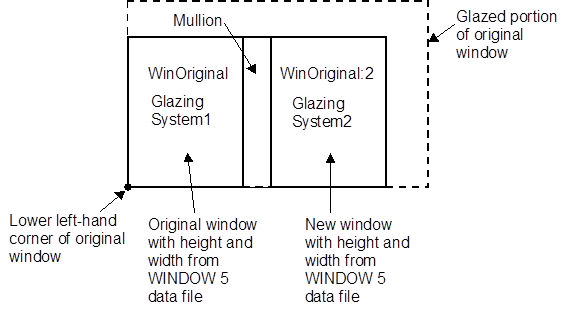
\includegraphics[width=0.9\textwidth, height=0.9\textheight, keepaspectratio=true]{media/image002.png}
\caption{Window Glazing system with dual glazing constructions \protect \label{fig:window-glazing-system-with-dual-glazing}}
\end{figure}

The Window Data File contains no information on shading devices. See ``Specify the Material Name of the Shading Device'' under WindowProperty:ShadingControl for a method to attach a shading layer to windows read in from this file.

Following is an example WINDOW data file for a slider window with two identical double low-E glazing systems separated by a horizontal mullion. Each system has a frame and divider. Note that all dimensions, such as glazing height and width, are in millimeters; when EnergyPlus reads the file these are converted to meters. Following the data file example is a description of the contents of the file. That data used by EnergyPlus is shown in bold.

Window5 Data File for EnergyPlus

\textless{}WINDOW program version\textgreater{}

Date~~~~~~~~~~~~ : Tue Nov 13 17:07:40 2001

Window name~~~~~ : \textbf{DoubleLowE}

Description~~~~~ : Horizontal Slider, AA

\# Glazing Systems: \textbf{2}

GLAZING SYSTEM DATA: Height Width nPanes Uval-center SC-center SHGC-center Tvis-center

~System1~~~~~~~~ :~~ 1032~~ 669~~~~~ 2~~~~~ 1.660~~~~~ 0.538~~~~~ 0.467~~~~~~ 0.696

~System2~~~~~~~~ :~~ 1033~~ 669~~~~~ 2~~~~~ 1.660~~~~~ 0.538~~ ~~~0.467~~~~~~ 0.696

FRAME/MULLION DATA: Width OutsideProj InsideProj Cond EdgeCondRatio SolAbs VisAbs Emiss~ Orient'n (mull)

~~~ L Sill~~~~~~ :~~ 97.3~~~~ 25.4~~~~~~ 25.4~~ 500.000~~~ 1.467~~~~ 0.500~ 0.500~ 0.90

~~~ R Sill~~~~~~ :~~ 97.3~~~~ 25.4~~~~~~ 25.4~~ 500.000~~~ 1.467~~~~ 0.500~ 0.500~ 0.90

~~~ L Head~~~~~~ :~~ 70.2~~~~ 25.4~~~~~~ 25.4~~ 18.822~~~~ 1.490~~~~ 0.500~ 0.500~ 0.90

~~~ R Head~~~~~~ :~~ 70.2~~~~ 25.4~~~~~~ 25.4~~ 18.822~~~~ 1.490~~~~ 0.500~ 0.500~ 0.90

~~~ Top L Jamb~~ :~~ 54.3~~~~ 25.4~~~~~~ 25.4~~ 31.141~~~~ 1.503~~~~ 0.500~ 0.500~ 0.90

~~~ Bot L Jamb~~ :~~ 54.3~~~~ 25.4~~~~~~ 25.4~~ 500.000~~~ 1.494~~~~ 0.500~ 0.500~ 0.90

~~~ Top R Jamb~~ :~~ 70.2~~~~ 25.4~~~~~~ 25.4~~ 500.000~~~ 1.518~~~~ 0.500~ 0.500~ 0.90

~~~ Bot R Jamb~~ :~~ 97.6 ~~~~25.4~~~~~~ 25.4~~ 264.673~~~ 1.547~~~~ 0.500~ 0.500~ 0.90

~~~ Mullion~~~~~ :~~ 53.5~~~~ 25.4~~~~~~ 25.4~~ 500.000~~~ 1.361~~~~ 0.500~ 0.500~ 0.90 \textbf{Horizontal}

~~~ Average frame:~~ \textbf{75.5~~~~ 25.4~~~~~~ 25.4~~ 326.149~~~ 1.464~~~~ 0.500~ 0.500~ 0.90}

DIVIDER DATA~~~~ : Width OutsideProj InsideProj Cond EdgeCondRatio SolAbs VisAbs Emiss Type~~~~~~~~~~~ \#Hor \#Vert

~System1~~~~~~~~ :~ \textbf{25.4~~~ 25.4~~~~~~ 25.4~~~ 3.068~~~~~ 1.191~~~~ 0.500~ 0.500 0.900 DividedLite~~~~~~ 2~~~ 3}

~System2~~~~~~~~ :~ \textbf{25.4~~~ 25.4~~~~ ~~25.4~~~ 3.068~~~~~ 1.191~~~~ 0.500~ 0.500 0.900 DividedLite~~~~~~ 2~~~ 3}

GLASS DATA~~~~~~ : Layer\#~ Thickness~ Cond Tsol Rfsol Rbsol Tvis Rfvis Rbvis~ Tir~ EmissF~ EmissB~ SpectralDataFile

~System1~~~~~~~~ :~~ 1~~~~~ \textbf{3.00~~~~ 0.900} 0.50~ 0.33~ 0.39 0.78~ 0.16~ 0.13 \textbf{0.00~~ 0.16~~~ 0.13}~~ CMFTIR\_3.AFG

~~~~~~~~~~~~~~~~~~~~ 2~~~~~ \textbf{6.00~~~~ 0.900} 0.77~ 0.07~ 0.07 0.88~ 0.08~ 0.08 \textbf{0.00~~ 0.84~~~ 0.84}~~ CLEAR\_6.DAT

~System2~~~~~~~~ :~~ 1~~~~~ \textbf{3.00~~~~ 0.900} 0.50~ 0.33~ 0.39 0.78~ 0.16~ 0.13 \textbf{0.00~~ 0.16~~~ 0.13}~~ CMFTIR\_3.AFG

~~~~~~~~~~~~~~~~~~~~ 2~~~~~ \textbf{6.00~~~~ 0.900} 0.77~ 0.07~ 0.07 0.88~ 0.08~ 0.08 \textbf{0.00~~ 0.84~~~ 0.84}~~ CLEAR\_6.DAT

GAP DATA~~~~~~~~ : Gap\# Thick nGasses

~System1~~~~~~~~ :~~ 1~ \textbf{12.70~~~ 1}

~System2~~~~~~~~ :~~ 1~ \textbf{12.70~~~ 1}

GAS DATA~~~~~~~~ : GasName Fraction MolWeight ACond~~ BCond~ CCond AVisc~~ BVisc~~ CVisc ASpHeat~ BSpHeat CSpHeat

~System1 Gap1~~~ : Air~~~~ \textbf{1.0000~~ 28.97~~~ 0.002873 7.76e-5 0.0 3.723e-6 4.94e-8 0.0~~ 1002.737 0.012324 0.0}

~System2 Gap1~~~ : Air~~~~ \textbf{1.0000~~ 28.97~~~ 0.002873 7.76e-5 0.0 3.723e-6 4.94e-8 0.0~~ 1002.737 0.012324 0.0}

GLAZING SYSTEM OPTICAL DATA

Angle~~~~ 0~~~ 10~~~ 20~~~ 30~~~ 40~~~ 50~~~ 60~~~ 70~~~ 80~~~ 90 Hemis

System1

Tsol~ \textbf{0.408 0.410 0.404 0.395 0.383 0.362 0.316 0.230 0.106 0.000 0.338}

Abs1~ \textbf{0.177 0.180 0.188 0.193 0.195 0.201 0.218 0.239 0.210 0.001 0.201}

Abs2~ \textbf{0.060 0.060 0.061 0.061 0.063 0.063 0.061 0.053 0.038 0.000 0.059}

Rfsol \textbf{0.355 0.350 0.348 0.350 0.359 0.374 0.405 0.478 0.646 0.999 0.392}

Rbsol \textbf{0.289 0.285 0.283 0.282 0.285 0.296 0.328 0.411 0.594 1.000 0.322}

Tvis~ \textbf{0.696 0.700 0.690 0.677 0.660 0.625 0.548 0.399 0.187 0.000 0.581}

Rfvis \textbf{0.207 0.201 0.198 0.201 0.212 0.234 0.278 0.374 0.582 0.999 0.260}

Rbvis \textbf{0.180 0.174 0.173 0.176 0.189 0.215 0.271 0.401 0.648 1.000 0.251}

System2

Tsol~ \textbf{0.408 0.410 0.404 0.395 0.383 0.362 0.316 0.230 0.106 0.000 0.338}

Abs1~ \textbf{0.177 0.180 0.188 0.193 0.195 0.201 0.218 0.239 0.210 0.001 0.201}

Abs2~ \textbf{0.060 0.060 0.061 0.061 0.063 0.063 0.061 0.053 0.038 0.000 0.059}

Rfsol \textbf{0.355 0.350 0.348 0.350 0.359 0.374 0.405 0.478 0.646 0.999 0.392}

Rbsol \textbf{0.289 0.285 0.283 0.282 0.285 0.296 0.328 0.411 0.594 1.000 0.322}

Tvis~ \textbf{0.696 0.700 0.690 0.677 0.660 0.625 0.548 0.399 0.187 0.000 0.581}

Rfvis \textbf{0.207 0.201 0.198 0.201 0.212 0.234 0.278 0.374 0.582 0.999 0.260}

Rbvis \textbf{0.180 0.174 0.173 0.176 0.189 0.215 0.271 0.401 0.648 1.000 0.251}

\textbf{Description of Contents of WINDOW Data File}

(Quantities used in EnergyPlus are in bold; others are informative only)

Second line = version of WINDOW used to create the data file

\emph{Date} = date the data file was created

\textbf{\emph{Window name}} = name of this window; chosen by WINDOW5 user; EnergyPlus user enters the same name in EnergyPlus as name of a ``Construction from Window5 Data File'' object. EnergyPlus will search the Window5 data file for an entry of this name.

\emph{Description} = One-line description of the window; this is treated as a comment.

\textbf{\emph{\# Glazing Systems}}: 1 or 2; value is usually 1 but can be 2 if window has a horizontal or vertical mullion that separates the window into two glazing systems that may or may not be different.

GLAZING SYSTEM DATA

\emph{System1, System2}: separate characteristics given if window has a mullion.

\textbf{\emph{Height}}, *\textbf{\emph{width}} = height and width of glazed portion (i.e., excluding frame; and, if mullion present, excluding mullion).

\textbf{\emph{nPanes}}~~~~ = number of glass layers

\emph{Uval-center} = center-of-glass U-value (including air films) under standard winter conditions*~ (W/m2)

\emph{SC-center}~~ = center-of-glass shading coefficient under standard summer conditions*.

\emph{SHCG-center} = center-of-glass solar heat gain coefficient under standard summer conditions*.

\emph{Tvis-center} = center-of-glass visible transmittance at normal incidence

FRAME/MULLION DATA

\emph{L,R Sill}~~ = left, right sill of frame

\emph{L,R Head}~~ = left, right header of frame

\emph{Top L, Bot L jamb} = top-left, bottom-left jamb of frame

\emph{Bot L, Bot R jamb} = bottom-left, bottom-right jamb of frame

\textbf{\emph{Average frame}} = average characteristics of frame for use in EnergyPlus calculation. If mullion is present, original window is divided into two separate windows with the same average frame (with the mullion being split lengthwise and included in the average frame).

\textbf{\emph{Width}}~~~~ = width (m)

\textbf{\emph{OutsideProj}} = amount of projection from outside glass (m)

\textbf{\emph{InsideProj}} = amount of projection from inside glass (m)

\textbf{\emph{Cond}} = effective surface-to-surface conductance (from THERM calculation) (W/m2)

\textbf{\emph{EdgeCondRatio}} = ratio of surface-to-surface edge-of-glass conductance to surface-to-surface center-of-glass conductance (from THERM calculation)

\textbf{\emph{SolAbs}}~~~ = solar absorptance

\textbf{\emph{VisAbs}}~~~ = visible absorptance

\textbf{\emph{Emiss}}~~~~ = hemispherical thermal emissivity

\textbf{\emph{Orientation}} = Horizontal or Vertical (mullion only); = None if no mullion.

DIVIDER DATA

\textbf{\emph{Width}} through \textbf{\emph{Emiss}} are the same as for FRAME/MULLION DATA

\textbf{\emph{\#Hor}}~~~~~ = number of horizontal dividers

\textbf{\emph{\#Vert}}~~~~ = number of vertical dividers

\textbf{\emph{Type}}~~~~~ = DividedLite or Suspended

GLASS DATA

\emph{System1, System2}: separate characteristics are given if window has a mullion.

\textbf{\emph{Cond}}~~~~~~ = conductivity (W/m-K)

\emph{Tsol}~~~~~~ = spectral-average solar transmittance at normal incidence

\emph{Rfsol}~~~~~ = spectral-average front solar reflectance at normal incidence

\emph{Rbsol}~~~~~ = spectral-average back solar reflectance at normal incidence

\emph{Tvis}~~~~~~ = spectral-average visible transmittance at normal incidence

\emph{Rfvis}~~~~~ = spectral-average front visible reflectance at normal incidence

\emph{Rbvis}~~~~~ = spectral-average back visible reflectance at normal incidence

\textbf{\emph{Tir}}~~~~~~ = hemispherical IR transmittance

\textbf{\emph{EmissF}}~~~ = hemispherical front emissivity

\textbf{\emph{EmissB}}~~~ = hemispherical back emissivity

SpectralDataFile = name of spectral data file with wavelength-dependent transmission and reflection data used by WINDOW 5 to calculate the glazing system optical data. ``None'' will appear here if spectral-average data for this glass layer were used by WINDOW 5.

GAP DATA

System1, System2: separate characteristics are given if the window has a mullion.

\textbf{\emph{Thick}}~~~~ = thickness (m)

\textbf{\emph{nGasses}}~ = number of gasses (1, 2 or 3)

GasName~~ = name of the gas

\textbf{\emph{Fraction}}~ = fraction of the gas

\textbf{\emph{MolecWeight}} = molecular weight of the Nth gas

(In the following, conductivity, viscosity and specific heat as a function

of temperature, T (deg K), are expressed as A + B*T + C*T\^{}2)

\textbf{\emph{ACond}}~~~~ = A coeff of conductivity (W/m-K)

\textbf{\emph{BCond}}~~~~ = B coeff of conductivity (W/m-K\^{}2)

\textbf{\emph{CCond}}~~~~ = C coeff of conductivity (W/m-K\^{}3)

\textbf{\emph{AVisc}}~~~~ = A coeff of viscosity (g/m-s)

\textbf{\emph{BVisc}}~~~~ = B coeff of viscosity (g/m-s-K)

\textbf{\emph{CVisc}}~~~~ = C coeff of viscosity (g/m-s-K\^{}2)

\textbf{\emph{ASpHeat}}~~ = A coeff of specific heat (J/kg-K)

\textbf{\emph{BSpHeat}}~~ = B coeff of specific heat (J/kg-K\^{}2)

\textbf{\emph{CSpHeat}}~~ = C coeff of specific heat (J/kg-K\^{}3)

GLAZING SYSTEM OPTICAL DATA

System1, System2: separate characteristics are given if the window has a mullion.

\textbf{\emph{Hemisph}}~~ = hemispherical (i.e., diffuse)

\textbf{\emph{Tsol}}~~~~~ = solar transmittance vs.~angle of incidence

\textbf{\emph{AbsN}}~~~~~ = solar absorptance of Nth layer vs.~angle of incidence

\textbf{\emph{Rfsol}}~~~~ = front solar reflectance vs.~angle of incidence

\textbf{\emph{Rbsol}}~~~~ = back solar reflectance vs.~angle of incidence

\textbf{\emph{Tvis}}~~~~~ = visible transmittance vs.~angle of incidence

\textbf{\emph{Rfvis}}~~~~ = front visible reflectance vs.~angle of incidence

\textbf{\emph{Rbvis}}~~~~ = back visible reflectance vs.~angle of incidence

\begin{center}\rule{0.5\linewidth}{\linethickness}\end{center}

*Standard conditions are

~ Winter:

~ Indoor air temperature = 21.1C (70F)

~ Outdoor air temperature = -17.8C (0F)

~ Wind speed = 6.71 m/s (15 mph)

~ No solar radiation

~ Summer:

~ Indoor air temperature = 23.9C (75F)

~ Outdoor air temperature = 31.7C (89F)

~ Wind speed = 3.35 m/s (7.5 mph)

~ 783 W/m2 (248 Btu/h-ft2) incident beam solar radiation normal to glazing


\chapter{Building Geometry, Shading \& Zone Model}\label{building-geometry-shading-zone-model}


\section{Building Surface Dimensions -- Inside, Outside or Centerline}\label{building-surface-dimensions-inside-outside-or-centerline}

When describing the geometry of building surfaces in EnergyPlus, all surfaces are a thin plane without any thickness. The thickness property of the materials which are assigned to the building surface are only used for heat conduction and thermal mass calculations. Because EnegyPlus geometry is represented with a thin plane, which actual dimension is the proper one to use: inside, outside, or centerline dimensions. For most buildings, the difference is small, and the user may use whatever dimensions are most convenient. A suggested approach is to use outside dimensions for exterior surfaces, and centerline dimensions for interior surfaces. This produces fully connected geometry with an appropriate amount of floor area, zone volume, and thermal mass. If desired, zone volume and floor area may be overridden by entering values in the Zone object. For buildings with very thick walls, such as centuries-old masonry buildings, it is recommended that centerline dimensions be used for all surfaces (exterior and interior) so that the model will have the correct amount of thermal mass.


\section{Describing Roof Overhangs}\label{describing-roof-overhangs}

Building heat transfer surfaces, such as roofs and walls, only cast shadows in a hemisphere in the direction of the outward facing normal (see Figure~\ref{fig:building-heat-transfer-surfaces-cast-shadows}). Because roof surfaces generally face upward, a roof surface which extends beyond the walls of the building will not cast shadows on the walls below it (see Figure~\ref{fig:extended-roof-surface-will-not-shade}).

\begin{figure}[hbtp] % fig 3
\centering
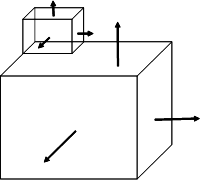
\includegraphics[width=0.9\textwidth, height=0.9\textheight, keepaspectratio=true]{media/image003.png}
\caption{Building heat transfer surfaces cast shadows in the direction of outward facing normal. \protect \label{fig:building-heat-transfer-surfaces-cast-shadows}}
\end{figure}

\begin{figure}[hbtp] % fig 4
\centering
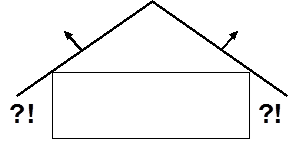
\includegraphics[width=0.9\textwidth, height=0.9\textheight, keepaspectratio=true]{media/image004.png}
\caption{Extended roof surface will not shade the walls below. \protect \label{fig:extended-roof-surface-will-not-shade}}
\end{figure}

Figure~\ref{fig:proper-surface-configurations-for-roof} shows the proper surface configurations for two types of attic construction. In all cases, the roof surface should only include the area of the roof which contacts the zone below it. In these drawings, this is an unconditioned attic space, but it could also be a conditioned zone. Any extensions of the roof which are exposed to the outdoors on both sides should be described as a shading surface.

For the configuration on the left, the overhang should be a shading surface which will cast shadows in both directions (if the default mirroring is disabled the shading surface must face downward). This ensures that the correct shading will be modeled, and it also avoids overstating the heat transfer through the roof into the attic.

For the configuration on the right, the attic is fully enclosed with building heat transfer surfaces for the roof and soffits. The soffits would be described as floor surfaces in the attic and would face downward. The central portion of the attic floor would be described as an interzone floor surface where the outside boundary condition is the ceiling surface in the zone below.

\begin{figure}[hbtp] % fig 5
\centering
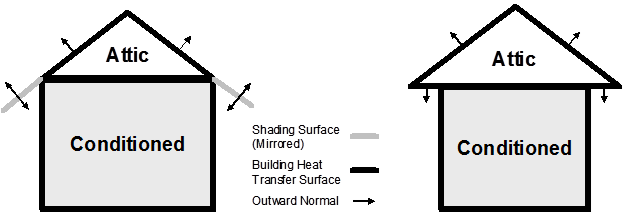
\includegraphics[width=0.9\textwidth, height=0.9\textheight, keepaspectratio=true]{media/image005.png}
\caption{Proper surface configurations for roof overhangs for two types of attic construction. \protect \label{fig:proper-surface-configurations-for-roof}}
\end{figure}


\section{Solar Reflection from Shading Surfaces}\label{solar-reflection-from-shading-surfaces}

Exterior shading surfaces modeled using ``FullInteriorAndExteriorWithReflections'' can show some sky diffuse solar getting through the shades. When ``*WithReflections'' is active a partially sunlit shading surface reflects uniformly from the entire surface. If using WithReflections, shading surfaces should be broken into multiple surfaces at lines of intersection with other shading surfaces. This also includes places where another surface may tee into a shading surface.

For example, a building is shaded by surfaces A, B, and C. Shading Surface A intercepts with Shading Surfaces B and C, and are broken into three areas A1, A2, and A3. Surface A should be entered as the shown three shading areas in order to correctly model sky diffuse solar reflection from Shading Surface A.

\begin{figure}[hbtp] % fig 6
\centering
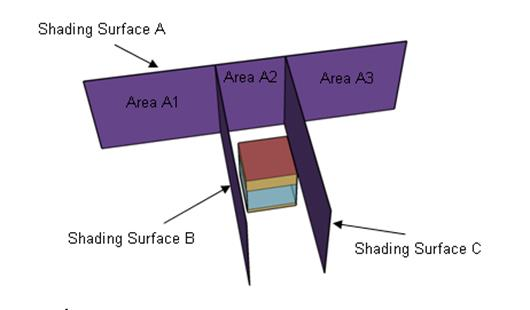
\includegraphics[width=0.9\textwidth, height=0.9\textheight, keepaspectratio=true]{media/image006.jpg}
\caption{Limitations in modeling reflections from surfaces \protect \label{fig:limitations-in-modeling-reflections-from}}
\end{figure}


\section{Air wall, Open air connection between zones}\label{air-wall-open-air-connection-between-zones}

It is extremely difficult to model the interactions between thermal zones which are connected by a large opening. If the zones are controlled to the same conditions, then there is little to be gained by making them interact, so you could neglect any connections between the zones. In fact, if this is the case, you might consider combining the spaces into a single thermal zone. If you expect the zones to have significantly different temperatures and/or humidities, then use one of the following options. If they are modeled as separate zones, EnergyPlus models only what is explicitly described in the input file, so simply leaving a void (no surfaces) between two zones will accomplish nothing - the two zones will not be connected. The main interactions which occur across the dividing line between two zones which are fully open to each other are:

1)~~~Convection or airflow, which will transfer both sensible heat and moisture. Some modelers use MIXING (one-way flow) or CROSS MIXING (two-way flow) to move air between the zones, but the user must specify airflow rates and schedules for this flow, and it cannot be automatically linked to HVAC system operation. Other modelers use AirFlowNetwork with large vertical openings between the zones as well as other openings and cracks in the exterior envelope to provide the driving forces. It can also be connected with the HVAC system (for limited system types). This requires a much higher level of detailed input and should be used only if the detailed specification data is available. If the two zones are controlled to similar conditions, this effect could be safely neglected.

2)~~~Solar gains and daylighting. The only way to pass solar and daylight from one zone to the next is through a window or glass door described as a subsurface on an interzone wall surface. Note that all solar is diffuse after passing through an interior window.

3)~~~Radiant (long-wave thermal) transfer. There is currently no direct radiant exchange between surfaces in different thermal zones. Windows in EnergyPlus are opaque to direct radiant exchange, so an interzone window will not behave any differently than an opaque interzone surface for this aspect. However, a large interzone surface (opaque or window) would result in some indirect radiant exchange since the interzone surface will exchange directly with surfaces in zone A and in zone B. The surface thermal resistance should be low in order to most closely approximate this effect.

4)~~~Conduction. If an interzone surface is placed between the two zones, it will conduct sensible heat between the two zones. Using a low thermal resistance helps to move radiant exchange between the zones.

5)~~~~Visible and thermal radiant output from internal gains. These gains will not cross zone boundaries. But again, they will impact any interzone surfaces, so some of the energy may move across to the next zone."


\section{Daylight Modeling}\label{daylight-modeling}

\emph{Why isn't my lighting energy being reduced with a daylighting system?}

In order to see changes in the lighting electric power consumption due to daylighting, the Fraction Replaceable in the \textbf{Lights} input object must be set to 1.0. This is documented in the I/O reference, and also a warning is generated in the ERR file.


\section{Rain Flag}\label{rain-flag}

\emph{Why is my exterior convection coefficient value 1000?}

When the outside environment indicates that it is raining, the exterior surfaces (exposed to wind) are assumed to be wet. The convection coefficient is set to a very high number (1000) and the outside temperature used for the surface will be the wet-bulb temperature. (If you choose to report this variable, you will see 1000 as its value.)


\section{Interzone Exterior Convection}\label{interzone-exterior-convection}

\emph{Why is my exterior convection coefficient value 0?}

When two surfaces are linked as interzone surfaces, the ``exterior'' side of these surfaces does not really exist. EnergyPlus links the two surfaces by using the inside temperature of surface A as the outside temperature of surface B, and the reverse. For example:

Zone1WestWall has an outside boundary of Surface = Zone2EastWall

Zone2EastWall has an outside boundary of Surface = Zone1WestWall

Let's say that at hour 2, the inside surface temperature of Zone1WestWall is 19C, and the inside temperature of Zone2EastWall is 22C. When the heat balance is calculated for Zone1WestWall, its outside surface temperature will be set to 22C. Likewise, when the heat balance is calculated for Zone2EastWall, its outside surface temperature will be set to 19C. So, for interzone surfaces, h ext does not apply. That is why it is reported as zero.


\section{Modeling Reflective Radiant Barriers}\label{modeling-reflective-radiant-barriers}

\emph{Can EnergyPlus model reflective radiant barriers?}

\begin{enumerate}
\def\labelenumi{\arabic{enumi}.}
\tightlist
\item
  For radiant barriers which are exposed to a thermal zone, such as an attic space, specify a reduced thermal absorptance for the innermost material layer.
\end{enumerate}

For example, an attic roof construction might be (outer to inner)

\begin{lstlisting}

Asphalt shingles,
  R-30 insulation,
  Radiant barrier;
\end{lstlisting}

The radiant barrier material would be a thin layer with some small resistance with a low thermal absorptance value. This will reduce the radiant heat transfer from the roof surface to other surfaces in the attic zone.

\begin{enumerate}
\def\labelenumi{\arabic{enumi}.}
\setcounter{enumi}{1}
\tightlist
\item
  If the radiant barrier is within a cavity which is not modeled as a separate thermal zone, then there is not an easy way to model its impact. For example, a wall construction:
\end{enumerate}

\begin{lstlisting}

Brick,
  R-12 insulation,
  Radiant barrier,
  Air gap,
  Gypsum board;
\end{lstlisting}

Here, the radiant barrier would reduce the radiant transfer across the air gap. But EnergyPlus air gaps are a fixed thermal resistance, specified in the Material:Airgap object. The user would need to compute an average effective resistance which represents the reduced radiant heat transfer across the air gap due to the radiant barrier. This resistance could then be assigned to the radiant barrier material layer.


\section{Cavity Algorithm Model}\label{cavity-algorithm-model}

\emph{Reading the documentation, I'm wondering if the Cavity algorithm is usable for other double facade types or only Trombe wall?~ In other words, does Cavity implicitly presume that the inner wall is highly solar absorbent and so generate specific convection?}

The Trombe wall convection algorithm is applicable to just about any vertical cavity with a high aspect ratio and relatively narrow width. I'm not sure if a double facade cavity would meet the aspect ratio requirement. But I do know the Trombe wall algorithm is not picky about whether the inner wall is highly absorbant, or about any particular properties of the walls. Actually the same basic algorithm is used by the window model to calculate the convection between the two panes of a window. The full reference is ISO 15099.


\section{Using Multipliers (Zone and/or Window)}\label{using-multipliers-zone-andor-window}

\subsection{Background and Study using Multipliers}\label{background-and-study-using-multipliers}

Multipliers are used in EnergyPlus for convenience in modeling. Though window multipliers are useful for any size building when you have multiple windows on a façade, zone multipliers are more useful in large buildings with several to many stories.

Zone multipliers are designed as a ``multiplier'' for floor area, zone loads, and energy consumed by internal gains. It takes the calculated load for the zone and multiplies it, sending the multiplied load to the attached HVAC system. The HVAC system size is specified to meet the entire multiplied zone load and will report the amount of the load met in the Zone/Sys Sensible Heating or Cooling Energy/Rate report variable. Autosizing automatically accounts for multipliers. Metered energy consumption by internal gains objects such as Lights or Electric Equipment will be multiplied.

To illustrate the benefits (and comparison of results), the MultiStory.idf example file was used. The MultiStory file is a 9 zone, 10 story/floored building with heating (ZoneHVAC:Baseboard:Convective:Electric object) and cooling (ZoneHVAC:WindowAirConditioner object). The middle zone of each floor in the original represents 4 zones (multiplier = 4) and the middle floor (ZoneGroup) represents 8 floors (ZoneGroup multiplier = 8). Clone representations were made for comparisons:

\begin{figure}[hbtp] % fig 7
\centering
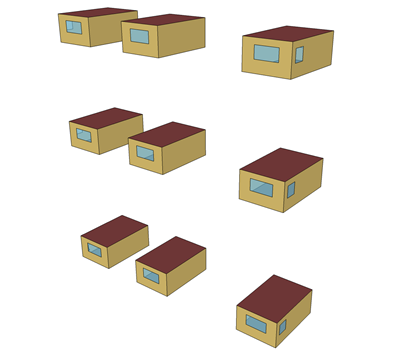
\includegraphics[width=0.9\textwidth, height=0.9\textheight, keepaspectratio=true]{media/image007.png}
\caption{Original Multistory IDF \protect \label{fig:original-multistory-idf}}
\end{figure}

In the figure above, each ``middle'' zone represents 4 zones.~ The middle ``floor'' represents 8 floors. Additionally, each of the windows has a multiplier of 4 -- so each window represents 4 windows of the same size. For the Multistory file, the Zone object for the center zones has the multiplier of 4. And for the center floors, the ZoneList and ZoneGroup objects to collect the zones and apply multipliers. The top floor then uses the Zone object multiplier for the center zones. Specifically:

\begin{lstlisting}

<snip>
    Zone,
      Gnd Center Zone,         !- Name
      0.0,                     !- Direction of Relative North {deg}
      8.0, 0.0, 0.0,           !- Origin [X,Y,Z] {m}
      1,                       !- Type
      4,                       !- Multiplier
      autocalculate,           !- Ceiling Height {m}
      autocalculate;           !- Volume {m3}
  <snip>

    ZoneGroup,
      Mid Floor,               !- Zone Group Name
      Mid Floor List,          !- Zone List Name
      8;                       !- Zone List Multiplier


    ZoneList,
      Mid Floor List,          !- Zone List Name
      Mid West Zone,           !- Zone 1 Name
      Mid Center Zone,         !- Zone 2 Name
      Mid East Zone;           !- Zone 3 Name
  <snip>

    Zone,
      Top Center Zone,         !- Name
      0.0,                     !- Direction of Relative North {deg}
      8.0,                     !- X Origin {m}
      0.0,                     !- Y Origin {m}
      22.5,                    !- Z Origin {m}
      1,                       !- Type
      4,                       !- Multiplier
      autocalculate,           !- Ceiling Height {m}
      autocalculate;           !- Volume {m3}
\end{lstlisting}

For comparison purposes, clones of the middle zones were done.

\begin{figure}[hbtp] % fig 8
\centering
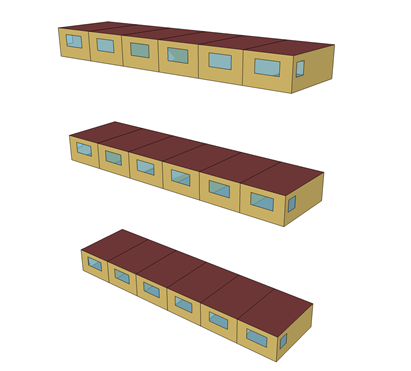
\includegraphics[width=0.9\textwidth, height=0.9\textheight, keepaspectratio=true]{media/image008.png}
\caption{Multistory with cloned middle zones. \protect \label{fig:multistory-with-cloned-middle-zones.}}
\end{figure}

And, finally, the entire building was created:

\begin{figure}[hbtp] % fig 9
\centering
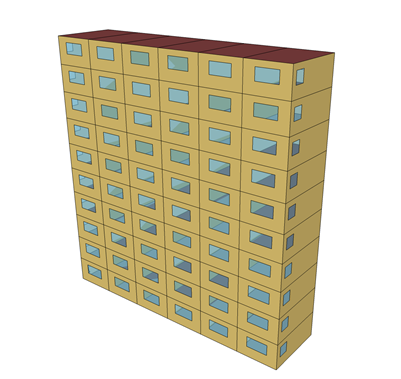
\includegraphics[width=0.9\textwidth, height=0.9\textheight, keepaspectratio=true]{media/image009.png}
\caption{Multistory building -- fully cloned. \protect \label{fig:multistory-building-fully-cloned.}}
\end{figure}

The building is autosized. For convenience in comparison, the extreme summer and winter days were used for autosizing and the simulation was run for the 5 United States weather files that are included in the EnergyPlus release: Chicago IL; San Francisco CA; Golden CO; Tampa FL; and Washington DC.

Comparisons were done with the Zone Group Loads values (Zone Group Sensible Heating Energy and Zone Group Sensible Cooling Energy) as well as meter values for Electricity. Using the regression testing limits that are used during EnergyPlus development testing (i.e.~small differences are within .001 or .5\%; big differences are greater than those limits).

For the purposes of dicussion, the buildings will be called: Multistory 1 -- the original 9 zone building (with multipliers and groups) ref: Figure~\ref{fig:original-multistory-idf}; Multistory 2 -- the building shown in Figure~\ref{fig:multistory-with-cloned-middle-zones.}. Multistory with cloned middle zones.; Multistory 3 -- the fully configured building -- ref Figure~\ref{fig:multistory-building-fully-cloned.}.

The following table illustrates the regression testing for Multistory 2 and Multistory 3, group loads and meters versus Multistory 1 results.

% table 1
\begin{longtable}[c]{p{1.2in}p{1.2in}p{1.2in}p{1.2in}p{1.2in}}
\caption{Multistory vs Multistory 2 and Multistory 3 \label{table:multistory-vs-multistory-2-and-multistory-3}} \tabularnewline
\toprule 
LOCATION & MULTI-STORY 2 LOADS & MULTI-STORY 2 METER & MULTI-STORY 3 LOADS & MULTI-STORY 3 METER \tabularnewline
\midrule
\endfirsthead

\caption[]{Multistory vs Multistory 2 and Multistory 3} \tabularnewline
\toprule 
LOCATION & MULTI-STORY 2 LOADS & MULTI-STORY 2 METER & MULTI-STORY 3 LOADS & MULTI-STORY 3 METER \tabularnewline
\midrule
\endhead

USA\_IL\_Chicago-OHare.Intl.AP.725300\_TMY3 & Small Diffs & Equal & Big Diffs* (76\%) & Big Diffs* (62\%) \tabularnewline
USA\_CA\_San.Francisco.Intl.AP.724940\_TMY3 & Big Diffs* (2.43\%) & Big Diffs* (0.6\%) & Big Diffs* (49\%) & Big Diffs* (41\%) \tabularnewline
USA\_CO\_GOLDEN-NREL.724666\_TMY3 & Small Diffs & Small Diffs & Big Diffs* (26\%) & Big Diffs* (24\%) \tabularnewline
USA\_FL\_Tampa.Intl.AP.722110\_TMY3 & Small Diffs & Small Diffs & Big Diffs* (6\%) & Big Diffs* (2\%) \tabularnewline
USA\_VA\_Sterling-Washington.Dulles.Intl.AP.724030\_TMY3 & Equal & Equal & Big Diffs* (91\%) & Big Diffs* (72\%) \tabularnewline
\bottomrule
\end{longtable}

* Big Diffs maximum occur in monthly values whereas the runperiod values are much smaller.

To try to pare down the discrepancies shown here, the effects of height that are used in the calculations were removed (i.e., the Site:WeatherStation and Site:HeightVariation objects were entered as below to negate the effects of height on the environmental variables such as wind and temperature).~ In addition the height effect was removed from the OutdoorAir:Node object.

\begin{lstlisting}

  Site:WeatherStation,
      ,          !- Wind Sensor Height Above Ground {m}
      ,          !- Wind Speed Profile Exponent
      ,          !- Wind Speed Profile Boundary Layer Thickness {m}
      0;         !- Air Temperature Sensor Height Above Ground {m}


    Site:HeightVariation,
      0,         !- Wind Speed Profile Exponent
      ,          !- Wind Speed Profile Boundary Layer Thickness {m}
      0;         !- Air Temperature Gradient Coefficient {K/m}
\end{lstlisting}

Figure 10. Objects removing height from building impacts.

With these included, the files were rerun with the following results:

% table 2
\begin{longtable}[c]{p{1.2in}p{1.2in}p{1.2in}p{1.2in}p{1.2in}}
\caption{Multiplier Results with negated height variation. \label{table:multiplier-results-with-negated-height}} \tabularnewline
\toprule 
Location & Multi-story 2 Loahs & Multi-story 2 Meter & Multi-story 3 Loahs & Multi-story 3 Meter \tabularnewline
\midrule
\endfirsthead

\caption[]{Multiplier Results with negated height variation.} \tabularnewline
\toprule 
Location & Multi-story 2 Loahs & Multi-story 2 Meter & Multi-story 3 Loahs & Multi-story 3 Meter \tabularnewline
\midrule
\endhead

USA\_IL\_Chicago-OHare.Intl.AP.725300\_TMY3 & Small diffs & Small diffs & Small diffs & Small diffs \tabularnewline
USA\_CA\_San.Francisco.Intl.AP.724940\_TMY3 & Small diffs & Small diffs & Small diffs & Small diffs \tabularnewline
USA\_CO\_GOLDEN-NREL.724666\_TMY3 & Small diffs & Small diffs & Small diffs & Small diffs \tabularnewline
USA\_FL\_Tampa.Intl.AP.722110\_TMY3 & Small diffs & Small diffs & Small diffs & Small diffs \tabularnewline
USA\_VA\_Sterling-Washington.Dulles.Intl.AP.724030\_TMY3 & Small diffs & Small diffs & Small diffs & Small diffs \tabularnewline
\bottomrule
\end{longtable}

To investigate if other systems might have different results, the Ideal Loads System was used as the system.~ Similar results were found for the multipliers vs cloned results. However, it may also be noted that the results between the original systems (baseboard and window ac) vs the ideal loads were very similar.

The biggest difference really comes in calculation time. As shown in the following table,

% table 3
\begin{longtable}[c]{p{1.5in}p{1.5in}p{1.5in}p{1.5in}}
\caption{Runtimes for Multistory files (baseboard/window ac) \label{table:runtimes-for-multistory-files-baseboardwindow}} \tabularnewline
\toprule 
Location & Multi-story 1 (9 zones) (mm:ss) & Multi-story 2~ (18 zones) (MM:SS) & Multi-story 3 (60 zones) (MM:SS) \tabularnewline
\midrule
\endfirsthead

\caption[]{Runtimes for Multistory files (baseboard/window ac)} \tabularnewline
\toprule 
Location & Multi-story 1 (9 zones) (mm:ss) & Multi-story 2~ (18 zones) (MM:SS) & Multi-story 3 (60 zones) (MM:SS) \tabularnewline
\midrule
\endhead

USA\_IL\_Chicago-OHare.Intl.AP.725300\_TMY3 & 1:05 & 2:14 & 13:15 \tabularnewline
USA\_CA\_San.Francisco.Intl.AP.724940\_TMY3 & 1:04 & 2:05 & 13:20 \tabularnewline
USA\_CO\_GOLDEN-NREL.724666\_TMY3 & 1:17 & 2:28 & 14:43 \tabularnewline
USA\_FL\_Tampa.Intl.AP.722110\_TMY3 & 1:11 & 2:21 & 13:43 \tabularnewline
USA\_VA\_Sterling-Washington.Dulles.Intl.AP.724030\_TMY3 & 1:05 & 2:15 & 13:18 \tabularnewline
\bottomrule
\end{longtable}

Because the overall results were so similar, the run times for the Ideal Loads runs are included:

% table 4
\begin{longtable}[c]{p{1.5in}p{1.5in}p{1.5in}p{1.5in}}
\caption{Runtime for Multistory files (ideal loads) \label{table:runtime-for-multistory-files-ideal-loads}} \tabularnewline
\toprule 
Location & Multi-story 1 (9 zones) (mm:ss) & Multi-story 2 (18 zones) (MM:SS) & Multi-story 3 (60 zones) (MM:SS) \tabularnewline
\midrule
\endfirsthead

\caption[]{Runtime for Multistory files (ideal loads)} \tabularnewline
\toprule 
Location & Multi-story 1 (9 zones) (mm:ss) & Multi-story 2 (18 zones) (MM:SS) & Multi-story 3 (60 zones) (MM:SS) \tabularnewline
\midrule
\endhead

USA\_IL\_Chicago-OHare.Intl.AP.725300\_TMY3 & 0:51 & 1:34 & 9:37 \tabularnewline
USA\_CA\_San.Francisco.Intl.AP.724940\_TMY3 & 0:50 & 1:34 & 9:59 \tabularnewline
USA\_CO\_GOLDEN-NREL.724666\_TMY3 & 0:51 & 1:40 & 10:31 \tabularnewline
USA\_FL\_Tampa.Intl.AP.722110\_TMY3 & 0:51 & 1:36 & 10:05 \tabularnewline
USA\_VA\_Sterling-Washington.Dulles.Intl.AP.724030\_TMY3 & 0:51 & 1:36 & 9:48 \tabularnewline
\bottomrule
\end{longtable}

More zones (and, particularly more surfaces) make for longer run times.

\subsection{Guidelines for Using Multipliers and Groups}\label{guidelines-for-using-multipliers-and-groups}

\begin{itemize}
\item
  If the basic zone geometry is identical, make one zone, copy \& paste it as necessary, then change the Zone Origin field to locate each zone correctly.
\item
  Do not use interzone surfaces between zones that are multiplied. Set the adjoining surfaces to be adiabatic, i.e.~use the OtherZoneSurface exterior boundary condition with the other surface pointing back to itself.
\item
  Locate the middle floor zones roughly halfway between top and ground because exterior convection coefficients change with height. Halfway should cause the differences to average out. If you have many stories (the example only has 10 stories), consider using more middle floor zones.
\item
  Consider removing the effects of height variation for the simulation.
\item
  Follow guidelines in HVACTemplate and other objects about sizing if you are mixing autosize fields with hard sized fields (recommended to ``autosize'' all fields rather than mix).
\item
  All HVAC system sizes must be specified to meet the entire multiplied zone load.
\item
  Autosizing automatically accounts for multipliers.
\end{itemize}


\section{Using OSC (Other Side Coefficients) to create controlled panels}\label{using-osc-other-side-coefficients-to-create-controlled-panels}

The Other Side Coefficient (OSC) equation permits setting either the outside surface temperature or the outside air temperature to a constant value or a scheduled value based on the size of the first input parameter, N1. The original temperature equation was:

\begin{equation}
T = N_2 T_{zone} + N_3 T_{oadb} + N_4 N_5 + N_6 T_{grnd} + N_7 W_{spd} T_{oadb}
\end{equation}

where:

\begin{itemize}
\item
  \(T\) = Outside Air Temperature when N1 (Combined convective/radiative film Coeff) \textgreater{} 0
\item
  \(T\) = Exterior Surface Temperature when N1 (Combined convective/radiative film Coeff) \textless{} = 0
\item
  \(T_{zone}\) = MAT = Temperature of the zone being simulated (°C)
\item
  \(T_{oadb}\) = Dry-bulb temperature of the outdoor air (°C)
\item
  \(T_{grnd}\) = Temperature of the ground (°C) Wspd = Outdoor wind speed (m/sec)
\end{itemize}

The coefficients N\(_{2}\), N\(_{3}\), N\(_{4}\), N\(_{6}\), and N\(_{7}\) scale the contribution of the various terms that follow them.~ In the case of N\(_{4}\), it is followed by another term N\(_{5}\).~ This is a constant temperature that can also be overridden by a scheduled value. Note that in some EnergyPlus documentation, the N's are given as C's.

This object has been changed to permit the outside temperature, T, to be controlled to a set point temperature that is specified as N\(_{5}\) or comes from the schedule A2.

Note that since the surface that contains the panel subsurfaces (that must be called doors in EnergyPlus) receives that same outside temperature as the panels, it should have a construction with a very high thermal resistance to essentially take it out of the room heat balance calculation.

An Example input file object is shown below.

\begin{lstlisting}

SurfaceProperty:OtherSideCoefficients,
     Zn001:Roof001:OSC, !- Name
     0,   ! (N1) Combined Convective/Radiative Film Coefficient {W/m2-K}
     0,   ! (N5) Constant Temperature {C}
     0.95,!(N4) Constant Temperature Coefficient
     ,    ! (N3)External Dry-Bulb Temperature Coefficient
     ,    ! (N6)Ground Temperature Coefficient
     ,    ! (N7)Wind Speed Coefficient
     -.95,! (N2) Zone Air Temperature Coefficient
     ConstantCooling,     ! (A2) Constant Temperature Schedule Name
     No,  ! (A3)Sinusoidal Variation of Constant Temperature Coefficient
     24,  ! (N8)Period of Sinusoidal Variation {hr}
     1.,  ! (N9)Previous Other Side Temperature Coefficient
     5.,  !(N10) Minimum Other Side Temperature Limit
     25.; ! (N11) Maximum Other Side Temperature Limit
\end{lstlisting}

This object results in the following equation for T:

T = 1.0*Tlast +0.95*(Tsetpoint -- TzoneAir)~~ (with limits)

The result of this is that the surface temperature, T, will be changed to the temperature that will force the zone air temperature to the setpoint providing the temperature limits are not reached. When the zone air temperature is at the setpoint, T remains at the value it had in the prior time step.

A complete example with all pertinent objects:

\begin{lstlisting}

  Construction,
      PanelConst,              !- Name
      Std Steel_Brown_Regular; !- Outside Layer


    Material,
      Std Steel_Brown_Regular, !- Name
      Smooth,                  !- Roughness
      1.5000000E-03,           !- Thickness {m}
      44.96960,                !- Conductivity {W/m-K}
      7689.000,                !- Density {kg/m3}
      418.0000,                !- Specific Heat {J/kg-K}
      0.9000000,               !- Thermal Absorptance
      0.9200000,               !- Solar Absorptance
      0.92000000;              !- Visible Absorptance


    BuildingSurface:Detailed,
      Zn001:Roof001,           !- Name
      Roof,                    !- Surface Type
      ROOF31,                  !- Construction Name
      ZONE ONE,                !- Zone Name
      OtherSideCoefficients,   !- Outside Boundary Condition
      Zn001:Roof001:OSC,       !- Outside Boundary Condition Object
      NoSun,                   !- Sun Exposure
      NoWind,                  !- Wind Exposure
      0,                       !- View Factor to Ground
      4,                       !- Number of Vertices
      0.000000,15.24000,4.572,  !- X,Y,Z = = > Vertex 1 {m}
      0.000000,0.000000,4.572,  !- X,Y,Z = = > Vertex 2 {m}
      15.24000,0.000000,4.572,  !- X,Y,Z = = > Vertex 3 {m}
      15.24000,15.24000,4.572;  !- X,Y,Z = = > Vertex 4 {m}


    FenestrationSurface:Detailed,
      panel002,                !- Name
      Door,                    !- Surface Type
      PanelConst,              !- Construction Name
      Zn001:Roof001,           !- Building Surface Name
      ,                        !- Outside Boundary Condition Object
      autocalculate,           !- View Factor to Ground
      ,                        !- Shading Control Name
      ,                        !- Frame and Divider Name
      1,                       !- Multiplier
      4,                       !- Number of Vertices
      3,2,4.572,  !- X,Y,Z = = > Vertex 1 {m}
      3,3,4.572,  !- X,Y,Z = = > Vertex 2 {m}
      4,3,4.572,  !- X,Y,Z = = > Vertex 3 {m}
      4,2,4.572;  !- X,Y,Z = = > Vertex 4 {m}


    SurfaceProperty:OtherSideCoefficients,
      Zn001:Roof001:OSC,       !- Name
      0,            !- Combined Convective/Radiative Film Coefficient {W/m2-K}
      0,                       !- Constant Temperature {C}
      0.95,                    !- Constant Temperature Coefficient
      ,                        !- External Dry-Bulb Temperature Coefficient
      ,                        !- Ground Temperature Coefficient
      ,                        !- Wind Speed Coefficient
      -.95,                    !- Zone Air Temperature Coefficient
      ConstantTwentyTwo,       !- Constant Temperature Schedule Name
      No,           !- Sinusoidal Variation of Constant Temperature Coefficient
      24,                      !- Period of Sinusoidal Variation {hr}
      1.,                      !- Previous Other Side Temperature Coefficient
      5.,                      !- Minimum Other Side Temperature Limit {C}
      25.;                     !- Maximum Other Side Temperature Limit {C}


  Schedule:Constant,ConstantTwentyTwo,PanelControl,22;
\end{lstlisting}


\chapter{Natural and Mechanical Ventilation}\label{natural-and-mechanical-ventilation}


\section{AirflowNetwork and EarthTube}\label{airflownetwork-and-earthtube}

\emph{When I use an Earthtube with an AirFlowNetwork, I get a ``Orphan Object'' warning.}

Currently, Earthtube and AirFlowNetworks do not work together.~ If both objects co-exist, the AirflowNetwork mode supersedes the Earthtube mode at two control choices. Since this causes the Earthtube objects to not be used, the ``orphan'' warning appears.

There are four control choices in the second field of the AirflowNetwork Simulation object (spaces included for readability)

\begin{itemize}
\item
  MULTIZONE WITH DISTRIBUTION
\item
  MULTIZONE WITHOUT DISTRIBUTION
\item
  MULTIZONE WITH DISTRIBUTION ONLY DURING FAN OPERATION
\item
  NO MULTIZONE OR DISTRIBUTION
\end{itemize}

When the first two choices are selected, the AirflowNetwork model takes over airflow calculation. The earthtube objects are not used in the airflow calculation, causing the ``orphan'' warning. The example file, AirflowNetwork\_Multizone\_SmallOffice.idf, uses the first choice.~ When the second choice is used, the AirflowNetwork model is only used during HVAC operation time. During system off time, the earthtube model is used to calculate airflows.~ Thus, no ``orphan'' warning will be given, but the earthtube may be being used less than expected.~ The example file, AirflowNetwork\_Simple\_House.idf, uses the third choice.


\chapter{HVAC, Sizing, Equipment Simulation and Controls}\label{hvac-sizing-equipment-simulation-and-controls}


\section{HVAC Sizing Tips}\label{hvac-sizing-tips}

To help achieve successful autosizing of HVAC equipment, note the following general guidelines.

\begin{itemize}
\item
  Begin with everything fully autosized (no user-specified values) and get a working system before trying to control any specific sized.
\item
  The user must coordinate system controls with sizing inputs. For example, if the Sizing:System ``Central Cooling Design Supply Air Temperature'' is set to 13C, the user must make sure that the setpoint manager for the central cooling coil controls to 13C as design conditions. EnergyPlus does not cross-check these inputs. The sizing calculations use the information in the Sizing:* objects. The simulation uses the information in controllers and setpoint managers.
\item
  User-specified flow rates will only impact the sizing calculations if entered in the Sizing:Zone or Sizing:System objects. Sizing information flows only from the sizing objects to the components. The sizing calculations have no knowledge of user-specified values in a component. The only exception to this rule is that plant loop sizing will collect all component design water flow rates whether autosized or user-specified.
\item
  The zone thermostat schedules determine the times at which design loads will be calculated. All zone-level schedules (such as lights, electric equipment, infiltration) are active during the sizing calculations (using the day type specified for the sizing period). System and plant schedules (such as availability managers and component schedules) are unknown to the sizing calculations. To exclude certain times of day from the sizing load calculations, use the thermostat setpoint schedules for SummerDesignDay and/or WinterDesignDay. For example, setting the cooling setpoint schedule to 99C during nighttime hours for the SummerDesignDay day type will turn off cooling during those hours.
\end{itemize}

For more information, read the Input Output Reference section on ``Input for Design Calculations and Component Autosizing.''


\section{Variable Refrigerant Flow Air Conditioner}\label{variable-refrigerant-flow-air-conditioner}

\textbf{\emph{The EnergyPlus v7.0 release (October 2011) includes an initial model for VRF systems.~ See AirConditioner:VariableRefrigerantFlow and related objects.}}

\emph{Can I model a VRV or VRF system in EnergyPlus?}

Variable Refrigerant Flow (VRF, or Variable Refrigerant Volume - VRV) air conditioners are available in EnergyPlus V7 and later.

Otherwise, the closest model available would be the multi-speed cooling and heating AC (AirLoopHVAC:UnitaryHeatPump:AirToAir:MultiSpeed used with Coil:Cooling:DX:Multispeed and Coil:Heating:DX:Multispeed coils). This model will provide information for cooling-only or heating-only operation (VRF heat pump mode).

Others have attempted to simulate a VRF system with the existing VAV model. This model will only provide valid information when cooling is required. The results will only be as good as the DX cooling coil performance curves allow. The heating side of a VAV system does not use a DX compression system (i.e., uses gas or electric heat) so this part of the VRV system cannot be modeled with a VAV system.

Note that using either of these models will not provide accurate results since each of these system types provides conditioned air to all zones served by the HVAC system. The VAV system terminal unit may be set to use a minimum flow of 0 where the resulting air flow to that zone is 0 when cooling is not required. Energy use in this case may be slightly more accurate.


\section{Modeling Desiccant DeHumidifiers}\label{modeling-desiccant-dehumidifiers}

\emph{How do I enter performance data for a desiccant dehumidifier?}

It depends on which specific EnergyPlus object you are trying to use.

The Dehumidifier:Desiccant:NoFans object has default performance curves within the model itself that you can use.~ Set field A12, ``Performance Model,'' to DEFAULT.~ Alternatively, you could also obtain manufacturer's data and develop your own curve fits, then set ``Performance Model'' to User Curves.~~ See the Input Output Reference for more details.

If you want to use the Dehumidifier:Desiccant:System object, then some data set inputs for the required HeatExchanger:Desiccant:BalancedFlow:PerformanceDataType1 object are contained in the file ``PerfCurves.idf'' in the DataSets folder.~ You could also obtain manufacturer's data and develop your own inputs for the HeatExchanger:Desiccant:BalancedFlow:PerformanceDataType1 object.


\section{Boiler Control Schedule}\label{boiler-control-schedule}

\emph{How can I get my boiler to only work when the outdoor temperature is less than 5°C?}

To schedule the boiler to work only when the outdoor dry bulb temperature is below 5°C, create two schedules based on the temperatures in the weather file. You can do this by reporting Outdoor Dry Bulb hourly, then make a spreadsheet with two columns, one which = 1 whenever ODB≥5, and the other which = 1 whenever ODB \textless{} 5. Save this spreadsheet as a csv format file, and then you can use Schedule:File to read these as EnergyPlus schedules. Use these schedules in the PlantEquipmentOperationSchemes object to make ``boiler heating'' active in cold weather and ``heatpump Heating'' active in warmer weather.

Note that you will need to have two PlantEquipmentList objects, one which lists only the boiler, and the other which lists only the heat pump. And the two different PlantEquipmentOperation:HeatingLoad objects should reference different PlantEquipmentList objects.

Report temperatures and flow rates at selected points on the hot water loop to see if things are working properly.


\section{Difference between EIR and Reformulated EIR Chillers}\label{difference-between-eir-and-reformulated-eir-chillers}

\emph{What is the difference between the EIR and ReformulatedEIR models of Electric Chillers?~ I am getting strange results.}

The COP of a chiller is a function of part load ratio. It is mainly determined by the Energy Input to Cooling Output Ratio Function of Part Load Ratio Curve.~ When the EIR model is used for an electric chiller, the curve has an independent variable: part load ratio.~ For the ReformulatedEIR model, the curve requires two independent variables: leaving condenser water temperature and part load ratio.~ Each independent variable has its min and max values. If a variable is outside the allowed range, the nearest allowed value is used, possibly resulting in an unexpected result.

If you would like to compare COP values for two types of chillers, you may need to ensure that the same conditions are applied. For simplicity, you may want to use a spreadsheet to calculate the curve values.


\section{Using Well Water}\label{using-well-water}

The water-to-water heat pumps have not been programmed to allow well water. However, cooling towers have (see 5ZoneWaterSystems.idf) and you should be able to connect the WSHP to a condenser loop with a cooling tower.

Currently, there is no method to directly simulate well water as the condensing fluid for water source heat pumps. So to get as close as possible, program the cooling towers to allow well water via the water use object. If the cooling tower inlet node water temperature represents the well water temperature, and if you can set up the cooling tower to provide an outlet water temperature very close to the inlet water temperature, then this would be the same as connecting the well water directly to the WSHP. Minimize the cooling tower fan energy or disregard it completely when performing your simulation. Use report variables at the inlet/outlet node of the cooling tower to investigate how close you can get to your equipment configuration.


\section{Plant Load Profile}\label{plant-load-profile}

The Plant Load Profile object is used to ``pass'' a load to the plant where the plant meets this load. The load profile places an inlet and outlet water temperature and a mass flow rate at the inlet to the plant loop. This is where you will need to focus when you try to alter the boiler performance.


\section{HVAC System Turn Off}\label{hvac-system-turn-off}

\emph{My HVAC system won't turn off even when my availability schedule is 0 (off).}

The night cycle option is set to Cycle On Any in the HVACTemplate:System:Unitary object. This will turn on the AC system. Change the night cycle option to Stay Off and the system shuts down correctly. For future reference, an indicator of night cycle operation is the on one time step, off the next type of operation.


\section{Fan Types}\label{fan-types}

\emph{I am confused about the differences between the different fan types.~ Can you explain?}

In short:

Fan:ConstantVolume is a constant volume, continuous operation fan which can be turned on and off via a schedule.

Fan:OnOff is similar to the one above, but it cycles itself on and off as required by its thermostat \ldots{} all during the scheduled operation period. This is a typical mode of operation for a home furnace.

Fan:VariableVolume runs continuously during the Schedule period, but varies its volume to meet the heating or cooling demand.

Consult the \href{file:///E:/Docs4PDFs/InputOutputReference.pdf}{Input Output Reference document} (group Fans) for additional information.


\section{Use of Set Point Managers}\label{use-of-set-point-managers}

A coil will check its inlet air temperature compared to the set point temperature. For cooling, if the inlet air temperature is above the set point temp, the coil turns on. It's opposite that for heating. In the 5ZoneAutoDXVAV example file, a schedule temperature set point is placed at the system outlet node. This is the temperture the designer wants at the outlet. The mixed air SP manager is used to account for fan heat and places the required SP at the outlet of the cooling coil so the coil slightly overcools the air to overcome fan heat and meet the system outlet node set point.

You don't blindly place the SP's at the coil outlet node, but this is a likely starting point in most cases. If there is a fan after the coil's, the ``actual'' SP will need to be placed on a different node (other than the coils). Then a mixed air manager will be used to reference that SP and the fan's inlet/outlet node to calculate the correct SP to place wherever you want (at the coil outlet, the mixed air node, etc.). Place it at the mixed air node if you want the outside air system to try and meet that setpoint through mixing. Place it at the cooling coil outlet if you want the coil control to account for fan heat. Place it at both locations if you want the outside air system to try and meet the load with the coil picking up the remainder of the load.

See if the coils are fully on when the SP is not met. If they are the coils are too small. If they are at part-load, the control SP is calculated incorrectly.

\subsection{Relationship of Set Point Managers and Controllers}\label{relationship-of-set-point-managers-and-controllers}

\emph{Could you elaborate further on the relation between SetPoint managers and Controllers?}

SetpointManager objects place a setpoint on a node, for example, one might place a setpoint of 12C on the node named ``Main Cooling Coil Air Outlet Node''.

In the case of Controler:WaterCoil which controls a hot water or chilled water coil, the controller reads the setpoint and tries to adjust the water flow so that the air temperature at the controlled node matches the current setpoint.~ Continuing the example above:

\begin{lstlisting}

  Controller:WaterCoil,
      Main Cooling Coil Controller,  !- Name
      Temperature,                   !- Control variable
      Reverse,                       !- Action
      Flow,                          !- Actuator variable
      Main Cooling Coil Air Outlet Node,   !- Control_Node
      Main Cooling Coil Water Inlet Node,  !- Actuator_Node
      0.002,                         !- Controller Convergence Tolerance:
                                     !- delta temp from setpoint temp {deltaC}
      autosize,                      !- Max Actuated Flow {m3/s}
      0.0;                           !- Min Actuated Flow {m3/s}
\end{lstlisting}

It is possible to place the control node downstream of the actual object being controlled, for example after other coils and the supply fan, but I recommend using the coil leaving air node as the control node for tighter control.


\section{HVAC Availability Schedules}\label{hvac-availability-schedules}

\emph{How do availability schedules work?}

Apply the availability schedule to the HVAC System (i.e., Furnace or DXSystem), the coils and the fan objects. If compact HVAC objects are used, apply the availability schedule to the compact HVAC object. You will get different results depending on the selection for the night cycle option.


\section{HVAC System Types}\label{hvac-system-types}

\emph{What kind of systems are available in EnergyPlus?}

EnergyPlus HVAC systems input is flexible, so many different types of systems can be built using the basic available components. There are also compound components which represent common equipment types, and HVACTemplate systems which simplify the input for specific systems. This list gives an overview of HVAC objects in EnergyPlus:

HVAC Templates

\begin{itemize}
\tightlist
\item
  HVACTemplate:Thermostat
\item
  HVACTemplate:Zone:IdealLoadsAirSystem
\item
  HVACTemplate:Zone:FanCoil
\item
  HVACTemplate:Zone:PTAC
\item
  HVACTemplate:Zone:PTHP
\item
  HVACTemplate:Zone:Unitary
\item
  HVACTemplate:Zone:VAV
\item
  HVACTemplate:Zone:VAV:FanPowered
\item
  HVACTemplate:Zone:WaterToAirHeatPump
\item
  HVACTemplate:System:Unitary
\item
  HVACTemplate:System:Unitary:AirToAir
\item
  HVACTemplate:System:VAV
\item
  HVACTemplate:System:PackagedVAV
\item
  HVACTemplate:System:DedicatedOutdoorAir
\item
  HVACTemplate:Plant:ChilledWaterLoop
\item
  HVACTemplate:Plant:Chiller
\item
  HVACTemplate:Plant:Tower
\item
  HVACTemplate:Plant:HotWaterLoop
\item
  HVACTemplate:Plant:Boiler
\item
  HVACTemplate:Plant:MixedWaterLoop
\end{itemize}

Zone HVAC Forced Air Units

\begin{itemize}
\tightlist
\item
  ZoneHVAC:IdealLoadsAirSystem
\item
  ZoneHVAC:FourPipeFanCoil
\item
  ZoneHVAC:WindowAirConditioner
\item
  ZoneHVAC:PackagedTerminalAirConditioner
\item
  ZoneHVAC:PackagedTerminalHeatPump
\item
  ZoneHVAC:WaterToAirHeatPump
\item
  ZoneHVAC:Dehumidified:DX
\item
  ZoneHVAC:EnergyRecoveryVentilator
\item
  ZoneHVAC:EnergyRecoveryVentilator:Controller
\item
  ZoneHVAC:UnitVentilator
\item
  ZoneHVAC:UnitHeater
\item
  ZoneHVAC:OutdoorAirUnit
\item
  ZoneHVAC:TerminalUnit:VariableRefrigerantFlow
\end{itemize}

Zone HVAC Radiative/Convective Units

\begin{itemize}
\tightlist
\item
  ZoneHVAC:Baseboard:RadiantConvective:Water
\item
  ZoneHVAC:Baseboard:RadiantConvective:Steam
\item
  ZoneHVAC:Baseboard:RadiantConvective:Electric
\item
  ZoneHVAC:Baseboard:Convective:Water
\item
  ZoneHVAC:Baseboard:Convective:Electric
\item
  ZoneHVAC:LowTemperatureRadiant:VariableFlow
\item
  ZoneHVAC:LowTemperatureRadiant:ConstantFlow
\item
  ZoneHVAC:LowTemperatureRadiant:Electric
\item
  ZoneHVAC:HighTemperatureRadiant
\item
  ZoneHVAC:VentilatedSlab
\end{itemize}

Zone HVAC Air Loop Terminal Units

\begin{itemize}
\tightlist
\item
  AirTerminal:SingleDuct:Uncontrolled
\item
  AirTerminal:SingleDuct:ConstantVolume:Reheat
\item
  AirTerminal:SingleDuct:VAV:NoReheat
\item
  AirTerminal:SingleDuct:VAV:Reheat
\item
  AirTerminal:SingleDuct:VAV:Reheat:VariableSpeedFan
\item
  AirTerminal:SingleDuct:VAV:HeatAndCool:NoReheat
\item
  AirTerminal:SingleDuct:VAV:HeatAndCool:Reheat
\item
  AirTerminal:SingleDuct:SeriesPIU:Reheat
\item
  AirTerminal:SingleDuct:ParallelPIU:Reheat
\item
  AirTerminal:SingleDuct:ConstantVolume:FourPipeInduction
\item
  AirTerminal:SingleDuct:ConstantVolume:FourPipeBeam
\item
  AirTerminal:SingleDuct:ConstantVolume:CooledBeam
\item
  AirTerminal:DualDuct:ConstantVolume
\item
  AirTerminal:DualDuct:VAV
\item
  AirTerminal:DualDuct:VAV:OutdoorAir
\item
  ZoneHVAC:AirDistributionUnit
\end{itemize}

Fans

\begin{itemize}
\tightlist
\item
  Fan:ConstantVolume
\item
  Fan:VariableVolume
\item
  Fan:OnOff
\item
  Fan:ZoneExhaust
\item
  FanPerformance:NightVentilation
\item
  Fan:ComponentModel
\end{itemize}

Coils

\begin{itemize}
\tightlist
\item
  Coil:Cooling:Water
\item
  Coil:Cooling:Water:DetailedGeometry
\item
  Coil:Cooling:DX:SingleSpeed
\item
  Coil:Cooling:DX:TwoSpeed
\item
  Coil:Cooling:DX:MultiSpeed
\item
  Coil:Cooling:DX:TwoStageWithHumidityControlMode
\item
  CoilPerformance:DX:Cooling
\item
  Coil:Cooling:DX:VariableRefrigerantFlow
\item
  Coil:Heating:DX:VariableRefrigerantFlow
\item
  Coil:Heating:Water
\item
  Coil:Heating:Steam
\item
  Coil:Heating:Electric
\item
  Coil:Heating:Fuel
\item
  Coil:Heating:Desuperheater
\item
  Coil:Heating:DX:SingleSpeed
\item
  Coil:Heating:DX:MultiSpeed
\item
  Coil:Cooling:WaterToAirHeatPump:ParameterEstimation
\item
  Coil:Heating:WaterToAirHeatPump:ParameterEstimation
\item
  Coil:Cooling:WaterToAirHeatPump:EquationFit
\item
  Coil:Cooling:WaterToAirHeatPump:VariableSpeedEquationFit
\item
  Coil:Heating:WaterToAirHeatPump:EquationFit
\item
  Coil:Heating:WaterToAirHeatPump:VariableSpeedEquationFit
\item
  Coil:WaterHeating:AirToWaterHeatPump
\item
  Coil:WaterHeating:Desuperheater
\item
  CoilSystem:Cooling:DX
\item
  CoilSystem:Heating:DX
\item
  CoilSystem:Cooling:Water:HeatExchangerAssisted
\item
  CoilSystem:Cooling:DX:HeatExchangerAssisted
\end{itemize}

Evaporative Coolers

\begin{itemize}
\tightlist
\item
  EvaporativeCooler:Direct:CelDekPad
\item
  EvaporativeCooler:Indirect:CelDekPad
\item
  EvaporativeCooler:Indirect:WetCoil
\item
  EvaporativeCooler:Indirect:ResearchSpecial
\end{itemize}

Humidifiers and Dehumidifiers

\begin{itemize}
\tightlist
\item
  Humidifier:Steam:Electric
\item
  Dehumidifier:Desiccant:NoFans
\item
  Dehumidifier:Desiccant:System
\end{itemize}

Heat Recovery

\begin{itemize}
\tightlist
\item
  HeatExchanger:AirToAir:FlatPlate
\item
  HeatExchanger:AirToAir:SensibleAndLatent
\item
  HeatExchanger:Desiccant:BalancedFlow
\item
  HeatExchanger:Desiccant:BalancedFlow:PerformanceDataType1
\end{itemize}

Unitary Equipment

\begin{itemize}
\tightlist
\item
  AirLoopHVAC:Unitary:Furnace:HeatOnly
\item
  AirLoopHVAC:Unitary:Furnace:HeatCool
\item
  AirLoopHVAC:UnitaryHeatOnly
\item
  AirLoopHVAC:UnitaryHeatCool
\item
  AirLoopHVAC:UnitaryHeatPump:AirToAir
\item
  AirLoopHVAC:UnitaryHeatPump:WaterToAir
\item
  AirLoopHVAC:UnitaryHeatCool:VAVChangeoverBypass
\item
  AirLoopHVAC:UnitaryHeatPump:AirToAir:MultiSpeed
\end{itemize}

Variable Refrigerant Flow Equipment

\begin{itemize}
\tightlist
\item
  AirConditioner:VariableRefrigerantFlow
\end{itemize}

Air Distribution

\begin{itemize}
\tightlist
\item
  AirLoopHVAC
\item
  AirLoopHVAC:OutdoorAirSystem:EquipmentList
\item
  AirLoopHVAC:OutdoorAirSystem
\item
  OutdoorAir:Mixer
\item
  AirLoopHVAC:ZoneSplitter
\item
  AirLoopHVAC:SupplyPlenum
\item
  AirLoopHVAC:SupplyPath
\item
  AirLoopHVAC:ZoneMixer
\item
  AirLoopHVAC:ReturnPlenum
\item
  AirLoopHVAC:ReturnPath
\end{itemize}

Pumps

\begin{itemize}
\tightlist
\item
  Pump:VariableSpeed
\item
  Pump:ConstantSpeed
\item
  Pump:VariableSpeed:Condensate
\item
  HeaderedPumps:VariableSpeed
\item
  HeaderedPumps:ConstantSpeed
\end{itemize}

Solar Collectors

\begin{itemize}
\tightlist
\item
  SolarCollectorPerformance:FlatPlate
\item
  SolarCollector:FlatPlate:Water
\item
  SolarCollector:FlatPlate:PhotovoltaicThermal
\item
  SolarCollectorPerformance:PhotovoltaicThermal:Simple
\item
  SolarCollector:IntegralCollectorStorage
\item
  SolarCollectorPerformance:IntegralCollectorStorage
\item
  SolarCollector:UnglazedTranspired
\item
  SolarCollector:UnglazedTranspired:Multisystem
\end{itemize}

Plant Heating and Cooling Equipment

\begin{itemize}
\tightlist
\item
  Boiler:HotWater
\item
  Boiler:Steam
\item
  Chiller:Electric:EIR
\item
  Chiller:Electric:ReformulatedEIR
\item
  Chiller:Electric
\item
  Chiller:Absorption:Indirect
\item
  Chiller:Absorption
\item
  Chiller:ConstantCOP
\item
  Chiller:EngineDriven
\item
  Chiller:CombustionTurbine
\item
  ChillerHeater:Absorption:DirectFired
\item
  ChillerHeater:Absorption:DoubleEffect
\item
  HeatPump:WaterToWater:EquationFit:Heating
\item
  HeatPump:WaterToWater:EquationFit:Cooling
\item
  HeatPump:WaterToWater:ParameterEstimation:Cooling
\item
  HeatPump:WaterToWater:ParameterEstimation:Heating
\item
  DistrictCooling
\item
  DistrictHeating
\end{itemize}

Condenser Equipment and Heat Exchangers

\begin{itemize}
\tightlist
\item
  CoolingTower:SingleSpeed
\item
  CoolingTower:TwoSpeed
\item
  CoolingTower:VariableSpeed
\item
  CoolingTowerPerformance:CoolTools
\item
  CoolingTowerPerformance:YorkCalc
\item
  EvaporativeFluidCooler:SingleSpeed
\item
  EvaporativeFluidCooler:TwoSpeed
\item
  FluidCooler:SingleSpeed
\item
  FluidCooler:TwoSpeed
\item
  GroundHeatExchanger:Vertical
\item
  GroundHeatExchanger:Pond
\item
  GroundHeatExchanger:Surface
\item
  HeatExchanger:FluidToFluid
\end{itemize}

Water Heaters and Thermal Storage

\begin{itemize}
\tightlist
\item
  WaterHeater:Mixed
\item
  WaterHeater:Stratified
\item
  WaterHeater:Sizing
\item
  WaterHeater:HeatPump:PumpedCondenser
\item
  WaterHeater:HeatPump:WrappedCondenser
\item
  ThermalStorage:Ice:Simple
\item
  ThermalStorage:Ice:Detailed
\item
  ThermalStorage:ChilledWater:Mixed
\item
  ThermalStorage:ChilledWater:Stratified
\end{itemize}

Plant-Condenser Loops

\begin{itemize}
\tightlist
\item
  PlantLoop
\item
  CondenserLoop
\item
  Pipe:Adiabatic
\item
  Pipe:Adiabatic:Steam
\item
  Pipe:Indoor
\item
  Pipe:Outdoor
\item
  Pipe:Underground
\end{itemize}


\section{Separating Ventilation Loads v. Zone Loads}\label{separating-ventilation-loads-v.-zone-loads}

\emph{Can I determine the ventilation load for PAU in PAU~ + FCUs system? If can, how to split the total cooling load into room load and ventilation load for PAU sizing in energyplus?}

\emph{In the HTML report, ``Nominal total capacity {[}W{]}'' (EquipmentSummary) and ``Design Load {[}W{]}'' (HVACSizingSummary) can be found. Are they equal to ``Total cooling load'' and ``Room load''? (i.e.~Ventilation load = ``nominal total capacity'' - ``Design Load'')}

PAU -- Primary Fresh Air Handling Unit or DOAS -- Dedicated Outdoor Air Unit

FCU -- Fan Coil Unit

There are several ways to split the total cooling load into room load and ventilation load for PAU sizing in EnergyPlus:

1)~~~In the eio output, section, the heating and cooling loads reported there are the peak *sensible* loads for each zone, without any ventilation load. These are the same values reported as ``Design Load'' in the HVACSizingSummary table report.

2)~~~In the EquipmentSummary table report, the component capacities reported there are the total (cooling, sensible for heating) output capacities include any ventilation load if it impacts that component.

3)~~~If you have a central air loop that serves only the ventilation load, and zone equipment that serves only the zone load, there is an autosizing option in Sizing:System that should autosize the central system appropriately.

From example file 5ZoneCoolBeam.idf:

\begin{lstlisting}

Sizing:System,
  VAV Sys 1, !- AirLoop Name
  VentilationRequirement, !- Type of Load to Size On
  autosize, !- Design Outdoor Air Flow Rate {m3/s}
  1.0, !- Minimum System Air Flow Ratio
\end{lstlisting}

When you run a simulation, if you want to report ventilation loads, the following Output:Variable names are available:

\begin{itemize}
\tightlist
\item
  HVAC,Sum,Zone Mechanical Ventilation No Load Heat Removal {[}J{]}
\item
  HVAC,Sum,Zone Mechanical Ventilation Cooling Load Increase {[}J{]}
\item
  HVAC,Sum,Zone Mech Ventilation Cooling Load Increase: OverHeating {[}J{]}
\item
  HVAC,Sum,Zone Mechanical Ventilation Cooling Load Decrease {[}J{]}
\item
  HVAC,Sum,Zone Mechanical Ventilation No Load Heat Addition {[}J{]}
\item
  HVAC,Sum,Zone Mechanical Ventilation Heating Load Increase {[}J{]}
\item
  HVAC,Sum,Zone Mech Ventilation Heating Load Increase: OverCooling {[}J{]}
\item
  HVAC,Sum,Zone Mechanical Ventilation Heating Load Decrease {[}J{]}
\end{itemize}


\section{System not Cooling}\label{system-not-cooling}

\emph{I built a very simple system 5 zones VAV no reheat to understand how a E+ system is put together. The results show that the cooling coil is not seeing a load. I then build the same HVACTemplate system and made sure all the details are exactly the same. The template works but not my system.}

It is much easier to use HVACTemplate objects to set up your system. All required supporting objects are set up for you. Notice in your 5Zone input file, you have specified AHU1CCController for BOTH cooling coil controller lists. The second controller list should use controller name AHU2CCController. The 5Zone file worked when I used the correct controller name.

\begin{lstlisting}

AirLoopHVAC:ControllerList,
      AHU1SystemController,    !- Name
      Controller:WaterCoil,       !- Controller Type 1
      AHU1CCController;        !- Controller Name 1


  AirLoopHVAC:ControllerList,
      AHU2SystemController,    !- Name
      Controller:WaterCoil,       !- Controller Type 1
      AHU1CCController;        !- Controller Name 1
\end{lstlisting}


\section{Low Temperature Radiant Undersizing Issues}\label{low-temperature-radiant-undersizing-issues}

Some users have noted difficulties when trying to size certain aspects of low temperature radiant systems, particulary in cooling mode for the hydronic (variable flow) and constant flow low temperature radiant systems when using autosize.  The problem appears to be that the system is not sizing properly or is undersizing, leaving zone conditions that are no where near the setpoint temperatures established by the radiant system.  This is confusing because the nature of autosizing should take some of the guesswork out of establishing certain parameters that are not always obvious and autosizing does not have issues with conventional forced air systems.

The problem stems from the nature of radiant systems and how they meet the load or reach the thermostatic condition set by the user.  A conventional forced air system delivers air to a space at a particular temperature and humidity condition.  In order to provide more heating or cooling, the flow rate is simply increased until the thermal load of the zone is met.  A low temperature radiant system is not as simple.  Increasing the water flow rate to the system does not necessarily increase the load that the system can meet.  In fact, in many situations, increasing the water flow rate in a hydronic system past a certain point does not provide any additional heating or cooling.  All such continued increases in flow rates provide are temperatures in the slab at the hydronic tubes getting closer and closer to the plant loop water temperature.  So, for a given chilled water temperature, for example, the system maximum capacity is limited in a sense and increased flow beyond a certain point will not produce any additional cooling like in a forced air system.  It is possible that the same problem could be encountered in heating mode as well.  If the hot water loop temperature is too low, then the system might not have enough theoretical capacity to meet whatever load is present depending upon the conditions of the zone and its physical characteristics.

So, given this limitation, the question becomes: how does one arrive at a solution that allows one to use a radiant system and still use autosizing?  The answer is that it will require some iteration, just as achieving thermal comfort using a low temperature radiant system and its setpoint temperatures requires some iteration.  For example, when coming up with the proper setpoint temperatures for a radiant system that will provide neutral comfort based on a thermal comfort model, one generally will have to try different setpoint temperatures to achieve acceptable comfort.  In the same way, different hot or chilled water temperatures may need to be tried to find the proper value that achieves the right capacity for the radiant system to meet the thermal loads of the zone.

Below are several steps or suggestions that can be followed to provide better success when autosizing low temperature radiant systems that meet the proper comfort conditions within those zones.

\subsection{Turn Off Condensation Controls}\label{turn-off-condensation-controls}

In many cooling situations, low temperature radiant systems may result in a radiant system surface temperature that drops below the dew-point temperature in the space.  When this happens, if the user has selected one of the condensation control methods, the radiant system could throttle back or turn off completely, leaving the zone without cooling.  Over time, this can lead to a situation where the zone temperature builds up to a point where the radiant system simply cannot catch up.  So, to avoid such a situation while attempting to size the system, it is recommended that the user turn the condensation controls to OFF.  While this is not realistic for an actual system since it may result in condensation on the surface and the energy associated with such condensation is not handled by EnergyPlus, having the system turning off unexpectedly will complicate the autosizing iterations further.  It is better to size the system first and then work out the issue of condensation.

\subsection{Adjust Chilled Water Loop Temperature}\label{adjust-chilled-water-loop-temperature}

Once the low temperature system is no longer turning off due to condensation and the user feels fairly confident that the radiant system setpoint temperatures for the zone will provide reasonable comfort, run the input file and check to see whether or not the temperatures are achieved and also potentially whether the thermal comfort criteria has been met (using one of the thermal comfort models available in EnergyPlus).  If it is NOT being met, try adjusting the water temperature of the water loop serving the radiant system.  Keep in mind that you may need to adjust this in a variety of places in the input file to get everything to agree.  This includes, but is not limited to, the low temperature radiant system water temperature setpoints, the setpoint temperature of the plant supply loop serving the radiant system, temperatures in the plant sizing input, and any limit temperatures for the individual supply side equipment.  If the user does not adjust all of these, the loop temperature may not change as anticipated.  The adjustment process may be somewhat iterative as it is not possible to predict exactly how much higher or lower the loop temperature needs to be to meet the load.  A second run will often give the user an idea of how much a change in loop temperature will impact the zone temperature and can use this information to interpolate/extrapolate for a new loop temperature guess.
When the loop temperature has been adjusted to a value that results in zone temperatures that are acceptable or meet the temperature setpoints, the user must then evaluate whether or not these temperatures are realistic.  In cooling, lower water temperatures are associated with higher chiller energy consumption and thus may not be desirable.  In low energy passive heating systems, high temperatures may not be achievable without auxiliary heating equipment.  Thus, the user needs to consider the implications of the loop temperatures needed to meet the loads.

\subsection{Analyze Zone Characteristics}\label{analyze-zone-characteristics}

Finally, another thing to consider is the zone itself.  Is a low temperature radiant system appropriate for the zone it is serving?  Low temperature radiant systems can be excellent choices for many situations.  However some situations like high internal gains or other high load situations may result in a space where the radiant system simply does not have enough area and temperature difference to provide adequate heating or cooling to meet the thermal needs of the zone.  The user should critically evaluate all aspects of the zone including the physical characteristics of the zone, constructions, windows, internal gains from people/lights/equipment, etc.  While a forced air system can provide "unlimited" conditioning by simply increasing the flow rate of air to the space, a radiant system cannot do this as has been discussed above.



\chapter{Output}\label{output}

EnergyPlus produces several output files as shown in the section on ``Running EnergyPlus''.~ This section will discuss the data contained in the ``standard'' output files (\textbf{eplusout.eso, eplusout.mtr}). They, too, have data dictionaries but unlike the input files, the output data dictionary is contained within the output file. Thus, the basic structure of the standard output file is:

\begin{lstlisting}
Data Dictionary Information
End of Data Dictionary
Data
...
Data
End of Data
\end{lstlisting}

As with the IDF structure, there are rules associated with the interpretation of the standard output data dictionary. These rules are summarized as follows:

\begin{itemize}
\item
  The first item on each line is an integer which represents the ``report code''. This ``report code'' will be listed in the data section where it will also be the first item on each line, identifying the data. Only 2 lines in the output file will not have an integer as the first item (``End of Data Dictionary'' and ``End of Data'' lines).
\item
  The second item on each line is also an integer. This integer corresponds to the number of items left on the dictionary line. Each string consists of a variable name and units in square brackets. Square brackets are required for all strings. If there are no units associated with a particular variable, then there are no characters between the brackets.
\end{itemize}

Six standard items appear at the start of every EnergyPlus Standard Output File Data Dictionary:

\begin{lstlisting}
Program Version,EnergyPlus <version number indicated>
1,5,Environment Title[],Latitude[degrees],Longitude[degrees],Time Zone[],Elevation[m]
2,6,Day of Simulation[],Month[],Day of Month[],DST Indicator[1 = yes 0 = no],Hour[],StartMinute[],EndMinute[],DayType
3,3,Cumulative Day of Simulation[],Month[],Day of Month[],DST Indicator[1 = yes 0 = no],DayType  ! When Daily Output variables Requested
4,2,Cumulative Days of Simulation[],Month[]  ! When Monthly Output variables Requested
5,1,Cumulative Days of Simulation[] ! When Run Period Output variables Requested
\end{lstlisting}

\begin{itemize}
\item
  Item 0 is the program version statement.
\item
  Item 1 is produced at the beginning of each new ``environment'' (design day, run period).
\item
  Item 2 is produced prior to any variable reported at the timestep or hourly intervals. Hourly intervals will be shown with a start minute of 0.0 and an end minute of 60.0. Timestep intervals will show the appropriate start and end minutes.
\item
  Item 3 is produced prior to any variable reported at the daily interval.
\item
  Item 4 is produced prior to any variable reported at the monthly interval.
\item
  Item 5 is produced prior to any variable reported at the end of the ``environment''.
\end{itemize}

Following these five standard lines will be the variables requested for reporting from the input file (ref. Output:Variable object). For example:

\begin{lstlisting}
6,1,Environment,Site Outdoor Air Drybulb Temperature [C] !Hourly
40,1,ZONE ONE,Zone Total Internal Latent Gain Energy [J] !Hourly
68,1,ZONE ONE,Zone Mean Radiant Temperature [C] !Hourly
69,1,ZONE ONE,Zone Mean Air Temperature [C] !Hourly
70,1,ZONE ONE,Zone Air Heat Balance Surface Convection Rate [W] !Hourly
71,1,ZONE ONE,Zone Air Heat Balance Air Energy Storage Rate [W] !Hourly
\end{lstlisting}

This example illustrates the non-consecutive nature of the ``report codes''. Internally, EnergyPlus counts each variable that \emph{could} be reported. This is the assigned ``report code''. However, the user may not request each possible variable for reporting. Note that, currently, the requested reporting frequency is shown as a comment (!) line in the standard output file.

The data is produced when the actual simulation is performed (after the warmup days unless the Output:Diagnostics requesting ReportDuringWarmup is used). Data output is simpler in format than the data dictionary lines. From the dictionary above:

\begin{lstlisting}
1,DENVER STAPLETON INTL ARPT ANN HTG 99% CONDNS DB,  39.74,-105.18,  -7.00,1829.00
2,1,12,21, 0, 1, 0.00,60.00,WinterDesignDay
6,-16.
40,0.0
68,-19.8183039170649
69,-19.8220899203323
70,-3.175272922406513E-002
71,-3.181520440307718E-002
\end{lstlisting}

This output file can be easily turned into a form that is read into commonly used spreadsheet programs where it can be further analyzed, graphed, etc.

More details including graphs are shown in the Output Details and Examples Document under the file \textbf{eplusout.eso}.

\section{Using ReadVarsESO}\label{using-readvarseso}

\subsection{Creating Charts and Spreadsheet files from Output Variables}\label{creating-charts-and-spreadsheet-files-from-output-variables}

The ReadVarsESO program is distributed with EnergyPlus as a simple approach to converting the standard output files (\textbf{eplusout.eso, eplusout.mtr}) into files that can be put directly into a spreadsheet program and then used to create graphs or do other statistical operations. ReadVarsESO can read the complex output files and sort the data into time-based form, it is a very quick application but does not have a lot of features.~ Note that all the \textbf{Output:Meter} and \textbf{Output:Meter:Cumulative} objects are included on the \textbf{eplusout.eso} file as well as the \textbf{eplusout.mtr} file.~ You can choose the \textbf{Output:Meter:MeterFileOnly} or \textbf{Output:Meter:Cumulative:MeterFileOnly} objects if you do not want a particular meter to show up on the \textbf{eplusout.eso} file. If you wish to see only the metered outputs, the \textbf{eplusout.mtr} file will typically be a lot smaller than the \textbf{eplusout.eso} file.

The ReadVarsESO program has a very simple set of inputs. By default, you will get all the variables listed in the Output:Variable (\textbf{eplusout.eso}) or Output:Meter (\textbf{eplusout.mtr}) objects into the appropriate output files. The outputs from ReadVarsESO are limited to 255 variables (Microsoft Excel™ limit). You can tailor how many variables to list by specifying variables for the ReadVarsESO runs.

You can override the 255 variable limit by specifying an argument on the command line (\textbf{EP-Launch} has a special option for this). You use ``unlimited'' or ``nolimit'' on the command line to get as many variables into your output file as desired. Again, this will be limited either by the number of variables in the \textbf{eplusout.eso} or \textbf{eplusout.mtr} files or the contents of the ``rvi'' file. If you want to use this option, you must include two arguments to the command line of the ReadVars program -- 1) the ``rvi'' file and 2) the ``unlimited'' argument.

% table 41
\begin{longtable}[c]{p{1.5in}p{4.5in}}
\caption{ReadVarsESO Command Line Options \label{table:readvarseso-command-line-options}} \tabularnewline
\toprule 
Option & Description \tabularnewline
\midrule
\endfirsthead

\caption[]{ReadVarsESO Command Line Options} \tabularnewline
\toprule 
Option & Description \tabularnewline
\midrule
\endhead

< filename > & To use any of these options, you must include a file name (“rvi” file) as the first argument. \tabularnewline
Unlimited (or Nolimit) & Variables of any number will be produced on the output file. \tabularnewline
Timestep & Only variables with reported frequency “timestep” (or detailed) will be produced on the output file. \tabularnewline
Hourly & Only variables with reported frequency “hourly”~ will be produced on the output file. \tabularnewline
Daily & Only variables with reported frequency “daily”~ will be produced on the output file. \tabularnewline
Monthly & Only variables with reported frequency “monthly”~ will be produced on the output file. \tabularnewline
Annual (or RunPeriod) & Only variables with reported frequency “runperiod”~ will be produced on the output file. \tabularnewline
\bottomrule
\end{longtable}

In addition, another argument can be used so that the output file is only one time frequency. (By default, all variables -- hourly, monthly, annual, etc. are mixed together in the output file). By using ``Timestep'' as an argument, you would get only the TimeStep reported variables. Using ``Monthly'', only the monthly variables. This is not automated in either \textbf{EP-Launch} or the \textbf{RunEPlus} batch file but can easily be accomplished.

The program is run automatically from the \textbf{EP-Launch} program or the \textbf{RunEPlus} batch file (both these methods for executing EnergyPlus are described in the GettingStarted document). These programs use \textbf{\textless{}filename\textgreater{}.rvi} for input to the ReadVarsESO program executed first after the EnergyPlus execution and \textbf{\textless{}filename\textgreater{}.mvi} for the second execution. Ostensibly, the .rvi file would apply to the eplusout.eso file and the .mvi would apply to the eplusout.mtr file, BUT the contents of the files actually specify the ``\textbf{input}'' reporting file and the ``\textbf{output}'' reorganized file. Typical contents of an .rvi file are:

% table 42
\begin{longtable}[c]{p{2.1in}p{3.9in}}
\caption{"RVI" file contents \label{table:rvi-file-contents}} \tabularnewline
\toprule 
.rvi line description & Actual .rvi File Contents \tabularnewline
\midrule
\endfirsthead

\caption[]{"RVI" file contents} \tabularnewline
\toprule 
.rvi line description & Actual .rvi File Contents \tabularnewline
\midrule
\endhead

Input File & eplusout.eso \tabularnewline
Output File & eplusout.csv \tabularnewline
Variable Name & Site Outdoor Drybulb Temperature \tabularnewline
Variable Name & Zone Air Temperature \tabularnewline
Variable Name & Zone Air Humidity Ratio \tabularnewline
Variable Name & Zone Air System Sensible Cooling Rate \tabularnewline
Variable Name & Zone Air System Sensible Heating Rate \tabularnewline
Variable Name & Zone Total Internal Latent Gain Rate \tabularnewline
Specific Variable Name & COOLING COIL AIR OUTLET NODE,System Node Temperature \tabularnewline
Specific Variable Name & AIR LOOP OUTLET NODE,System Node Temperature \tabularnewline
Specific Variable Name & AIR LOOP OUTLET NODE,System Node Humidity Ratio \tabularnewline
Specific Variable Name & Mixed Air Node,System Node Mass Flow Rate \tabularnewline
Specific Variable Name & Outdoor air Inlet Node,System Node Mass Flow Rate \tabularnewline
Variable Name & Humidifier Water Consumption Rate \tabularnewline
Variable Name & Humidifier Electric Power \tabularnewline
Variable Name & Zone Air Relative Humidity \tabularnewline
Variable Name & Zone Predicted Moisture Load Moisture Transfer Rate \tabularnewline
Termination Line ~(optional) & 0 \tabularnewline
\bottomrule
\end{longtable}

Note that the first two lines of the file are ``input file'' (where to read the output variable values from) and ``output file'' (where to put the reorganized data). If you have only those two lines in an ``rvi'' file, the program will use all the available variables on indicated input file to produce the output.

ReadVarsESO takes the input stream but recognizes the date/time information and appropriately places the required data onto the ``output file''. Following these lines are a list of variables to be culled from the ``input file'' and placed onto the output file. ``Variable Name'' will take all variables matching that description whereas ``Specific Variable Name'' will only match the full description of the variable. So, in the above example, ``Zone Air Temperature'' will report air temperatures for all the zones (but available at the HVAC timestep if you choose the ``detailed'' reporting frequency in your input file) but ``AIR LOOP OUTLET NODE'' and ``COOLING COIL AIR OUTLET NODE'' will be the only values reported for the ``System Node Temperature'' variable (the node temperature is available for all nodes used in the simulation). The termination line (0) is included to terminate the input to the ReadVarsESO program and begin the scanning.

The output from ReadVarsESO is in the form commonly called ``comma de-limited'' or ``comma separated variable''. This format can be read easily in spreadsheet programs, such as Excel™.

Note as described in the ``Input for Output'' above, only variables as listed on the \textbf{eplusout.rdd} file are available for reporting. If you request others, they will become ``Warning'' messages in the \textbf{eplusout.err} file.

\begin{lstlisting}
** Warning ** The following Output variables were requested but not generated
**   ~~~   ** because IDF did not contain these elements or misspelled variable name -- check .rdd file
************* Key = *, VarName = SYSTEM SENSIBLE COOLING RATE
\end{lstlisting}

The above message was generated from an IDF that requested reporting of the ``SYSTEM SENSIBLE COOLING RATE'' but that variable was not available from the components in the execution.

% table 43
\begin{longtable}[c]{p{1.5in}p{4.5in}}
\caption{Example ReadVarsESO command lines and results \label{table:example-readvarseso-command-lines-and-results}} \tabularnewline
\toprule 
Command Line & Description/Result \tabularnewline
\midrule
\endfirsthead

\caption[]{Example ReadVarsESO command lines and results} \tabularnewline
\toprule 
Command Line & Description/Result \tabularnewline
\midrule
\endhead

ReadVarsESO & Take eplusout.eso and produce an eplusout.csv file with all variables (up to 255) on it \tabularnewline
ReadVarsESO my.rvi & Use the contents of “my.rvi” to produce the appropriate output file (limited to 255 variables) \tabularnewline
ReadVarsESO my.rvi unlimited & Use the contents of “my.rvi” to produce the appropriate output file (no longer limited to 255 variables) \tabularnewline
ReadVarsESO my.rvi Monthly & Use the contents of “my.rvi” to produce the appropriate output file and only produce those variables reported for “monthly” frequency (up to 255 variables) \tabularnewline
ReadVarsESO my.rvi Daily unlimited & Use the contents of “my.rvi” to produce the appropriate output file and only produce those variables reported for “daily” frequency (no longer limited to 255 variables) \tabularnewline
\bottomrule
\end{longtable}



\section{Output does not match EPW values}\label{output-does-not-match-epw-values}

\emph{Why do values in the EPW differ from the output reports of EnergyPlus?}

This is expected. The difference comes from interpolating hourly weather data for subhourly timesteps in EnergyPlus. In an hourly weather file, the temperatures and other state-point readings are the value at the time the reading was taken. For example, in the USA\_IL\_Chicago-OHare\_TMY2.epw file, the outdoor dry bulb value for July 2, hour 1, is 19.4C. This is the temperature at 1:00 am.

If you set Timestep = 1, then EnergyPlus will report 19.4C for 07/02 01:00 and will use that value for the entire one hour timestep.

If Timestep = 4, then 19.4C is used only for the time step which ends at 01:00. The other timesteps use linearly interpolated values between the hourly weather file values. When you report at the ``hourly'' frequency in EnergyPlus, you see the average temperature over the hour. If you report at the ``timestep'' frequency, you will see the values from the weather data file appear at the last timestep of each hour.


\section{Schedules off by 1 hour}\label{schedules-off-by-1-hour}

When active, DaylightSavingTime will shift all scheduled items by one hour. Reporting is always in standard time and uses the same day (scheduled values wrap). In short, the Daylight Saving Time flag uses the schedule value from the \emph{next hour} in the simulation. This can be confusing if your schedules are not symmetric around the midnight hours. Because\ldots{} the new schedule value will show up on the \emph{same day}, not the next day as it might in real life. EnergyPlus does not currently to look ahead/back for next hour schedules (particularly at day boundaries).

More information on Daylight Saving Periods can be seen on the web at: \url{http://www.webexhibits.org/daylightsaving/}


\section{Reporting Options}\label{reporting-options}

There are many report variables in EnergyPlus. The ones available for a specific simulation are listed in the report data dictionary (rdd) file. These report variables may be generated automatically if the following is included in the input file.

\begin{lstlisting}

Output:VariableDictionary,
  Regular; !- Key Field
\end{lstlisting}

When the object above is included in an input file, the rdd file is available for review AFTER the simulation has completed. If this object is not included in the input file, the user may still use report variables, but must select them based on the objects included in the simulation. The Input Output Reference document describes all report variables available for each EnergyPlus object.

There are two flavors to output variables: ZONE or HVAC.~ ZONE does not mean that it is a zone variable -- rather, it is produced at the Zone Time Step (the same timestep that you specify in the Timestep object. HVAC type variables, likewise, are produced at the HVAC timestep (which can differ from the zone timestep frequency based on the ConvergenceLimits object).

There are several choices on format with this object. You can specify ``Regular'' as the key field and the rdd will show all report variables along with the variable description as shown below.

\begin{itemize}
\tightlist
\item
  HVAC,Average,Boiler Heating Output Rate {[}W{]}
\item
  HVAC,Sum,Boiler Heating Output Energy {[}J{]}
\item
  HVAC,Average,Boiler Gas Consumption Rate {[}W{]}
\item
  HVAC,Sum,Boiler Gas Consumption {[}J{]}
\item
  HVAC,Average,Boiler Water Inlet Temp {[}C{]}
\item
  HVAC,Average,Boiler Water Outlet Temp {[}C{]}
\item
  HVAC,Average,Boiler Water Mass Flow Rate {[}kg/s{]}
\item
  HVAC,Average,Boiler Parasitic Electric Consumption Rate {[}W{]}
\item
  HVAC,Sum,Boiler Parasitic Electric Consumption {[}J{]}
\item
  HVAC,Average,Boiler Part-Load Ratio {[}{]}
\end{itemize}

As an alternative, the key field ``IDF'' may also be used.

\begin{lstlisting}

Output:VariableDictionary,
  IDF; !- Key Field
\end{lstlisting}

With this option the rdd will format the report variable so that they may be copied directly into the input file using a text editor.

\begin{itemize}
\tightlist
\item
  Output:Variable,*,Boiler Heating Output Rate,hourly; !- HVAC Average {[}W{]}
\item
  Output:Variable,*,Boiler Heating Output Energy,hourly; !- HVAC Sum {[}J{]}
\item
  Output:Variable,*,Boiler Gas Consumption Rate,hourly; !- HVAC Average {[}W{]}
\item
  Output:Variable,*,Boiler Gas Consumption,hourly; !- HVAC Sum {[}J{]}
\item
  Output:Variable,*,Boiler Water Inlet Temp,hourly; !- HVAC Average {[}C{]}
\item
  Output:Variable,*,Boiler Water Outlet Temp,hourly; !- HVAC Average {[}C{]}
\item
  Output:Variable,*,Boiler Water Mass Flow Rate,hourly; !- HVAC Average {[}kg/s{]}
\item
  Output:Variable,*,Boiler Parasitic Electric Consumption Rate,hourly; !- HVAC Average {[}W{]}
\item
  Output:Variable,*,Boiler Parasitic Electric Consumption,hourly; !- HVAC Sum {[}J{]}
\item
  Output:Variable,*,Boiler Part-Load Ratio,hourly; !- HVAC Average {]}
\end{itemize}

A different version of the output variable object is shown below.

\begin{lstlisting}

Output:Variable,
  *, !- Key Value
  Boiler Heating Output Rate, !- Variable Name
  hourly, !- Reporting Frequency
  MyReportVarSchedule; !- Schedule Name

  Schedule:Compact,
  MyReportVarSchedule, !- Name
  On/Off, !- Schedule Type Limits Name
  Through: 1/20, !- Field 1
  For: AllDays, !- Field 2
  Until: 24:00, 0.0, !- Field 4
  Through: 12/31, !- Field 5
  For: AllDays, !- Field 6
  Until: 24:00, 1.0; !- Field 8

  ScheduleTypeLimits,
  On/Off, !- Name
  0:1, !- Range
  DISCRETE; !- Numeric Type
\end{lstlisting}

This allows several options for reporting. First the key value may be an asterisk (*) where all report variables of this type are reported (for all boilers). Or the key value could be specified such that only a single output will be generated. For example if the key value was specified as ``My Boiler'' and a boiler object with the name My Boiler was included in the input, only the Boiler Heating Output Rate for this specific boiler will be in the output file (.csv). The reporting output for all other boilers in the simulation will not be included in the csv file.

The reporting frequency is also another option and may be one of several choices (e.g., Timestep, Hourly, Daily, Monthly, RunPeriod, Environment, Annual or Detailed).

The detailed reporting frequency reports the data for every simulation time step (HVAC variable time steps). This choice is useful for detailed troubleshooting and reporting. The other choices average or sum the data over the selected interval. Timestep refers to the zone Timestep/Number of Timesteps in hour value and reports the data at regular intervals. Using RunPeriod, Environment, or Annual will have the same affect on the reporting frequency and refer to the length of the simulaiton as specified in the RunPeriod object.

\begin{lstlisting}

Timestep,
  4; !- Number of Timesteps per Hour


  RunPeriod,
  1, !- Begin Month
  1, !- Begin Day of Month
  12, !- End Month
  31, !- End Day of Month
  Tuesday, !- Day of Week for Start Day
  Yes, !- Use Weather File Holidays and Special Days
  Yes, !- Use Weather File Daylight Saving Period
  No, !- Apply Weekend Holiday Rule
  Yes, !- Use Weather File Rain Indicators
  Yes; !- Use Weather File Snow Indicator
\end{lstlisting}

A schedule may also be used to turn on or off report variable at selected intervals.

Table reports and meters are also available as reporting options. See the Input Output and Engineering Reference manuals for further details.


\section{Output Variables in IDF Editor}\label{output-variables-in-idf-editor}

You must run the simulation before anything will show in the dropdown menu (rdd/mdd files must be present).


\section{Output Variable Definition}\label{output-variable-definition}

In order to define output variables in your simulation, you must place the following statement in your input file:

\begin{lstlisting}

Output:VariableDictionary,IDF;
\end{lstlisting}

Then you can cut and paste from the rdd file directly into your idf file. You must first run your simulation to create the rdd file. Output variables found in the rdd file are specific to the simulation and are based on the objects used in your input file.

\begin{lstlisting}

Output:Variable,*,System Node Temp,hourly; !- HVAC Average [C]
\end{lstlisting}

To get only information for a single node, change to: Output:Variable,``The Name of the Node'',System Node Temp,hourly; !- HVAC Average {[}C{]}.

Where ``The Name of the Node'' is the specific node name for one or more nodes.


\section{Advanced Output Variable Reporting}\label{advanced-output-variable-reporting}

Files for the following exercise can be found in the ExampleFiles\textbackslash{}AdvancedOutput folder in your installation. A four page instruction sheet is included.

A shortened, bulleted list of steps is shown:

\begin{itemize}
\item
  run the existing input file to generate a list of the report variables available for your simulations.
\item
  add report variables at various time aggregations to the file and run the simulation again.
\item
  create a .RVI file to extract specific data at various time aggregations.
\end{itemize}

Read more about obtaining custom output files (.CSV) using .RVI (Report Variable Input) files from the output in the InputOutputReference.pdf, subject: Using ReadVarsESO.

Simply said, an .RVI is a text file with a list of report variables that you want reported in a .CSV. You can easily develop multiple .RVI files which create different types of .CSV files. For example, separate .CSVs for only the exterior environment data or for only equipment energy consumption. MVI files are the equivalent kind of files for meter only output files (the .mtr files). Both .RVI and .MVI files follow this structure:

\begin{lstlisting}
eplusout.eso   ! name of input eso file
eplusout.csv   ! name of target csv file (or .tab)
\end{lstlisting}

 \ldots{} 0

The first two lines are the default output file .ESO and the default .CSV filename. This is followed by a list of report variables, with the last line containing a 0.

1~~~ Run the ExerciseOutput1.IDF file.

2~~~ Open ExerciseOutput1.RDD and select at least 10 loads-related variables. \emph{Note in ExerciseOutput1.IDF, the object ``Output:VariableDictionary, idf;'' writes the RDD output file as complete objects which can be pasted directly into the IDF file and then edit the reporting frequency.}

Edit ExerciseOutput1.IDF using the text editor, and save as ExerciseOutput1A.IDF. Paste output:variable objects for each of your loads-related variables requesting hourly data. Then copy each object and paste in 4 copies for a total of 5. Then edit the frequency parameter on each, changing ``hourly'' to timestep, daily, monthly, and annual, retaining hourly for one of them. There are already system related output variables with multiple reporting frequencies in the .idf file that you can use as a model. For example, Zone Window Heat Gain and Zone Window Heat Loss, insert these objects in your IDF to get data at each of these time steps:

\begin{itemize}
\item
  Output:Variable, *, Zone Window Heat Gain, timestep;
\item
  Output:Variable, *, Zone Window Heat Gain, hourly;
\item
  Output:Variable, *, Zone Window Heat Gain, daily;
\item
  Output:Variable, *, Zone Window Heat Gain, monthly;
\item
  Output:Variable, *, Zone Window Heat Gain, annual;
\item
  Output:Variable, *, Zone Window Heat Loss, timestep;
\item
  Output:Variable, *, Zone Window Heat Loss, hourly;
\item
  Output:Variable, *, Zone Window Heat Loss, daily;
\item
  Output:Variable, *, Zone Window Heat Loss, monthly;
\item
  Output:Variable, *, Zone Window Heat Loss, annual;
\end{itemize}

\emph{Note that this step may also be done using IDF Editor. When an RDD file is present, the Output:Variable object will have an active drop-down list showing all of the report variable names present in the RDD output file.}

\begin{itemize}
\item
  Run the ExerciseOutput1A.IDF file.
\item
  Using your text editor, open ExerciseOutput1A.idf. Open a new file, and save it as ExerciseOutput1A-LOADS.RVI. Type in the following: 
\end{itemize}

\begin{lstlisting}
eplusout.eso eplusout.csv
\end{lstlisting}

In the .idf file, locate the Output:Variable commands you just added. Copy them, and paste them into the new .RVI file. Delete the duplicates with different reporting frequencies, saving one instance of each variable. Delete everything but the variable name. Add a final line containing only a 0 (zero). For Window Heat Loss and Heat Gain, the .RVI file would look like this:

\begin{lstlisting}
eplusout.eso
eplusout.csv
Zone Window Heat Gain
Zone Window Heat Loss
0
\end{lstlisting}

\begin{itemize}
\item
  Rename file ``ExerciseOutput1-CustomCSV.b\textasciitilde{}t'' to ``ExerciseOutput1¬CustomCSV.bat'' and edit this file in a text editor to make sure the path at the top of the file matches where your version of EnergyPlus is installed. The current path in the file is:
\item
  set post\_proc = C:\textbackslash{}EnergyPlusV6-0-0\textbackslash{}PostProcess\textbackslash{}
\item
  Open a Command Window (Start, Run, Command)
\item
  Change to the directory containing your ExerciseOutput1A.IDF, results files, and your new ExerciseOutput1A-LOADS.RVI. For example:
\item
  CD D:\textbackslash{}EnergyPlus Training\textbackslash{}EnergyPlusExercises ßsubstitute your path here
\end{itemize}

Note: This assumes that the ExerciseOutput1-CustomCSV.bat file is located in the same directory as your IDF and RVI. This is what EP-Launch does for single simulations.

\begin{itemize}
\tightlist
\item
  Type: ExerciseOutput1-CustomCSV ExerciseOutput1A ExerciseOutput1A-LOADS and press Enter. That is,
\end{itemize}

ExerciseOutput1-CustomCSV ExerciseOutput1A ExerciseOutput1A-LOADS

\begin{itemize}
\tightlist
\item
  ExerciseOutput1-CustomCSV reads the ESO output and creates a .CSV for the .RVI for only the variables listed in the .RVI. A .CSV is created for each of the time steps in the output file--timestep, hourly, daily, monthly, or runperiod: inputfilename\_timestep.csv, or for this exercise, ExerciseOutput1A.idf:
\end{itemize}

ExerciseOutput1A\_timestep.csv

ExerciseOutput1A\_hourly.csv

ExerciseOutput1A\_daily.csv

ExerciseOutput1A\_monthly.csv

ExerciseOutput1A\_annual.csv

\emph{If there is no data at the requested time step, that .CSV file will be empty, although that should not occur here.}

\begin{itemize}
\tightlist
\item
  Add report variables to the IDF for energy end-uses. Review .RDD, .MDD and .MTR file for variables to include. Open and save ExerciseOutput1A.idf as ExerciseOutput1B.idf. Create an energy end-use .MVI using the same structure as above but replace eplusout.eso with eplusout.mtr in the first line. Rerun the new IDF and run ExerciseOutput1-CustomCSV again:
\end{itemize}

ExerciseOutput1-CustomCSV ExerciseOutput1B ExerciseOutput1B-ENERGYENDUSE

\begin{itemize}
\tightlist
\item
  Experiment with creating other .RVIs and variables. Example .RVIs for ExerciseOutput1-EquipmentConsumption and ExerciseOutput1-ExternalEnvironment are included.
\end{itemize}


\section{Use of Comma and Point in Numeric Output}\label{use-of-comma-and-point-in-numeric-output}

All EnergyPlus numeric output is written using the U.S. convention of a period or point ``.'' as the decimal separator. No thousands separator is used. For example, the numeric output for ``one thousand two hundred and one half'' would be 1200.5 in output files. The same conventions apply for EnergyPlus input files (idf), Exponent format (1.2005E+03) is also valid on input but is not used in output files.

Commas are used to separate values or fields in EnergyPlus input and output. They should not be used as part of any numeric value, not as a decimal separator and not as a thousands separator. This can cause problems for users in regions of the world which normally use comma as the decimal separator. This is especially important when viewing EnergyPlusvariables (*.csv) and meters (*Meter.csv) output files. Typically csv output files are viewed in a spreadsheet program, such as Excel. ``csv'' stands for ``comma separated values'', so the spreadsheet software needs to recognize comma as a list separator, not a decimal or thousands separator. If the values from a csv file appear to be nonsense when displayed in a spreadsheet program, this may be the source of the problem. Change the decimal separator to be ``.''~ in your system settings or in the spreadsheet program settings.


\chapter{Utilities}\label{utilities}


\chapter{Documentation and Guides}\label{documentation-and-guides}

Note that the PDF documents are fully indexed and searchable. Will save you time and waiting for support to answer on some questions.


\chapter{Errors and Warnings}\label{errors-and-warnings}


\section{Max iterations exceeded}\label{max-iterations-exceeded}

\emph{I get the ``Max Iteration'' warning often, in varying quantities. I'd like to understand better what they mean.~}

\emph{1) If these are a concern, at what frequency? (e.g., ``whenever it occurs more than 100? 500? 1000? times in a full year run.'')}

\emph{2) Roughly how much does it affect accuracy of the simulation? (A lot or a little? proportional to the number of occurrences?)}

\emph{3) Any tips about how to avoid it?}

This is a good question, but it is difficult to answer.~ It is something to be concerned about, but in many cases there does not seem to be a way to completely eliminate them and they aren't necessarily a cause for alarm.

\begin{enumerate}
\def\labelenumi{\arabic{enumi})}
\item
  The total count is a difficult measure to use because it varies with number of zones, number and type of air systems, and length of run period.~ A 1,000 might not be a problem for a big model with an annual run, but it could be way too many for a single zone design day run.~ The errors are more common with VAV than CV. The frequency is key though.~ I look at the timing of the errors. If they happen every time step during some period, then it usually means there is something wrong with HVAC.~ If they happen only sometimes, and those times are when things are changing quickly (like recovery from setback), then I don't worry much.
\item
  It depends if the system is succeeding at controlling the zone conditions.~ If the systems are controlling well, and the errors are intermittent, then the results are probably not affected significantly.~ If the systems are not controlling zone conditions, then the errors are probably very significant.~ Check the comfort conditions and zone air temperatures to see.
\item
  When the errors are significant, they usually indicate something is wrong with HVAC input that EnergyPlus isn't able to trap in some other way.~ Possibilities include all sorts of things that can go wrong such as:~ systems connected wrong (node connections usually), sized wrong (mixing hard and auto sizes), controlled wrong (check operation of set point managers by reporting node set point values).
\end{enumerate}


\chapter{Error Messages (Details)}\label{error-messages-details}

Error messages are produced from several parts of EnergyPlus and at several times prior to and during Input Processing (comparing IDF fields/values to IDD requirements); during GetInput for each module (further checking for correct values from the IDF); during Sizing operations; during Warmup operations; and finally during simulation of the environments.

It is easy to separate the Sizing and Warmup errors from the rest. A summary is provided at the end of the simulation:

\begin{lstlisting}
************* EnergyPlus Warmup Error Summary. During Warmup: 0 Warning; 0 Severe Errors.
************* EnergyPlus Sizing Error Summary. During Sizing: 0 Warning; 0 Severe Errors.
************* EnergyPlus Completed Successfully-- 1 Warning; 0 Severe Errors; Elapsed Time = 00hr 00min  6.58sec
\end{lstlisting}


\section{Standard Error Message Format}\label{standard-error-message-format}

Standard error message format changes depending on where the error message is coming from. The standard error message format for GetInput goes something like this:

\textless{}modulename\textgreater{}\textless{}routine name\textgreater{}: \textless{}object name\textgreater{} = \textless{}name field\textgreater{} ``condition''

\textless{}several lines with more information may follow\textgreater{}

The \textless{}modulename\textgreater{}(optional) \textless{}routinename\textgreater{} part is so that people answering support questions can more easily find the code, if necessary and without running the input file through the debugger.

As noted elsewhere, errors come in several flavors with typical user responses required.

In the examples for this section, the severity (Warning/Severe/Fatal) will be left off the message unless necessary for the rest of the example. For example:

\textbf{GetPlantLoopData/GetPlantAvailabilityManager:} AvailabilityManagerAssignmentList = ALWAYS\_ON not found in lists.~ No availability will be used.

Here the routine GetPlantLoopData/GetPlantAvailabilityManager for object AvailabilityManagerAssignmentList with name Always\_On is not found. And then the result is shown.~ (This is a warning level error, by the way).

The development team is working to standardize the error format, as time allows. So, sometimes you will likely see something like:

Check input. Pump nominal power or motor efficiency is set to 0, for pump = HEAT RECOVERY CIRC PUMP

Here, at least you know which pump (Heat Recovery Circ Pump) has the power or motor efficiency of 0.


\section{Example Error Messages for Preprocessors}\label{example-error-messages-for-preprocessors}

All of the preprocessing programs (e.g., EP-Macro, ExpandObjects) produce Output:PreprocessorMessage objects for the errors they detect. Any preprocessor can produce these objects.~ You may need to consult with actual preprocessor program documentation to understand these errors. The output preprocessor messages appear first in the .err file. The format for the messages are: \textless{}objectname\textgreater{} (i.e.~Output:Preprocessormessage) followed by the program name (e.g.~EPMacro) in quotes and then the strings for the message, whether Warning, Severe or Fatal.~ If Fatal, EnergyPlus will fatal out after producing all the error messages.

Here are some examples:

\subsection{Warning}\label{warning-000}

\begin{lstlisting}
Output:PreprocessorMessage = "EPXMLPreProc2" has the following Warning conditions:
   **   ~~~   ** Problem with the width for requested floor area and
   **   ~~~   ** perimeter depth.  Reduced perimeter depth from 4.57
   **   ~~~   ** to 3.656 to accommodate perimeter and core layout
\end{lstlisting}

\subsection{Severe}\label{severe-000}

\begin{lstlisting}
Output:PreprocessorMessage = "EPMacro" has the following Severe conditions:
   **   ~~~   ** at approximately input line number = 200: column = 11
   **   ~~~   ** cannot find/read include file
   **   ~~~   ** symbol = HVAC3ZoneMat-Const.imf
   **   ~~~   ** refer to <file>.epmdet for details.
\end{lstlisting}

Some preprocessor utility programs will give more details than others.~ Here, you see at input file line number 200, about column 11, that the program cannot find (or read) the include file and that there will be more details after the end of EnergyPlus processing in the file with epmdet for extension.

\begin{lstlisting}
Output:PreprocessorMessage = "GroundTempCalc - Slab" has the following Fatal condition:
   **   ~~~   ** No in.epw file found
\end{lstlisting}

This message is coming from the Slab preprocessor program after the ExpandObjects program has processed the input file and triggered the Slab program to be executed. There is no weather file and the Slab program cannot run.

\subsection{Fatal}\label{fatal-000}

Preprocessor condition(s) cause termination.

As you can see from the above Slab message, preprocessor programs may signal a fatal condition but the actual message you see in the .err file is a Severe. You will see the above message if any of the preprocessor conditions signaled a fatal error.


\section{Example Error Messages for the Input Processor}\label{example-error-messages-for-the-input-processor}

The InputProcessor is a part of the EnergyPlus program and scans each input file, matching it against requirements from the Energy+.idd file (Input Data Dictionary). InputProcessor errors all start with IP as their first characters.

\subsection{Warning}\label{warning-001}

\begin{lstlisting}
IP: Note -- Some missing fields have been filled with defaults. See the audit output file for details.
\end{lstlisting}

This message notes that you have some objects where the ``min-fields'' for the object have not been fulfilled and, therefore, the object will be filled with defaults. If you are curious, open the .audit file and search for Warnings.

\subsection{Severe}\label{severe-001}

\begin{lstlisting}
IP: IDF line~345 Did not find "UNTIL: 22:00" in list of Objects
\end{lstlisting}

You may have entered a semi-colon character (;) at the end of one of the lines in a~\href{http://www.designbuilder.co.uk/programhelp/schedules_-_energyplus_compact_schedules.htm}{Schedule:Compact} when you meant to enter a comma (,). Note that the approximate line number in your file (345) is given to help you locate it in a text editor. Look in the prior line -- it probably needs to end in a comma.

\begin{lstlisting}
IP: IDF line~xxx Did not find "xxxxxx" in list of Objects
\end{lstlisting}

Same basic description as the previous error message.~ The line number in your file is given to help you locate it.~ Look in the prior line (ignoring any comment lines) -- it probably needs to end with a comma.

\begin{lstlisting}
IP: No items found for Required Object = BUILDING
IP: Required Object = "BUILDING" not found in IDF.
\end{lstlisting}

The Building object is required for all inputs.~ It was not found in this input file.

\begin{lstlisting}
IP: No items found for Required Object = GLOBALGEOMETRYRULES
IP: Required Object = "GLOBALGEOMETRYRULES" not found in IDF.
\end{lstlisting}

The GlobalGeometryRules object is required for all inputs. It was not found in this input file.

\begin{lstlisting}
IP: Possible incorrect IDD File
IDD Version:"IDD\_Version xxx"
Possible Invalid Numerics or other problems
\end{lstlisting}

This message means the program is about to terminate. You look at previous error messages in the .err file to determine the most likely cause(s). The IDD version number is given in case you have an ``x'' version file and you are running it with a ``y'' version IDD (which may or may not work, in general).

\subsection{Fatal}\label{fatal-001}

\begin{lstlisting}
IP: Errors occurred on processing IDF file. Preceding condition(s) cause termination.
\end{lstlisting}

Just the final note before the program terminates. Look at previous error messages in the .err file.


\section{Example Error Messages from Module GetInput routines}\label{example-error-messages-from-module-getinput-routines}

As the simulation starts, each module gets called and gets the values from the input file. These are usually referred to as GetInput routines. They add another error check on the inputs that cannot be fully described by the IDD limits plus they are privy to interactions that their object may have to another object.

\subsection{Warning}\label{warning-002}

\begin{lstlisting}
Site:GroundTemperature:BuildingSurface: Some values fall outside the range of 15-25C.
These values may be inappropriate.  Please consult the Input Output Reference for more details.
\end{lstlisting}

Ground temperatures can have a significant influence on buildings. Values outside the range indicated may give you inaccurate simulation temperatures. Consult the Input Output Reference for more details.

\begin{lstlisting}
GetSurfaceData: CAUTION -- Interzone surfaces are usually in different zones
Surface = WALLMASS, Zone = ZONE1
Surface = iz-WALLMASS, Zone = ZONE1
\end{lstlisting}

Conventionally, interzone surfaces separate two zones. However, some advanced users may create them in the same zone for certain heat transfer efficiencies. This warning message alerts you in case that was not your intention.

\begin{lstlisting}
Weather file location will be used rather than entered Location object.
..Location object = ATLANTA
..Weather File Location = Tampa International Ap FL USA TMY3 WMO# = 722110
..due to location differences, Latitude difference = [5.68] degrees, Longitude difference = [1.89] degrees.
..Time Zone difference = [0.0] hour(s), Elevation difference = [98.10] percent, [309.00] meters.
\end{lstlisting}

You have ``attached'' a weather file that contains different location information than your Site:Location object. The program is warning you of this condition.

\begin{lstlisting}
GetPollutionFactorInput: Requested reporting for Carbon Equivalent Pollution, but insufficient information is entered.
\end{lstlisting}

Both ``FuelFactors'' and ``EnvironmentalImpactFactors'' must be entered or the displayed carbon pollution will all be zero.

You have requested reporting for Carbon Equivalent Pollution (output variables) but you have not entered the required FuelFactor and EnvironmentalImpactFactor objects that are necessary to trigger these outputs properly.

\begin{lstlisting}
BuildingSurface:Detailed = "SURF:xyz", Sun Exposure = "SUNEXPOSED".
 ..This surface is not exposed to External Environment.  Sun exposure has no effect.
\end{lstlisting}

The surface has been entered with SunExposed but it is not an exterior/outdoor surface.

\begin{lstlisting}
GetSurfaceData: InterZone Surface Areas do not match as expected and might not satisfy conservation of energy:
   Area = 1.4E-002 in Surface = 319767, Zone = 2PAV_CONDIC_LOJA_D
   Area = 67.0 in Surface = 6C0708, Zone = 3PAV_CONDIC_TEATRO_G
\end{lstlisting}

Interzone surface areas usually should be matching between the two zones.

\begin{lstlisting}
GetSurfaceData: InterZone Surface Azimuths do not match as expected.
   Azimuth = 270.0, Tilt = 90.0, in Surface = 319767, Zone = 2PAV_CONDIC_LOJA_D
   Azimuth = 180.0, Tilt = 90.0, in Surface = 6C0708, Zone = 3PAV_CONDIC_TEATRO_G
..surface class of base surface = Wall
\end{lstlisting}

Interzone surfaces should be opposite each other -- therefore when Azimuth/Facing do not differ by 180 degrees, a warning is shown. Likewise, Tilt angles should be checked here.

\begin{lstlisting}
GetVertices: Floor is upside down! Tilt angle = [0.0], should be near 180, Surface = "ROOM302-FLOOR", in Zone = "ROOM302".
Automatic fix is attempted.
\end{lstlisting}

\begin{lstlisting}
GetVertices: Roof is upside down! Tilt angle = [180.0], should be near 0, Surface = "ROOM302-CEILING", in Zone = "ROOM302".
Automatic fix is attempted.
\end{lstlisting}

In both of these messages, it has been detected that the outward surface normal for the surfaces is not as expected. With not as expected angles, the sun will not be received on these surfaces (typically), so it is something to correct. The program attempts to fix these -- usually caused by entering the vertices backwards (i.e.~clockwise when should have been counter-clockwise or vice versa).

\begin{lstlisting}
GetInternalHeatGains: Zone = "02AO_FCU04_AN" occupant density is extremely high.
Occupant Density = [14] person/m2.
Occupant Density = [7.000E-002] m2/person. Problems in Temperature Out of Bounds may result.
\end{lstlisting}

The Get Internal Heat Gains routine does some checks as far as Design Level (and maximum schedule * Design Level) and compares to density values. Extremely high gains, especially when no exit for the air (i.e.~infiltration, ventilation) can often result in Temperature Out of Bounds errors (see below in Simulation messages) and these can be fatal.

\begin{lstlisting}
GetVertices: Distance between two vertices < .01, possibly coincident. for Surface = 1%PIANOINTERRATO:UFFICI_WALL_3_0_1, in Zone = 1%PIANOINTERRATO:UFFICI
Vertex [2] = (-53.99,5.86,0.50)
Vertex [1] = (-53.99,5.86,0.51)
Dropping Vertex [2].
\end{lstlisting}

The distance between two vertices is very small (.01 meter \textasciitilde{} .4 inches). This distance is too small for shading calculations and the vertex is dropped.

\begin{lstlisting}
CheckConvexity: Surface = "ZN001:ROOF001" is non-convex.
\end{lstlisting}

Shown when DisplayExtraWarnings is on and a surface is not a convex shape. By itself, this is only a warning but see the severe in the next section when it has impact on the calculations.

\subsection{Severe}\label{severe-002}

\begin{lstlisting}
GetSurfaceData: Some Outward Facing angles of subsurfaces differ significantly from base surface.
...use Output:Diagnostics,DisplayExtraWarnings; to show more details on individual surfaces.
\end{lstlisting}

\begin{lstlisting}
GetSurfaceData: Outward facing angle [95.5] of subsurface = "WL2-1" significantly different than
..facing angle [275.5] of base surface = WEST WALL 2 Tilt = 90.0
..surface class of base surface = Wall
\end{lstlisting}

These are two versions of the same message.~ The first is shown when DisplayExtraWarnings is not activated. The second is shown for details on each subsurface that has the error.~ The error is usually that the subsurface vertices have been entered in opposite order (i.e.~clockwise vs counter-clockwise) from the base surface.

\begin{lstlisting}
This building has no thermal mass which can cause an unstable solution.
Use Material object for all opaque material definitions except very light insulation layers.
\end{lstlisting}

You have probably defined all the surfaces in this building with resistive only constructions (i.e.~object Material:NoMass). An unstable solution can result (including crashes).

\begin{lstlisting}
GetVertices: Distance between two vertices < .01, possibly coincident. for Surface = 1%PIANOINTERRATO:UFFICI_WALL_3_0_1, in Zone = 1%PIANOINTERRATO:UFFICI
Vertex [3] = (-44.82,-12.14,0.51)
Vertex [2] = (-44.82,-12.14,0.50)
Cannot Drop Vertex [3].
Number of Surface Sides at minimum.
\end{lstlisting}

The distance between two vertices is very small (.01 meter \textasciitilde{} .4 inches). This distance is too small for shading calculations but the vertex cannot be dropped as that would bring the surface to less than 3 sides. This surface is degenerate and should be removed from your input file.

\begin{lstlisting}
DetermineShadowingCombinations: Surface = "0%VESPAIO:ZONA1\_ROOF\_1\_6\_0" is a receiving surface and is non-convex.
...Shadowing values may be inaccurate. Check .shd report file for more surface shading details
\end{lstlisting}

Receiving surfaces which are not convex shapes will not be calculated correctly with the shadowing routines. You should view the results carefully.

\subsection{Fatal}\label{fatal-002}

Severes in this realm usually lead to Fatals. Preceding conditions lead to termination.


\section{Example Error Messages during Sizing and Simulation}\label{example-error-messages-during-sizing-and-simulation}

\subsection{Warning}\label{warning}

\begin{lstlisting}
Calculated design cooling load for zone = B1AE_FCU02_AN is zero.
Check Sizing:Zone and ZoneControl:Thermostat inputs.
\end{lstlisting}

\begin{lstlisting}
Calculated design heating load for zone = B1AE\_FCU02\_AN is zero.
Check Sizing:Zone and ZoneControl:Thermostat inputs.
\end{lstlisting}

Two flavors of the same message showing up during Sizing. Read about Day Types in the Sizing:* objects.~ Schedules may affect how the program looks at loads during sizing. Another suggestion is:

Plot the zone temperature and check against the zone thermostat set point temperature.

\begin{lstlisting}
Output:Variable,*,Zone/Sys Air Temperature at Thermostat,timestep;
Output:Variable,*,Zone/Sys Thermostat Heating Setpoint,timestep;
\end{lstlisting}

If the zone temperature never falls below the thermostat set point temperature then there really is no load and lighting, equipment, occupancy, etc inputs/schedules need to be checked. Usually these types of load will be turned off for the design days in winter to correctly size the heating system. If the zone temperature does fall below the zone thermostat temperature, then the zone sizing objects probably have bad inputs.

\subsection{Severe}\label{severe}

\begin{lstlisting}
Temperature (high) out of bounds (206.82] for zone = "ZONE 1", for surface = "SOUTH WALL"
During Warmup & Sizing, Environment = ALEXANDRIA ESLER REGIONAL AP ANN HTG 99.6% CONDNS DB, at Simulation time = 12/21 01:00 - 01:04
Zone = "ZONE 1", Diagnostic Details:
...Internal Heat Gain [155.557] W/m2
...Infiltration/Ventilation [3.500E-002] m3/s
...Mixing/Cross Mixing [0.000] m3/s
...Zone is part of HVAC controlled system.
\end{lstlisting}

This error may be related to one of the warnings during get input routines on the Design Level of some heat gains at the zone level. Also to be noted here is the amount of Infiltration/Ventilation being introduced at the zone level. This diagnostics detail is produced once for each zone where the error occurs.

\subsection{Fatal}\label{fatal}

\begin{lstlisting}
EnergyPlus has exited due to the reason stated above
...Summary of Errors that led to program termination:
..... Reference severe error count = 11
..... Last severe error = Temperature (high) out of bounds (210.11] for zone = "ZONE 1", for surface = "ROOF1"
\end{lstlisting}

Typical fatal condition. A small summary of the number of severe errors that were produced along with the last severe error.


\section{Recurring Errors}\label{recurring-errors}

The recurring error category is employed during the actual simulation periods. Usually, a heading message will appear:

\begin{lstlisting}
   ** Warning ** Coil:Cooling:DX:SingleSpeed "DXCOOLINGCOIL_SOUTHZONE_2NDFLOOR" - Full load outlet air dry-bulb temperature < 2C. This indicates the possibility of coil frost/freeze. Outlet temperature = -4.60 C.
   **   ~~~   **  ...Occurrence info = Washington Dc Dulles IntL Ar VA USA TMY3 WMO# = 724030, 01/02 06:01 - 06:02
   **   ~~~   ** ... Possible reasons for low outlet air dry-bulb temperatures are: This DX coil
   **   ~~~   **    1) may have a low inlet air dry-bulb temperature. Inlet air temperature = 9.778 C.
   **   ~~~   **    2) may have a low air flow rate per watt of cooling capacity. Check inputs.
   **   ~~~   **    3) is used as part of a HX assisted cooling coil which uses a high sensible effectiveness. Check inputs.
\end{lstlisting}

This message contains quite a bit of information: the basic object and name of the object, the context of the error, the time of the error as well as some reasons why this might have occurred.

At the end of the simulation, the summary appears:

\begin{lstlisting}
   *************  ** Warning ** Coil:Cooling:DX:SingleSpeed "DXCOOLINGCOIL_SOUTHZONE_2NDFLOOR" - Full load outlet temperature indicates a possibility of frost/freeze error continues. Outlet air temperature statistics follow:
   *************  **   ~~~   **   This error occurred 1240 total times;
   *************  **   ~~~   **   during Warmup 0 times;
   *************  **   ~~~   **   during Sizing 0 times.
   *************  **   ~~~   **   Max = 1.995912  Min = -4.60024
\end{lstlisting}

Here you see a summary of how many times the error occurred (1240) as well as how many times during Warmup (0) and how many times during Sizing (0). Plus a minimum (-4.6) and maximum (1.99) for the terms of the message.


\section{Summaries at End of Simulation}\label{summaries-at-end-of-simulation}

Some classes of warnings produce more information at the end of the simulation. For example,

\begin{lstlisting}
Loads Initialization did not Converge (CheckWarmupConvergence) after 25 warmup days.
Environment = SAN_FRANCISCO ANN CLG 1% CONDNS DB = >MWB
Max Temp Comparison = 9.15E-002 vs Temperature Convergence Tolerance = 4.00E-003 - Fail Convergence
Min Temp Comparison = 1.75E-003 vs Temperature Convergence Tolerance = 4.00E-003 - Pass Convergence
Max Cool Load Comparison = 2.9010E-002 vs Loads Convergence Tolerance = 4.00E-002 - Pass Convergence
Then, at the end of the simulation, you will see:
******** The following error categories occurred.  Consider correcting or noting.
******** Loads Initialization did not Converge
******** ..1) very high thermal mass such as very thick concrete (solution: increase max number of warmup
******** ..   days in the BUILDING object);
******** ..2) moderate mass and inadequate space conditioning such that the building keeps getting warmer
******** ..   and warmer on successive days (solution: add HVAC, check building thermal properties,
******** ..   check if infiltration is included, make sure HVAC properly controlled);
******** ..3) a soil layer modeled below the concrete slab - (solution remove this layer and read about
******** ..   ground temperatures in the Auxiliary Programs document).
******** ..4) unreasonable (too small) limits in the BUILDING object for temperature (.4 default) or
******** ..   loads tolerances (.04 default)
\end{lstlisting}


\section{Psychrometric Errors}\label{psychrometric-errors}

EnergyPlus has built-in psychrometric routines that perform various calculations for the simulation modules. They typically fall into the recurring error category but may warrant some view:

\begin{lstlisting}
   ** Warning ** Calculated Relative Humidity out of range (PsyRhFnTdbWPb)
\end{lstlisting}

\begin{lstlisting}
   **   ~~~   **  Routine = NodeReportingCalc:NODE_1, Environment = CHICAGO_IL_USA ANNUAL COOLING 1% DESIGN CONDITIONS DB/MCWB, at Simulation time = 07/21 00:00 - 00:10
\end{lstlisting}

\begin{lstlisting}
   **   ~~~   **  Dry-Bulb = 13.00 Humidity Ratio = 1.000E-002 Calculated Relative Humidity [%] = 104.65
\end{lstlisting}

\begin{lstlisting}
   **   ~~~   ** Relative Humidity being reset to 100.0%
\end{lstlisting}

This warning notes that the calculated relative humidity is out of rage (routine name: PsyRhFnTdbWPb). It happened during routine NodeReportingCalc for NODE\_1 at the environment ``CHICAGO\_IL\_USA ANNUAL COOLING 1\% DESIGN CONDITIONS DB/MCWB'' during the time interval 00:00 -- 00:10 on July 21. The dry bulb temperature was 13 C, the humidity ratio was .001 for a calculated relative humidity of 104.65\%. It is reset to 100\%.

Then, at the end of the run, you will see a summary of how many times that occur and the min/max extent:

\begin{lstlisting}
   *************  ** Warning ** Calculated Relative Humidity out of range (PsyRhFnTdbWPb)
\end{lstlisting}

\begin{lstlisting}
   *************  **   ~~~   **   This error occurred 645 total times;
\end{lstlisting}

\begin{lstlisting}
   *************  **   ~~~   **   during Warmup 0 times;
\end{lstlisting}

\begin{lstlisting}
   *************  **   ~~~   **   during Sizing 0 times.
\end{lstlisting}

\begin{lstlisting}
   *************  **   ~~~   **   Max = 104.652877 %  Min = 104.652877 %
\end{lstlisting}


\section{Error Summary}\label{error-summary}

This section has provided a flavor of the breadth of messages coming out of EnergyPlus for various conditions. They are consolidated into one file (eplusout.err) for the most part though some may have more contexts given in other files. (eplusout.audit may illustrate exact places in the IDF where warnings or errors occur -- as noted during Input Processing.)

The error section in this document will continue to grow as time allows. Suggestions are always welcome.


\chapter{Validation and Testing}\label{validation-and-testing}

An important ongoing part of EnergyPlus development is testing using industry standard methods as major builds are completed. The goal is to make EnergyPlus as bug-free as possible. Three major types of tests are currently conducted:

\begin{itemize}
\item
  Analytical tests:
\item
  HVAC tests, based on ASHRAE Research Project 865
\item
  Building fabric tests, based on ASHRAE Research Project 1052
\item
  Comparative tests:
\item
  ANSI/ASHRAE Standard 140-2007
\item
  International Energy Agency Solar Heating and Cooling Programme (IEA SHC) BESTest (Building Energy Simulation Test) methods not yet in Standard 140
\item
  EnergyPlus HVAC Component Comparative tests
\item
  EnergyPlus Global Heat Balance tests
\item
  Release and executable tests
\end{itemize}

For detailed reports, please use the following link:

\url{http://apps1.eere.energy.gov/buildings/energyplus/energyplus_testing.cfm}


\chapter{Platforms and Run-Time}\label{platforms-and-run-time}

EnergyPlus is available for the Windows, Macintosh, and Linux Platforms. It may not be available for all flavors of those platforms. Usually, the newer versions of those platforms will be the ones most supported with some older versions as well.


\section{Reduce EnergyPlus Run Time}\label{reduce-energyplus-run-time}

\emph{What affects EnergyPlus Run-Time?}

Compared with creating energy models either by hand coding the IDF file or by using GUI tools or a combination of both, EnergyPlus run time is normally a small fraction of the total time needed to complete an energy modeling job. Therefore it is very important to build a clean and concise EnergyPlus model up front. Techniques of simplifying large and complex building and systems should be used during the creation of energy models, especially during the early design process when detailed zoning and other information is not available. Producing lots of hourly or sub-hourly reports from EnergyPlus runs can take significant amount of time. Modelers should only request time step reports when necessary. On the other hand, producing summary reports and typical monthly reports take relatively small amount of run time. These reports are valuable references for troubleshooting and model fine tuning.

With powerful personal computers get more and more affordable, EnergyPlus modelers should choose to use current available PCs with 3 or more GHZ clock speed and 3 or more GB of RAM and multiple core processors. EP-Launch will now automatically launch multiple runs on multiple processors (group runs).

For modelers, most time is spent on troubleshooting and fine tuning energy models. During the early modeling process, it is recommended to keep the model as simple as possible and make quick runs to identify problems. Then modify the IDF file to fix problems and re-run the model. This is an iterative process until satisfactory solutions are found. The simulation process can be split into three phases: the diagnostic runs, the preliminary runs, and the final runs. The three phases would use different simulation settings. The diagnostic runs would use a set of simulation settings to speed up the runs with simulation accuracy being set as the second priority. The diagnostic runs will help catch most model problems by running simulations on summer and winter design days. The preliminary runs use a tighter set of simulation settings in order to catch problems missed in the diagnostic runs, and provide better results for quality assurance purpose. The final runs use the EnergyPlus recommended set of simulation settings in order to achieve better accuracy for simulation results ready for review and reporting.

Specifically, recommendations (and particularly recommended for large buildings with large numbers of surfaces and shading surfaces):

% table 5
\begin{longtable}[c]{p{1.5in}p{4.5in}}
\caption{Recommended Reduce Time Settings for Early Diagnostic runs \label{table:recommended-reduce-time-settings-for-early}} \tabularnewline
\toprule 
Object & Recommenheh Early Diagnostic Setting \tabularnewline
\midrule
\endfirsthead

\caption[]{Recommended Reduce Time Settings for Early Diagnostic runs} \tabularnewline
\toprule 
Object & Recommenheh Early Diagnostic Setting \tabularnewline
\midrule
\endhead

Building & MinimalShadowing (Solar Distribution field) \tabularnewline
ShadowCalculation & 200 (Maximum Figures in Shadow Overlap Calculations field) \tabularnewline
SizingPeriod:DesignDays & Only perform design day or limited run period runs until you have the model set. \tabularnewline
\bottomrule
\end{longtable}

You might want to read the report on EnergyPlus run time at \url{http://repositories.cdlib.org/lbnl/LBNL-1311E/}

Remember, too, that EnergyPlus is, by design, a multiple timestep per hour simulation. Comparing its run-time to programs that are only hourly has potential for comparing apples and grapes. In addition, EnergyPlus is a simultaneous solution of the building loads, HVAC system and plant equipment simulation with possible multiple iterations to reach balance.


\section{Run EnergyPlus in Parallel}\label{run-energyplus-in-parallel}

EnergyPlus is a multi-thread application but is not optimized for parallel runs on multi-core machines. However, multiple parametric runs can be launched in parallel if these runs are independent. One way to do it is to create multiple folders and copy files EnergyPlus.exe, Energy+.idd, DElight2.dll, libexpat.dll, bcvtb.dll, EPMacro.exe (if macros are used), ExpandObjects.exe (if HVACTemplate or Compact HVAC objects are used) from the original EnergyPlus installed folder. Inside each folder, copy IDF file as in.idf and EPW file as in.epw, then run EnergyPlus.exe from each folder. This is better handled with a batch file. If the Energy+.ini file exists in one of the created folders, make sure it is empty or points to the current EnergyPlus folder.

EP-Launch now does this automatically for Group or Parametric-Preprocessor runs.

The benefit of run time savings depends on computer configurations including number of CPUs, CPU clock speed, amount of RAM and cache, and hard drive speed. To be time efficient, the number of parallel EnergyPlus runs should not be more than the number of CPUs on a computer. The EnergyPlus utility program EP-Launch is being modified to add the parallel capability for group simulations. The long term goal is to run EnergyPlus in parallel on multi-core computers even for a single EnergyPlus run without degradation to accuracy.


\section{Running EnergyPlus on Windows Vista and/or Windows 7}\label{running-energyplus-on-windows-vista-andor-windows-7}

For all operating systems, make sure that you have read and write access to files in the main EnergyPlus folder (by default EnergyPlus is installed in C:\textbackslash{}EnergyPlus\textless{}version\textgreater{}). If you do not have this kind of access some very peculiar messages may appear when you try to run simulations.

EnergyPlus has no problems running on Vista or Windows 7 computers if it is run directly by executing the EnergyPlus.exe file assuming you have prepared the in.idf and in.epw files at the same folder. There were some issues running earlier versions of EP-Launch, but most have been fixed for the latest version of EP-Launch. If EnergyPlus was installed at a user folder like C:\textbackslash{} EnergyPlusV3-0-0, there should be no problems running EP-Launch. If EnergyPlus was installed at a windows system folder like `C:\textbackslash{}Program files\textbackslash{} EnergyPlusV3-0-0', you have to run EP-Launch every time with administrator rights by right clicking the EP-Launch.exe file and choose `Run as Administrator'. Another way is to create a shortcut to EPLaunch and change settings appropriately.


\end{document}
